\documentclass[11pt]{article}
\usepackage{authblk}
% Audience flags for the three builds (main_note / main_primer / main_paper). Each driver flips exactly one true after % Audience flags for the three builds (main_note / main_primer / main_paper). Each driver flips exactly one true after % Audience flags for the three builds (main_note / main_primer / main_paper). Each driver flips exactly one true after \input{preamble}; no section tests them today, but conditional content can hook on them.
\newif\ifNOTE
\newif\ifPRIMER
\newif\ifPAPER

% The analysis note (main_note) and its companion PET note (pet_note) are separate PDFs, so a reference from one into the other names the section by title: its number moves with every edit.
\newcommand{\notesec}[1]{the analysis note, \S``#1''}
\newcommand{\petsec}[1]{the companion PET note, \S``#1''}

\usepackage[margin=1in]{geometry}
\usepackage[T1]{fontenc}      % proper hyphenation + line breaking
\usepackage{amsmath,amssymb}
\usepackage{graphicx}
\usepackage[htt]{hyphenat}    % allow long \texttt{} paths to break across lines
\usepackage{microtype}        % character protrusion / font expansion: kills most overfull boxes
\emergencystretch=3em         % last-resort stretch so justified prose stays in the margin
\usepackage{float}      % enables [H] to pin figures inline
\usepackage{booktabs}
\usepackage{longtable}
\usepackage{siunitx}
\usepackage{enumitem}
\usepackage[hidelinks]{hyperref}
\usepackage{xcolor}
% Retraction marking. Repo convention is to STRIKE THROUGH rather than erase, so a reader who remembers a superseded number finds it struck rather than vanished (docs/orchestration/INDEX-retracted-and-superseded-values.md).
\usepackage[normalem]{ulem}
% Works in BOTH text and math mode: \mbox gives \sout an LR box to strike, and
% \ensuremath restores math for the (usual) numeric argument. Needed because most call sites are numbers already inside $...$, where \sout alone fails.
\newcommand{\dead}[1]{\mbox{\textcolor{gray}{\sout{\ensuremath{#1}}}}}
% Reviewer-comment macros. Defined HERE rather than in main_note.tex because all three external drivers input this file: they were note-local, and the paper build would have failed with Undefined control sequence the first time a commented paragraph was distilled into paper_body.tex. Definitions are verbatim from main_note.tex; xcolor is loaded above, which is what these need.
\newcommand{\bpn}[1]{\textcolor{blue}{\textbf{[BPN: #1]}}}
\newcommand{\jrb}[1]{\textcolor{violet}{\textbf{[JRB: #1]}}}
\newcommand{\gk}[1]{\textcolor{orange}{\textbf{[GK: #1]}}}
% biblatex + biber: clickable arXiv/doi links, "et al." rendering.
\usepackage[backend=biber, style=numeric-comp, sorting=none, giveninits=true,
            maxbibnames=3, minbibnames=1, doi=true, eprint=true, isbn=false, url=false]{biblatex}
\addbibresource{technote.bib}

% Public code repository: file paths cited throughout (drivers, event loop, UQ scripts) resolve against this tree.
\newcommand{\repourl}{https://github.com/josephbaileyy/MINERvA-OmniFold}
\newcommand{\repolink}{\href{\repourl}{\texttt{github.com/josephbaileyy/MINERvA-OmniFold}}}

% Figures live in the analysis directories; identical search path for every build.
\graphicspath{{figures/}}
% Vector-only: every figure now ships a .pdf twin, so we restrict the search to .pdf.  A missing vector then fails the build loudly instead of silently pulling in a stale raster .png.
\DeclareGraphicsExtensions{.pdf}

% Repository paths: \repopath{docs/orchestration/FOO-20260101-bar.md} sets the path in \texttt with a break opportunity after every "/" and "-", so a long path breaks inside a narrow column instead of running into the margin.
%
% WHY A MACRO RATHER THAN HAND-INSERTED \allowbreak, and it is not a style preference. The first fix for the margin overflow wrote the breaks into the source (docs/\allowbreak orchestration/\allowbreak AUDIT-...). That types identically and SILENTLY BROKE DISCOVERY: generate_manifest.py counts inbound references by matching the literal path, so seven records each lost a citation -- measured as inbound_count 11->10, 3->2, 26->25, 14->13, 10->9, 17->16 and 5->4. The macro keeps the argument a literal, greppable path and inserts the breaks at typeset time instead.
% \path{} was also tried: it breaks too reluctantly and still overflowed. NOTE: the argument may not contain "_" (it would need catcode surgery); no path routed here does, and the one that does is written with \texttt{...\_...} directly.
\makeatletter
\newcommand{\mnv@stop}{}
\newcommand{\repopath}[1]{\texttt{\mnv@brk#1\mnv@stop}}
\def\mnv@brk#1{%
  \ifx\mnv@stop#1\else
    #1%
    \ifx#1/\allowbreak\fi
    \ifx#1-\allowbreak\fi
    \expandafter\mnv@brk
  \fi}
\makeatother

% --- notation macros ---
\newcommand{\pT}{p_{T}}
\newcommand{\pPar}{p_{\parallel}}
\newcommand{\Eavail}{E_{\mathrm{avail}}}
\newcommand{\TODO}[1]{\textcolor{red}{[TODO: #1]}}
% macros used by the statistical-methods appendix
\newcommand{\dpT}{\Delta\pT}
\newcommand{\xsec}{\mathrm{xs}}
\newcommand{\ours}{\text{ours}}
\newcommand{\paper}{\text{paper}}
\newcommand{\CV}{\text{CV}}
\newcommand{\boot}{\text{boot}}
\newcommand{\stat}{\text{stat}}
\newcommand{\syst}{\text{syst}}
\newcommand{\ML}{\text{ML}}
\newcommand{\tot}{\text{tot}}
\newcommand{\T}{^{\!\top}}
\newcommand{\diag}{\mathrm{diag}}
\newcommand{\Tr}{\mathrm{Tr}}

% Note register round n2, N2-1 (director rulings 2026-10-26): \recentry{<tag>} prints a records entry's number (R1.<n>), so the posted note cites a records entry by number instead of by its internal tag. The numbers are generated from app_provenance.tex by `check_note_records.py entry-numbers`; build_all.sh fails if the file is stale (before any build or export) or if a number differs from the records build's own label (after it).
\input{records_entry_numbers}
; no section tests them today, but conditional content can hook on them.
\newif\ifNOTE
\newif\ifPRIMER
\newif\ifPAPER

% The analysis note (main_note) and its companion PET note (pet_note) are separate PDFs, so a reference from one into the other names the section by title: its number moves with every edit.
\newcommand{\notesec}[1]{the analysis note, \S``#1''}
\newcommand{\petsec}[1]{the companion PET note, \S``#1''}

\usepackage[margin=1in]{geometry}
\usepackage[T1]{fontenc}      % proper hyphenation + line breaking
\usepackage{amsmath,amssymb}
\usepackage{graphicx}
\usepackage[htt]{hyphenat}    % allow long \texttt{} paths to break across lines
\usepackage{microtype}        % character protrusion / font expansion: kills most overfull boxes
\emergencystretch=3em         % last-resort stretch so justified prose stays in the margin
\usepackage{float}      % enables [H] to pin figures inline
\usepackage{booktabs}
\usepackage{longtable}
\usepackage{siunitx}
\usepackage{enumitem}
\usepackage[hidelinks]{hyperref}
\usepackage{xcolor}
% Retraction marking. Repo convention is to STRIKE THROUGH rather than erase, so a reader who remembers a superseded number finds it struck rather than vanished (docs/orchestration/INDEX-retracted-and-superseded-values.md).
\usepackage[normalem]{ulem}
% Works in BOTH text and math mode: \mbox gives \sout an LR box to strike, and
% \ensuremath restores math for the (usual) numeric argument. Needed because most call sites are numbers already inside $...$, where \sout alone fails.
\newcommand{\dead}[1]{\mbox{\textcolor{gray}{\sout{\ensuremath{#1}}}}}
% Reviewer-comment macros. Defined HERE rather than in main_note.tex because all three external drivers input this file: they were note-local, and the paper build would have failed with Undefined control sequence the first time a commented paragraph was distilled into paper_body.tex. Definitions are verbatim from main_note.tex; xcolor is loaded above, which is what these need.
\newcommand{\bpn}[1]{\textcolor{blue}{\textbf{[BPN: #1]}}}
\newcommand{\jrb}[1]{\textcolor{violet}{\textbf{[JRB: #1]}}}
\newcommand{\gk}[1]{\textcolor{orange}{\textbf{[GK: #1]}}}
% biblatex + biber: clickable arXiv/doi links, "et al." rendering.
\usepackage[backend=biber, style=numeric-comp, sorting=none, giveninits=true,
            maxbibnames=3, minbibnames=1, doi=true, eprint=true, isbn=false, url=false]{biblatex}
\addbibresource{technote.bib}

% Public code repository: file paths cited throughout (drivers, event loop, UQ scripts) resolve against this tree.
\newcommand{\repourl}{https://github.com/josephbaileyy/MINERvA-OmniFold}
\newcommand{\repolink}{\href{\repourl}{\texttt{github.com/josephbaileyy/MINERvA-OmniFold}}}

% Figures live in the analysis directories; identical search path for every build.
\graphicspath{{figures/}}
% Vector-only: every figure now ships a .pdf twin, so we restrict the search to .pdf.  A missing vector then fails the build loudly instead of silently pulling in a stale raster .png.
\DeclareGraphicsExtensions{.pdf}

% Repository paths: \repopath{docs/orchestration/FOO-20260101-bar.md} sets the path in \texttt with a break opportunity after every "/" and "-", so a long path breaks inside a narrow column instead of running into the margin.
%
% WHY A MACRO RATHER THAN HAND-INSERTED \allowbreak, and it is not a style preference. The first fix for the margin overflow wrote the breaks into the source (docs/\allowbreak orchestration/\allowbreak AUDIT-...). That types identically and SILENTLY BROKE DISCOVERY: generate_manifest.py counts inbound references by matching the literal path, so seven records each lost a citation -- measured as inbound_count 11->10, 3->2, 26->25, 14->13, 10->9, 17->16 and 5->4. The macro keeps the argument a literal, greppable path and inserts the breaks at typeset time instead.
% \path{} was also tried: it breaks too reluctantly and still overflowed. NOTE: the argument may not contain "_" (it would need catcode surgery); no path routed here does, and the one that does is written with \texttt{...\_...} directly.
\makeatletter
\newcommand{\mnv@stop}{}
\newcommand{\repopath}[1]{\texttt{\mnv@brk#1\mnv@stop}}
\def\mnv@brk#1{%
  \ifx\mnv@stop#1\else
    #1%
    \ifx#1/\allowbreak\fi
    \ifx#1-\allowbreak\fi
    \expandafter\mnv@brk
  \fi}
\makeatother

% --- notation macros ---
\newcommand{\pT}{p_{T}}
\newcommand{\pPar}{p_{\parallel}}
\newcommand{\Eavail}{E_{\mathrm{avail}}}
\newcommand{\TODO}[1]{\textcolor{red}{[TODO: #1]}}
% macros used by the statistical-methods appendix
\newcommand{\dpT}{\Delta\pT}
\newcommand{\xsec}{\mathrm{xs}}
\newcommand{\ours}{\text{ours}}
\newcommand{\paper}{\text{paper}}
\newcommand{\CV}{\text{CV}}
\newcommand{\boot}{\text{boot}}
\newcommand{\stat}{\text{stat}}
\newcommand{\syst}{\text{syst}}
\newcommand{\ML}{\text{ML}}
\newcommand{\tot}{\text{tot}}
\newcommand{\T}{^{\!\top}}
\newcommand{\diag}{\mathrm{diag}}
\newcommand{\Tr}{\mathrm{Tr}}

% Note register round n2, N2-1 (director rulings 2026-10-26): \recentry{<tag>} prints a records entry's number (R1.<n>), so the posted note cites a records entry by number instead of by its internal tag. The numbers are generated from app_provenance.tex by `check_note_records.py entry-numbers`; build_all.sh fails if the file is stale (before any build or export) or if a number differs from the records build's own label (after it).
% GENERATED by `python3 check_note_records.py entry-numbers` from app_provenance.tex; never edit by hand.
% The number of every full-width records entry, as main_records.tex's label hook numbers it, so the
% posted note can cite an entry as \recentry{<tag>} without reading the records build.
% `entry-numbers --check` fails if this file is stale; `entry-numbers --check-aux` (build_all.sh, after
% the records build) fails if a number differs from main_records.aux.
\makeatletter
\providecommand{\recentry}[1]{\@ifundefined{recentry@#1}{\PackageError{records_entry_numbers}{no
  records entry is numbered for the tag #1}{Regenerate with check_note_records.py entry-numbers.}}%
  {\@nameuse{recentry@#1}}}
\@namedef{recentry@coverage-fixed-truth}{R1.1}
\@namedef{recentry@coverage-toys}{R1.2}
\@namedef{recentry@flux-repair}{R1.3}
\@namedef{recentry@z-cv-record}{R1.4}
\@namedef{recentry@joint-5d}{R1.5}
\@namedef{recentry@variance-sources}{R1.6}
\@namedef{recentry@negweight-hpss}{R1.7}
\@namedef{recentry@oi6-oi8-oi126}{R1.8}
\@namedef{recentry@fps-battery}{R1.9}
\@namedef{recentry@z-projection}{R1.10}
\@namedef{recentry@z-conditioning}{R1.11}
\@namedef{recentry@2d-central-value}{R1.12}
\@namedef{recentry@flux-index}{R1.13}
\@namedef{recentry@response-diagnostic}{R1.14}
\@namedef{recentry@rank-inversion}{R1.15}
\@namedef{recentry@july-sweep}{R1.16}
\@namedef{recentry@bkg-mode-elimination}{R1.17}
\@namedef{recentry@mp5-truth-axis}{R1.18}
\makeatother

; no section tests them today, but conditional content can hook on them.
\newif\ifNOTE
\newif\ifPRIMER
\newif\ifPAPER

% The analysis note (main_note) and its companion PET note (pet_note) are separate PDFs, so a reference from one into the other names the section by title: its number moves with every edit.
\newcommand{\notesec}[1]{the analysis note, \S``#1''}
\newcommand{\petsec}[1]{the companion PET note, \S``#1''}

\usepackage[margin=1in]{geometry}
\usepackage[T1]{fontenc}      % proper hyphenation + line breaking
\usepackage{amsmath,amssymb}
\usepackage{graphicx}
\usepackage[htt]{hyphenat}    % allow long \texttt{} paths to break across lines
\usepackage{microtype}        % character protrusion / font expansion: kills most overfull boxes
\emergencystretch=3em         % last-resort stretch so justified prose stays in the margin
\usepackage{float}      % enables [H] to pin figures inline
\usepackage{booktabs}
\usepackage{longtable}
\usepackage{siunitx}
\usepackage{enumitem}
\usepackage[hidelinks]{hyperref}
\usepackage{xcolor}
% Retraction marking. Repo convention is to STRIKE THROUGH rather than erase, so a reader who remembers a superseded number finds it struck rather than vanished (docs/orchestration/INDEX-retracted-and-superseded-values.md).
\usepackage[normalem]{ulem}
% Works in BOTH text and math mode: \mbox gives \sout an LR box to strike, and
% \ensuremath restores math for the (usual) numeric argument. Needed because most call sites are numbers already inside $...$, where \sout alone fails.
\newcommand{\dead}[1]{\mbox{\textcolor{gray}{\sout{\ensuremath{#1}}}}}
% Reviewer-comment macros. Defined HERE rather than in main_note.tex because all three external drivers input this file: they were note-local, and the paper build would have failed with Undefined control sequence the first time a commented paragraph was distilled into paper_body.tex. Definitions are verbatim from main_note.tex; xcolor is loaded above, which is what these need.
\newcommand{\bpn}[1]{\textcolor{blue}{\textbf{[BPN: #1]}}}
\newcommand{\jrb}[1]{\textcolor{violet}{\textbf{[JRB: #1]}}}
\newcommand{\gk}[1]{\textcolor{orange}{\textbf{[GK: #1]}}}
% biblatex + biber: clickable arXiv/doi links, "et al." rendering.
\usepackage[backend=biber, style=numeric-comp, sorting=none, giveninits=true,
            maxbibnames=3, minbibnames=1, doi=true, eprint=true, isbn=false, url=false]{biblatex}
\addbibresource{technote.bib}

% Public code repository: file paths cited throughout (drivers, event loop, UQ scripts) resolve against this tree.
\newcommand{\repourl}{https://github.com/josephbaileyy/MINERvA-OmniFold}
\newcommand{\repolink}{\href{\repourl}{\texttt{github.com/josephbaileyy/MINERvA-OmniFold}}}

% Figures live in the analysis directories; identical search path for every build.
\graphicspath{{figures/}}
% Vector-only: every figure now ships a .pdf twin, so we restrict the search to .pdf.  A missing vector then fails the build loudly instead of silently pulling in a stale raster .png.
\DeclareGraphicsExtensions{.pdf}

% Repository paths: \repopath{docs/orchestration/FOO-20260101-bar.md} sets the path in \texttt with a break opportunity after every "/" and "-", so a long path breaks inside a narrow column instead of running into the margin.
%
% WHY A MACRO RATHER THAN HAND-INSERTED \allowbreak, and it is not a style preference. The first fix for the margin overflow wrote the breaks into the source (docs/\allowbreak orchestration/\allowbreak AUDIT-...). That types identically and SILENTLY BROKE DISCOVERY: generate_manifest.py counts inbound references by matching the literal path, so seven records each lost a citation -- measured as inbound_count 11->10, 3->2, 26->25, 14->13, 10->9, 17->16 and 5->4. The macro keeps the argument a literal, greppable path and inserts the breaks at typeset time instead.
% \path{} was also tried: it breaks too reluctantly and still overflowed. NOTE: the argument may not contain "_" (it would need catcode surgery); no path routed here does, and the one that does is written with \texttt{...\_...} directly.
\makeatletter
\newcommand{\mnv@stop}{}
\newcommand{\repopath}[1]{\texttt{\mnv@brk#1\mnv@stop}}
\def\mnv@brk#1{%
  \ifx\mnv@stop#1\else
    #1%
    \ifx#1/\allowbreak\fi
    \ifx#1-\allowbreak\fi
    \expandafter\mnv@brk
  \fi}
\makeatother

% --- notation macros ---
\newcommand{\pT}{p_{T}}
\newcommand{\pPar}{p_{\parallel}}
\newcommand{\Eavail}{E_{\mathrm{avail}}}
\newcommand{\TODO}[1]{\textcolor{red}{[TODO: #1]}}
% macros used by the statistical-methods appendix
\newcommand{\dpT}{\Delta\pT}
\newcommand{\xsec}{\mathrm{xs}}
\newcommand{\ours}{\text{ours}}
\newcommand{\paper}{\text{paper}}
\newcommand{\CV}{\text{CV}}
\newcommand{\boot}{\text{boot}}
\newcommand{\stat}{\text{stat}}
\newcommand{\syst}{\text{syst}}
\newcommand{\ML}{\text{ML}}
\newcommand{\tot}{\text{tot}}
\newcommand{\T}{^{\!\top}}
\newcommand{\diag}{\mathrm{diag}}
\newcommand{\Tr}{\mathrm{Tr}}

% Note register round n2, N2-1 (director rulings 2026-10-26): \recentry{<tag>} prints a records entry's number (R1.<n>), so the posted note cites a records entry by number instead of by its internal tag. The numbers are generated from app_provenance.tex by `check_note_records.py entry-numbers`; build_all.sh fails if the file is stale (before any build or export) or if a number differs from the records build's own label (after it).
% GENERATED by `python3 check_note_records.py entry-numbers` from app_provenance.tex; never edit by hand.
% The number of every full-width records entry, as main_records.tex's label hook numbers it, so the
% posted note can cite an entry as \recentry{<tag>} without reading the records build.
% `entry-numbers --check` fails if this file is stale; `entry-numbers --check-aux` (build_all.sh, after
% the records build) fails if a number differs from main_records.aux.
\makeatletter
\providecommand{\recentry}[1]{\@ifundefined{recentry@#1}{\PackageError{records_entry_numbers}{no
  records entry is numbered for the tag #1}{Regenerate with check_note_records.py entry-numbers.}}%
  {\@nameuse{recentry@#1}}}
\@namedef{recentry@coverage-fixed-truth}{R1.1}
\@namedef{recentry@coverage-toys}{R1.2}
\@namedef{recentry@flux-repair}{R1.3}
\@namedef{recentry@z-cv-record}{R1.4}
\@namedef{recentry@joint-5d}{R1.5}
\@namedef{recentry@variance-sources}{R1.6}
\@namedef{recentry@negweight-hpss}{R1.7}
\@namedef{recentry@oi6-oi8-oi126}{R1.8}
\@namedef{recentry@fps-battery}{R1.9}
\@namedef{recentry@z-projection}{R1.10}
\@namedef{recentry@z-conditioning}{R1.11}
\@namedef{recentry@2d-central-value}{R1.12}
\@namedef{recentry@flux-index}{R1.13}
\@namedef{recentry@response-diagnostic}{R1.14}
\@namedef{recentry@rank-inversion}{R1.15}
\@namedef{recentry@july-sweep}{R1.16}
\@namedef{recentry@bkg-mode-elimination}{R1.17}
\@namedef{recentry@mp5-truth-axis}{R1.18}
\makeatother


\NOTEtrue
% ====================================================================
% values.tex --- SINGLE SOURCE OF TRUTH for every headline number that
% recurs across the build (abstract / executive summary / body section).
% Edit a result HERE and it updates in all three PDFs.
% Numbers that appear exactly once (deep in a section, a table,
% or App. B) are NOT macroized here -- they cannot drift, so they stay inline
% at their single site.
%
% Convention: cross sections carry their full value+exponent so \SI expands
% cleanly (e.g. \SI{\sigTwoD}{cm^2/nucleon}); ratios/percentages/significances
% are bare numbers (e.g. \SI{\uqMedian}{\percent}, $\ratioTot$).
% ====================================================================

% --- 2D reproduction (the demonstrator) ---
% CENTRAL VALUE SWITCHED 2026-10-11 (Joseph): the quoted 2D central value is now the LightGBM seed-42
% matched CV of the systematic sweep, uq/2d_xsec_MEFHC_5iter_lgbm_uni_full_CV.root, sha256
% 4f5a1b6d44b9e7212b233650bb00bfb626ae65461e3bf8033cd67866dbd7eb2c, no longer the exact-split
% 2d_crossSection_omnifold_MEFHC_5iter.root (142a45b0...). Decision record:
% docs/publication/DECISION-20261011-joseph-2d-central-lightgbm-seed42.md. Every macro below that depends
% on the central value was re-measured by the SAME committed producers at e1216e9c (saul login05, ROOT
% 6.28/12); receipts in docs/orchestration/receipts/2d-lgbm42-20261011/ (SHA256SUMS). Control: the same
% producers on the exact-split file reproduce 3.661 and 0.089/0.598. The provenance blocks below describe
% the 2026-08-21 receipts for the exact-split values (kept as history); the values printed are the new ones,
% each with its new receipt in its trailing comment.
% PROVENANCE, ADDED 2026-08-21 (OI-130). These three were the HARD CORE of the OI-130
% enumeration: of 71 macros they were the only ones naming NO backing artifact anywhere, even
% under the generous bound -- which makes them UNBINDABLE BY CONSTRUCTION, since no hash-binding,
% freeze gate or receipt check can fire on a macro that cites no path. They are the most-quoted
% numbers in the note, so that was the worst place for the gap to be.
%   PRODUCER  2d-unfolding/agreement_windows_receipt.py
%   RECEIPT   docs/orchestration/receipts/RECEIPT-2d-agreement-windows-20260821.json
%   RUN       saul, ROOT 6.28/12, at git 5996eb29
%   ARTIFACTS ours  hXSec2D             from 2d-unfolding/2d_crossSection_omnifold_MEFHC_5iter.root
%                                       sha256 142a45b0efc753d91e95376c28ac3f6a477d582014a919e49d6d71079a127fd5
%             paper pt_pl_cross_section  from minerva_paper_anc/cov_ptpl_minerva_inclusive_6GeV.root
%                                       sha256 6c6dce72050bb8f128fab8e286349b250bc60d1c767e162bf15a0f009f3573e3
%   MEASURED  integral ours 3.0733e-38; paper 3.0390e-38; ratio 1.0113
% THE TOTAL IS AN INTEGRAL, NOT A SUM OF BIN CONTENTS, and getting that wrong is easy here: these
% histograms hold d2sigma/(dpT dp_par), so the bin-area Jacobian is required. Measured without it,
% the sums came out 12.14x these values -- THE SAME FACTOR ON BOTH FILES -- while the RATIO still
% reproduced, because the Jacobian cancels. A ratio agreeing is not evidence that its operands do;
% the receipt keeps both numbers so nobody repeats it.
% STILL NOT ESTABLISHED: that this producer is the method that ORIGINALLY produced these three, and
% both artifacts live on PURGEABLE SCRATCH and are untracked, so this closes the CITATION gap and
% not the DURABILITY one (OI-130's class, and OI-75 for the same shape elsewhere).
\newcommand{\sigTwoD}{3.069e-38}      % RE-2 E_R/Q_R 3.06874e-38 (re2-integration/ledger.tsv row m-sigTwoD); was 3.073e-38: our 2D total; integral 3.0730e-38 (LightGBM seed 42; exact-split was 3.0733e-38), RECEIPT-2d-agreement-windows-lgbm42-20261011.json
\newcommand{\sigTwoDpaper}{3.039e-38} % published 2D total; integral 3.0390e-38, receipt above
\newcommand{\ratioTot}{1.010}         % RE-2 E_R/Q_R 1.00978 (re2-integration/ledger.tsv row m-ratioTot); was 1.011: sigma_tot ours/paper; integral ratio 1.0112 (exact-split was 1.0113), lgbm42 receipt
% PROVENANCE FOR THE NEXT FOUR MACROS -- RESOLVED 2026-08-21, AND THE HISTORY MATTERS.
% \medianBinRatio, \binsFive, \binsTen and \binsTwenty had NO committed producing script
% (OI-130). They were suppressed from all three deliverables on 2026-08-21 and are RESTORED
% here only because an authorized producer now attests them.
%   PRODUCER  2d-unfolding/agreement_windows_receipt.py
%   RECEIPT   docs/orchestration/receipts/RECEIPT-2d-agreement-windows-20260821.json
%   RUN       saul login34, ROOT 6.28/12, at git a3a4d3d1
%   MASK      205 of 224 bins, DERIVED as the positive diagonal of the paper ancillary's
%             StatOnlyCovariance on its own 224-bin global grid -- the same predicate
%             compare_to_paper_fullcov.py uses for its chi^2 ndf. The count is ASSERTED to be
%             205 and the producer exits 3 on any other value.
%   DENOM     205 of 205; ZERO bins excluded for a non-positive paper value, so the
%             denominator rule never bit and cannot be the source of the agreement.
%   INPUTS    ours  hXSec2D             from 2d_crossSection_omnifold_MEFHC_5iter.root
%                                       sha256 142a45b0efc753d91e95376c28ac3f6a477d582014a919e49d6d71079a127fd5
%             paper pt_pl_cross_section  from minerva_paper_anc/cov_ptpl_minerva_inclusive_6GeV.root
%                                       sha256 6c6dce72050bb8f128fab8e286349b250bc60d1c767e162bf15a0f009f3573e3
%   MEASURED  median 1.0064; 159/205 = 77.6 %; 193/205 = 94.1 %; 202/205 = 98.5 %
% ALL FOUR REPRODUCE THE PREVIOUSLY UNATTESTED VALUES EXACTLY. The producer was not aimed at
% them -- its receipt predeclares, in a field written before the run, that it attempts no
% reproduction and that a difference would be a finding.
% \medianBinRatio KEEPS ITS THREE-DECIMAL FORM: the receipt measures 1.0064 and 1.006 is that
% number at the precision the note has always printed. Changing the displayed precision would
% be a new editorial claim, not a restoration; the full value lives in the receipt.
% WHAT IS STILL NOT ESTABLISHED, and do not let the agreement blur it: this is not shown to be
% the method that ORIGINALLY produced these four. That provenance remains unrecoverable. OI-130's
% finding -- that no committed script reproduced the trio -- was TRUE OF THE TREE AS IT STOOD and
% stopped being true only when the producer landed.
% NOT THE PRODUCER, and the reason is worth keeping: 2d-unfolding/compare_to_paper_interior.py
% computes 5/10/20 % windows but masks to the STRICT INTERIOR (interior_mask(), pt_hi/pz_lo <=
% tan(20 deg)) intersected with the reported mask, so its denominators are SMALLER than 205
% (the audit's re-run reports 185/179/171/162/152/141). `git log --follow` puts that interior
% mask in the initial commit (d3239355), so no committed version of IT ever produced these.
% Any future change to these four goes through the producer and a fresh receipt.
\newcommand{\medianBinRatio}{1.005}   % RE-2 E_R/Q_R 1.0054 (re2-integration/ledger.tsv row m-medianBinRatio); was 1.008: median per-bin ratio ours/paper; lgbm42 receipt measures 1.0081 (exact-split 1.0064)
\newcommand{\binsFive}{86.8}          % RE-2 E_R/Q_R 86.8 (re2-integration/ledger.tsv row m-binsFive); was 82.9: percent of bins within 5%; 170/205, lgbm42 receipt (exact-split 77.6)
\newcommand{\binsTen}{95.1}           % RE-2 E_R/Q_R 95.1 (re2-integration/ledger.tsv row m-binsTen); was 95.6: within 10%; 196/205, lgbm42 receipt (exact-split 94.1)
\newcommand{\binsTwenty}{99.0}        % within 20%; 203/205, lgbm42 receipt (exact-split 98.5)
\newcommand{\pullMean}{0.060}         % RE-2 E_R/Q_R 0.06 (re2-integration/ledger.tsv row m-pullMean); was 0.074: chi2_lgbm42_paperonly.txt (exact-split 0.089)
\newcommand{\pullRMS}{0.535}          % RE-2 E_R/Q_R 0.535 (re2-integration/ledger.tsv row m-pullRMS); was 0.564: chi2_lgbm42_paperonly.txt (exact-split 0.598)
\newcommand{\pullRMSr}{0.54}          % RE-2 E_R/Q_R 0.535 (re2-integration/ledger.tsv row m-pullRMSr); was 0.56: rounded, for prose
% FPS containment (Agent C WS1 statistical-validation repair, 2026-07-16):
% split-sample +/-1sigma truth-containment against an independent fixed NPZ truth.
% The estimator seed is fixed, so this diagnoses the statistical closure-toy
% stream, not the full adopted band. No aggregate binomial error is quoted.
\newcommand{\covFPS}{68.67}
\newcommand{\covNominal}{68.27}                              % Gaussian nominal
\newcommand{\covFPSanalytic}{77.6}   % FPS variant-A (scalar uq_cov_stat_fps.root): conservatively over-covers
% 2D statistical-band coverage, fixed-truth closure toys (2026-10-05; VALIDATION_LEDGER VL169;
% docs/orchestration/OUTCOME-20261005-2d-fixed-truth-coverage-fail.md; receipt
% docs/orchestration/state/coverage-2d-20261005/interim_score.json). Pre-registered interim look,
% toys 1-100, 205 bins, 99.5% toy-bootstrap intervals; FAIL-undercoverage (futility). Independently
% recomputed (points identical; C1/C2 endpoints within 5.4e-4, all endpoints within 1.7e-3). Fractions, not percent.
% J3/J4 provisional (DECISION-20261018, packet W3: D2; J5). These score the superseded VL162 band; Q's statistical block (S1) is a different ensemble,
% not coverage-tested (KNOWN_ISSUES 85). Not recomputed (PHASE2 §2 NR).
\newcommand{\covTwoDNtoy}{100}
\newcommand{\covTwoDCTwoPct}{91}  % C2 = 0.912 as a rounded percent (primer)
\newcommand{\covTwoDCTwoPctOne}{91.2} % C2 in percent for the paper: the literal 0.912 collides with
                                      % the struck \petRatio in build_all's paper containment check
\newcommand{\covTwoDCOne}{0.679}\newcommand{\covTwoDCOneLo}{0.669}\newcommand{\covTwoDCOneHi}{0.690}     % 0.6794 [0.6693, 0.6899]
\newcommand{\covTwoDCTwo}{0.912}\newcommand{\covTwoDCTwoLo}{0.907}\newcommand{\covTwoDCTwoHi}{0.918}     % 0.9121 [0.9065, 0.9179]
\newcommand{\covTwoDWinOneLo}{0.632}\newcommand{\covTwoDWinOneHi}{0.729}   % erf(0.9/sqrt2), erf(1.1/sqrt2)
\newcommand{\covTwoDWinTwoLo}{0.928}\newcommand{\covTwoDWinTwoHi}{0.972}   % erf(1.8/sqrt2), erf(2.2/sqrt2)
\newcommand{\covTwoDPullRMS}{1.60}   % 1.597 [1.484, 1.723]; pull mean -0.034 [-0.082, +0.015]
\newcommand{\covTwoDBinRMSmed}{0.97} % median per-bin pull RMS (descriptive)
\newcommand{\covTwoDNedge}{14}       % bins with per-bin pull RMS > 2 (descriptive, post hoc); 72% of the C2 deficit
\newcommand{\covTwoDDeficitShare}{72} % percent of the pooled C2 deficit carried by the 14 bins with RMS > 2 (post hoc)
\newcommand{\covTwoDNlowCTwo}{35}    % bins with per-bin C2 < 0.85 (descriptive, post hoc)
\newcommand{\covTwoDNwide}{82}\newcommand{\covTwoDNnarrow}{71} % per-bin pull RMS < 0.9 / > 1.1 (post hoc; 52 in between)
\newcommand{\covTwoDRepCOne}{0.833}  % replica-form C1 [0.819, 0.846], above its window (the FAIL-over driver)
\newcommand{\covTwoDCTwoLowCtl}{0.809}\newcommand{\covTwoDCTwoHighCtl}{0.955} % C2 with band x0.7 / x1.3
\newcommand{\covTwoDRepCTwo}{0.974}  % replica-form secondary U*T/P: C2 0.974 [0.968, 0.979], straddles the upper window edge
\newcommand{\covTwoDNodeH}{13.3}     % CPU node-h charged, pilot + equivalence + 100 toys
% J3/J4 provisional (DECISION-20261018, packet W3: D2): \pullFrac, \pullMeanAbs, \pullGauss (same-ensemble toy diagnostic) are not recomputed for Q (PHASE2 §2 NR).
\newcommand{\pullFrac}{68.71}        % OLD 2D "coverage" = same-ensemble pull fraction (diagnostic)
\newcommand{\pullMeanAbs}{0.794}\newcommand{\pullGauss}{0.798}  % <|r|> vs sqrt(2/pi)
\newcommand{\chiPaper}{2.27}          % RE-2 E_R/Q_R 2.27 (re2-integration/ledger.tsv row m-chiPaper); was 2.65: chi2/ndf vs paper covariance; 2.654, chi2_lgbm42_paperonly.txt (exact-split 3.661)
\newcommand{\chiPaperExact}{3.66}     % the exact-split cross-check's chi2/ndf vs paper covariance (VL172; control reproduces 3.661)
\newcommand{\chiPaperExactSeeded}{3.57} % the same estimator with random_state 1/2/3 (XR run X1): 3.565, VL174,
                                       % docs/orchestration/receipts/xr-x1-chi2-20261012/; one seed setting, not a spread
\newcommand{\chiCombined}{0.929}      % RE-2 E_R/Q_R 0.929 (re2-integration/ledger.tsv row m-chiCombined); was 0.964: chi2/ndf vs combined (paper+ours) cov, Q = S5 total + C_PL (adopted 2026-10-17), 197.59/205,
                                      % state/2d-closeout/stageF/rebuild/outputs/chi2/chi2_Q_std.txt "COMBINED (paper + hCov_Q)";
                                      % was 0.994 (VL175) / 0.914 (VL173) / exact-split 1.472 (VL172)
\newcommand{\chiCombinedLog}{0.945}   % RE-2 E_R/Q_R 0.945 (re2-integration/ledger.tsv row m-chiCombinedLog); was 0.987: log-normal, Q, 202.33/205, rebuild/outputs/chi2/chi2_Q_lognormal.txt "COMBINED (paper + omnifold) chi2_log";
                                      % definition (rebuild REPORT §5): delta = ln E_U - ln p, C_ln = (TotalCov + Q)/(p_i p_j); was 1.014 (VL175) / 0.932 (VL173)
\newcommand{\chiCombinedSubStat}{6.72} % RE-2 E_R/Q_R 6.721 (re2-integration/ledger.tsv row m-chiCombinedSubStat); was 6.01: chi2/ndf, paper-stat-subtracted (over-corrects; secondary diagnostic); 6.012 (1232.38/205), Q,
                                       % rebuild/outputs/chi2/chi2_Q_substat.txt; was 5.80 (VL175) / 4.128 (VL173)
% All three recomputed 2026-10-18 (stageF rebuild phase 1, compare_to_paper_fullcov.py --omnifold-cov
% uq_adopted_covariance.root:hCov_Q). Supersede the pre-flux-fix appendix 1.699/1.688/23.96 and the 2026-07-16 values.

% --- uncertainty budget ---
\newcommand{\uqMedian}{6.41}          % RE-2 E_R/Q_R 6.41367 (re2-integration/ledger.tsv row m-uqMedian); was 6.45: our standalone combined median per-bin (%); 6.4479, Q = S5 total + C_PL (adopted 2026-10-17,
                                      % docs/orchestration/DECISION-20261017-joseph-2d-adopt-s5-plus-playlist.md; receipt
                                      % state/2d-closeout/stageF/rebuild/outputs/outA/budget_Q.json.gz Q.median_pct).
                                      % Was 6.0898 (VL175), 6.8707 (VL172), 6.8646 (VL162)
\newcommand{\uqPaper}{6.85}           % published total median per-bin (%): 6.8525 from the full-precision ROOT release;
% the 3-significant-figure CSV gives 6.859, the earlier printed 6.86. Producer: docs/orchestration/state/uqpaper-median-20261006/
\newcommand{\uqIntegral}{4.76}        % RE-2 E_R/Q_R 4.75917 (re2-integration/ledger.tsv row m-uqIntegral); was 4.75: our width-weighted total sigma on the integrated cross section (%), sqrt(w^T C w)/(w^T x):
                                      % 4.755, Q = S5 total + C_PL; state/2d-closeout/stageF/rebuild/outputs/outA/budget_Q.json.gz
                                      % Q.integral_sigma_pct (rebuild REPORT §3); bound by check_sec4_receipts.py. Was 4.23 (VL175).
\newcommand{\uqPaperIntegral}{4.61}   % the published TotalCovariance's width-weighted total sigma (%), same definition: the value
                                      % already in the note's worked example (app_statmethods.tex sec:chisq) and in
                                      % docs/publication/DECISION-20261012-joseph-adopt-2d-c04-repair.md l.60-61 ("the code that gives
                                      % 4.61 % for the paper"). No machine-readable receipt of it is committed; not gate-bound.
\newcommand{\uqSFiveMedian}{5.98}     % RE-2 E_R/Q_R 5.98262 (re2-integration/ledger.tsv row m-uqSFiveMedian); was 6.04: S5 total (Q without the run-period block) per-bin median (%): 6.041, budget_Q.json.gz
                                      % S5_total.median_pct (rebuild REPORT §3; COMBINATION-REPORT §2). DRAFT-disclosures D0.
\newcommand{\fluxBand}{3.71}          % RE-2 E_R/Q_R 3.71245 (re2-integration/ledger.tsv row m-fluxBand); was 3.75: leading flux band (%); 3.7467 with MAT's nu-e+IMD constraint weights, Q's universe block,
                                      % rebuild/outputs/outA/budget_Q.json.gz bands.Flux.median_pct; was 3.6549 (VL175, KI 95), 4.993 unweighted (VL172)
\newcommand{\rhoFluxMuon}{0.900}      % flux <-> muon-energy-scale correlation

% --- 3D / 4D higher-dimensional ---
\newcommand{\sigData}{3.07e-38}       % unfolded data total in the >=3D campaigns
\newcommand{\eavailMargin}{0.11}      % W-marginal recovers frozen 4D to this (%)
% Ascencio covariance metrics removed 2026-07-12: historical 4D covariance
% quarantined pending corrected production.

% (Eavail,W) significances removed 2026-07-12: historical covariance quarantined.
% Reintroduce macros only from a committed corrected-covariance ledger entry.

% --- corrected 5D GBDT candidate campaign ---
% CAUTION: THIS HEADING READ "final active-lateral replacement pending" UNTIL 2026-09-20.
%   The replacement LANDED and one product is ADOPTED as publication-under-exception
%   (digest 3d7465f6, see the SCALAR-5D block below). The macros in THIS block still
%   describe the earlier candidate campaign and are NOT the adopted product's numbers --
%   do not read gbdtFiveAdoptTrace as the adopted trunk's sqrt-trace.
\newcommand{\gbdtFiveBlockMedian}{13.36}  % syst+stat+ML block sum, median/bin (%)
\newcommand{\gbdtFiveAdoptTrace}{5.81e-38} % adopted mean-centered sqrt(trace), xsec units
\newcommand{\gbdtFiveCVTrace}{6.24e-38}    % conservative CV-centered variant
\newcommand{\gbdtFiveMeanShift}{1.65e-38}  % separately reported joint mean-shift norm
\newcommand{\gbdtMlSplitTrace}{1.493e-39}  % adopted ML split-seed band sqrt(trace), xsec units
\newcommand{\gbdtAiEstTrace}{1.306e-39}    % fixed-data estimator-seed scan sqrt(trace), 12 seeds
\newcommand{\gbdtAiEstFrac}{87.5}          % estimator-only / split-varied sqrt-trace ratio (%)

% --- PET point-cloud track ---
% NOT QUOTABLE as current values -- niter=2 legacy. \petRatio is the quotient of two
% INLINE \SI{} literals in sec_pet.tex (2.796e-38 / 3.066e-38) that are not macros, so
% marking here cannot reach them; they are struck at the point of use instead. Both are
% struck wherever printed. Grounds: niter=2 vs the pinned niter=3 (CLM-010/CLM-012),
% the 2026-08-01 full-event estimator change, and J21 (no background subtraction).
% See docs/orchestration/INDEX-retracted-and-superseded-values.md.
% (2026-10-03: those struck sec_pet.tex uses were removed by 95d03169 on 2026-08-23; since
% 2026-10-03 the two literals and \petRatio are struck in app_history.tex H.1 instead.)
\newcommand{\petRatio}{0.912}         % PET/GBDT absolute total ratio; niter=2 LEGACY, struck at use
\newcommand{\petClosure}{1}           % niter=2 LEGACY, struck at use; NOT QUOTABLE as a current value
% RULED 2026-08-21 BY JOSEPH -- the OPEN QUESTION recorded here on 2026-08-20 is CLOSED.
% Ruling: \petClosure is LEGACY and must not remain a current quantitative claim. The
% number and any present-tense "validates" language are removed from every print site.
% A qualitative statement may remain ONLY where it is explicitly labelled a legacy
% two-iteration self-consistency diagnostic. Basis:
% docs/orchestration/DETERMINATION-20260819-lanec-petclosure-is-legacy.md.
%
% Applied, and the treatment DIFFERS BY BUILD ON PURPOSE:
%   paper_body.tex (external paper, paper build only) -- REMOVED, and said so in the
%     prose. \dead{} is FORBIDDEN outside the note build and is checker-enforced, so an
%     outward-facing retraction is remove-and-say-so, never a strike.
%   sec_pet.tex:112 (note build only) -- STRUCK as $\sim$\,\dead{\SI{\petClosure}{\percent}}
%     with an explicit "struck: legacy two-iteration self-consistency diagnostic, not a
%     current validation" label, matching \dead{\petRatio} in that same caption.
%   (stale before 2026-10-03; was sec_pet.tex:112) There is no current location: commit
%     95d03169 (2026-08-23) removed the struck \petClosure and \petRatio from sec_pet.tex
%     rather than moving them, and app_history.tex does not carry them either. Measured
%     2026-10-03: neither macro is used in any .tex file; only these definitions remain.
%   CURRENT LOCATION, 2026-10-03 (later the same day): app_history.tex H.1
%     (\label{app:history-errata}). The struck uses removed by 95d03169 are recovered there,
%     as errata rows and as verbatim sentences from 95d03169^ in the H.1 context subsection:
%     $\dead{\petRatio}$ (its row plus both recovered sentences that struck it),
%     $\sim$\,\dead{\SI{\petClosure}{\percent}}
%     and $\dead{\sim\SI{\petGbdtGap}{\percent}}$. The dated record above stands: these macros
%     WERE unused from 2026-08-23 to 2026-10-03.
%
% THE MACRO IS MARKED, NOT RETIRED, AND THAT IS DELIBERATE: sec_pet.tex still references
% it inside \dead{}, so deleting the definition would break the note build. [Stale before
% 2026-10-03, for the same reason: no file references it, so the build no longer needs
% the definition. It is left in place; retiring it is a separate decision.] [True again
% from 2026-10-03: app_history.tex H.1 references it inside \dead{}, so the note build
% needs the definition. Unused 2026-08-23 to 2026-10-03.] Its comment
% now carries the same "niter=2 LEGACY, struck at use" marking as its two siblings --
% which is precisely the marking whose ABSENCE made its status undetermined before.
%
% The prior argument is preserved because it was sound and is now superseded rather than
% wrong: an ordinary-closure self-consistency check IS arguably a different object from an
% absolute PET-vs-GBDT comparison, so the niter=2 / full-event-estimator / J21 grounds do
% not obviously bite on it. That was an argument, not a ruling. The ruling supersedes it.
\newcommand{\petGbdtGap}{9}           % PET-vs-GBDT data-side gap (%); niter=2 LEGACY, struck at use
\newcommand{\petTotalMedian}{15.10}   % historical recoil-PET candidate; QUARANTINED
\newcommand{\petTotalTrace}{3.878e-38}% historical recoil-PET candidate; QUARANTINED
\newcommand{\petFourMedian}{12.37}    % historical recoil-PET 4D marginal; QUARANTINED
\newcommand{\petRetrainMedian}{4.18}  % targeted retraining-response median/bin (%)
\newcommand{\petLateralMedian}{2.11}  % PET-native frozen-map detector block (%)
% truth-cloud projection demonstration (reweight-then-project)
\newcommand{\pcHasCloud}{99.999}         % percent of pass_truth events carrying a cloud (after miss-row fix)
\newcommand{\pcHasCloudBefore}{72.6}     % percent carrying a cloud before the fix (reco-loop-only fill)
\newcommand{\pcEmptyCloud}{174}          % residual empty clouds out of 32.8M after the fix
\newcommand{\pcMiss}{37.9}               % percent truth-only misses (acceptance gap, now cloud-filled)
% Provenance for the whole pc* block, \pcHasCloud through \pcWoffset (added
% 2026-08-11; corrected 2026-08-20). Every value in this block EXCEPT
% \pcHasCloudBefore is read from the POST-FIX committed artifact
%   nd-unfolding/products/pet/fullcloud/pointcloud_projection_summary.json
% \pcHasCloudBefore (72.6) is the ONE DOCUMENTED EXCEPTION: it is read from the
% PRE-FIX artifact nd-unfolding/products/pet/pointcloud_projection_summary.json, as
%   event_census.has_cloud / (has_cloud + empty_cloud)
%     = 23849936 / (23849936 + 8999167) = 23849936 / 32849103 = 72.6045% -> 72.6
% and it CANNOT be derived from the post-fix file: that file's
% event_census.has_cloud is the repaired population (32848929 / 32849103 =
% 99.99947% -> \pcHasCloud, with empty_cloud = 174 -> \pcEmptyCloud), and it records
% no pre-fix has_cloud count anywhere. The earlier blanket wording here ("every
% value below is read from the POST-FIX artifact") was therefore false for
% \pcHasCloudBefore. BOTH files are git-tracked (`git ls-files` returns each), so
% both are citable; the denominator 32849103 = event_census.N is identical in the
% two, as is truth_only_miss = 12444811 -> \pcMiss (37.885%). The three marked
% "derived" below had
% no provenance recorded and were flagged as possibly unsourceable; they are sourced,
% and the derivations are written out so the flag does not have to be re-raised.
\newcommand{\pcCloudFull}{0.5}           % derived: max |pet_cloud_hascloud/pet_stored_full - 1| over the 7 projection_eavail bins = 0.4498% -> "<~0.5% in every bin" (summary regenerated 2026-09-23, job 58796643, after the ISSUE-30 fix; 0.4555% before it)
\newcommand{\pcEavailWithin}{98.78}      % eavail_validation.frac_within = 0.9878386902659749
\newcommand{\pcEavailMean}{-6.4}         % derived: eavail_validation.mean = -0.006422885338877497 GeV = -6.423 MeV
\newcommand{\pcSaturated}{2.31}          % frac_saturated = 0.023074359593276236
\newcommand{\pcSatDeficit}{-35}          % eavail_bias_vs_nhad["12 (sat)"].median = -0.035492860794067216 GeV
\newcommand{\pcWoffset}{0.96}            % derived: W_validation.median = 0.9579842725967493 GeV. NB the prose in
                                         % nd-unfolding/pet/POINTCLOUD_PROJECTION.md quotes the PRE-fix +0.9604 GeV;
                                         % both round to 0.96 at the printed precision, so the printed value stands,
                                         % but cite the fullcloud artifact and not that narrative.

% --- extended fiducial phase space (historical fps* macro names retained for compatibility) ---
\newcommand{\fpsSigma}{4.502e-38}     % extended-fiducial total, cm^2/nucleon
\newcommand{\fpsAbove}{46}            % percent above restricted phase space
\newcommand{\fpsAnchor}{0.57}         % median anchor deviation in published cells (%)

% --- unbinned negative-weight background subtraction (App.~negweight) ---
% NB: the 2D totals/ratios below are the FAST hist-estimator method comparison.
% Provenance, re-established 2026-08-20 (all Slurm times PACIFIC -- `sacct` on this
% cluster prints local time, so reading its stamps as UTC manufactures a 7-hour
% offset):
%   * They were produced INTERACTIVELY on 2026-07-07 at 19:33 PDT, inside
%     allocation 55665504 (`claude-hold`, urgent_milan_ss11, 256 CPUs,
%     19:15:36-22:15:38 PDT, State=TIMEOUT). Witnesses, both under
%     2d-unfolding/HANDOFF_bkg_negweight/runs/: ia_purity_seed1.log
%     ("[CHECK] Total xsec ... 3.073e-38") -> 2d_xsec_purity_seed1_hist5.root, and
%     ia_negweight_seed1.log ("... 3.069e-38") -> 2d_xsec_negweight_seed1_hist5.root,
%     both file-stamped 2026-07-07 19:33.
%   * CORRECTION: an earlier version of this comment credited jobid 55663097. That
%     job (`bkgnw_negweight_s1`) was CANCELLED before it ever started -- sacct gives
%     State="CANCELLED by 112498", Start=None, Elapsed=00:00:00 -- and produced
%     NOTHING. Do not cite it as the source of any number here.
%
% DO NOT PERFORM THE SWAP the earlier version of this comment instructed
% ("swap to the exact-estimator matched pair ... when those land"). It is stale AND
% destructive:
%   * The exact pair DID land, on 2026-07-08: 55667224 `bkgnw_exact_purity_s1`
%     COMPLETED 21:48:42 PDT -> runs/2d_xsec_purity_seed1_exact5.root, total
%     3.073e-38; and 55667225 `bkgnw_exact_negweight_s1` COMPLETED 23:41:50 PDT ->
%     runs/2d_xsec_negweight_seed1_exact5.root, total 4.148e-35 (both read from the
%     jobs' own .out files in that runs/ directory).
%   * Performing the swap would therefore replace \nwSigNeg = 3.0687e-38 by
%     4.148e-35 -- a ~1000x blow-up. That is not a better estimator; it IS the
%     \nwSpRawMax pathology (raw negative sample weights on the exact backend),
%     and the swap would seat it next to \sigTwoD as though it were a cross section.
%   * The usable exact-backend product is instead the Stay-Positive REFINED run,
%     jobid 55713526 (`bkgnw_exact_refined_s1`, COMPLETED 2026-07-10 04:59:26 PDT),
%     runs/2d_xsec_refined_seed1_exact5.root, total 3.069e-38 -- the run that
%     \nwSpMedian / \nwSpWithin / \nwSpRawMax below already summarize, and which
%     this file otherwise never names. Any future move of \nwSigNeg to the exact
%     backend goes through that refined run, never through the raw negweight arm.
%
% UNBACKED STATUS (verified 2026-08-20): none of these artifacts is under version
% control -- .gitignore:2 is a blanket `*.root`, and `git ls-files` returns ZERO
% .root files anywhere under 2d-unfolding/, including all eight ROOTs in
% HANDOFF_bkg_negweight/runs/ and the 51 bootstrap / 187+CV universe replicas under
% uq/negweight_boot/ and uq/negweight_uni/ that back \nwSystRatio and \nwStatRatio.
% No docs/orchestration/RUNS.tsv row and no VALIDATION_LEDGER.md row cites any of
% the jobids above or any *_hist5.root / *_exact5.root path (the negweight rows in
% both files belong to the separate N-D `negweight-refined` footing lane). HPSS
% coverage is NOT CONFIRMED HERE: `hsi` cannot authenticate non-interactively from
% this node. So the App.~negweight numbers rest on untracked scratch products plus
% their Slurm/interactive logs, and a durability step is owed before they are quoted
% as live.
%
% DURABILITY STEP DONE 2026-08-21, and the paragraph above is kept rather than
% rewritten because two of its sentences are now FALSE and the falsehood is
% instructive. Corrections, in order of how badly each misleads:
%   * "HPSS coverage is NOT CONFIRMED HERE: `hsi` cannot authenticate
%     non-interactively from this node" is WRONG. `hsi` authenticated from login34
%     on the first attempt. That sentence is the whole reason this file recorded
%     coverage as unknown, and it was a claim about an instrument that nobody had
%     re-run. Coverage is now confirmed: all 247 products are on tape at
%     mnv-negweight-historical-20260821, server-side digest-verified,
%     `hashverify -R` rc 0 with 5 of 5 `(md5) OK`, and RESTORED end to end --
%     247 of 247 recovered, digest-matched and reopened as ROOT files.
%   * "a durability step is owed before they are quoted as live" is DISCHARGED, on
%     Joseph's ruling, which also fixed its shape: preserve, do NOT git-track the
%     ROOT population, do NOT rerun the study. So the FIRST sentence stays true --
%     nothing here is under version control and .gitignore:2 is untouched, by
%     instruction. Untracked is no longer the same as unbacked.
%   * "No RUNS.tsv row ... cites any of the jobids above" was true and is now half
%     false: a row cites the DURABILITY run. No row yet cites the 2026-07
%     PRODUCING jobs, which is a smaller residual and is left named rather than
%     quietly closed.
% AND A CORRECTION TO THE PROVENANCE COMMENT ABOVE, measured from `sacct` on
% 2026-08-21: the jobids `bkg_negweight_state.md` credits for the bootstrap and
% universe replicas produced NOTHING. Arrays 55668087 and 55668380 and job 55668400
% all FAILED or were CANCELLED. What ran was 50 separate submissions after twelve
% failures (55702331..55786530), 400 submissions yielding 187 distinct universe
% outputs (55677842..55792262), and 55677844 for the CV. The two covariance rollups
% behind \nwSystRatio and \nwStatRatio were not batch products at all -- they were
% made interactively in hold allocation 55795538, 42 s and 65 s after the batch
% attempt was cancelled. That job list was a LAUNCH PLAN read as a record; the same
% trap as the CANCELLED 55663097 already corrected above, one level out.
% Receipt: docs/orchestration/RECEIPT-20260821-negweight-hpss-durability.md
% Manifest: docs/orchestration/state/negweight-hpss-durability-20260821.json
% THESE PRODUCTS ARE HISTORICAL DIAGNOSTIC EVIDENCE. Preservation does not make
% negative-weight injection a supported production path, does not revive the
% archived pre-freeze arm, and changes no default: the headline 2D path is the
% binned per-reco-bin purity weight. Do not let a future edit read the archive's
% existence as authorization to run or adopt that arm.
\newcommand{\nwSigPur}{3.0727e-38}    % 2D total sigma, binned purity (hist), cm^2/nucleon
\newcommand{\nwSigNeg}{3.0687e-38}    % 2D total sigma, negative-weight (hist), cm^2/nucleon
\newcommand{\nwRatioTot}{0.9987}      % negweight/purity total ratio
\newcommand{\nwPctTot}{-0.13}         % negweight-vs-purity total difference (%)
\newcommand{\nwMedianBin}{1.000}      % median per-bin negweight/purity ratio
\newcommand{\nwRmsBin}{1.4}           % per-bin RMS deviation from 1 (%)
\newcommand{\nwWorstBin}{-12.6}       % largest single-bin deviation (%), low-pT/high-bkg edge bin
% closed-form toy (negweight_toy.py)
\newcommand{\nwToyNeg}{6.8}           % negweight median rel-err vs (D-B)/S (%)
\newcommand{\nwToyPur}{6.7}           % purity  median rel-err vs (D-B)/S (%)
\newcommand{\nwToyBias}{10.9}         % no-subtraction contamination bias (%)
\newcommand{\nwToySeed}{0.3}          % negweight seed-to-seed spread (%)
% covariance propagation (Phase D: lgbm, 187-universe #13-active syst; matched 50-seed bootstrap stat)
% syst: sqrt-trace neg 2.9828e-39 / pur 3.0242e-39; stat: neg 1.7260e-40 / pur(50) 1.7576e-40
\newcommand{\nwSystRatio}{0.986}      % negweight/purity systematic-covariance sqrt-trace ratio (187 universes)
\newcommand{\nwStatRatio}{0.982}      % negweight/purity statistical-covariance sqrt-trace ratio (matched 50-seed bootstrap)
% DERIVED DESCENDANTS (OI-146, added 2026-08-21). app_negweight.tex used to quote these as the bare
% literals 1.4 % and 1.8 %. They are 1 - the two ratios above, so a retraction of a PARENT did not
% reach them: a retraction propagates by string match and `1.4` does not string-match `0.986`. The
% 6c gate struck all 16 \nw* macros and could not touch these, because the sentence carrying them
% contains no \nw* macro at all. Defining them from their parents makes that structurally impossible
% to repeat -- change or strike a parent and the descendant follows.
% \fpeval is a LaTeX kernel command (2020-10 onward) and siunitx accepts its expansion as a number;
% both were verified by building, not assumed.
% NOTE the \nwRmsBin COLLISION that makes this easy to mis-audit: \nwRmsBin is ALSO 1.4, so grepping
% `1.4` in this appendix finds two different quantities sharing one value.
\newcommand{\nwSystResid}{\fpeval{round((1-\nwSystRatio)*100,1)}}   % = 1.4; systematic residual
\newcommand{\nwStatResid}{\fpeval{round((1-\nwStatRatio)*100,1)}}   % = 1.8; statistical residual
% Stay-Positive refinement on the exact (gradient-boosted) backend (seed1, 5-iter, vs exact purity)
\newcommand{\nwSpMedian}{0.999}       % refined/purity median per-bin ratio, exact estimator
\newcommand{\nwSpWithin}{141/148}     % refined/purity bins within 5%, exact estimator
\newcommand{\nwSpRawMax}{5\times10^{4}} % raw-negweight/purity worst-bin blow-up, exact estimator

% =====================================================================================
% SCALAR-5D COVARIANCE: ADOPTED UNDER THE SPEC 6.4 EXCEPTION, 2026-09-20 (Joseph).
% Record: docs/orchestration/DECISION-20260920-joseph-adopts-z-cv-under-the-6.4-exception.md
% These are MEASUREMENTS, not caveats, and Joseph required them to travel with every
% deliverable built from the adopted digest. Each is quoted from a committed receipt,
% named beside it, so a reader can re-derive rather than take it on trust.
\newcommand{\zcvDigest}{3d7465f6}        % first 8 of sha256 3d7465f66fbe66b0dfcf...918c5
\newcommand{\zprojDigest}{835828bf}      % M1 (Eavail,W) publication product, 42 cells
\newcommand{\zprojCells}{42}
% (1) The cause-3 grade. GRADE-20260920-cause3-two-member.json, branch 5 NOT MET - PER-BIN,
%     on a FULLY VALID two-member campaign (all nine validity fields passed).
\newcommand{\sprojMeasured}{6.145}       % percent; the correlation-sensitive leg
\newcommand{\sprojBound}{5}              % percent; cause3_corr, fixed BEFORE production
\newcommand{\saggMeasured}{0.471}        % percent; within bound
\newcommand{\smedMeasured}{0.485}        % percent; within bound
% (2) The floor diagnostic. EVIDENCE-20260920-sproj-resolution-floor-and-seed-effect.md.
%     Seed effect measured with THROWS HELD FIXED -- flat in N, so not sampling noise.
%     CAUTION the +/- is scatter across throw subsets at ONE seed pair (1000 vs 2200);
%     the width of the seed-pair distribution is UNMEASURED. Do not read it as the
%     uncertainty on the seed effect, and note s_proj is a MAXIMUM over the offset set.
%
%     CAUTION -- SCOPE, ADDED 2026-09-21 WHEN A MANUSCRIPT REVIEW FOUND THE NOTE, PRIMER AND PAPER
%     ALL ASSERTING THE INFINITE-ENSEMBLE LIMIT FROM THESE SEVEN POINTS. Read the operand
%     before quoting any of them:
%       * the SEVEN s_proj measurements are ONE seed pair (offsets 0 and 1200) and the
%         40/80-throw points are NESTED SUBSETS of the same 160 throws
%         (state/SEED-EFFECT-20260920.json, `seed_effect_same_throws`: Q1-Q4 at N=40,
%         HA/HB at N=80, plus the graded full-N value). So "flat in N" is a WITHIN-ENSEMBLE
%         statement over a factor of four, not a statement about arbitrary N. The evidence
%         file's own section 5 ("A LARGER ENSEMBLE WOULD NOT CHANGE THIS", "there is no
%         ensemble size at which it falls under 5%") states more than the seven points
%         support; the note/primer/paper now report the narrower conclusion, and repeating
%         that narrative is not additional evidence for it.
%       * the FLOOR was measured at N=40 and N=80 ONLY. \floorExponent is therefore a
%         TWO-POINT exponent, log(20.91/7.57)/log(2) = 1.4657 -> 1.467, and there is NO
%         floor measurement at N=160. Do not write "over the same range" against a seed
%         effect quoted at 40/80/160.
\newcommand{\seedEffect}{6.04}           % percent, mean over all SEVEN points (6 subsets + full N=160)
\newcommand{\seedEffectNforty}{6.02}     % percent, mean of the FOUR disjoint N=40 subsets:
                                         % (6.64025+5.86403+5.44858+6.14425)/4 = 6.0243
\newcommand{\seedEffectNeighty}{6.02}    % percent, mean of the TWO N=80 halves:
                                         % (6.28872+5.75774)/2 = 6.0232
\newcommand{\seedEffectScatter}{0.39}    % percent, subset scatter at ONE seed pair
\newcommand{\seedEffectExponent}{0.000}  % RETIRED FROM PROSE 2026-10-08 (PRD release audit ea939701, U03/G5): printed as a
                                         % "fitted exponent" over N = 40, 80, 160, but a least-squares fit of log s on log N
                                         % to the three means gives p = -0.0144 (-0.0130 on all seven points); 0.000 is the
                                         % two-point 40->80 value. Calculation: docs/publication/corrections-20261008/
                                         % seed_effect_exponent.py. Kept defined only so older builds resolve; no tex file uses it.
\newcommand{\floorExponent}{1.467}       % the resampling floor, N = 40 -> 80 ONLY: two-point
\newcommand{\floorNforty}{20.91}         % percent, 12 disjoint pairs
\newcommand{\floorNeighty}{7.57}         % percent, 2 pairs
% (3) Five of 45 bands are seed-pinned, so the effect above is measured on the
%     other forty only. NOT a lower bound -- that inference was withdrawn
%     2026-09-20 on the third-lane verification's P1; s_proj is a MAXIMUM over a
%     functional set, not a sum of nonnegative component magnitudes.
%     EVIDENCE-20260919-lateral-bands-are-seed-pinned.md;
%     CORRECTION-20260920-lower-bound-inference-withdrawn.md.
\newcommand{\pinnedBandsSqrtTr}{26.0}    % percent of sqrt(Tr C_Z)
\newcommand{\pinnedBandsTrace}{6.75}     % percent of the trace
% (4) The seed also moves the CENTRAL values -- as a fraction of the QUOTED uncertainty.
%     state/CENTRAL-VALUE-VS-SIGMA-20260920.json.
\newcommand{\cvMoveProjMax}{0.761}       % percent, max over the 43 functionals
\newcommand{\cvMoveOverSigmaMax}{6.02}   % percent of its own sigma -- the deciding ratio
\newcommand{\cvMoveOverSigmaMed}{1.06}   % percent of sigma, median
\newcommand{\cvMoveBinOverSigmaMax}{49.8}% percent of sigma, worst SINGLE 5D bin
% (5) Cause 7's magnitude: Z's OWN lateral counterfactual, sum_A L_active vs sum_A L_support.
%     VALIDATION_LEDGER.md VL144; reproduced independently by a third lane 2026-09-20.
%     CAUTION the -0.0288% is a change in the lateral block's SQUARE-ROOT TRACE. It is
%     NOT a bound on any individual bin and NOT a bound on the complete covariance.
%     Joseph 2026-09-19 section 3: small aggregate variance share does NOT make a bin
%     irrelevant to a quoted result -- so the FULL range is the report and the top-1%
%     range is a subset of it, never a substitute.
\newcommand{\latTraceMove}{-0.0288}      % percent, sqrt-trace of the lateral block
\newcommand{\latBins}{10\,694}           % reported bins carrying the per-bin ratios
\newcommand{\latRatioMin}{0.177}         % per-bin sqrt(diag_active/diag_support), all bins
\newcommand{\latRatioMax}{3.062}
\newcommand{\latRatioTopMin}{0.687}      % SAME ratio, top 1% of bins by support variance
\newcommand{\latRatioTopMax}{1.153}
\newcommand{\latTopVarShare}{74.11}      % percent of total support variance in that top 1%

% =====================================================================================
% GENERATOR-CONTEXT AND FIG. 2 RATIOS (paper Sec. V), 2026-10-08 (PRD release audit ea939701, G11).
% These were literals in paper_body.tex that the release check (fig_numbers.py) compared only against its
% own hard-coded copy. They are macros now, and fig_numbers.py --values reads them from this file, so an
% edit here is checked against the released figure arrays. Values unchanged; computed values in the release
% log (fig_numbers.py): integrated data/prediction 1.0676-1.3859; 2.2<=W<3.0 1.1108-1.1299; corner
% 1.1386-1.1601; max corner/total deviation 6.65%; GiBUU 1.6070 / 1.3859; Fig. 2 ratios 12.35-30.46% and
% 22.64-30.58%; GENIE at 1.4<=W<1.8 above the data by 9.4% (CV) and 11.8% (+MEC).
\newcommand{\genRatioTotLo}{1.07}     % integrated data/prediction, all four generators
\newcommand{\genRatioTotHi}{1.39}
\newcommand{\genRatioWhiLo}{1.11}     % 2.2 <= W < 3.0 GeV, GENIE CV, GENIE+MEC, NuWro
\newcommand{\genRatioWhiHi}{1.13}
\newcommand{\genRatioTotGNLo}{1.07}   % integrated, GENIE CV, GENIE+MEC, NuWro
\newcommand{\genRatioTotGNHi}{1.15}
\newcommand{\genRatioCornerLo}{1.14}  % E_avail >= 0.8, W >= 1.8 GeV, GENIE CV, GENIE+MEC, NuWro
\newcommand{\genRatioCornerHi}{1.16}
\newcommand{\genCornerDevMax}{7}      % percent: corner within this of the integrated ratio (bound)
\newcommand{\gibuuCorner}{1.61}
\newcommand{\gibuuTotal}{1.39}
\newcommand{\genieWmidLo}{9}          % percent: GENIE CV / GENIE+MEC above the data at 1.4 <= W < 1.8 GeV
\newcommand{\genieWmidHi}{12}
\newcommand{\figTwoHiHiLo}{12}        % percent: data over Tune v1, E_avail >= 0.8, W >= 1.8 GeV cells
\newcommand{\figTwoHiHiHi}{30}
\newcommand{\figTwoLowWLo}{23}        % percent: data over Tune v1, W < 1.1 GeV, every E_avail
\newcommand{\figTwoLowWHi}{31}

% ====================================================================
% values_inference.tex -- numbers for the calibrated joint tests (s5p, OI-193, amendment 7). Owned by the publication lane; read ONLY by the article (main_paper.tex). Every value is transcribed from a committed record, cited per line. Edit the record first, never this file alone.
%
% RECORD = docs/orchestration/RECORD-20261005-s5p-joint-5d-inference-result.md (origin/main 9b26b8c3), from joint-evaluate.json sha256 b9604502... TERM   = docs/orchestration/RECORD-20261005-s5p-terminal-evaluation-pending-verification.md A7     = docs/orchestration/state/s5p/contract-amendment-7-production-admission.json
% ====================================================================
\newcommand{\jtNtests}{10}          % RECORD sec. 1 (A7 claims.family)
\newcommand{\jtAlpha}{0.05}         % RECORD sec. 1, familywise
\newcommand{\jtNcells}{109}         % A7 claims.family: supported J cells
\newcommand{\jtNcellsGiBUU}{72}     % A7 claims.family: GiBUU domain, p_par < 6 GeV/c
\newcommand{\jtBmin}{1343}          % RECORD sec. 2: GENIE MEC final B
\newcommand{\jtBmax}{1751}          % RECORD sec. 2: NuWro final B
\newcommand{\jtBatch}{200}          % A7 calibration.sequential_rule
\newcommand{\jtBcap}{1999}          % A7 calibration.sequential_rule
\newcommand{\jtVn}{194}             % A7 metric_frozen.n
\newcommand{\jtModelBands}{34}      % A7 conditions item 3
\newcommand{\jtFluxUniverses}{100}  % A7 calibration.process (one PPFX universe of 100 per experiment)
\newcommand{\jtLambdaMin}{318}      % A7 prefreeze summary: GENIE MEC lambda 317.7
\newcommand{\jtLambdaMax}{6344}     % A7 prefreeze summary: NuWro lambda 6344
\newcommand{\jtLostCal}{224}        % RECORD sec. 5
\newcommand{\jtLostInterrupted}{111}% RECORD sec. 5
\newcommand{\jtLostNever}{113}      % RECORD sec. 5
\newcommand{\jtLostPow}{53}         % RECORD sec. 5
\newcommand{\jtWorstIntLo}{0.013}   % RECORD sec. 5 / TERM sec. 3: worst_interrupted p range
\newcommand{\jtWorstIntHi}{0.019}
\newcommand{\jtWorstAllLo}{0.025}   % TERM sec. 3: worst_all_missing p range (0.0250-0.0414)
\newcommand{\jtWorstAllHi}{0.041}
\newcommand{\jtRecompRows}{1379}    % RECORD sec. 4: AGREE 1379/1379, 0 discrepancies
\newcommand{\jtRuntimeRho}{0.06}    % RECORD sec. 5: |rho| <= 0.06 runtime vs statistic
\newcommand{\jtMoneMin}{0.50}       % A7 conditions item 1: ||(fine - merged-x2)/f_mid|| / ||(fine - coarse)/f_coarse||, the L2 norm of per-cell RELATIVE
                                    % changes = 0.50-0.86 (campaign-state.json m1 row; corrections-20261008/m1_f2_norm_ratio.py)
\newcommand{\jtMoneMax}{0.86}
\newcommand{\jtMoneWnormMin}{0.45}  % A7 claims.rejection: "the W-norm step between resolutions shrinks by 0.45-0.76
\newcommand{\jtMoneWnormMax}{0.76}  %   per halving, so the residual below the fine grid is ~1-3 times the last step;
                                    % kappa = 2 is its central value". Origin: REVIEW-20260927-s5p-admission- confirmation.md item 4, computed with a PROXY metric (22 pilot products or diagonal), not the frozen V; how the ratio was formed is not recorded.
\newcommand{\jtMoneClaimSdMin}{0.55}% A7 prefreeze_measurements.summary: M1 claim variant in null SD (external nulls)
\newcommand{\jtMoneClaimSdMax}{2.0}
\newcommand{\jtMoneRobSdMin}{1.07}  % A7 prefreeze_measurements.summary: M1 robust variant in null SD
\newcommand{\jtMoneRobSdMax}{3.6}
\newcommand{\jtMoneKappa}{2}        % A7 claims.rejection: claim variants F +- 2 delta_M1
\newcommand{\jtMoneKappaRobust}{3}  % A7 claims.rejection / calibration.m1_shift: kappa_robust 3 (report only)
\newcommand{\jtPowPthree}{0.231}    % RECORD sec. 6: P3 shape power at 0.005, MnvTune null
\newcommand{\jtPowPonegShape}{0.739}% RECORD sec. 6: P1g shape power at 0.005, GENIE CV null
% W1 = docs/publication/w1/W1-RECORD-20261006.md (22a004e7; independent reproduction 09718448), sec. 1
\newcommand{\woneGcvPtTot}{0.48}    % W1 sec. 1: GENIE CV total, (p_T, p_par) projection, claim p 0.483 (676/1400)
\newcommand{\woneGcvPtShape}{0.63}  % W1 sec. 1: GENIE CV shape, (p_T, p_par) projection, claim p 0.629 (880/1400)

\addbibresource{publication.bib}

\usepackage{hyperref}
\hypersetup{
    colorlinks=true,
    linkcolor=blue,
    filecolor=blue,      
    urlcolor=blue,
    citecolor=blue,
}

\usepackage{xcolor}
% \bpn / \jrb / \gk moved to the shared preamble.tex: they were defined HERE only,
% used 16 times in the note sections and 0 times in paper_body/primer_body, and
% neither external wrapper defines them -- so the first time a commented paragraph
% was distilled into the paper, that build would have died on Undefined control
% sequence. Behaviour is unchanged for this build.


%\title{Unbinned OmniFold measurement of the MINERvA ME FHC\\
%CC-inclusive double-differential cross section\\
%$d^{2}\sigma/(d\pT\,d\pPar)$ and its higher-dimensional extensions\\[4pt]
%\large MINERvA analysis note --- DRAFT}

\title{\textbf{Analysis Note:}\\
Unbinned OmniFold analysis of MINERvA charged-current inclusive data}

\author[1]{Joseph Bailey\thanks{\url{josephrb@stanford.edu}}}
\author[2]{Benjamin Nachman\thanks{\url{nachman@stanford.edu}}}
\affil[1]{Department of Physics, Stanford University}
\affil[2]{Department of Particle Physics and Astrophysics, Stanford University and SLAC National Laboratory}


\date{\today~~DRAFT v1.0\\[4pt]\small Code and file references: \repolink}

\begin{document}
\maketitle

\begin{abstract}

We study multidimensional medium-energy charged-current neutrino--nucleus
cross sections on MINERvA open data with OmniFold, an unbinned machine-learning
unfolding method. An independent unfolding method reproduces the published double-differential cross section in muon transverse and longitudinal
momentum, including its spectrum and uncertainty scale; that uncertainty is computed with the
central value's tree-learning implementation, its universe and statistical blocks at the central
value's training seed, and whether it describes the central value has not been measured.
% FACT (2026-10-18): the "different tree-learning implementation" clause was stale since 2026-10-11 (DECISION-20261011);
% the universe and statistical blocks of Q are at the central value's seed (stageC/production/DESIGN.md §3.4), the
% training-seed block spans five seed settings (§3.5). Review M1. J3 pending (D10 KI-88).
Adding available energy
($\Eavail$), three-momentum transfer ($q_{3}$), and hadronic invariant mass ($W$)
gives simultaneous \emph{unbinned} three-, four-, and five-observable MINERvA unfolds.
Each passes projection anchors against its lower-dimensional predecessor to
$\approx$1--2\,\%. Binned MINERvA measurements already reach triple-differential;
the methodological feature here is simultaneous unbinned unfolding. The unfolds
recover the established MINERvA low-recoil discrepancy, better described with the
tested multinucleon contribution, and show a descriptive excess over the
MINERvA-tuned simulation at high $\Eavail$ and high $W$, where four external
generators also under-predict the data, each by about its overall shortfall
after accounting for high-energy neutrinos absent from the GiBUU sample.
Background-inclusive tests expose a purity-subtraction bias, which a
negative-weight background treatment largely removes; generator-sized
shape-reweighting tests expose a regularization bias that no quoted uncertainty
includes; and coverage and estimator-seed studies expose further limits. The
measured model dependence prevents a qualified five-dimensional measurement
with total uncertainties at useful precision. Calibrated joint tests reject all
five tested generator predictions in total and in shape at the 5\% familywise
level. These conditional tests recover known discrepancies without demonstrated
discrimination beyond matched coarse projections, and their interpretation is
limited by an omitted calorimetric recoil-response uncertainty and unresolved
fine-grid convergence. A scalar study examines the effect of removing
the truth-level muon kinematic cuts. Point-cloud (PET) representations of the
full event are future work, documented separately; this note uses no PET result.

\end{abstract}

\section*{Executive summary}
\addcontentsline{toc}{section}{Executive summary}
\label{sec:execsummary}

We apply \emph{unbinned machine-learning unfolding}
(OmniFold~\cite{Andreassen:2019cjw, Andreassen:2021zzk}) to MINERvA's
medium-energy neutrino data.
% Cut (lane 1 skeleton; the migration-matrix/morphing mechanism): sec_method.tex:7-32, sec_3d.tex:4-11.
% Cut (one-page summary): "Reporting binning is imposed only at the end, so a recorded observable
% can be added without constructing a new response tensor, though higher dimensions complicate
% training, support, and uncertainty propagation": sec_intro.tex:81-88, sec_method.tex:26-28,
% sec_3d.tex:4-9.
% Cut (one-page summary; restated by the first two bullets and the abstract): "We reproduce and
% extend a published measurement to simultaneous three-, four-, and five-observable scalar cross
% sections": sec_intro.tex:26-27, sec_summary.tex:12-15.
% Cut (one-page summary; restated by the last two bullets): "We also study a preliminary extended
% fiducial domain with relaxed truth-muon cuts and a recoil-only point-cloud representation":
% sec_intro.tex:100-103, sec_fps.tex:4-11, sec_pet.tex:362-364.
% Cut (lane 1 skeleton, lane 5 R2; "no direct binned MINERvA counterparts"): sec_3d.tex:15-23.
% Cut (lane 1 K4, optional drop; GBDTs and their validation): sec_summary.tex:5-12,
% sec_method.tex:74-87, 119-123.

\paragraph{Results overview:}
\begin{itemize}[itemsep=2pt, parsep=0pt, topsep=2pt]
  \item \textbf{Reproduction.}
  Unbinned $d^{2}\sigma/(d\pT\,d\pPar)$ reproduces the published result~\cite{MINERvA:2021owq} bin by bin: total cross-section ratio $\ratioTot$, \SI{\binsTen}{\percent} of bins within \SI{10}{\percent}, and a separately reconstructed median per-bin uncertainty (\SI{\uqMedian}{\percent}) matching the published \SI{\uqPaper}{\percent} (\S\ref{sec:results}). That uncertainty is computed with LightGBM ensembles, not with the exact-split estimator of the quoted central value, and whether it describes that central value has not been measured (\S\ref{sec:method-config}). Against the full published covariance $\chi^{2}/\mathrm{ndf}=\chiPaper$: a correlated shape difference on the low-$\pT$ peak ridge (\S\ref{sec:results-tension}).
  % Pointers \S\ref{sec:systematics} and Fig.~\ref{fig:xsec} dropped (one-page summary): both are
  % cited from the results section this item points to (sec_results.tex:13, 136).
  % Cut (one-page summary): "per-bin standardized differences sub-$1\sigma$": sec_results.tex:68-70, 89-90;
  % "not a normalization one": sec_results.tex:174-175.

  \item \textbf{Unbinned 3D/4D/5D MINERvA unfolds.}
  Adding $\Eavail$, $q_{3}$ and $W$ gives simultaneous unfolds, each passing projection anchors against its lower-dimensional predecessor to $\approx$1--2\,\% (\S\ref{sec:3d}); binned MINERvA measurements already reach triple-differential~\cite{MINERvA:2022qe,MINERvA:2026qeleme}.
  % Cut (one-page summary): the axis names (available energy, momentum transfer, hadronic mass):
  % abstract, sec_3d.tex:12, sec_eavailw.tex:21-25; "the distinction here is the unbinned,
  % simultaneously-unfolded formulation, not multi-dimensionality itself": abstract (main_note.tex:53-54),
  % sec_3d.tex:20-22.

  \item \textbf{Established low-recoil discrepancy recovered.}
  All four truth-level generators (GENIE~\cite{Andreopoulos:2009rq}, MINERvA Tune~\cite{MINERvA:2016lowrecoil}, NuWro~\cite{Golan:2012wx}, GiBUU~\cite{Buss:2011mx}; GENIE and NuWro flux-repaired, \S\ref{sec:3d-models}) under-predict data in the quasielastic--$\Delta$ dip ($0.1\le\Eavail<\SI{0.4}{GeV}$). Tested pion-FSI dials shift the spectrum by less than \SI{1}{\percent} (same-sample ratio, pre-repair GENIE). Valencia 2p2h~\cite{Nieves:2011pp,Gran:2013kda} fills \SI{52}{\percent} of the data$-$CV gap below $\Eavail=\SI{0.4}{GeV}$, independently recovering the established MINERvA low-recoil/2p2h deficit~\cite{MINERvA:2016lowrecoil,MINERvA:2022incl} (\S\ref{sec:3d-2p2h}, Fig.~\ref{fig:3dmodels}).
  % Cut (lane 1 R6, lane 5 R1a): "63 % of the integrated deficit": sec_3d.tex:376-378;
  % flux-repair scope and its ledger row: sec_3d.tex:245-270.

  \item \textbf{A new localization of the remaining excess.}
  The high-$\Eavail$ excess over the Tune~v1 prior concentrates in the deep-inelastic corner ($\Eavail\ge\SI{0.8}{GeV}$, $W\ge\SI{1.8}{GeV}$). The four external generators also underpredict data there, each by about its overall shortfall after allowing for GiBUU's $E_\nu\approx\SI{20}{GeV}$ sample limit. The projection's covariance is adopted under an exception, but the associated estimator-seed sensitivity (measured on two seed-varied companion products) exceeds the limit fixed before production, so the comparison is central-value only (\S\ref{sec:eavailw-adopted}).
  % Pointers \S\ref{sec:eavailw} and Fig.~\ref{fig:eavailWband} dropped (one-page summary): the
  % section is the item's subject and is reached from \S\ref{sec:eavailw-adopted}; the figure is
  % cited from sec_eavailw.tex:93.
  % Cut (one-page summary): "that 2p2h cannot explain": sec_3d.tex:372-376, sec_eavailw.tex:4-6.
  % Cut (one-page summary): "GENIE and NuWro fall short in the corner by about as much as overall
  % (corner data/generator 1.14--1.16 against 1.07--1.15 integrated). GiBUU falls further short
  % (1.61 against 1.39 integrated)": sec_eavailw.tex:105-121; the measured sensitivity
  % \sprojMeasured % against the \sprojBound % limit: sec_eavailw.tex:265-268;
  % "we quote no compatibility metric": sec_eavailw.tex:127-128.
  % Cut (lane 1 R9-R11, lane 5 R3/R4): GiBUU energy-share arithmetic: sec_eavailw.tex:115-125;
  % covariance digests and digest-identity pairing: sec_eavailw.tex:171-176, 256-260;
  % the exception: sec_eavailw.tex:175-179.

  \item \textbf{Joint five-dimensional generator tests.}
  Frozen tests of five predictions (Tune~v1, GENIE with and without MEC, NuWro, GiBUU), in total and in shape, reject all ten simple hypotheses at familywise 0.05 under the stated conditions, each also robust to a larger sub-fine-grid residual; a report-only recovery observed every lost draw and changes no decision; they are hypothesis tests, not a measured uncertainty (\S\ref{sec:joint5d}).
  % Source: docs/orchestration/RECORD-20261005-s5p-joint-5d-inference-result.md; DECISION-20261005 section 5.

  \item \textbf{A methodological finding.}
  The standard covariance sums single-source systematic matrices with all others nominal, omitting cross-source response terms; a corrected unified-throw test perturbs all reweightable sources together, reporting the joint mean shift separately (\S\ref{sec:uq-combine}).
  % Cut (lane 1 R12, lane 5 R4; the adoption sentence): kept under "Adopted covariance" below;
  % sec_eavailw.tex:171-176, sec_systematics.tex:171-175.

  \item \textbf{A preliminary extended-fiducial study.}
  Removing truth-muon cuts (fiducial volume and MINOS-based selection kept) puts about \SI{6}{\percent} of the scalar 2D rate in newly acceptance-supported cells (part of tier~1) and about \SI{28}{\percent} in low- or zero-efficiency ones (tier~2) (\S\ref{sec:fps}).
  % Shortened (one-page summary): "truth-muon kinematic cuts", "MINOS-based reconstructed
  % selection", "tracker fiducial volume": sec_fps.tex:9-11; "a newly acceptance-supported extension": sec_fps.tex:116-119.

  \item \textbf{Recoil-point-cloud representation cross-check (diagnostic, method development).}
  A point-cloud transformer uses recoil clusters (step~1) and truth hadrons (step~2); muon kinematics enter selection and binning but neither classifier, so its central value and ordinary closure test a recoil-only estimator (\S\ref{sec:pet}, \S\ref{sec:pet-projection}).
  % Shortened (one-page summary): "reconstructed recoil clusters", "truth final-state hadrons":
  % sec_pet.tex:42-53, 362-363.
\end{itemize}

\newcommand{\resultstatusrows}{%
\toprule
Result / central estimator & Uncertainty construction & Recovery and interval checks & Interpretation \\
\midrule
2D: exact-split trees, five iterations, unpinned seed & LightGBM systematic, statistical and seed ensembles & Published-result reproduction; injection tests use LightGBM. Earlier statistical band failed fixed-truth coverage; rebuilt band lacks independent re-test. & Central reproduction stands. Transfer of the covariance to the quoted central is unmeasured; publication readiness unresolved. \\
\addlinespace
3D--5D: LightGBM, five iterations, purity subtraction & One scalar-5D covariance adopted under exception & Marginal anchors and selected injections pass; background and large-deformation tests expose bias. No validated total-interval coverage. & Central comparisons; all four adoption measurements apply. No covariance-based generator significance. \\
\addlinespace
Joint tests: deterministic LightGBM with enlarged background refinement & Null-specific full-chain calibration; no new measurement covariance & Frozen tests and arithmetic recomputation; calibration adequacy remains conditional. & Tests of hybrid generator hypotheses under six stated conditions; no new reportable uncertainty. \\
\bottomrule
}

\begin{table}[H]
\centering\footnotesize
\begin{tabular}{@{}p{0.20\textwidth}p{0.20\textwidth}p{0.27\textwidth}p{0.24\textwidth}@{}}
\resultstatusrows
\end{tabular}
\caption{Current scalar results: construction, adoption, testing and publication
readiness are distinct. Details: \S\ref{sec:method-config},
\S\ref{sec:coverage}, \S\ref{sec:val-fiveaxis},
\S\ref{sec:eavailw-adopted} and \S\ref{sec:joint5d}.
PET is separately limited to diagnostic method development.}
\label{tab:result-status}
\end{table}

\paragraph{What is not claimed:}
\begin{itemize}[itemsep=2pt, parsep=0pt, topsep=2pt]
  \item \emph{Coverage.}
  The earlier 2D statistical band undercovers a fixed truth in its tails ($C_2=\covTwoDCTwo$ vs.\ $0.954$; \S\ref{sec:coverage}); the rebuilt, currently quoted band has not been independently re-tested. No frequentist coverage is claimed for any five-dimensional interval (\S\ref{sec:coverage-5d}).
% Source (2D): docs/orchestration/OUTCOME-20261005-2d-fixed-truth-coverage-fail.md; VALIDATION_LEDGER VL169.
% Source (5D): docs/orchestration/OUTCOME-20260925-s5c-tier-s-futility-fail.md; VALIDATION_LEDGER VL150.
% Shortened (one-page summary): "pre-registered", the interval [0.907, 0.918], where the deficit sits,
% the attribution to the bootstrapped completeness, "quoted uncertainties are unchanged" and
% "statistical band only; no systematic, total or 5D coverage" survive in the cited section
% (sec:coverage); "The sole 5D independent-truth test used bias-corrected
% statistical intervals of a deterministic estimator variant and failed its predeclared futility
% criterion" survives in the cited section, sec_eavailw.tex:590-594.
  \item \emph{Regularization bias.}
  The estimator fails to follow a generator-sized $\Eavail$ shape change (a fixed-size known-truth deformation, not a measured generator difference), missing by up to \SI{74}{\percent} in the highest-$W$ column; no tested remedy removes this regularization bias, and no quoted uncertainty includes it. Negative-weight background treatment removes most of the purity method's high-$W$ bias, leaving up to about \SI{1}{\percent} in some joint cells (\S\ref{sec:val-negweight}, \S\ref{sec:val-departure}).
% Source: docs/orchestration/OUTCOME-20260925-s5n-stage1-development-fail.md; VL151-VL152;
% KNOWN_ISSUES 75, 77.
% Cut (lane 1 #7, lane 5 R1d): "its GENIE input was later found flux-defective": sec_eavailw.tex:353-357.
% Shortened (one-page summary): "Unbinned negative-weight background treatment": sec_eavailw.tex:336-339.
% Wording "so it is the regularization bias above": RULINGS-F1 L5 C4.
% Named once (RULINGS-F1 L5 C4; the body's name, sec_eavailw.tex:363): the former separate item
% "Unfolding-model dependence" said the GiBUU-to-GENIE departure "is a deformation of fixed size,
% not a measured generator difference; no tested remedy removes the shortfall, so it is the
% regularization bias above, in no quoted covariance". That statement is merged into this item;
% body: sec_eavailw.tex:352-363, 387-388.
  \item \emph{Estimator stability.}
  No estimator qualifies: the refinement-capacity candidate and its baseline shift by up to 2.6 statistical standard deviations on real data under floating-point-level input changes, a rounding spread already contained in the refit-per-replica data bootstrap (about \SI{37}{\percent} of its variance); the central value is reproducible only to that size (\S\ref{sec:val-departure}).
% Shortened (one-page summary): "A later measurement places this rounding spread within ...,
% accounting for it without an extra unquantified uncertainty": sec_eavailw.tex:401-406.
% Source: KNOWN_ISSUES 80; docs/orchestration/RECORD-20260927-s5p-stage2-exit.md section 2 (VL155).
% Source: docs/orchestration/OUTCOME-20260926-s5e-oi192-diagnosis-and-candidate.md;
% docs/orchestration/DIAGNOSIS-20260926-s5e-oi192-estimator.md; VL153-VL154; KNOWN_ISSUES 75, 77, 79, 80.
  \item \emph{Mechanism.} The FSI statement concerns the tested pion dials only; it does not exclude other transport effects or uniquely identify the nuclear mechanism.
  \item \emph{Adopted covariance.}
  Four measurements qualify everything built from the adopted 5D product (\S\ref{sec:eavailw-adopted}); the other corrected candidates are not adopted.
  \item \emph{Extended fiducial domain.}
  Tier~2 is separately reported prior-dominated extrapolation. No corrected extended-fiducial covariance exists (\S\ref{sec:fps}).
  \item \emph{PET.}
  Completed simulation studies improve point recovery but select no eligible
  design; the exploratory PET--GBDT comparison makes no uncertainty comparison
  (\S\ref{sec:pet-campaigns}--\ref{sec:pet-gbdt-paired}).
  No PET covariance is adopted as a publication uncertainty product; full-event nominal and unverified $C_{\rm stat}$ artifacts lack an uncertainty budget, and their pairing was declined (\S\ref{sec:pet}).
% Shortened: "with estimator-equivalence and coverage evidence the conditions for
% reconsideration" survives in the cited section, sec_pet.tex:8-11.
% Shortened (one-page summary): "A full-event estimator trained jointly on muon and recoil",
% "Their central/statistical pairing was declined rather than resolved" survive in the cited
% section, sec_pet.tex:6-9 ("declined on 2026-08-20 and remains unresolved"), 382-385, 393-394.
\end{itemize}

\clearpage

% Sections and subsections only; the Appendix A subsubsections are not listed.
\setcounter{tocdepth}{2}
\tableofcontents

\section{Introduction and motivation}
\label{sec:intro}



MINERvA (Main Injector Experiment for $\nu$-A) is a dedicated neutrino--nucleus
scattering experiment in Fermilab's NuMI beamline, immediately upstream of the
MINOS near detector~\cite{MINERvA:2013zvz}. During roughly a decade of operation
ending in 2019, it recorded high-statistics samples in low-energy and
medium-energy (ME) beam configurations~\cite{MINERvA:2016iqn} and in
neutrino-dominated (forward horn current, FHC) and antineutrino-dominated modes.
MINERvA aims to measure neutrino--nucleus cross sections precisely on a range
of nuclear targets in the few-GeV region most relevant to accelerator-based
oscillation experiments. These cross sections and their nuclear effects are a
leading systematic uncertainty for T2K~\cite{T2K:2023osc},
NOvA~\cite{NOvA:2021nfi}, Hyper-Kamiokande~\cite{HyperK:2018design}, and
DUNE~\cite{DUNE:2020jqi}. The few-GeV regime combines quasielastic, resonant,
and deep-inelastic processes that no single model describes cleanly. We use
the public ME FHC CC-inclusive data product (detector details in
\S\ref{sec:experiment}).

The MINERvA ME FHC charged-current (CC) inclusive double-differential cross
section in muon transverse and longitudinal momentum,
$d^{2}\sigma/(d\pT\,d\pPar)$, was published by Ruterbories \emph{et al.}
\cite{MINERvA:2021owq} using D'Agostini iterative Bayesian unfolding
(IBU)~\cite{DAgostini:1994fjx} with a binned response matrix. We reproduce it
with \emph{unbinned} OmniFold~\cite{Andreassen:2019cjw,
Andreassen:2021zzk}, which iteratively reweights events using machine-learned
likelihood ratios on per-event observables rather
than on a fixed histogram binning.

Machine-learning advances have enabled unbinned unfolding
(overviews in Refs.~\cite{Arratia:2021otl,Huetsch:2024quz}; cross-experiment
guidance in Ref.~\cite{unbinnedguide}). One broad family iteratively reweights
a starting simulation; OmniFold~\cite{Andreassen:2019cjw,Andreassen:2021zzk,Chan:2023tbf}
is its most widely adopted method. The other generates new samples directly
with a neural network~\cite{Datta:2018mwd,Bellagente:2019uyp,Bellagente:2020piv,
Backes:2022vmn}. Both lift the binned-response limitations of widely-used
classical methods~\cite{Adye:2011gm} such as IBU, the SVD
method~\cite{Hocker:1995kb}, and TUnfold~\cite{Schmitt:2012kp}.

\paragraph{Prior OmniFold applications.}
% Merged here from sec_method.tex (prior applications, background practice,
% Huang et al.) and the earlier one-sentence H1/T2K summary of this section.
OmniFold has advanced from method paper to production measurement over the last few years. H1 published the first real-data applications: jet substructure in high-$Q^{2}$ deep-inelastic scattering, followed by a multi-differential eight-observable jet measurement~\cite{H1:2021wkz,H1:2023fzk}. LHCb unfolded identified-hadron distributions in $Z$-tagged jets~\cite{LHCb:2022rky}. ATLAS performed a simultaneous unbinned measurement of twenty-four $Z+$jets observables~\cite{ATLAS:2024jets}. Ref.~\cite{unbinnedguide} collects these
and other applications and distills cross-experiment practice; several of the
practices audited there appear in our uncertainty budget (the ensemble-mean
cross-check of the central value, the bootstrap statistical block, and the
unified-throw covariance check of \S\ref{sec:uq-combine}).

H1 cut backgrounds to a negligible level; LHCb corrected per track before
unfolding. ATLAS left its
less-than-\SI{0.25}{\percent} background in place and assigned it as an uncertainty,
while identifying negatively-weighted simulated events as the natural
in-method subtraction~\cite{ATLAS:2024jets,Andreassen:2021zzk};
Ref.~\cite{unbinnedguide} recommends that route for nontrivial backgrounds.
Recent methodological work explicitly treats backgrounds, fakes, acceptance,
and inefficiency in OmniFold-HI~\cite{Falcao:2025backgrounds} and generative
unfolding~\cite{Butter:2025genfold}. These constructions address related
problems; their subtraction prescriptions can differ.

Closest to this analysis is the study of Huang \emph{et
al.}~\cite{Huang:2024omnifold}, the first application of OmniFold to a
neutrino cross section: a mock-data unfolding of muon kinematics on the
public T2K near-detector simulated dataset, benchmarked against traditional
binned approaches. Two of its findings shape expectations for neutrino
applications: its iteration count, which we do not adopt
(\S\ref{sec:method-config}), and an ensemble of reweighting trials with
different train/test splits that controls the ML stochastic component --- which we
budget explicitly via the training-seed variation band (\S\ref{sec:systematics}). The
present work differs in unfolding \emph{real} MINERvA data to an absolutely
normalized cross section with a finalized 2D uncertainty budget (computed with
a different GBDT implementation from the central value, \S\ref{sec:method-config}), in using GBDT
learners suited to a low-dimensional tabular feature set, and in validating
the method directly against a published binned measurement of the same data
(\S\ref{sec:results}).



\paragraph{Why unbinned:}
\begin{itemize}
  \item OmniFold learns event weights in the full observable space and
        histograms only the final result. Reported bins can therefore be chosen
        or refined after unfolding without rerunning the unfold. Background subtraction is the
        deliberate exception: a per-reco-bin $(D-B)/D$ purity weight is fixed
        \emph{before} training (\S\ref{sec:method-algo}).
  \item Additional observables enter as input features, avoiding multiplication
        of response-matrix bins. This enables the available-energy extension
        (\S\ref{sec:3d}), which has no practical IBU analog.
  \item OmniFold regularizes through model capacity and the iteration count
        shared with IBU. Comparing both methods on the same data quantifies
        the result's method-dependence (\S\ref{sec:results}).
\end{itemize}

\paragraph{Analysis strategy.}
The published 2D cross section provides quantitative validation of unbinned
OmniFold on MINERvA data, and a size comparison for its uncertainty budget
(\S\S\ref{sec:experiment}--\ref{sec:validation}). The validated pipeline
adds $\Eavail$, $q_{3}$ (\S\ref{sec:3d}) and $W$ (\S\ref{sec:eavailw}) as
classifier inputs. Tests include marginalization to each lower-dimensional
result, closure, coverage and classifier-family comparisons. A scalar study
with relaxed truth-muon cuts (\S\ref{sec:fps}) and a recoil-only point-cloud
cross-check (\S\ref{sec:pet}) probe alternative signal definitions and
representations. The validation and uncertainty of the five-axis estimator
(\S\ref{sec:5d}) and the calibrated generator tests built on it
(\S\ref{sec:joint5d}) follow the central values.

\paragraph{Where to find it.}
The complete treatment of each topic is in the section listed below; other
sections summarize it and refer there. The companion journal article is a
shortened account whose omitted detail lives in these homes.
\begin{center}
\small
\begin{tabular}{@{}p{0.47\textwidth}p{0.47\textwidth}@{}}
\toprule
Topic & Home \\
\midrule
Data, selection, simulation & \S\ref{sec:experiment} \\
Algorithm, estimators, binning & \S\ref{sec:method}; estimator pairing \S\ref{sec:method-config} \\
2D covariance blocks and their open construction issues & \S\ref{sec:systematics}; \S\ref{sec:uq-2d-construction} \\
2D closure, injected features & \S\ref{sec:validation}; procedures App.~\ref{sec:closure} \\
2D fixed-truth coverage (first-built and rebuilt band) & \S\ref{sec:coverage} \\
2D result, budget, comparison to the publication & \S\ref{sec:results}; $\chi^{2}$ conventions App.~\ref{sec:chisq}; tension App.~\ref{sec:tension} \\
$\Eavail$, $q_{3}$, 2p2h, flux-repaired generators & \S\ref{sec:3d} \\
$(\Eavail,W)$ plane and generator band & \S\ref{sec:eavailw} \\
Five-axis validation, model dependence, 5D coverage & \S\S\ref{sec:val-fiveaxis}--\ref{sec:coverage-5d} \\
Adopted five-axis covariance and its four measurements & \S\ref{sec:eavailw-construction}; audit App.~\ref{app:release-audit} \\
Joint generator tests (design, conditions, decisions, recovery, recoil study) & \S\ref{sec:joint5d} \\
Extended fiducial phase space & \S\ref{sec:fps} \\
PET point-cloud track (diagnostic) & \S\ref{sec:pet}; its $C_{\rm stat}$ App.~\ref{app:cstatlimit} \\
Unbinned background subtraction & App.~\ref{app:negweight} \\
Record paths, release contents, code layout & Apps.~\ref{app:provenance}, \ref{app:release}, \ref{app:codebase} \\
Superseded values and withdrawn arguments & App.~\ref{app:history} \\
\bottomrule
\end{tabular}
\end{center}

\section{The MINERvA experiment, data and simulation samples}
\label{sec:experiment}

\subsection{Detector and beam}
MINERvA~\cite{MINERvA:2013zvz} was a fine-grained scintillator-tracker
neutrino experiment on Fermilab's NuMI beamline. Its central tracker comprises
hexagonal planes of triangular polystyrene scintillator strips in three stereo
orientations, surrounded by electromagnetic and hadronic calorimetry. The
magnetized MINOS near detector, \SI{2}{m} downstream, serves as the muon
spectrometer, measuring momentum and charge for MINOS-matched tracks.
We use the \emph{medium-energy} (ME)
neutrino-mode (FHC) exposure with $\langle E_\nu\rangle\sim\SI{6}{GeV}$.
The flux is the \emph{a posteriori} constrained NuMI ME prediction of
Ref.~\cite{MINERvA:2016iqn}, combining PPFX hadron-production weights and the
neutrino--electron-scattering constraint, identical to the published
measurement's flux~\cite{MINERvA:2021owq}.

\subsection{Data and simulation samples}
The twelve ME FHC playlists (ME1A--ME1G, ME1L--ME1P) contain
$1.057\times10^{21}$ protons on target, the same exposure as
Ref.~\cite{MINERvA:2021owq}. The selection below leaves
$4\,119\,797$ reconstructed data events.

The reference simulation uses GENIE 2.12.6~\cite{Andreopoulos:2009rq} and
MINERvA Tune v1, applied as per-event weights through MAT (MINERvA Analysis
Toolkit) reweighters. These are the flux-and-CV and GENIE dial weights,
the low-recoil 2p2h enhancement fit, and the non-resonant-pion reduction.
The full \textsc{Geant4}-based~\cite{GEANT4:2002zbu} MINERvA detector
simulation underlies the production AnaTuples. The simulated sample contains
$32\,849\,103$ true signal events, POT-normalized event-by-event to the data
exposure and processed with identical reconstruction and selection.

\subsection{Signal definition and event selection}
\label{sec:selection}
The signal definition and phase space follow Ref.~\cite{MINERvA:2021owq}
exactly. Truth-level signal events are charged-current $\nu_\mu$ interactions
in the central-tracker fiducial volume with muon phase space
\begin{equation*}
  \theta_\mu < 20^{\circ},\qquad
  1.5 < \pPar < \SI{60}{GeV/c},\qquad
  \pT < \SI{4.5}{GeV/c}.
\end{equation*}
The fiducial volume spans $5980 < z < \SI{8422}{mm}$ within an
\SI{850}{mm} apothem and contains $3.2353\times10^{30}$ nucleons, the fixed
tracker-geometry constant.

Reconstructed events require a vertex in the same fiducial volume and apothem,
a muon track with $\theta_\mu<20^{\circ}$ matched to a MINOS track with a
passing fit, no dead-time overlap, and a neutrino (rather than antineutrino)
candidate. The MINOS-match
requirement is implemented as
\texttt{isMinosMatchTrack==1 \&\& minos\_trk\_is\_ok==1}.
% (the current MINERvA-101 tutorial enforces the same \texttt{isMinosMatchTrack} match; we
% additionally require a passing MINOS fit)
The predicted genuine-background rate is \SI{0.35}{\percent} of selected
events, evaluated on playlist 1A. Genuine backgrounds comprise charged-current
events of other flavors or wrong sign, neutral-current interactions, and
out-of-fiducial-vertex events. Out-of-phase-space signal (\emph{fakes}) is
treated separately. The rate has the same sub-percent scale as the 8655
(\SI{0.2}{\percent}) predicted background events in
Ref.~\cite{MINERvA:2021owq}, which counts only wrong-flavor, wrong-sign, and
neutral-current components. Exact agreement is not expected given the
definitional and selection differences; neither prediction carries an
uncertainty. Backgrounds (reconstructed events whose true interaction fails
the signal definition) and \emph{fakes} (reconstructed in phase space, true
muon outside it) are POT-scaled and subtracted from the reconstructed-data
target before unfolding (\S\ref{sec:method}).

Event selection determines which observations enter the analysis and which truth population is being estimated. Classifier features determine what the learner can use within that population. A muon can therefore be required for selection even when its momentum is absent from the classifier.

\begin{table}[H]
\centering\footnotesize
\begin{tabular}{@{}p{0.18\textwidth}p{0.24\textwidth}p{0.24\textwidth}p{0.25\textwidth}@{}}
\toprule
Analysis & Selected observations & Truth domain & Classifier information \\
\midrule
Scalar 2D--5D & Tracker vertex and MINOS-matched muon; common reconstructed selection & Published muon cuts & Muon $(\pT,\pPar)$; successively $\Eavail$, $q_3$, $W$ \\
\addlinespace
Scalar extended fiducial & Same reconstructed selection & Tracker CC $\nu_\mu$; truth-muon cuts removed & Muon kinematics; extended-domain study \\
\addlinespace
Historical recoil-only PET & MINOS-based selection, including the muon & Standard or extended domain, as declared for each cross-check & Recoil clusters at reco; hadron four-momenta at truth; no muon features \\
\addlinespace
Full-event PET candidate & Same MINOS-based reconstructed selection & Extended tracker CC $\nu_\mu$ domain & Muon event features plus recoil/hadron clouds \\
\addlinespace
PET design studies & Signal-only simulation banks with fixed selection and sampling & Declared bank population & Muon and cloud features; finalists add detector energy summaries \\
\bottomrule
\end{tabular}
\caption{Selection and classifier information are separate choices. Reporting bins are not classifier inputs. Extended fiducial domain: \S\ref{sec:fps}. PET design-study recovery does not validate real-data background subtraction; PET remains diagnostic method development.}
\label{tab:selection-features}
\end{table}
% Sources: sec_experiment, sec_fps, sec_pet (input contracts and extended population), sec_pet_campaigns; nd-unfolding/pet/final_design/DECISION_RECORD-pet-final-design.md.


\subsection{Per-event analysis trees}
\label{sec:evloop}
Unbinned unfolding needs per-event records rather than histograms.
A dedicated event loop
(App.~\ref{app:codebase}) built on MAT's systematic-universe machinery writes
four flat trees per playlist: all true signal events (the efficiency
denominator), reconstructed truth-matched simulated events, simulated
background, and data. Entries carry truth and reconstructed observables
($\pT$, $\pPar$, and in extended runs $\Eavail$, $q_{3}$, $W$) and the
MnvTune central-value weight. Universe-complete
% (\texttt{\_universes\_full})
variants also carry all systematic-universe weights and laterally-shifted
observables (\S\ref{sec:systematics}). Two invariants keep the result
truth-tree authoritative:
\begin{itemize}
  \item A reconstructed signal event is filled only if its
        $(\mathrm{run},\mathrm{subrun},\mathrm{event})$ key is in the truth
        denominator. Truth-only events enter as native OmniFold ``miss'' entries.
  \item Completeness is $c=1.000000$ by construction at ME~FHC
        (\num{32849103} entries; \S\ref{sec:method-xsec}).
\end{itemize}
The loop takes one global playlist flux/calibration from the first event,
so it always runs per playlist. The twelve outputs are then merged, using
a tree-size-aware merger for
% (\texttt{TTree::SetMaxTreeSize}-aware)
the more-than-\SI{100}{GB} universe dumps. The corresponding baseline
histogram event loop supplies the flux histogram, POT-weighted across
playlists; playlist-to-playlist flux differences are a
$\sim\SI{0.2}{\percent}$ effect.



\subsection{Reco-level control distributions}
\label{sec:controlplots}
Selected data exceed the POT-scaled MnvTune-v1 prediction (signal $+$
background) by $\sim\SI{12}{\percent}$ in overall normalization.
Figure~\ref{fig:control} compares all five reconstructed observables.
The data/MC ratio has a clear $\pT$ trend, rising from $0.88$ in the lowest bin to $\sim1.2$
above \SI{1}{GeV/c}. Excess and trend together reflect the truth-level normalization deficit in
\S\ref{sec:results-model} and \S\ref{sec:3d-models}. The simulation
describes the \emph{shapes} well, which is what the unfolding relies on; the
rate offset is what the data pull corrects.

The beam and acceptance set the shapes. The $\pPar$ peak at $4$--$6$~GeV/$c$
reflects the ${\langle E_\nu\rangle}\approx\SI{6}{GeV}$ NuMI medium-energy
peak; spectrometer matching removes the lowest-$\pPar$ muons. The $\pT$
spectrum peaks near $0.7$~GeV/$c$ and falls by over an order of magnitude
across the measured range. Low-recoil (quasi-elastic and $2p2h$) events
dominate the sample. Available energy $\Eavail$ concentrates below
${\sim}\SI{0.5}{GeV}$, with a long inelastic tail in the wide upper bins;
$q_{3}$ tracks this population's momentum transfer. Reconstructed $W$ rises
through the smeared quasi-elastic and $\Delta(1232)$ region before the
deep-inelastic continuum takes over above ${\sim}\SI{2}{GeV}$.
Absolute background is at the few-percent level under the muon projections
and concentrates at high recoil (highest $\Eavail$, $q_{3}$ and $W$ bins).
Beyond the $\pT$ trend noted
above, the ratio panels also show a mild enhancement in the lowest $\Eavail$ bins,
reflecting the low-recoil excess examined at truth level in
\S\ref{sec:3d-2p2h}.



\begin{figure}[H]
  \centering
  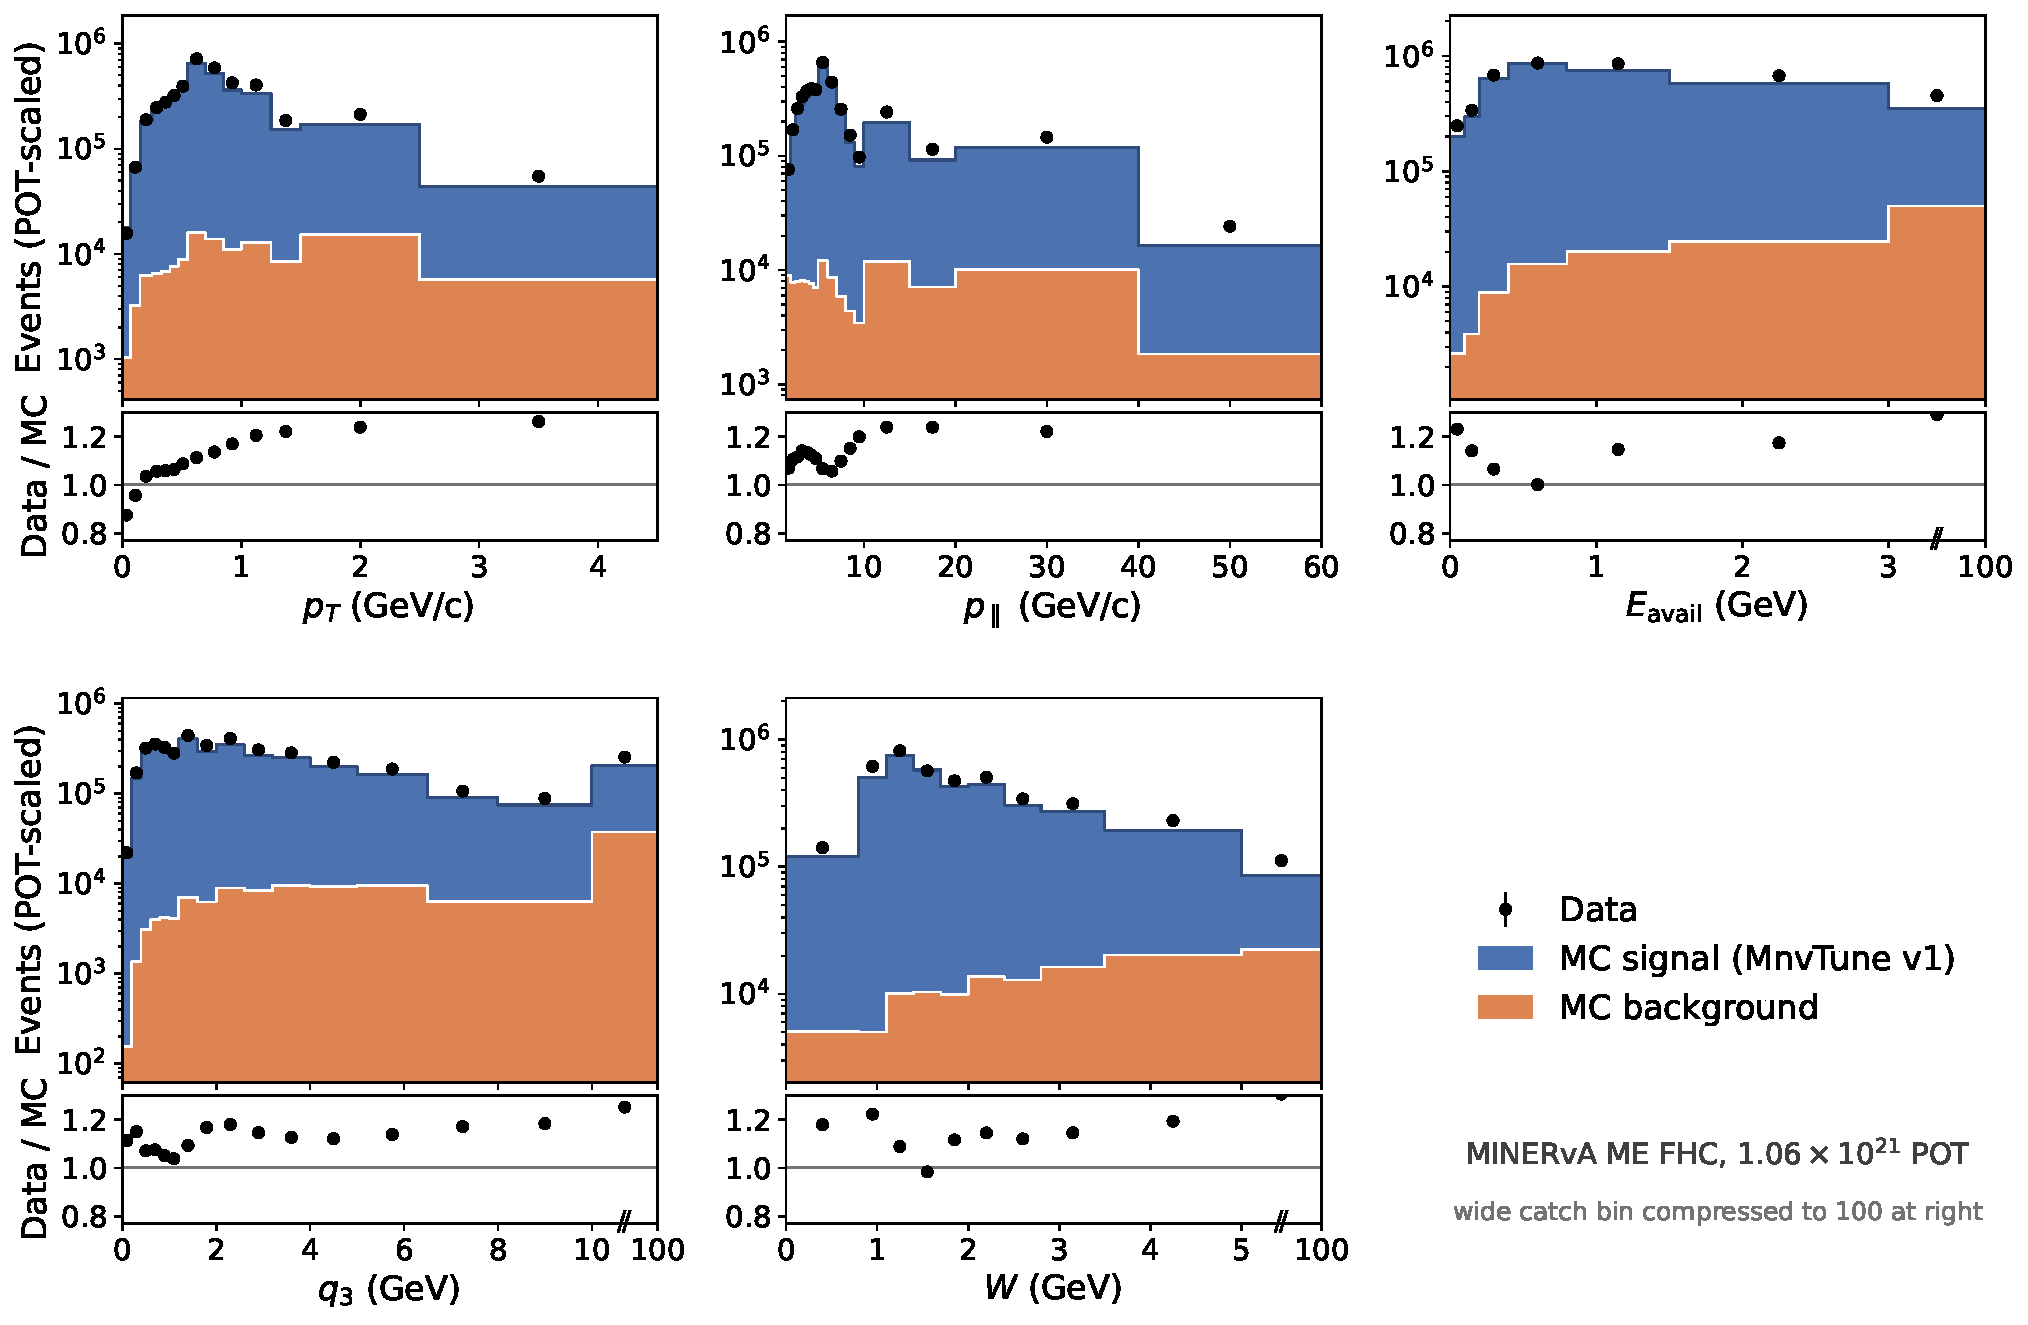
\includegraphics[width=0.99\textwidth]{control_plots}
  \caption{Reconstructed $\pT$, $\pPar$, $\Eavail$, $q_{3}$ and $W$ for the
  analysis selection. Data points overlay POT-scaled simulated signal (blue)
  stacked on background (orange); data/MC ratios appear below. Wide hadronic
  catch bins extend to \SI{100}{GeV} and are compressed at each panel's right
  edge. The gray MC-statistical band on the ratio is mostly narrower than the points.
  The $\sim\SI{12}{\percent}$ data normalization excess over MnvTune v1
  reflects the truth-level generator deficits in \S\ref{sec:3d-models}.}
  \label{fig:control}
\end{figure}

\begin{figure}[H]
  \centering
  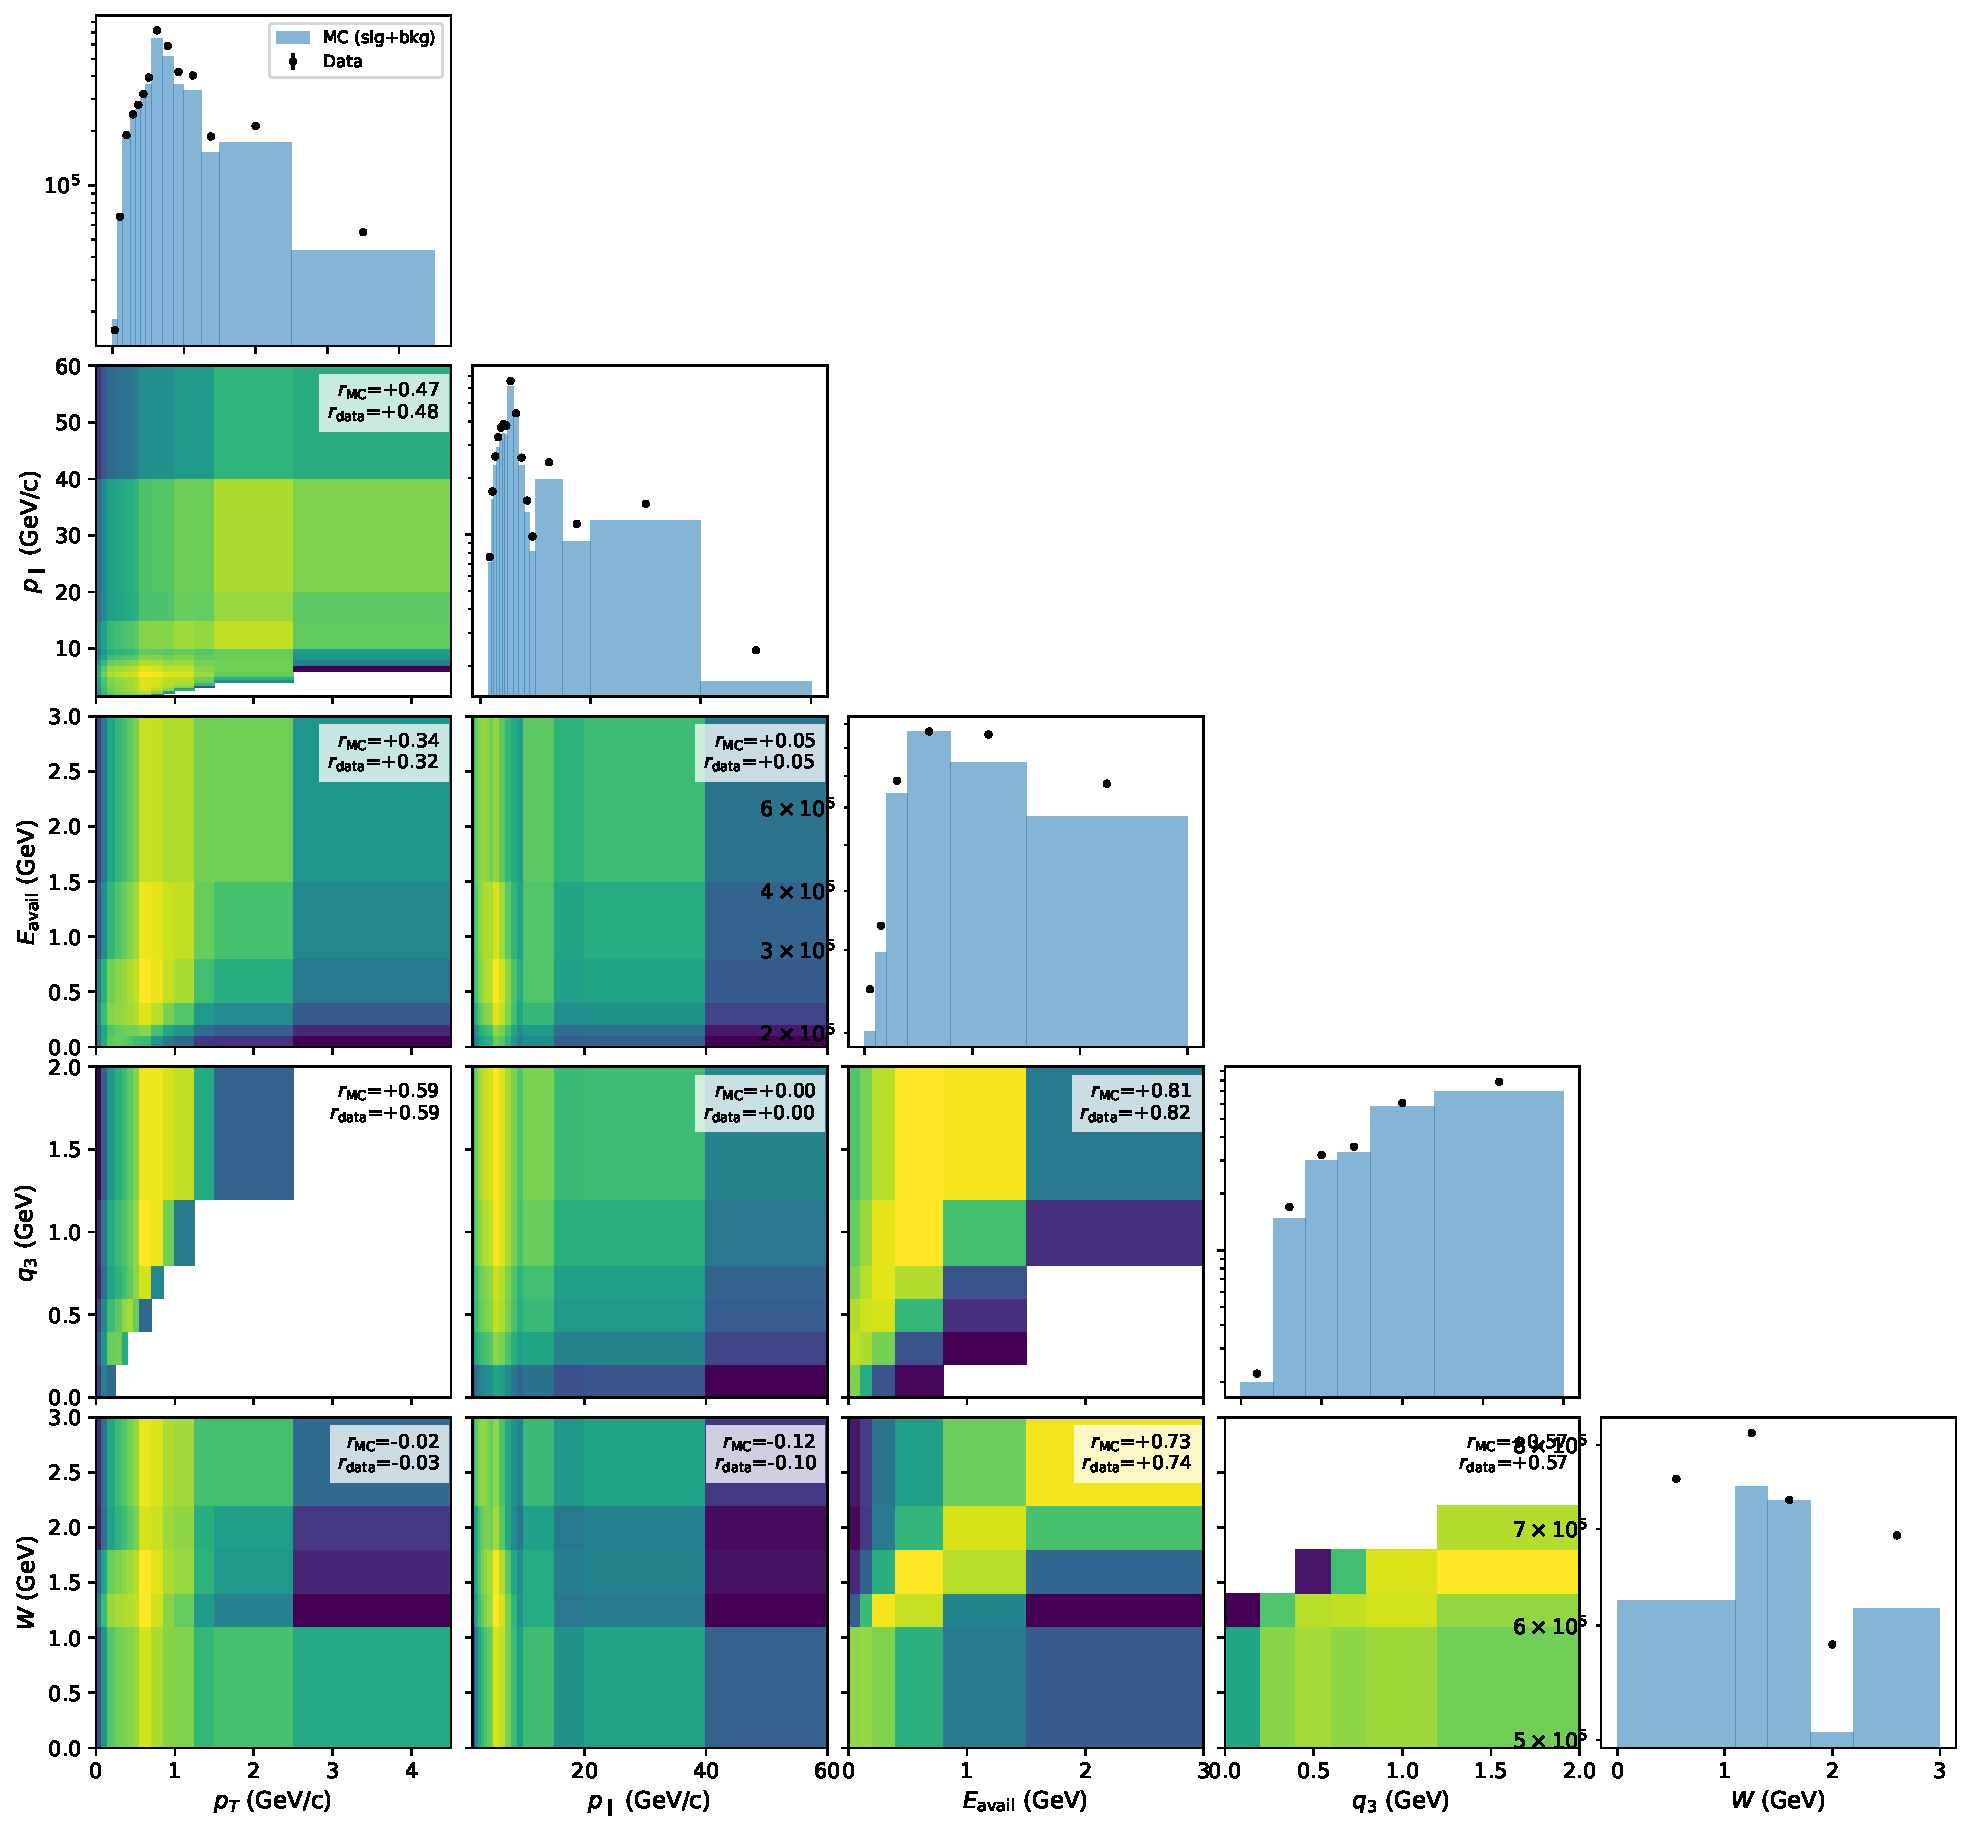
\includegraphics[width=0.92\textwidth]{control_corner}
  \caption{Reco-level corner plot of five observables. The lower triangle
  shows pairwise POT-scaled MC (signal$+$background) densities on a logarithmic
  color scale, with wide catch bins dropped. Each panel annotates the
  simulation's weighted Pearson correlation and the corresponding data value.
  The diagonal shows 1D marginals (data points over MC). The strongest
  correlations follow from kinematics: $q_{3}$ with $\Eavail$ ($r\approx0.81$)
  and $W$ with $\Eavail$ ($r\approx0.73$) share recoil energy; $q_{3}$ with
  $\pT$ ($r\approx0.59$) shares the muon transverse kick. Both $\Eavail$ and
  $W$ are nearly uncorrelated with the muon variables. Data reproduce every
  simulated coefficient within $0.02$.}
  \label{fig:control-corner}
\end{figure}

\section{The unbinned OmniFold procedure}
\label{sec:method}

\subsection{Algorithm}
\label{sec:method-algo}

OmniFold~\cite{Andreassen:2019cjw,Andreassen:2021zzk} unfolds by iterated
reweighting with machine-learned likelihood ratios, operating on per-event
observables rather than on a fixed histogram binning. Each iteration has two steps:
\begin{enumerate}[itemsep=2pt]
  \item \textbf{Step 1 (detector space).} A classifier separates measured
        data from reconstructed simulation weighted by the current
        push-weights. Its calibrated output $p$ gives the likelihood-ratio
        reweight $w = p/(1-p)$ for each reconstructed simulated event.
        Each simulated event is a (truth, reco) pair, allowing the weight to
        be \emph{pulled back} directly to its truth record. Truth events
        without a reconstructed partner (``misses'') receive step-1 weights
        from a regressor trained on the reconstructed subsample,
        $w(\mathrm{truth\ features})$. This native OmniFold acceptance
        treatment requires no separate efficiency correction.
  \item \textbf{Step 2 (truth space).} A second classifier separates the
        original truth-level simulation from the same sample carrying the
        pulled-back step-1 weights. Its smooth truth-space reweight becomes
        the next iteration's push-weight.
\end{enumerate}
After $n$ iterations, the push-weights define an efficiency-corrected
truth-level reweighted simulation ensemble. Histogramming this ensemble in any binning
chosen afterwards gives the unfolded spectrum. The iteration count and
learner capacity regularize the unfold.

\paragraph{Background subtraction (the one binned step).}
All selected data events enter step 1; none is discarded and no
negative-weight events are injected. Each receives a reco-bin \emph{purity}
weight. The POT-scaled background prediction includes genuine backgrounds
and out-of-phase-space signal (\S\ref{sec:selection}) and is binned on the
reconstructed analysis grid. A data event in reco bin $b$ receives
\begin{equation*}
  w_{\mathrm{pur}}(b) \;=\;
  \max\!\bigl(0,\; N_{\mathrm{data}}(b) - N_{\mathrm{bkg}}(b)\bigr)
  \big/ N_{\mathrm{data}}(b),
\end{equation*}
the predicted signal purity, floored at zero in the rare bins where the
background prediction exceeds the data. The step-1 classifier retains the
full unbinned kinematics. Binning enters only through this multiplicative
correction, an ${\sim}\SI{3}{\percent}$ effect overall, largest where
backgrounds concentrate (\S\ref{sec:selection}).

This correction is, deliberately, the one place the analysis binning enters
before the final histogramming. Other experiments' treatments are summarized in
\S\ref{sec:intro}. Our per-reco-bin weight is a conservative middle ground
at the sub-percent genuine-background scale. A fully unbinned alternative
injects negatively weighted background simulation on the measured side,
targeting the identical background-subtracted density $(D-B)/S$. It
reproduces the binned correction to \SI{\nwPctTot}{\percent} on the total
2D cross section and its systematic and statistical covariances to within
\SI{2}{\percent} (App.~\ref{app:negweight}). It removes residual binning
dependence and suits the extended-fiducial analysis, where backgrounds are
larger. It is not adopted, and the quoted extended-fiducial value does not
use it (App.~\ref{app:negweight}).
% Background-practice survey (H1/LHCb/ATLAS, OmniFold-HI, generative unfolding),
% production history and the Huang et al. comparison moved to sec_intro.tex
% ("Prior OmniFold applications"); the n=5 rationale moved to "Hyperparameter
% choice" below.

\subsection{Estimators and configuration}
\label{sec:method-config}

Gradient-boosted decision trees (GBDTs) replace the original OmniFold neural
networks for the scalar unfolds. With at most five high-level features per
event, tree ensembles typically match or outperform neural
networks~\cite{Grinsztajn:2022tabular} and train deterministically and far
faster on CPU. Ref.~\cite{Milton:2025tools} demonstrates their effectiveness
for unbinned unfolding with few high-level features, complementing deep
models for low-level event representations. We use GBDTs for scalar unfolds
and a point-cloud transformer for a recoil-cluster representation
cross-check (\S\ref{sec:pet}). The PET cross-check omits the muon
and is therefore not a full-event unfold. Calibration tests and
MLP/transformer cross-checks test the implementation in
\S\ref{sec:3d-classifier}.

The engine supports interchangeable backends (component terminology and
code paths in App.~\ref{app:codebase}). The published central value uses
\texttt{exact}, sklearn \texttt{GradientBoosting} with single-threaded
exact-split CART.
% Provenance: the production launcher passed no \texttt{-{}-estimator} flag; the driver revision it ran
% (d1bc8813) had no estimator option and always used the exact backend.
The uncertainty ensemble --- the systematic universe sweep
and the Poisson bootstrap --- is produced with \textbf{LightGBM} ($100$ trees,
$8$ leaves, learning rate $0.1$; identical settings for the step-1 classifier,
step-2 classifier, and miss regressor), which both of those launchers request
explicitly; so is the training-seed scan. \emph{The central value and its
covariance are therefore not estimator-matched}, and whether the LightGBM
covariance describes the uncertainty of the exact-split central value has not
been measured: no exact-split bootstrap, universe sweep or seed scan exists.
This is an unmeasured transfer, not a demonstration that the quoted
uncertainty is wrong. The LightGBM central value at the bootstrap's training
seed (seed~1) and the exact-split central value differ by a median of
\SI{0.97}{\percent} per bin (maximum \SI{12.5}{\percent}), a per-bin median of
$1.3$ times the per-bin standard deviation of the statistical bootstrap block,
and no covariance block carries this difference. The \texttt{lgbm} seed scan measures \texttt{lgbm} seed
noise, the smallest budget component (App.~\ref{app:statmethods}); it does
not measure the backend difference.
% Source: ASSESSMENT-20261008-2d-estimator-pairing.md sec. 2.1, 3 (P01-P09b); state/uncertainty-preparation-
% 20261008/a/pairings.tsv P02 and a/verification.md (seed 1 vs E_C: 0.97/2.67/12.50 %, 1.30/2.76/8.32 sigma_S);
% reviewer recompute e/recompute/rc_pairing.json.txt; KNOWN_ISSUES 88.
The third backend, \texttt{hist}
(sklearn \texttt{HistGradientBoosting}, matched 8-leaf configuration), is
retained for method-dependence studies (\S\ref{sec:results-tension}).

The central value is a single exact-split run whose seed was not pinned: its
production launcher passed no seed, and the driver revision it ran had no seed
option, so scikit-learn's \texttt{random\_state} was \texttt{None}. (This follows from
the launcher and driver revision; the run's own log was not found, and the
product records no seed.) The run-to-run
variation of this estimator has not been measured. The seeds are pinned only in
the LightGBM ensembles: seed~1 for the Poisson bootstrap, seed~42 for the
universe sweep and its matched central value, and seeds 1--10 for the ML band
(\S\ref{sec:uq-ml}).
% Source: ASSESSMENT-20261008-2d-estimator-pairing.md sec. 2.1 and P01 (revision d1bc8813, launcher
% sbatch_unfold_2d_MEHFC.sh, job 53116554; executed-bytes log not found); P09b (E_C seed noise unmeasured).
% Later driver revisions add --seed and --estimator options; their defaults do not describe this run.

\paragraph{The four estimator configurations.}
The note and the article use four configurations, all with five OmniFold
iterations, and each result names the one it uses:
\begin{enumerate}[itemsep=1pt, topsep=2pt]
  \item the 2D central value: the \texttt{exact} backend above, with purity-based
        background subtraction (\S\ref{sec:method-algo});
  \item the 2D uncertainty ensembles: the LightGBM backend above;
  \item the three- to five-dimensional central values: LightGBM at the same matched
        capacity (100 trees, 8 leaves), with purity-based background subtraction
        (\S\S\ref{sec:3d}--\ref{sec:eavailw});
  \item the joint-test estimator: a deterministic LightGBM variant with the unbinned
        negative-weight background treatment (App.~\ref{app:negweight}), whose
        refinement classifier has 400 trees and 31 leaves. The negative-weight
        treatment reduces the purity method's nominal-truth bias in the highest-$W$
        column at least fifteen-fold (from \SIrange{3.5}{4.1}{\percent} to
        \SIrange{0.11}{0.24}{\percent}, the level of the no-background closure), and the larger refinement classifier
        removes most of the background-related bias that remains
        (\S\S\ref{sec:val-negweight}--\ref{sec:val-departure}). It was selected
        before the joint-test design was frozen (\S\ref{sec:joint5d}).
\end{enumerate}
% Configuration 3: sec_5d.tex (100 trees, 8 leaves; purity footing) for 5D; the 3D/4D drivers default to
% --estimator lgbm and the purity bkg-mode (review 2026-10-11). Added 2026-10-11 so that this subsection is the single home the article cites for all four configurations;
% before, configurations 3-4 were described only in the article and in sec_5d.tex.

\paragraph{Hyperparameter choice.}
The learner settings were fixed \emph{a priori} rather than tuned on data. They are the sklearn
\texttt{GradientBoosting} defaults: 100 trees, learning rate $0.1$, and
depth-3 capacity. The uncertainty-ensemble LightGBM backend uses matched capacity
($\texttt{num\_leaves}=8=2^{3}$), giving every backend the same deliberately
modest capacity, one of OmniFold's regularizers (\S\ref{sec:method-algo}).
No hyperparameter search was performed on data, avoiding a tuning-on-result
loop. The configuration is instead validated after the fact by closure and
classifier-calibration tests (\S\ref{sec:validation},
\S\ref{sec:3d-classifier}), insensitivity to doubling the iteration count
(below), backend agreement in method-dependence studies
(\S\ref{sec:results-tension}), and an explicit training-seed variation band
for residual ML stochasticity (\S\ref{sec:systematics}).

Production uses $n=5$ iterations. Huang \emph{et
al.}~\cite{Huang:2024omnifold} select 45 iterations for OmniFold-family
methods (20 for their binned benchmark) using a binned $\chi^{2}$ against
known mock-data truth, a criterion they note is infeasible on real data.
We do not adopt that recommendation. Their mock data injects a large
prior--data \emph{shape} discrepancy through an RPA-modified quasielastic
model, requiring many iterations. Our prior already describes the data
shapes well (\S\ref{sec:controlplots}); the data pull is dominantly a
normalization. Cross-experiment production also typically uses
${\sim}5$ iterations~\cite{unbinnedguide}. Our $n=5$ is instead justified
empirically: doubling it to $n=10$ moves the total cross section by
\SI{0.026}{\percent} (\S\ref{sec:validation}), and the unfold reproduces
an independently published binned measurement of the same data
(\S\ref{sec:results}).

\subsection{MINERvA driver and pipeline conventions}
\label{sec:method-driver}



The higher-dimensional MINERvA driver (App.~\ref{app:codebase}) extends the
2D driver using an axis list and the same 2D helpers. The first two axes
are always $(\pT,\pPar)$, carrying the fiducial gate and per-$\pT$ flux.
Higher-dimensional runs extend the muon observables $(\pT,\pPar)$ with
$\Eavail$, $q_{3}$, $W$ in the phase space of \S\ref{sec:selection}.
Every production, universe-sweep, and closure run follows these conventions:
\begin{itemize}[itemsep=2pt]
  \item \textbf{Reco-space masking.} The measured events entering step-1
        training are exactly those passing the reconstructed-level
        selection; nothing outside the reconstructed phase space reaches the
        classifier.
  \item \textbf{Fake-free step-1 training.} Step 1 targets the purity-weighted background-subtracted data of
        \S\ref{sec:method-algo}. Genuine backgrounds \emph{and}
        out-of-phase-space signal fakes are removed from the data side.
        The simulated reco sample is fake-free by construction, so neither side of the step-1
        training contains events whose truth lies outside the
        measurement phase space.
  \item At histogramming, each simulated truth event carries its final
        OmniFold push-weight times its central-value simulation weight,
        including MnvTune reweighting. No additional efficiency-histogram
        division is applied. Step-1 miss regression already gives an
        efficiency-corrected truth spectrum; dividing again would
        double-correct.
        % Development history: a failure mode that occurred once in
        % development and was caught by the marginal self-validation gate
        % (\S\ref{sec:validation}).
  \item \textbf{Closure mirrors production.} In closure tests the
        pseudo-data are simulated events passing both the reconstructed and
        truth selections, weighted identically to the production data path,
        so closure exercises the same code path as the measurement rather
        than an idealized shortcut.
\end{itemize}

% "What the pipeline refuses to do" (test-suite discipline) moved to
% app_codebase.tex.

\subsection{Cross-section extraction}
\label{sec:method-xsec}
The differential cross section follows from unfolded truth-level counts:
\begin{equation*}
  \frac{d^{n}\sigma}{d x_{1}\cdots d x_{n}}
  = \frac{U}{c\,\Phi\,N\,\mathrm{POT}\,\Delta x_{1}\cdots\Delta x_{n}}
    \times 10^{4},
\end{equation*}
where $U$ is the unfolded yield and $c$ the per-bin \emph{completeness}, the
fraction of truth events visible to the unfolding input. The event loop
explicitly appends truth-only misses, so every truth event enters and
$c\equiv1$ bin-by-bin. The factor remains a monitored self-check; dropping
misses would give $c<1$. $\Phi$ is the per-$\pT$ flux integral, broadcast
over other axes, $N$ the fiducial nucleon count
($3.2353\times10^{30}$), and POT the data exposure ($1.057\times10^{21}$).
The factor $10^{4}$ converts flux tabulated per square meter to the reported
$\si{cm^2}$ ($\SI{1}{m^2}=10^{4}\,\si{cm^2}$), giving units of
$\si{cm^2}$ per axis unit per nucleon. The implementation
(App.~\ref{app:codebase}) is self-tested to reproduce frozen
lower-dimensional extractions to $<10^{-12}$. Since
$\sigma\propto1/\Phi$, $\Phi$ varies per flux universe when building the
systematic covariance. This variation dominates the Flux band
(\S\ref{sec:systematics}).

\subsection{Binning}
\label{sec:method-binning}
% The reported binning follows \texttt{minerva\_paper\_anc/bin\_mapping.txt} (cited below).
The 2D grid has 14 $\pT$ $\times$ 16 $\pPar$ bins; 205 of 224 are
reported. The 19 unreported diagonal cells have
$\pT^{\mathrm{hi}}/\pPar^{\mathrm{lo}}>\tan20^{\circ}$. The extension axes use
$\Eavail$: $[0,0.1,0.2,0.4,0.8,1.5,3.0,100]\,\si{GeV}$;
$q_{3}$: $[0,0.2,0.4,0.6,0.8,1.2,2.0,100]\,\si{GeV}$;
$W$: $[0,1.1,1.4,1.8,2.2,3.0,100]\,\si{GeV}$.
Each ends in a wide catch bin to capture the full CC-inclusive tails in
marginals; truncating the top edge would break the marginalization anchors
of \S\ref{sec:3d-anchor}. Binning after unfolding allows these choices to
be revisited without re-running the unfold. App.~\ref{app:release}
(\S\ref{app:release-identities}) gives all five axes' edges.
\S\ref{sec:205bins} defines the 205 reported cells, with the authoritative
mapping in \texttt{minerva\_paper\_anc/bin\_mapping.txt}.

Neither underflow nor overflow appears in the reported product, by
construction rather than by truncation. Truth-level muon edges coincide with the
measurement phase space (\S\ref{sec:selection}); no signal is defined
beyond them. Hadronic axes span $[0,100]\,\si{GeV}$, with catch-bin edges
far beyond the kinematic reach at
$\langle E_\nu\rangle\sim\SI{6}{GeV}$, so the truth grids are exhaustive. A selected reco event outside the
grid is treated as unaccepted and excluded from the measured sample by
\S\ref{sec:method-driver}'s masking convention. Its in-phase-space truth
content is recovered by the miss treatment, as for any unreconstructed
event. The unbinned unfold has no response-matrix under/overflow to track;
reporting bins are applied once to events that all lie inside the grids.

Truth$\to$reco migration on the analysis binning (Fig.~\ref{fig:migration})
summarizes the smearing OmniFold must undo, although it uses no response
matrix. Median diagonal purity is $\sim0.6$ on every axis. These substantial
migrations require unfolding; a bin-by-bin correction would be badly biased.

The structure differs qualitatively between the muon and hadron sides.
The spectrometer muon measurement makes the $\pT$ and $\pPar$ maps nearly tridiagonal, with
migrations rarely exceeding one bin. Purity dips to
${\sim}0.45$--$0.5$ for $\pT$ and ${\sim}0.35$ for $\pPar$ where bins
are finest, recovering in wide edge bins. The calorimetric axes have
coarser bins but relatively broader, visibly asymmetric migrations.
$\Eavail$ preferentially migrates \emph{downward} because energy carried
by neutrons and other unresponsive particles is not collected. Diagonal
purity falls from $0.61$ in the lowest bins to $0.43$ in the highest.
$q_{3}$, built from $\Eavail$ and the muon, inherits a milder version of the same pattern.
$W$ compounds $\Eavail$ and muon smearing and has the broadest migrations;
two-bin shifts are common in the resonance region. The lowest-$W$
(quasi-elastic) bin remains purest at $0.71$.

\begin{figure}[H]
  \centering
  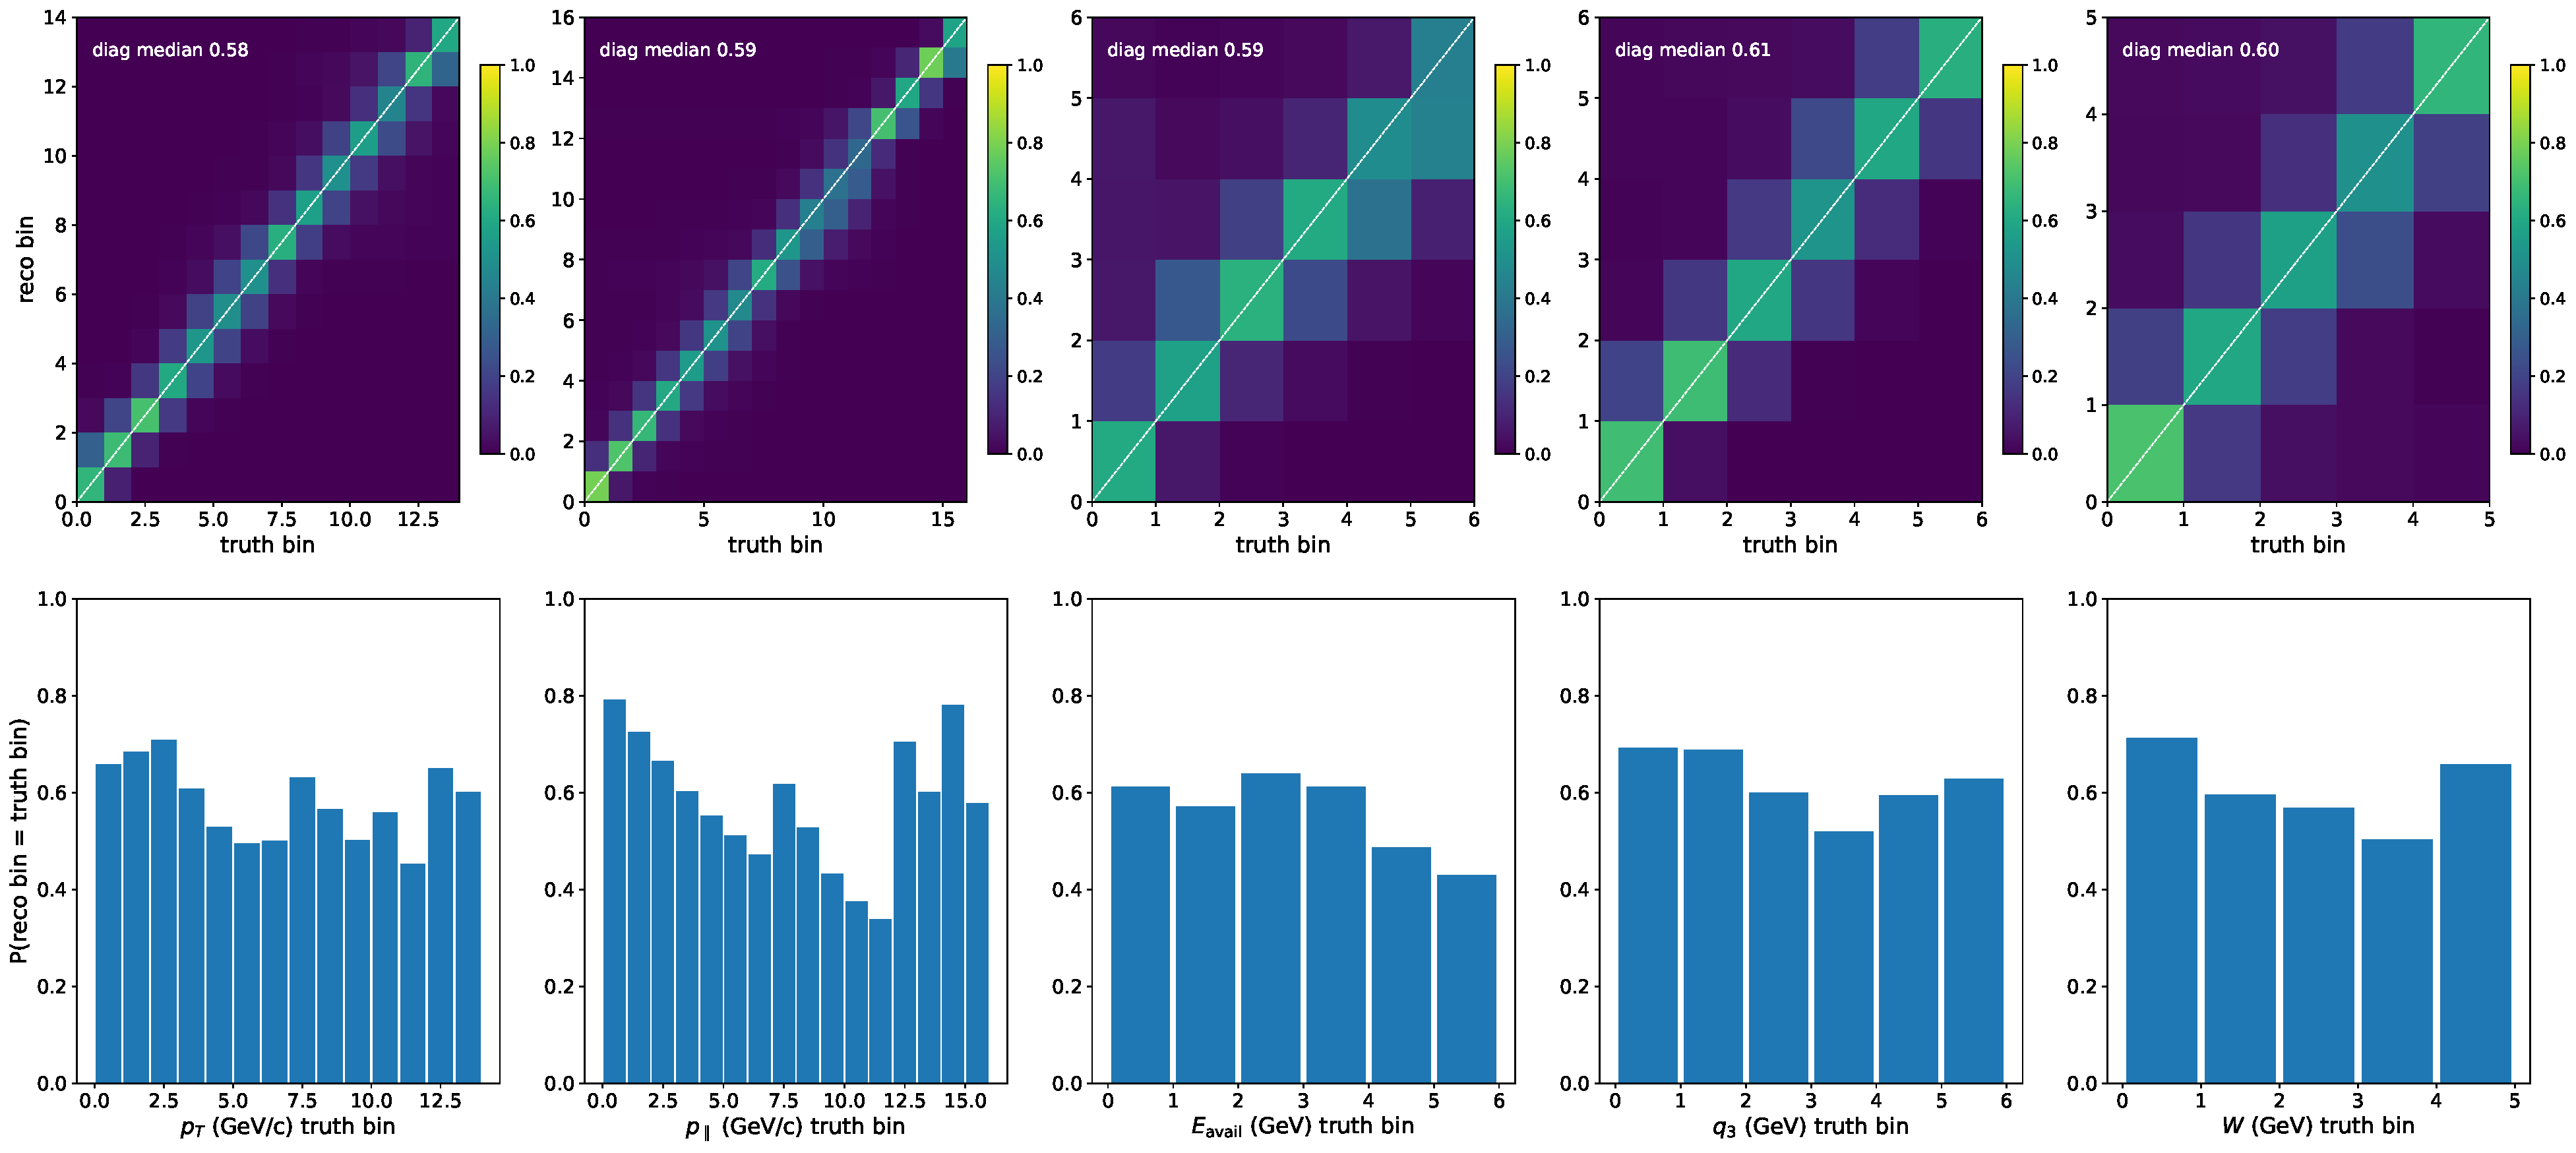
\includegraphics[width=0.99\textwidth]{migration_resolution}
  \caption{Simulated signal truth$\to$reco migration on the analysis binning
  for five observables. Top: column-normalized maps; bottom: diagonal purity
  per truth bin. Median diagonal purity is $0.58$--$0.61$ per axis.
  The figure is illustrative only; the unfold is unbinned.}
  \label{fig:migration}
\end{figure}

\subsection{Related developments and estimator scope}
Profile OmniFold~\cite{Zhu:2025profile} extends classifier-based EM to
forward-model nuisance parameters. Its distinct algorithmic construction
complements earlier unbinned profiled unfolding~\cite{Chan:2023tbf}.
Profiling nuisances with observed data would change our inference model,
which propagates an external nuisance ensemble through a fixed procedure.
Neither a profiled estimator nor its uncertainty is adopted here.

SPINUP learns a forward mapping~\cite{Butter:2025spinup}; AUSSIE replaces
OmniFold's second step with a different loss and avoids the outer
iteration~\cite{Ore:2026aussie}. Both offer possible future cross-checks
with different algorithmic assumptions. Reduced simulation-prior dependence
does not establish detector-model independence, adequate phase-space
support, or coverage for this measurement. Comparisons would require
matched signal, selection, normalization, and uncertainty definitions.

\section{Uncertainty quantification: constructing the covariance blocks}
\label{sec:systematics}

The uncertainty budget sums three blocks from systematic universes, statistical
bootstraps, and ML training-seed variation. Independence is an assumption;
distinct RNGs and physics sources alone do not establish it after unfolding.
All three 2D blocks are computed with the
LightGBM estimator, not with the exact-split estimator of the quoted 2D central
value (\S\ref{sec:method-config}). Whether the resulting covariance describes
that central value has not been measured. The historical 3D budget uses the analogous 3D grid construction
(\S\ref{sec:3d-syst}); no 4D uncertainty magnitude is reported (\S\ref{sec:4d}).
App.~\ref{app:statmethods} gives the full mathematics and worked examples using
the reported numbers. The resulting budget and its agreement with the published
total appear in \S\ref{sec:results-uq}.

\subsection{Systematic universes}
\label{sec:uq-universes}
Detector and model systematics use MAT-MINERvA's 44 error bands and 187
universes, identical to the published analysis's \texttt{GetStandardSystematics}
set. Each universe is re-unfolded with LightGBM at a fixed seed (seed~42),
against a reference central-value unfold with the same estimator and seed;
this reference is not the quoted exact-split one. Matching the learner and
seed does not ensure matching inputs: the adopted sweep's truth input
differs from this reference, as detailed below.
Per-band covariances follow MAT's universe-mean centering and biased $1/N$.
For a $\pm1\sigma$ pair, the covariance is the half-difference outer product,
excluding any common endpoint displacement from CV. The 100 PPFX universes
use the same mean-centered $1/N$ formula.

Top 2D bands: Flux \SI{\fluxBand}{\percent}, Muon\_Energy\_MINOS
\SI{2.31}{\percent}, MinosEfficiency \SI{1.47}{\percent},
Muon\_Energy\_MINERvA \SI{1.29}{\percent}. Figure~\ref{fig:uqbands} shows the
grouped fractional-uncertainty projections in the published Fig.~6/7 style
(the full $205\times205$ covariance projected exactly, $C_{1D}=PC_{2D}P^{\top}$,
before dividing by the 1D central value).

\begin{figure}[H]
  \centering
  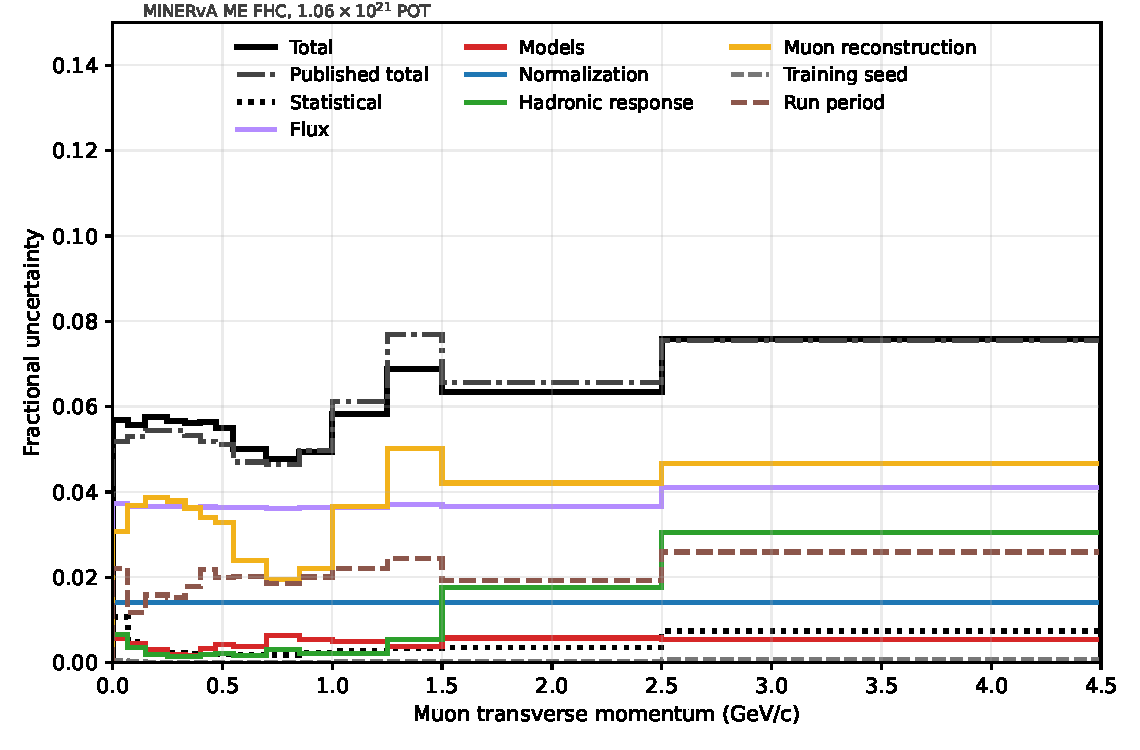
\includegraphics[width=0.49\textwidth]{MEFHC_fig6_7_uncertainty_pt}
  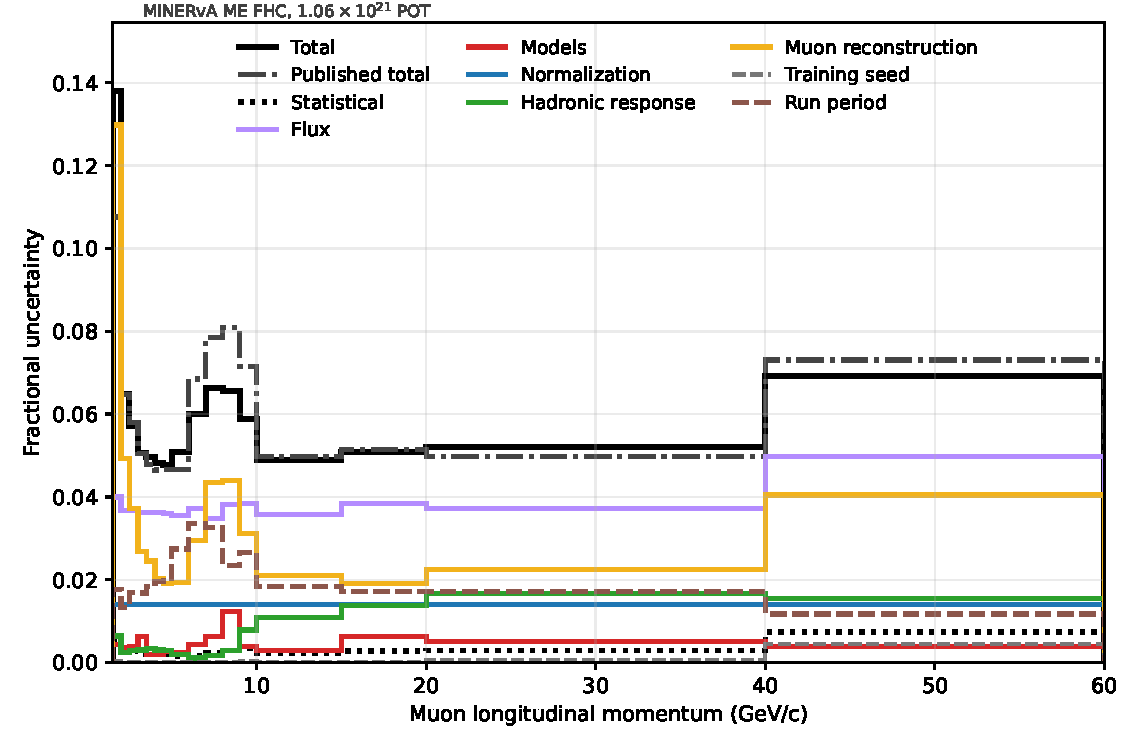
\includegraphics[width=0.49\textwidth]{MEFHC_fig6_7_uncertainty_pz}
  \caption{2D cross-section fractional uncertainty projected onto $\pT$
  (left) and $\pPar$ (right), grouped as in Figs.~6--7 of
  Ref.~\cite{MINERvA:2021owq} by flux, interaction models, normalization,
  hadronic response, muon reconstruction, and the statistical band.}
  \label{fig:uqbands}
\end{figure}

\paragraph{Flux $1/\Phi$ normalization.}
Varying $\Phi$ per flux universe in the dominant $\sigma\propto1/\Phi$ term
gives a Flux band of \SI{\fluxBand}{\percent}, versus
$\sim\SI{1}{\percent}$ when all universes use CV $\Phi$, and a standalone
combined budget of \SI{\uqMedian}{\percent}. Target-nucleon normalization
contributes a fully-correlated rank-1 band of \SI{1.4}{\percent}. The
100-universe flux covariance has participation-ratio effective rank
$\approx1$; one coherent normalization mode carries \SI{99.6}{\percent} of
the variance. Its leading mode correlates at $\rho=\rhoFluxMuon$ with the
rank-1 muon-energy-scale band in the rederived
Bashyal~\cite{Bashyal:2021tqu} joint block. The cross term is rank-2; two
independent estimators give $\rho=0.87$--$0.90$. Adding this block leaves
the systematic rank unchanged because its directions already lie in the
universe-covariance span (App.~\ref{sec:rank}).

\subsection{Statistical uncertainty: Poisson bootstrap}
\label{sec:uq-boot}
The statistical block jointly bootstraps data and simulation with 300 per-event
Poisson(1) weight replicas, each fully re-unfolded, using their sample covariance
(Fig.~\ref{fig:bootstrap}). Independent data and MC variance sources use two
independent sub-RNGs. MC reco and truth weights share a \emph{single} event
draw to preserve within-event migration correlations. Pinning the GBDT seed per replica
separates bootstrap and training-seed variances. The bootstrap block is
genuinely smaller than the published statistical block ($\approx2.55\times$ in
square-root trace). This \emph{observed} covariance difference does not
demonstrate a causal efficiency advantage. The data-only stream of the split
data/MC bootstrap ($C_{\mathrm{data}}/\texttt{StatOnly}=0.356$) shows the
difference is not a missing MC term, but cannot distinguish efficiency gain
from regularization bias or undercoverage (App.~\ref{sec:rank}). The fixed-truth coverage test
(\S\ref{sec:coverage}) found that the earlier statistical band undercovered
in its tails, unevenly across bins. The rebuilt band has not been independently
re-tested. The original test cannot decide between these explanations,
because its truth equals the prior.

\begin{figure}[H]
  \centering
  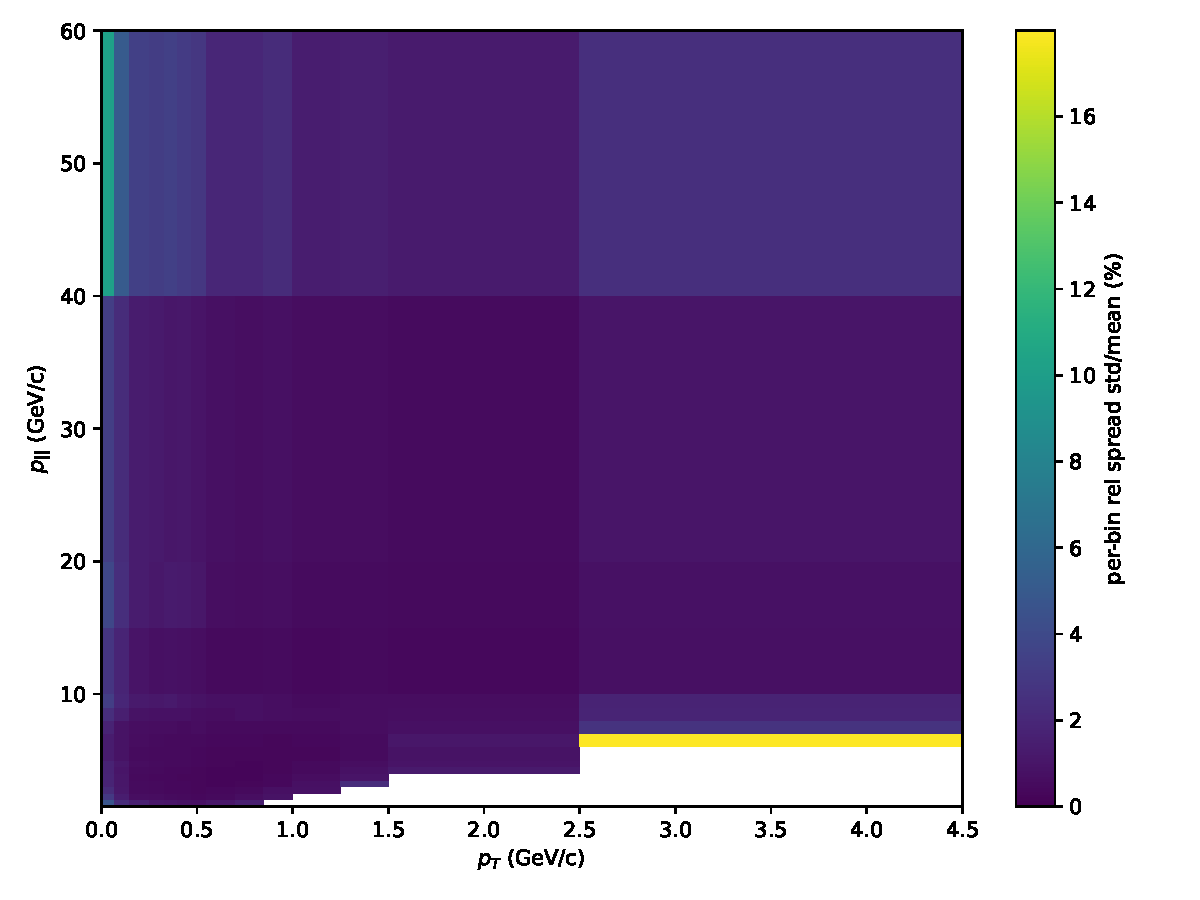
\includegraphics[width=0.49\textwidth]{uq_spread_2d}
  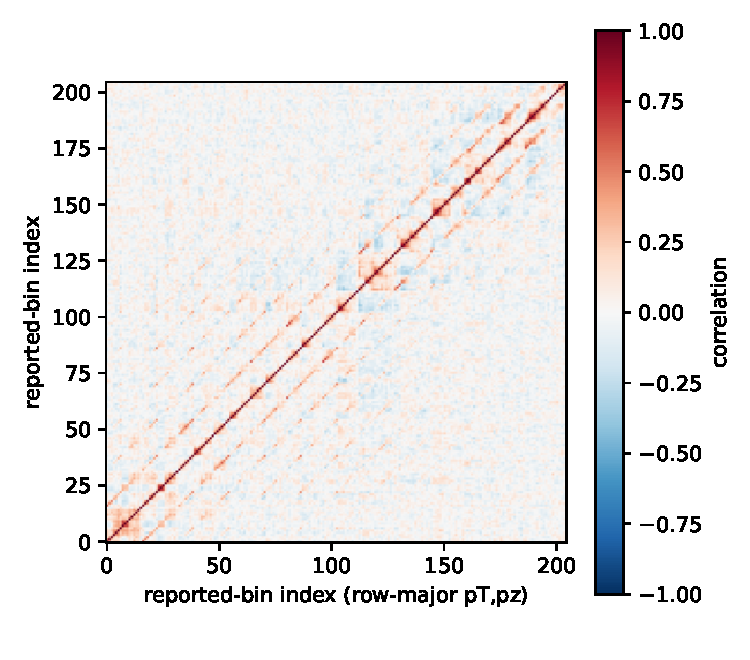
\includegraphics[width=0.49\textwidth]{uq_corr_2d}
  \caption{300-replica Poisson bootstrap per-bin relative spread of the
  unfolded 2D cross section (left) and correlation matrix for the
  205 reported bins (right).}
  \label{fig:bootstrap}
\end{figure}

\subsection{ML/optimization uncertainty: training-seed variation}
\label{sec:uq-ml}
The ML block is the sample covariance of re-unfolds with 10 independent
estimator seeds at fixed data and universe (Fig.~\ref{fig:seedscan}). It is
the smallest block, with median \SI{0.166}{\percent} per bin. Two refinements harden it: a
\emph{train/test-split} variant also re-draws the internal training split
and gives a band $1.24\times$ the pure-seed band used in the 2D budget of
Table~\ref{tab:uq}. The block measures LightGBM seed noise only: the
ten-seed LightGBM mean differs from the exact-split quoted central value by a
median of \SI{0.99}{\percent} per bin, a median of about five times this
block's per-bin standard deviation, so the block does not cover the backend
difference (\S\ref{sec:method-config}). The seed noise of the exact-split
estimator itself has not been measured.
% Source: ASSESSMENT-20261008-2d-estimator-pairing.md P09a/P09b; state/uncertainty-preparation-20261008/
% a/verification.md (lgbm 10-seed mean vs E_C: 0.99 % rel., 5.15 sigma_ML); reviewer recompute
% e/recompute/rc_pairing.json.txt "seedmean vs exact" 0.987 % / 5.147. The 0.28 % figure that stood here was not
% traced to an operand by the 2026-10-09 correction, and it did not name which central value it compared.
\begin{figure}[H]
  \centering
  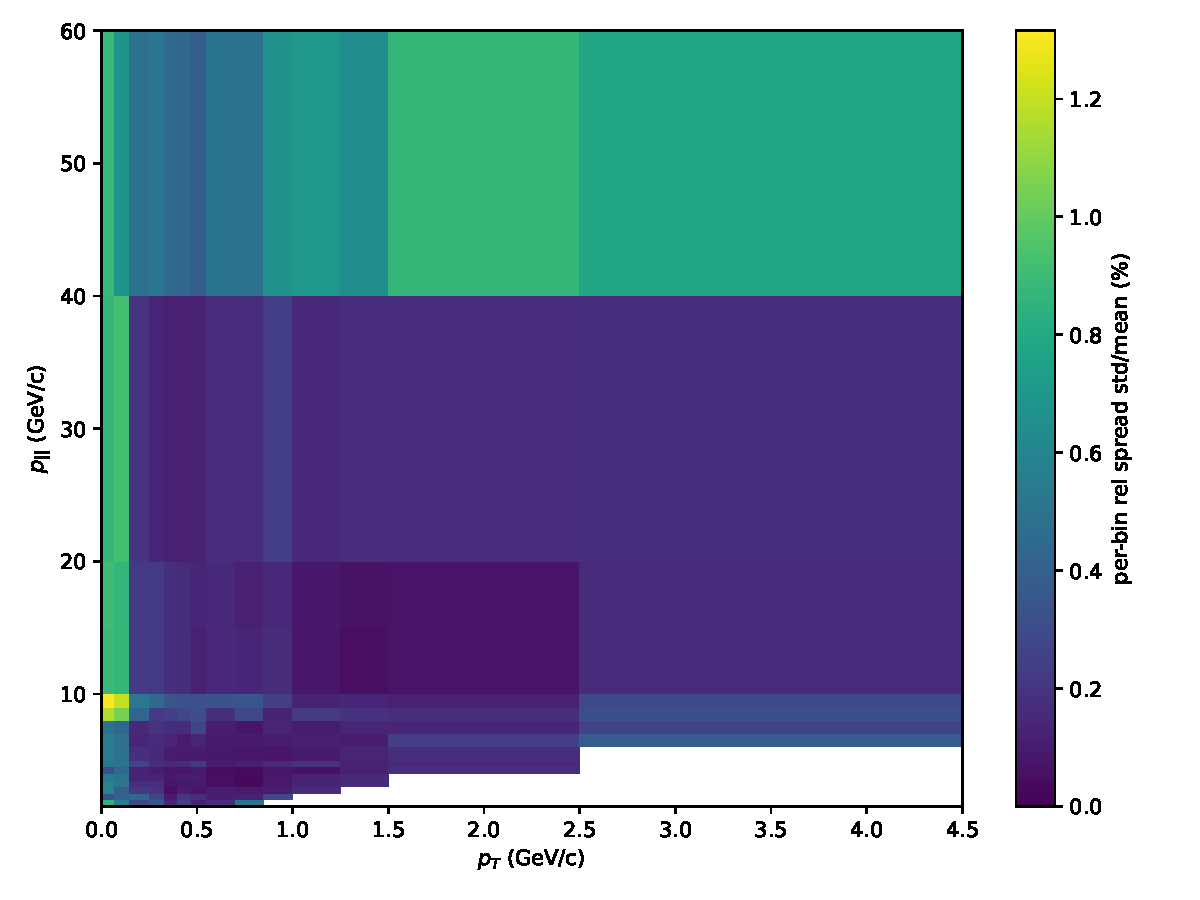
\includegraphics[width=0.49\textwidth]{seedscan_spread_2d}
  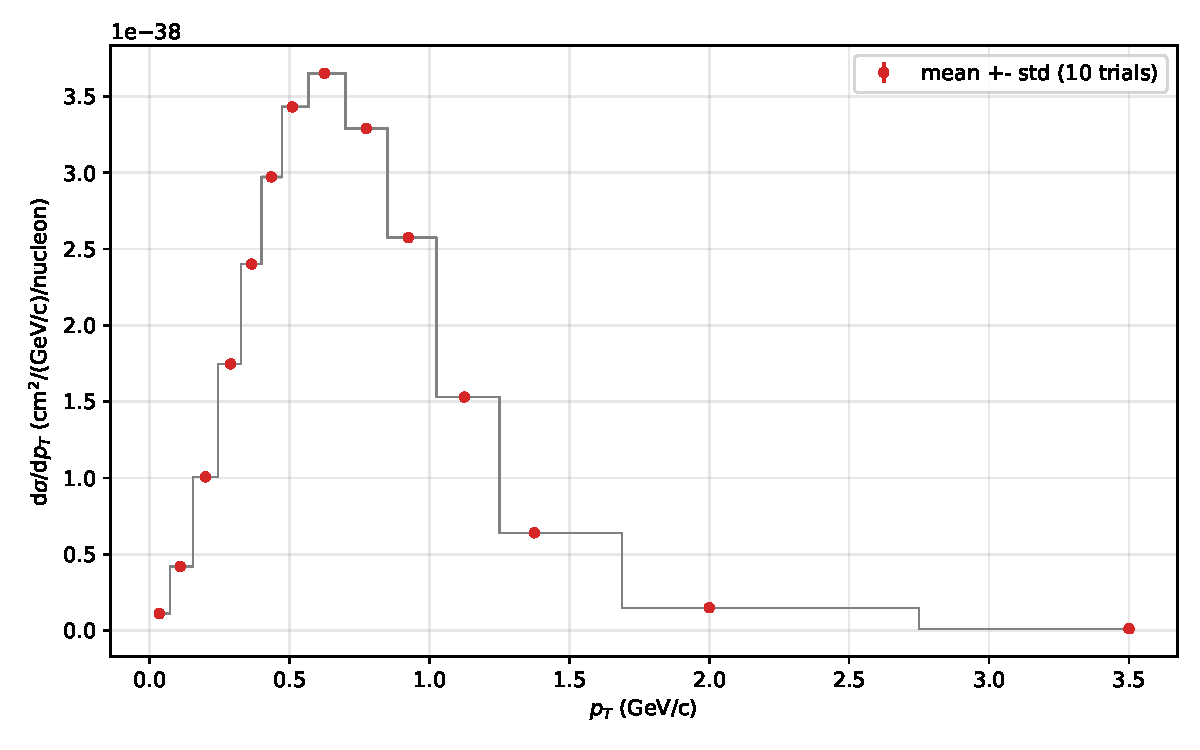
\includegraphics[width=0.49\textwidth]{seedscan_band_pt}
  \caption{ML training-seed variation over 10 estimator seeds, as per-bin
  relative spread (left) and fractional band projected onto $\pT$ (right).}
  \label{fig:seedscan}
\end{figure}

\subsection{Remaining checks of the 2D construction}
\label{sec:uq-2d-construction}
A saved-product and code review identifies additional construction issues
in the quoted 2D budget~\cite{TwoDFollowup2026}. The adopted May systematic
sweep uses a different simulated truth input from its seed-42 reference:
even a no-op EtaNCEL universe differs in all 205 truth-input cells, while
its saved reconstructed inputs agree. A common displacement cancels to
first order in the MAT mean-centered covariance; this observation neither
invalidates the entire covariance nor supplies a correction to subtract.
The July sweep does not have this mismatch. The unavailable May input and
code revision prevent a more specific attribution.

The Rvn1pi and Rvp1pi bands also encode the same shift under the configured
nonresonant-pion tune, counting it twice. This is a small, \SI{0.088}{\percent}
band, but a real construction defect; no conclusion about the published
analysis's implementation follows. The two examined small-input responses,
EtaNCEL and NormNCRES, are consistent with trainer instability contributing
at the ML-noise scale. They do not establish a mechanism for every small
band or justify subtracting an overlap from the budget.

Background-template statistics still require propagation or an unfolded
bound. In the saved reconstructed histograms their error exceeds one tenth
of the data's Poisson error in 60 of 205 bins, so neglecting them everywhere
is unsupported. This is a reconstructed-space diagnostic, not a measured
unfolded uncertainty. Selection-complete 2D lateral variations and the
identity of the PPFX universe indices between event weights and flux
normalization also require verification. These findings leave the printed
budget unchanged while identifying work needed to qualify its construction.

\subsection{Combination and the unified-throw test}
\label{sec:uq-combine}
The nominal covariance is the block sum
$C = C_{\mathrm{syst}} + C_{\mathrm{stat}} + C_{\mathrm{ML}}$, which assumes
the blocks are independent \emph{and} the unfolding responds linearly to
simultaneous perturbations, allowing per-band covariances to add. The
\emph{unified throw} directly tests linearity (App.~\ref{sec:universes};
\S\ref{sec:eavailw-construction}) by jointly re-unfolding all reweightable
knob bands and the flux multisim, perturbed simultaneously per event.
The corrected construction interpolates asymmetrically between actual
$-1\sigma$ and $+1\sigma$ event-weight endpoints, fixes the estimator seed
for every throw, and centers the joint covariance on the throw mean.
That mean's displacement from CV is stored separately as a per-bin vector
and its norm; per-band endpoint displacements are not stored. The matched
block comparator re-unfolds both endpoints using MAT's universe-mean
centering and biased $1/N$ normalization. A single-throw superposition probe
is insufficient to test nonlinear response. No scalar run-to-run jitter floor is
subtracted. The 5D result uses the strict joint ensemble and matched-endpoint
comparator.
% Implementation: nd-unfolding/unified_throw_cov.py

More generally, this reframes the block sum as an approximation --- valid only
where the unfolding responds linearly --- rather than as a default
construction.  We retain the per-source decomposition for attribution and use it only after
joint throws and matched block endpoints pass the stated validation tests.

\subsection{What changes for the higher-dimensional products}
\label{sec:uq-higherdim}
Dump-all shifted branches are limited to CV event-loop support. For the five
kinematic bands (BeamAngleX/Y, MuonResolution, and
Muon\_Energy\_MINERvA/MINOS), selection-complete active-universe event loops
are the production migration gate. They supply the adopted five-axis
covariance's lateral block; higher-dimensional products using dump-all lateral
branches remain candidates. Replacing the support-limited lateral block by the
selection-complete one moves that block's square-root trace by
\SI{\latTraceMove}{\percent}. That is a change in a square-root trace and is
\emph{not} a bound on any individual bin: across the \latBins\ reported bins
the per-bin ratio of active to support standard deviation runs \latRatioMin\ to
\latRatioMax, and within the top \SI{1}{\percent} of bins by support variance
--- which carry \SI{\latTopVarShare}{\percent} of the total --- it runs
\latRatioTopMin\ to \latRatioTopMax. A small share of the aggregate variance
does not make a bin irrelevant to a quoted result.

\paragraph{Scope of the selection-complete replacement.} The replacement covers
the five detector bands using shifted reconstructed kinematics. MINOS
efficiency and the three GEANT
hadron-interaction bands (GEANT\_Neutron, GEANT\_Pion, GEANT\_Proton) retain
their weight-based treatment and are thereby excluded from the kinematic
replacement. This classification does not independently validate
hadronic-response model completeness for the $\Eavail$ and $W$ measurement.

The corrected 5D ML ensemble fixes the estimator seed at 42 and varies the
train/test split seed. It therefore measures split response and does not measure full
estimator stochasticity. A dedicated scan of twelve estimator seeds at fixed
data and split closes this scope. Its covariance has
$\sqrt{\mathrm{Tr}\,C}=\SI{\gbdtAiEstTrace}{cm^2/nucleon}$,
\SI{\gbdtAiEstFrac}{\percent} of the candidate split-varied band
(\SI{\gbdtMlSplitTrace}{cm^2/nucleon}). Genuine estimator stochasticity therefore
dominates the adopted band over effects of the particular train/test partition.
The scan remains an auxiliary robustness check; it is not an independent
matrix, since split and estimator responses are not assumed uncorrelated. Both
bands are minor components, about three percent of the combined budget in
$\sqrt{\mathrm{Tr}\,C}$.

An earlier 5D candidate used both mean-centered and CV-centered unified
throws (\S\ref{sec:uq-combine}); no magnitude from either is quoted, and
neither is adopted. The adopted product is a later, separate
\texttt{cv}-variant build
(\S\ref{sec:eavailw-construction}; App.~\ref{app:history-5dcandidates}).
% Routed record (formerly App. E \texttt{gbdtfive-macros}; row removed 2026-10-04 because the
% sentence above rests on App. H, whose struck-values table cites it directly):
% \repopath{docs/orchestration/PROCEDURE-gbdtFive-macro-update.md}.

Per-universe background subtraction in all 187 universe unfolds and the CV
changes the combined \emph{block-sum} sqrt-trace by only
\SI{0.28}{\percent} and the \emph{adopted} covariance by \SI{0.18}{\percent},
a numerically negligible bound on the background-CV choice (App.~\ref{app:history}).
% (\SI{0.18}{\percent} is after the flux (J28) correction; App. H keeps the
% superseded-product wording and the inflation-damping explanation.)
The 4D and extended-fiducial results still lack covariances from this
procedure; the 5D covariance is not transferred to them.

% The chi^2 caveat formerly here moved to sec_results.tex (\S\ref{sec:results-compare}).

\section{Validation of the two-dimensional measurement}
\label{sec:validation}

In a simulated experiment, \emph{truth} is the known target distribution,
the \emph{prior} is the starting simulated truth distribution, and the
\emph{response} describes reconstruction and selection conditional on truth.
A closure test compares the unfolded estimate with its known target under a
specified deformation. Bias is the mean estimate minus that target over
repeated experiments; a single closure residual also contains sampling
fluctuations. Coverage is the fraction of repeated intervals containing the
specified truth, and tests the estimator and interval procedure together.
Table~\ref{tab:validation-questions} separates these questions before the
results. Repeating a numerical calculation checks neither interval calibration
nor the adequacy of the physical model.

\begin{table}[H]
\centering\footnotesize
\begin{tabular}{@{}p{0.16\textwidth}p{0.27\textwidth}p{0.25\textwidth}p{0.23\textwidth}@{}}
\toprule
Check & Target and estimator & Sample relation / measured quantity & Rule and conclusion \\
\midrule
Injected closure & Reweighted simulated truth; 1A LightGBM, five iterations & Same simulated response; residual under named truth or hidden-variable deformation & Thresholds below; passes depend on deformation and amplitude \\
\addlinespace
Miss completeness & Full truth inventory; production event mapping & Same event keys; truth-only entries retained & Membership and completeness invariants; no recovery or coverage claim \\
\addlinespace
Iteration stability & Same data; five versus ten iterations & Shared sample; movement of total and shape & Small observed movement; not a known-truth accuracy test \\
\addlinespace
Fixed-truth coverage & Fixed unfluctuated MC truth; LightGBM statistical estimator & Poisson pseudo-data; MC resampling shares the band's mechanism; pooled toy--bin containment & Predeclared coverage windows; earlier band fails. Rebuilt band awaits independent test \\
\bottomrule
\end{tabular}
\caption{Validation questions, targets and limits. Shared simulation is not an
independent detector-response test. Coverage pooled over bins is not a
simultaneous probability that every bin is covered.}
\label{tab:validation-questions}
\end{table}

\paragraph{Closure.}
Three existing closure families used playlist 1A, LightGBM and five iterations
(thresholds in parentheses).
% (1A lgbm 5-iter)
\begin{itemize}
  \item \textbf{Truth-reweight} (same factor for truth and reco weights):
        gaussian-$\pT$ residual \SI{0.046}{\percent}, tilt-$\pPar$
        \SI{0.013}{\percent} (thr \SI{1.5}{\percent}). Injected truth recovered.
  \item \textbf{Hidden-variable} (bias on $\Delta\pT=\pT^{\mathrm{reco}}-\pT^{\mathrm{truth}}$,
        a resolution variable outside the feature set): leakage linear in amplitude,
        $A=0.05/0.10/0.30\to0.57/1.14/3.43\,\%$ (thr \SI{3.0}{\percent});
        the first two amplitudes pass; the deliberately large $A=0.30$ arm exceeds
        the threshold.
  \item \textbf{Alt-model} (train on CV, pseudo-data from an alternative universe):
        MaCCQE \SI{0.068}{\percent}, Flux \SI{0.376}{\percent} (thr \SI{2.0}{\percent}).
\end{itemize}

\paragraph{Injected-feature recovery.}
The 2D gaussian-bump truth-reweight closure passes the unbinned-unfolding guide's
recovery test~\cite{Canelli:2025guide}. In the feature bins, the residual from injected truth is
\SI{1.69}{\percent} for an injected \SI{17.2}{\percent} feature
(ratio $0.098$), or $\approx10\times$ smaller. Recovery of the data's deviation
from the prior must leave a residual far smaller than the feature;
unfolding cannot manufacture discriminating power (3D: \S\ref{sec:3d-closure}).

The naive reco-vs-truth $\chi^2$ data-vs-prior test gives truth$>$reco.
As expected at high resolution, detector smearing lowers the
reco baseline and a stat-only diagonal omits unfolding covariance. The proper
full-covariance goodness-of-fit uses the $\chi^2$-vs-paper of
\S\ref{sec:results-tension} and the generator comparisons.

These closure tests validate the estimator; they are not used to assign a non-closure
uncertainty. Such an uncertainty would require a predeclared suite
of injection shapes and amplitudes rather than calibration to a single
Gaussian bump.

They do not test pseudo-data with a detector response that disagrees
with the unfolding response. Appendix~\ref{app:response-mismatch} defines a
complementary record-only $\Eavail$ response-mismatch closure and a more complete
leading-nucleon follow-up. No result from that test is claimed here.
\S\ref{sec:val-fiveaxis} validates the five-axis estimator, including background
subtraction.

\paragraph{What the remaining validation needs.}
The follow-up assessment~\cite{TwoDFollowup2026} distinguishes a proposed
split-sample width check from repeated-sampling coverage. With a fixed MC
bank, binning maps and purity correction, such a check can support only
conditional precision at its tested exposure; nonlinear unfolding does not
guarantee a simple half-to-full-exposure scaling. It cannot supply the
variation across independent MC populations. The original objective of
validated total uncertainties for all 205 bins, the integral and the
projections has no feasible route with the current inputs. It requires
independent populations or a validated generative law, a continuous
nuisance generator for total-interval tests, an untouched generator-truth
domain for bias checks, and the construction repairs in
\S\ref{sec:uq-2d-construction}. This is a limitation of the available
evidence, not a general impossibility result for 2D unfolding.

\subsection{Fixed-truth coverage of the 2D statistical band}
\label{sec:coverage}
This test asks whether the production 2D statistical band (\S\ref{sec:bootstrap}) covers a
\emph{fixed} truth at its nominal rate. Its design, criteria and positive control were
pre-registered before any toy ran (App.~\ref{app:provenance}, \texttt{coverage-fixed-truth}).

Each toy draws pseudo-data event by event as Poisson counts with means equal to the simulated
reconstructed weights. It resamples the simulation with the production Poisson(1) bootstrap, and
unfolds with the statistical band's estimator (lgbm, five iterations, fixed training seed), the
learner of the quoted central value at a different seed (\S\ref{sec:method-config}). The reference
$T$ is the unfluctuated simulated truth, identical in every toy. The no-fluctuation configuration
reproduces both the production closure output and $T$ exactly.

In reported bin $b$ of toy $t$, $z_{tb}=(U_{tb}-T_b)/(r_b T_b)$, where $r_b$ is the production
band's relative spread. Coverage $C_k$ is the fraction of all (toy, bin) pairs with $|z|\le k$,
with intervals from resampling whole toys. The band counts as nominal if its ratio to the true
scatter lies in $[0.9,1.1]$, which gives the windows $C_1\in[\covTwoDWinOneLo,\covTwoDWinOneHi]$
and $C_2\in[\covTwoDWinTwoLo,\covTwoDWinTwoHi]$. A FAIL at the interim look of 100 toys, with
99.5\% intervals, stops the study.

\textbf{The band fails: it undercovers in its tails.} At the interim look
($N_{\text{toy}}=\covTwoDNtoy$, 205 bins):
\begin{itemize}[nosep]
  \item $C_1=\covTwoDCOne$ $[\covTwoDCOneLo,\covTwoDCOneHi]$ is nominal (Gaussian 0.683).
  \item $C_2=\covTwoDCTwo$ $[\covTwoDCTwoLo,\covTwoDCTwoHi]$ lies entirely below its window
        (Gaussian 0.954).
  \item The pull RMS is $\covTwoDPullRMS$, and the mean pull is consistent with zero.
\end{itemize}
The pre-registered verdict is FAIL-undercoverage, and the study stopped by its futility rule. An
independent recomputation with its own code reproduces the pooled coverages, their intervals, the
controls and the secondary below.

The positive control rescales the band on the same toys. At $\times0.7$ and $\times1.3$, $C_2$
moves to $\covTwoDCTwoLowCtl$ and $\covTwoDCTwoHighCtl$, and both directions are flagged.

The failure is one of width, not bias. The per-bin pattern below is descriptive and post hoc.
\begin{itemize}[nosep]
  \item \textbf{Uneven in both directions.} The band is too wide in $\covTwoDNwide$ bins (pull RMS
        below 0.9) and too narrow in $\covTwoDNnarrow$ (above 1.1). The pooled $C_1$ is nominal
        partly through this cancellation; the median bin's pull RMS is $\covTwoDBinRMSmed$.
  \item \textbf{Where it is too narrow.} $\covTwoDNlowCTwo$ bins have a per-bin $C_2$ below 0.85.
        Of these, 21 form a block at $\pPar\ge\SI{15}{GeV/c}$ and $\pT<\SI{0.55}{GeV/c}$. Six more
        lie in the highest-$\pT$ row (\SIrange{2.5}{4.5}{GeV/c}) at $\pPar$
        \SIrange{6}{20}{GeV/c}. The $\covTwoDNedge$ bins with pull RMS above~2 carry
        \SI{\covTwoDDeficitShare}{\percent} of the $C_2$ deficit.
\end{itemize}

The band's replicas divide by a bootstrapped completeness that the central value (exactly~1)
does not carry. A secondary, added by amendment after the pilot, applies that division to the toys.
Scored against the same band, it overcovers: $C_1=\covTwoDRepCOne$, with its interval above the
window. By the rule fixed before the full run (its undercoverage branch was written after the
pilot pulls had been seen), the primary undercoverage is attributed to this term of the band's
construction. The attribution is partial: in the replica form, the $\pPar$
\SIrange{40}{60}{GeV/c} column still undercovers.
That term was removed on 2026-10-06 and the band rebuilt; the rebuilt band is the quoted one
(\texttt{KNOWN\_ISSUES.md} 84; App.~\ref{app:provenance}, \texttt{coverage-fixed-truth}). This
section's result is for the earlier band and was not re-tested.

\textbf{The rebuilt band, scored post hoc.} Rescoring the same 100 toys against the rebuilt band,
which is post hoc and partly circular (its MC part reuses the toys' resampling mechanism), removes
the tail undercoverage: $C_2=0.977$ $[0.974,0.980]$ and $C_1=0.781$ $[0.771,0.790]$, both above
their nominal windows, so the rebuilt band is wider than the toy scatter (pull RMS 0.84, mean pull
consistent with zero). The residual excess width lies in the data-statistics component: the
per-bin pull RMS falls as that component's share of the band's variance rises, which corresponds
to a data-statistics part about $1.6\times$ wider in $\sigma$ than the toys produce. Background
purity does not explain it. Its cause is not established. A post hoc bootstrap-on-one-toy
diagnostic, with a decision rule committed before it ran, is consistent with the closure toys
under-scattering, because their pseudo-data sit on the training MC events, rather than with the
data bootstrap over-scattering; it is neither an independent-population coverage test nor a
real-data calibration. The held-out-MC re-test that would separate the two is deferred until
after the publication package (\texttt{KNOWN\_ISSUES.md} 85). Split-sample width checks that
condition on the existing MC bank, binning maps and purity cannot establish repeated-sampling
coverage across independent populations, so validated total intervals over the full reporting
domain need new inputs as well as the construction repairs of \S\ref{sec:uq-2d-construction}.
% Source: state/ki84-rebuild-20261006/rescore_vl169_toys_vl170.json (vl170: C1 0.7806 [0.7709, 0.7902],
% C2 0.9769 [0.9737, 0.9800], pull_rms 0.843, pull_mean -0.027 [-0.058, 0.004]; label "POST HOC, DESCRIPTIVE";
% commit 5aab2d6d); KNOWN_ISSUES.md 85 (the 1.6x, the f-share regression, purity median 0.975);
% DECISION-RULE-20261006-ki85-bootstrap-diagnostic.md (outcome (b)); diagnostic 8eb40e5f. Moved here from the
% article on 2026-10-11, when its 2D-coverage subsection was shortened.

\textbf{Scope.} The result concerns the statistical band only.
\begin{itemize}[nosep]
  \item It changes no central value or quoted uncertainty.
  \item It tests the LightGBM statistical estimator at the band's training seed (seed~1), not at
        the quoted central value's seed~42.
  \item It says nothing about systematic, total or five-dimensional coverage.
  \item Its simulation-side scatter reuses the resampling that built the band, so only the
        data-side fluctuation is tested by an independent mechanism.
  \item Because $T$ equals the prior, it cannot detect regularization bias toward the prior.
\end{itemize}

\subsection{Other validation diagnostics}
\label{sec:val-other}

\paragraph{Unbinned diagnostic (C2ST).}
The classifier two-sample test (C2ST) AUC drops from $\approx0.535$ before
unfolding to $\approx0.501$ after, indicating removal of the reconstructed
data\,$\leftrightarrow$\,MC mismatch. A classifier is trained to separate the data from the
(reweighted) simulation in the full unbinned feature space, and its held-out AUC/accuracy is
compared to the chance value $0.5$. This binning-free check is strictly
\emph{descriptive}; we do \emph{not} quote a calibrated $p$-value. The C2ST as run
trains and evaluates on the same sample without cross-fitting. A valid null
would require re-running the full cross-fitted OmniFold pipeline per
pseudoexperiment. Calibrated unbinned goodness-of-fit remains
open~\cite{Canelli:2025guide}.

\paragraph{Same-ensemble pull diagnostic (not a coverage test).}
An earlier ensemble contains $N_{\text{toy}}=200$ 2D closure unfolds
(App.~\ref{app:provenance}, \texttt{coverage-toys}),
% (\texttt{sbatch\_coverage\_toys\_MEFHC\_200.sh}; rollup
% \texttt{uq/coverage\_toys.py}, summary \texttt{uq/coverage/coverage\_summary.txt})
with weighted MC reco pseudo-data and truth marginals stored in truth
histograms. Each uses its own bootstrap seed $k$ and per-event Poisson(1) draws,
as in production; seeds avoid collisions with production replicas.
% CLI: \texttt{-{}-closure} with \texttt{-{}-bootstrap-seed $k$}; truth histogram \texttt{hTruthXSec2D}
Toy seeds are independent; bins within a toy are correlated. The MC bootstrap
multiplies the truth weight, fluctuating both the unfolded result and stored truth.
% truth weight: \texttt{w\_truth}; stored truth: \texttt{hTruthXSec2D}
Stored truth varies in all 205 reported bins, so its all-toy mean
$\bar X^{\text{truth}}$ is not an independent fixed truth for a split-sample
coverage claim; it only centers a same-ensemble diagnostic.

In reported bin $i$ with $\bar X^{\text{truth}}_{i}>0$, define the across-toy
standard deviation $\sigma_{i}$ (ddof $=1$) and standardized residual
$r^{(t)}_{i}=(U^{(t)}_{i}-\bar X^{\text{truth}}_{i})/\sigma_{i}$.
Compare the per-bin fraction $c_{i}$ of toys with $|r^{(t)}_{i}|\le1$ to the unit-normal
$\Phi(1)-\Phi(-1)=\mathrm{erf}(1/\sqrt 2)\approx0.6827$ and the mean absolute
pull $\langle|r|\rangle$ to $\sqrt{2/\pi}$. The fraction with $|r|\le1$ is
\SI{\pullFrac}{\percent} (Gaussian reference $68.27\%$; $\Delta = +0.44\%$;
median $68.50\%$); $\langle|r|\rangle=\pullMeanAbs$ vs
$\sqrt{2/\pi}=\pullGauss$ (within $0.5\%$); the signed residual mean is
$+0.006 \pm 0.082\,\sigma$ (no bias); and \SI{97.6}{\percent} of bins have a
within-bin fraction above \SI{65}{\percent} (only $5$ of $205$ fall below).
These show that the standardized toy residuals are approximately normal.

With $\sigma_i$ estimated from the scored toys, these diagnostics are not a
frequentist coverage measurement and do not certify the bootstrap band. The figures
serve only as standardized-pull/Gaussianity diagnostics; no coverage number is quoted from
this ensemble. The fixed-truth test above is the 2D coverage statement (App.~\ref{app:history}).

\paragraph{Stability and efficiency.}
The 5-iter total $\sigma$ is within \SI{0.026}{\percent} of 10-iter (per-bin shape RMS
\SI{1.54}{\percent}); HistGBT and exact-GBT agree on total $\sigma$ to
\SI{0.04}{\percent} (both measured for the exact-split cross-check). Efficiency (Fig.~\ref{fig:eff}) reproduces the published
Fig.~5.

\begin{figure}[H]
  \centering
  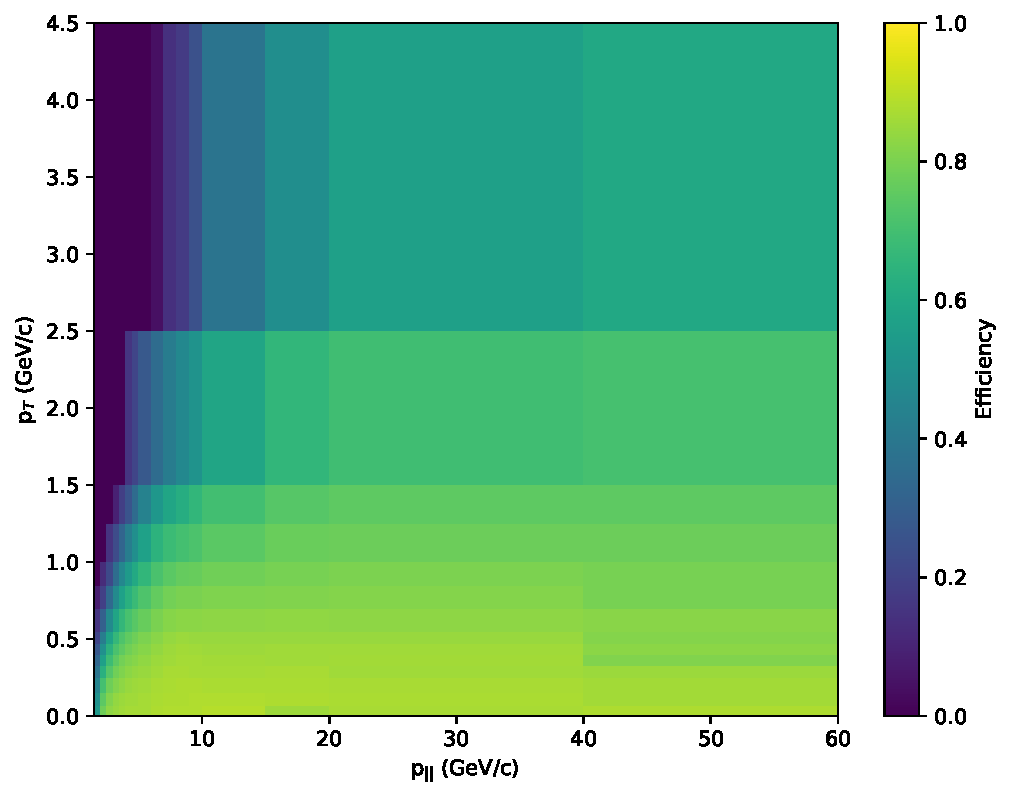
\includegraphics[width=0.62\textwidth]{MEFHC_5iter_xsec_eff_heatmap}
  \caption{Selection efficiency on the $(\pT,\pPar)$ truth grid. Efficiency is
  diagnostic only; OmniFold's miss treatment natively corrects acceptance
  (\S\ref{sec:method-algo}).}
  \label{fig:eff}
\end{figure}

\section{Results}
\label{sec:results}


The unfolded points of Fig.~\ref{fig:xsec} carry the bin errors stored with the unfolded histogram and its projections (\texttt{hXSec2D}, \texttt{hXSec\_pt}, \texttt{hXSec\_pz}); they are not drawn from the covariance of \S\ref{sec:systematics}.
The published points in its top panel carry the square root of the diagonal of the
published statistical covariance. The uncertainty budget of \S\ref{sec:systematics}
is shown in Fig.~\ref{fig:uqbands} and Table~\ref{tab:uq}.
Figs.~\ref{fig:ptslices}--\ref{fig:pzslices} carry statistical errors only,
as their captions specify.
% PHASE2 Q2, from the producers: plot_2d_threeway_fig13.py th2_to_array (hXSec2D.GetBinError) and paper_arrays
% (sqrt of StatOnlyCovariance diagonal); plot_2d_cross_section.py plot_1d_projection (hXSec_pt / hXSec_pz GetBinError).
% J3/J4 provisional (DECISION-20261018, packet J3: no claim change; the sentence states what the producers draw).

\subsection{Double-differential cross section}
\label{sec:results-xsec}
Figure~\ref{fig:xsec} shows the unfolded $d^{2}\sigma/(d\pT\,d\pPar)$ and its
1D projections. The total cross section is
\SI{\sigTwoD}{cm^2/nucleon} (published: \SI{\sigTwoDpaper}{cm^2/nucleon}).

The shapes are expected for CC-inclusive scattering at
$\langle E_\nu\rangle\sim\SI{6}{GeV}$. The $\pT$ projection vanishes at
$\pT=0$ and peaks broadly at $\pT\approx0.55$--$\SI{0.70}{GeV/c}$, reflecting
the $Q^{2}\lesssim\SI{1}{GeV^2}$ scale of few-GeV scattering through
$\pT^{2}\simeq Q^{2}\,E_\mu/E_\nu$, with $E_\mu/E_\nu\sim0.6$ for these forward
muons. It falls by more than two orders of magnitude toward the
\SI{4.5}{GeV/c} edge. The $\pPar$ projection rises from the
\SI{1.5}{GeV/c} threshold to a broad $\pPar\approx3$--$\SI{4.5}{GeV/c}$ maximum
(the NuMI medium-energy flux peak at $E_\nu\approx\SI{6}{GeV}$), then falls by two
orders of magnitude by $\pPar\approx\SI{20}{GeV/c}$. The
$\theta_\mu<20^{\circ}$ acceptance empties the 2D map's high-$\pT$, low-$\pPar$
corner (19 unreported diagonal cells; \S\ref{sec:method-binning}).



\begin{figure}[H]
  \centering
  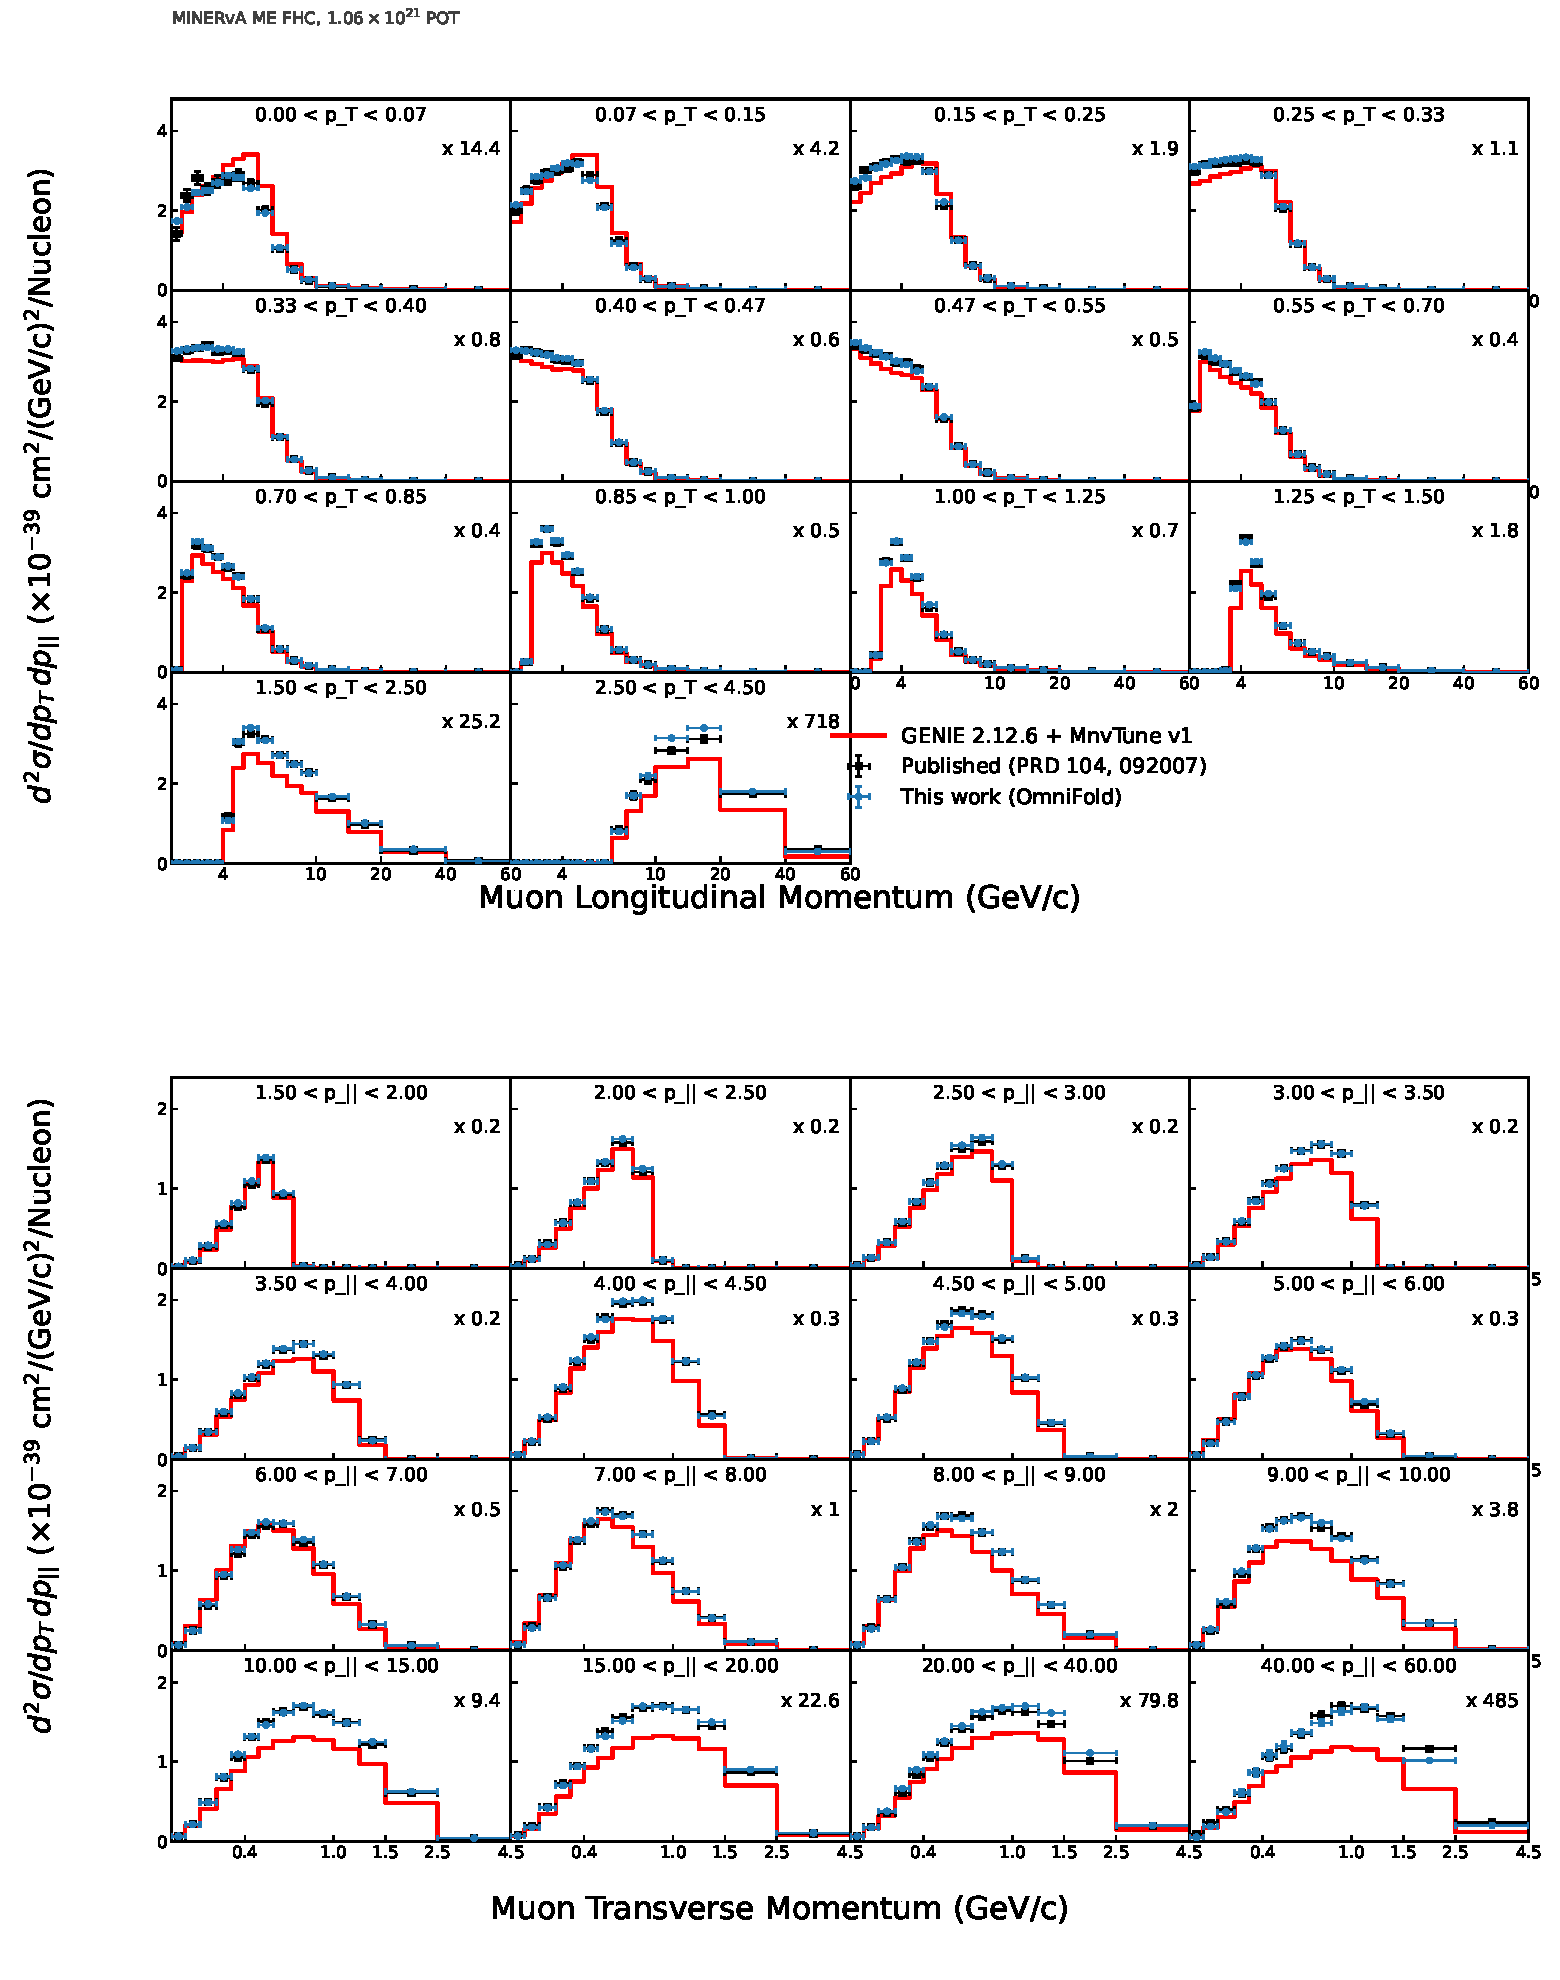
\includegraphics[width=0.62\textwidth]{MEFHC_5iter_fig13}\\
  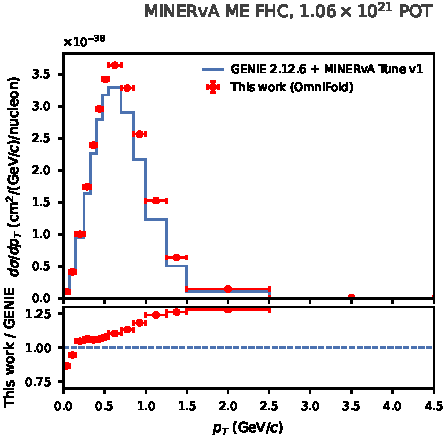
\includegraphics[width=0.49\textwidth]{MEFHC_5iter_xsec_proj_pt}
  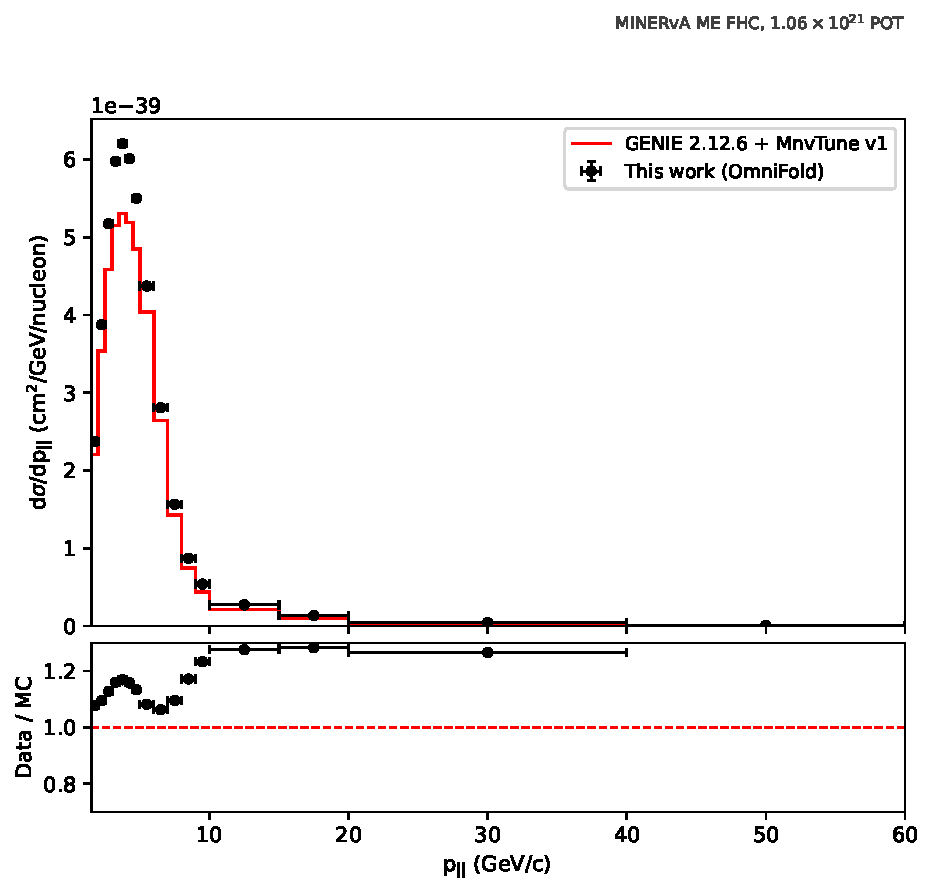
\includegraphics[width=0.49\textwidth]{MEFHC_5iter_xsec_proj_pz}
  \caption{Unfolded 2D cross section (top, Fig.~13 style) and its $\pT$/$\pPar$
  projections (bottom). The $\pT$ peak at ${\sim}\SI{0.6}{GeV/c}$ reflects
  the $Q^{2}\lesssim\SI{1}{GeV^2}$ momentum-transfer scale; the $\pPar$
  peak reflects the medium-energy flux maximum.}
  \label{fig:xsec}
\end{figure}


\subsection{Comparison to the published measurement}
\label{sec:results-compare}
The published and unbinned results share data and flux, detector, and generator
systematics, and their cross-covariance is not available. Every $\chi^{2}$ and
standardized difference here is therefore descriptive, shown for orientation only;
none is a calibrated goodness-of-fit test.

Over the 205 reported bins, the total cross section reproduces the published
result~\cite{MINERvA:2021owq} to \SI{1.1}{\percent} (ratio $\ratioTot$;
Table~\ref{tab:compare}). The median per-bin ratio is $\medianBinRatio$;
$\binsFive\%$ of bins agree within \SI{5}{\percent} and $\binsTen\%$ within
\SI{10}{\percent}. Indicative values of $\chi^{2}$ per reported bin use the
published covariance alone ($\chiPaper$) or the combined covariance, including
our uncertainty ($\chiCombined$); see \S\ref{sec:results-tension} for the former.

% chi^2 caveat, moved here from sec_systematics.tex (formerly \paragraph{$\chi^{2}$ caveat.}).
The combined paper$+$ours $\chi^{2}/\mathrm{ndf}=\chiCombined$ double-counts
shared flux/GENIE/MINOS systematics. The $\chi^{2}$ with our covariance alone is computed
only in its well-constrained subspace, with a truncated spectral pseudo-inverse.
We therefore quote the per-bin pulls, the truncated result and, as history, the
regularization scan of the exact-split cross-check on an earlier covariance, together,
rather than treating an unconstrained pseudo-inverse as a goodness-of-fit test on its
own (App.~\ref{sec:rank}).
% NR: the regularization scan was not recomputed for Q (no committed producer; rebuild REPORT §6).
% J3/J4 provisional (DECISION-20261018, packet C7: kept, labelled historical).
% plain-language pass (DECISION-20261018-joseph-plain-language-pass)

Per-bin differences standardized by the published uncertainty
(Fig.~\ref{fig:pull}) are centered (mean $\pullMean$), with RMS $\pullRMSr$
well inside the published uncertainties.
Figures~\ref{fig:ptslices}--\ref{fig:pzslices} compare our unfold with
\emph{simulated truth} in the published panel format. Published data do not
enter this data-versus-prior comparison.

\begin{table}[h]
  \centering
  \begin{tabular}{@{}lc@{}}
    \toprule
    Quantity (205 reported bins) & Value \\
    \midrule
    $\sigma_{\mathrm{tot}}(\mathrm{ours})/\sigma_{\mathrm{tot}}(\mathrm{paper})$ & $\ratioTot$ \\
    Median bin ratio (ours/paper) & $\medianBinRatio$ \\
    Bins within \SI{5}{\percent}/\SI{10}{\percent}/\SI{20}{\percent} & $\binsFive/\binsTen/\binsTwenty\,\%$ \\
    Indicative $\chi^{2}$/bin, paper covariance & $\chiPaper$ \\
    Indicative $\chi^{2}$/bin, paper $+$ ours & $\chiCombined$ \\
    Published-$\sigma$ standardized-difference mean / RMS & $\pullMean/\pullRMS$ \\
    \bottomrule
  \end{tabular}
  \caption{Agreement with arXiv:2106.16210. Per-bin differences standardized
  by published uncertainties (Fig.~\ref{fig:pull}) are sub-$1\sigma$;
  the $\chi^{2}$ values are descriptive.}
  \label{tab:compare}
\end{table}

\begin{figure}[H]
  \centering
  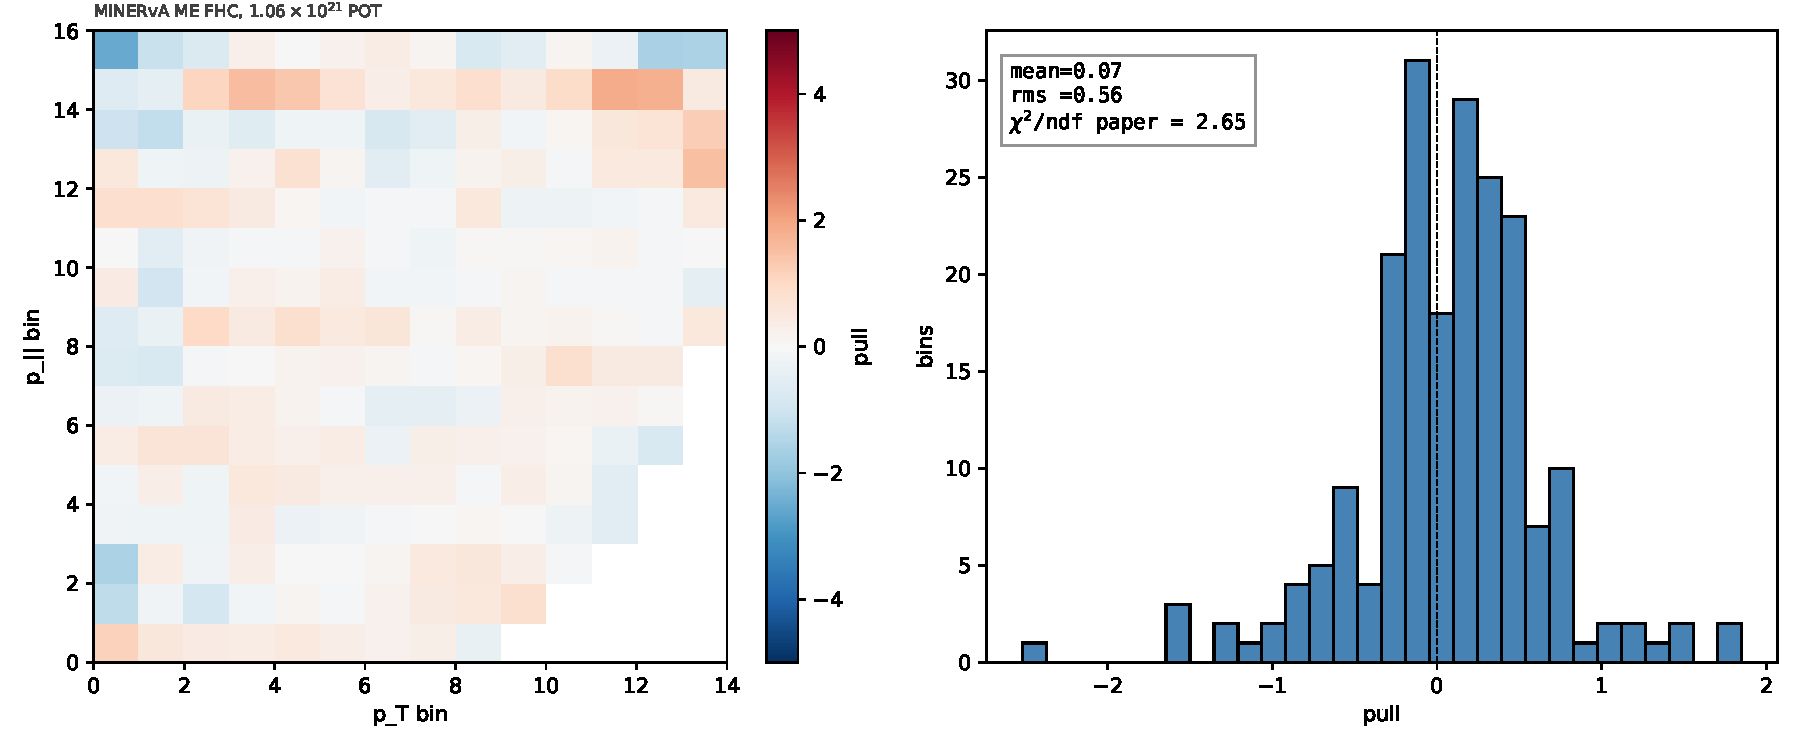
\includegraphics[width=0.7\textwidth]{MEFHC_5iter_pull_full}
  \caption{Per-bin standardized difference
  $(\mathrm{ours}-\mathrm{paper})/\sigma_{\mathrm{paper}}$ on the
  $14\times16$ grid and its distribution. It is descriptive, not a pull
  between independent results.}
  \label{fig:pull}
\end{figure}

\begin{figure}[H]
  \centering
  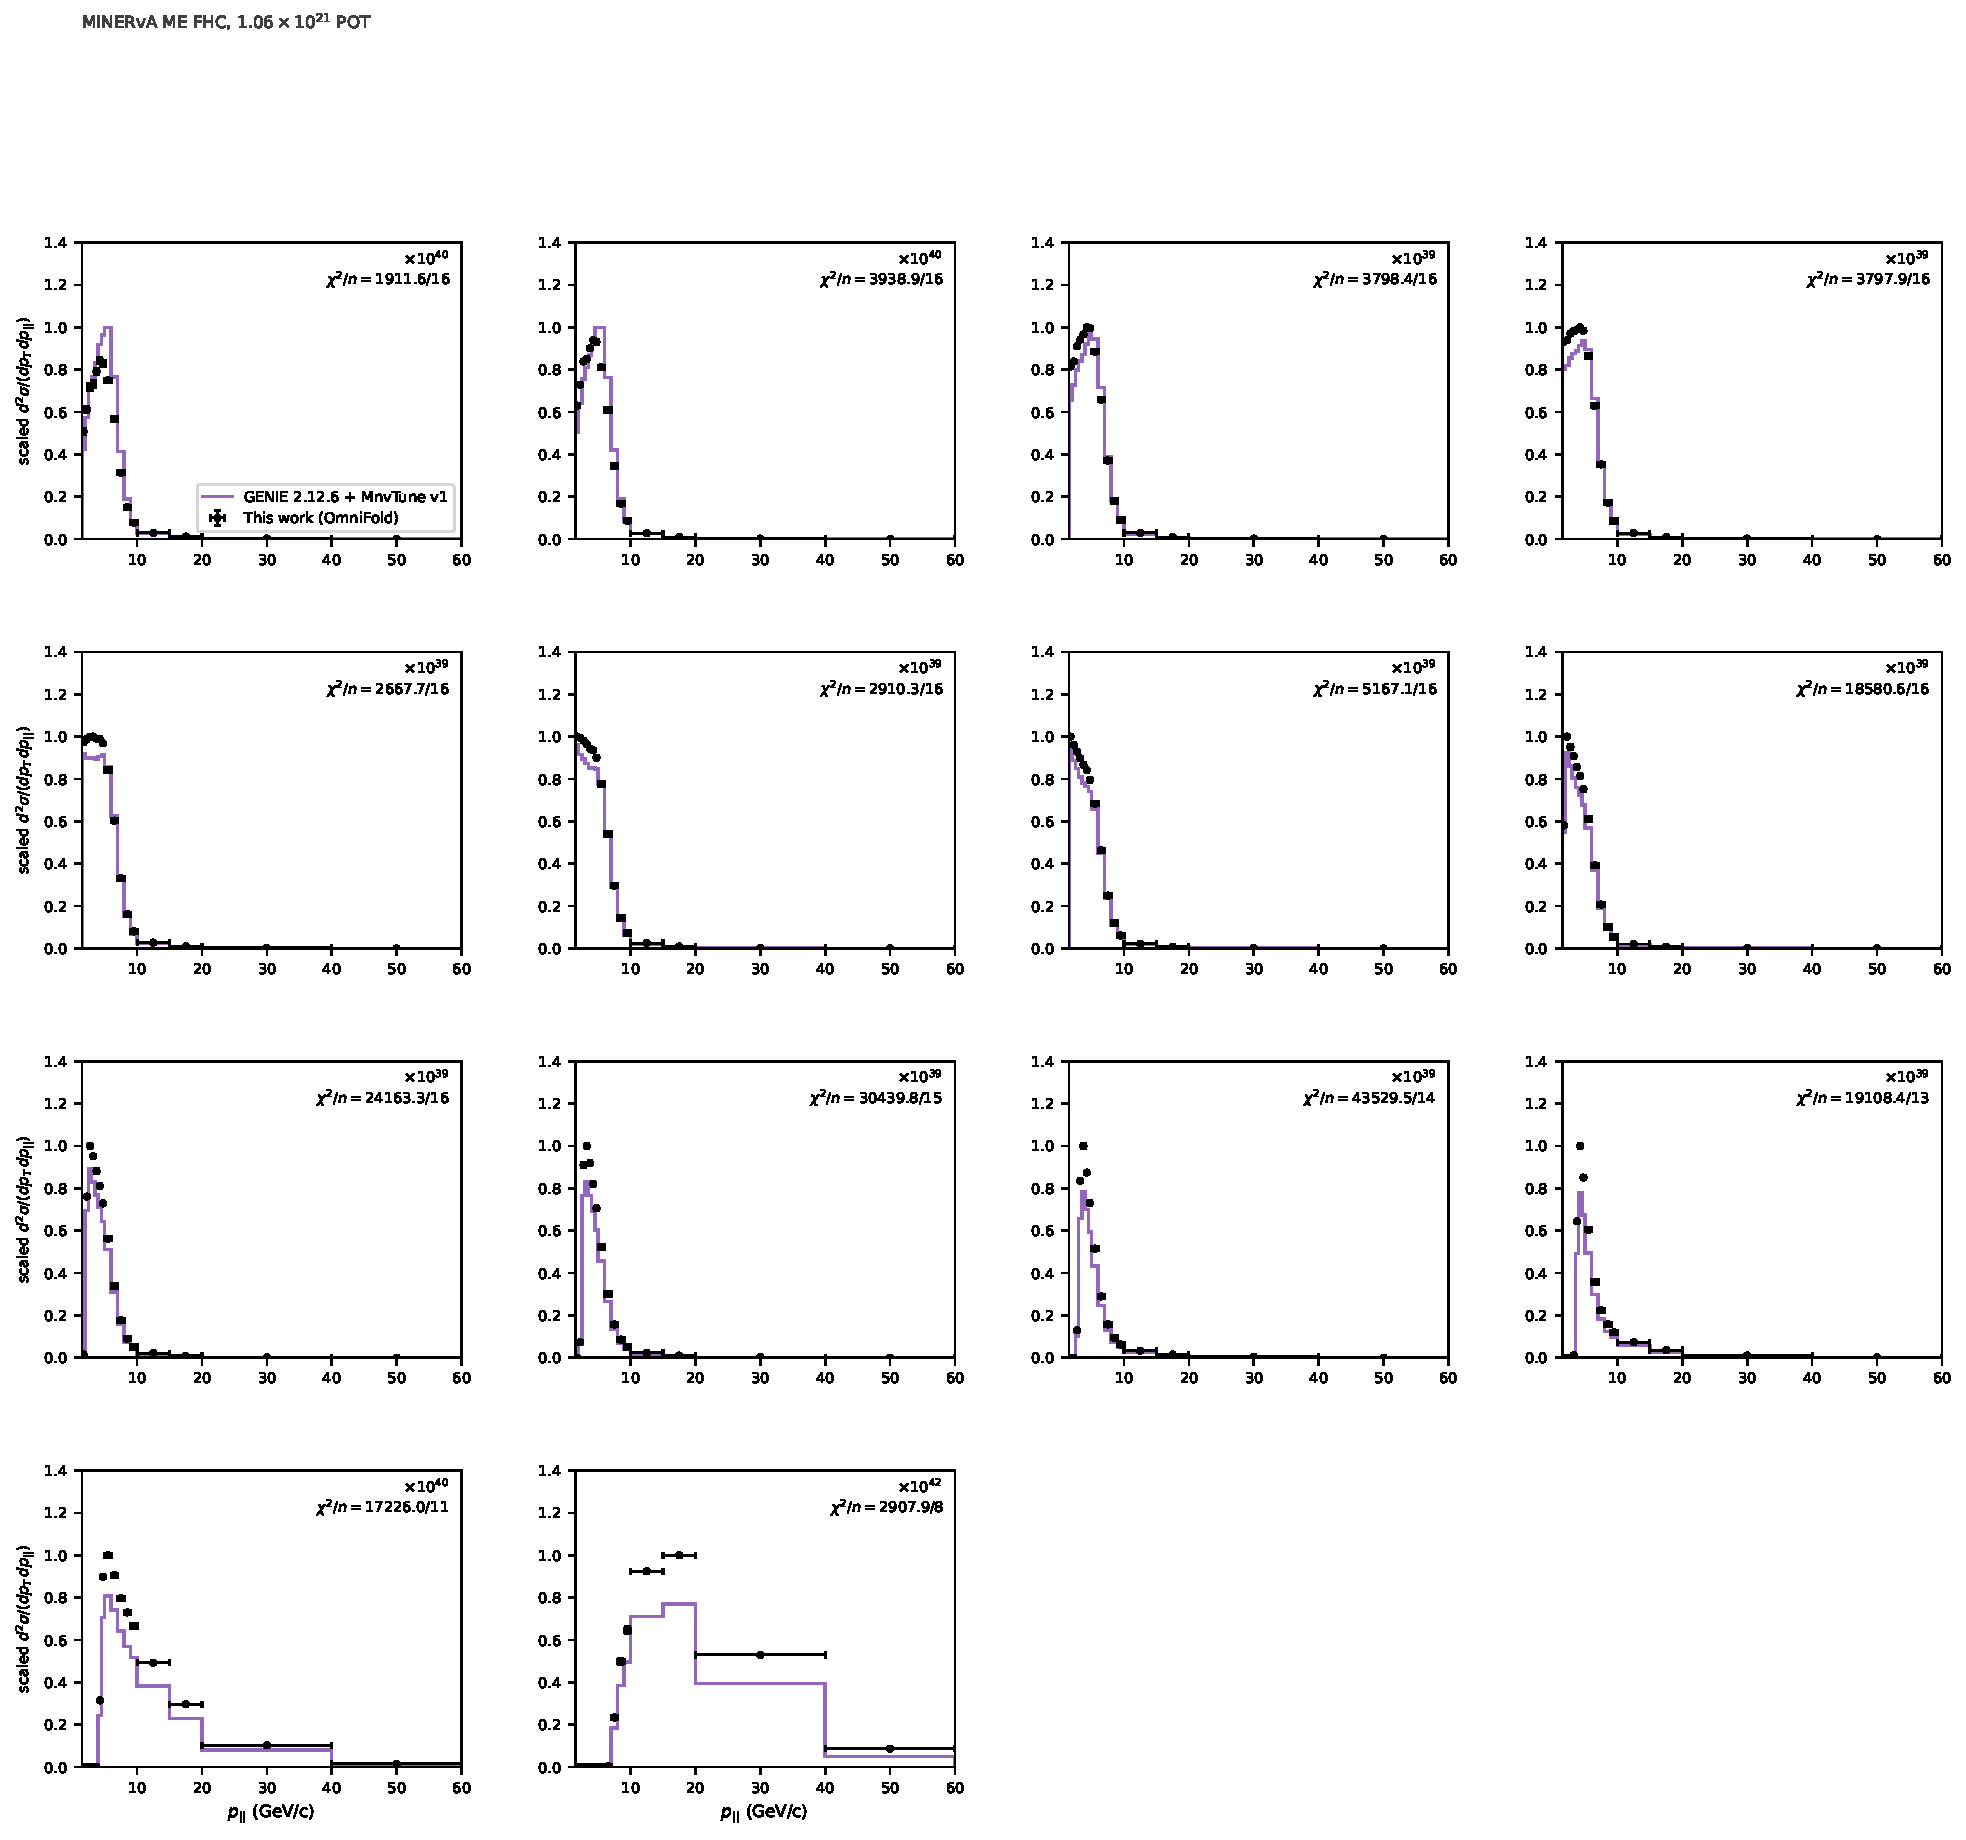
\includegraphics[width=0.99\textwidth]{MEFHC_5iter_xsec_paper_pt_slices}
  \caption{Unfolded cross section (points) and GENIE 2.12.6 $+$ MINERvA Tune~v1
  \emph{simulated truth} (histogram), sliced in $\pT$ versus $\pPar$.
  The histogram uses the analysis MC truth denominator with the unfolded
  result's flux, nucleon-count and efficiency normalization%
  % (\texttt{2d-unfolding/plot\_2d\_paper\_comparison.py} builds it from
  % \texttt{hOFTruthDenom2D}; listed in App.~\ref{app:codebase})
  . The curves differ only by data versus MC prior; no published measurement is read.
  Only the \emph{panel format} follows Fig.~13 of
  Ref.~\cite{MINERvA:2021owq}. Points carry statistical errors only;
  these alone enter the annotated per-panel $\chi^{2}$, a descriptive
  scale. Comparisons \emph{to the published data} appear in Fig.~\ref{fig:pull}
  (per-bin standardized differences), Table~\ref{tab:compare}, and
  Fig.~\ref{fig:model} (projections).}
  \label{fig:ptslices}
\end{figure}

\begin{figure}[H]
  \centering
  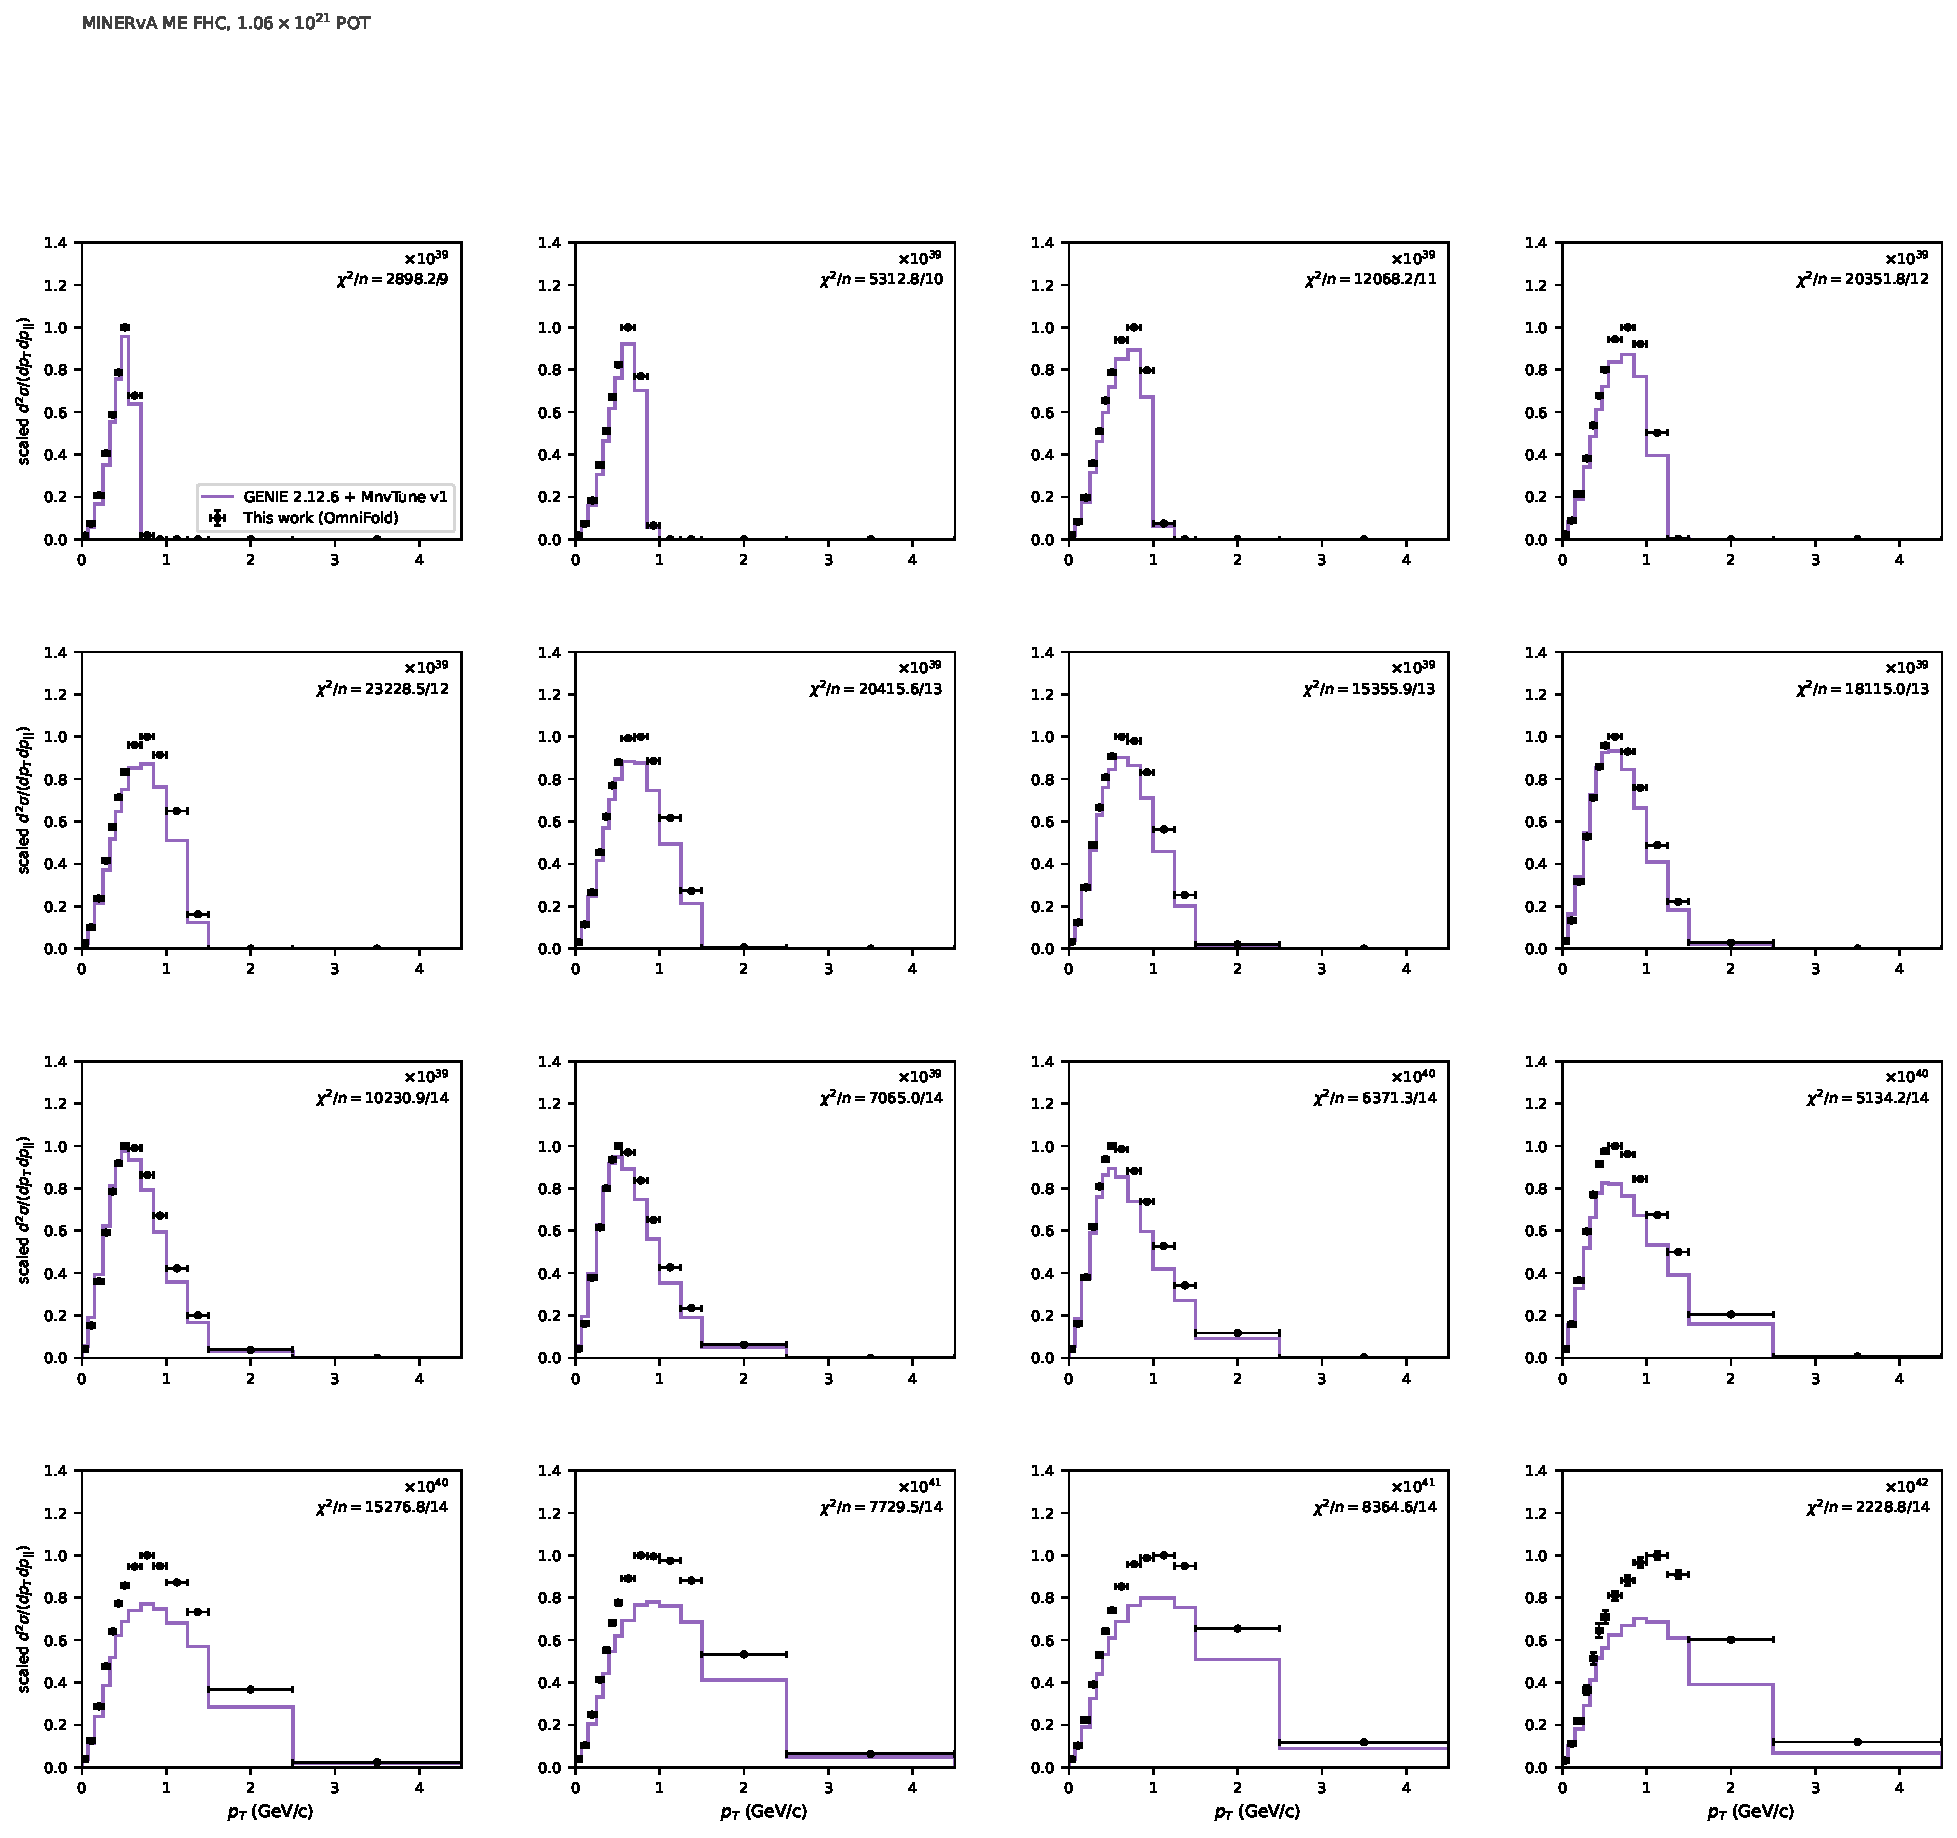
\includegraphics[width=0.99\textwidth]{MEFHC_5iter_xsec_paper_pz_slices}
  \caption{Unfolded versus simulated truth (Fig.~\ref{fig:ptslices}), sliced
  in $\pPar$ versus $\pT$. Statistical errors only; no published measurement
  is read.}
  \label{fig:pzslices}
\end{figure}

\subsection{Uncertainty budget}
\label{sec:results-uq}
Table~\ref{tab:uq} gives the budget over the 205 reported bins, constructed as
described in \S\ref{sec:systematics}. Our own combined budget, without the
published covariance, is comparable to the published total: its per-bin median is \SI{\uqMedian}{\percent} against
the published \SI{\uqPaper}{\percent}, and on the integrated cross section it is
\SI{\uqIntegral}{\percent} against the published \SI{\uqPaperIntegral}{\percent}
(the width-weighted total $\sigma$ of App.~\ref{sec:chisq}). Its largest band is the flux, as in
the publication (Fig.~\ref{fig:uqbands}); the systematic-universe block carries a median 0.87
of each bin's variance and 0.83 of the integral's, and the run-period block (\S\ref{sec:uq-combine}) raises the per-bin median from
\SI{\uqSFiveMedian}{\percent} to \SI{\uqMedian}{\percent}.
Its per-bin median is smaller than the published total's, and its integral larger; part of the
per-bin difference is the flux band (\SI{\fluxBand}{\percent} median, against
\SI{4.01}{\percent} for the published flux block; the public release does not
let us determine the origin of this difference, and our leading hypothesis, not
established, is the FHC-only constraint file).
Our flux band carries MAT's per-universe $\nu$--$e$ and inverse-muon-decay
constraint weights; an earlier version omitted them and quoted \SI{6.87}{\percent}
(App.~\ref{app:history}). The
statistical and ML blocks together contribute
under a tenth of the combined $\sqrt{\mathrm{Tr}\,C}$.
% J3/J4 provisional (DECISION-20261018, packet C2: median and integral; W3: D0; W5: the note keeps the 6.87 % history
% clause, pointing to App. history; W7: the flux sentence kept). Review m11: block_shares.universe is the median over cells
% of the per-cell share, not the share in the median bin. budget_Q.json.gz Q.median_pct (6.448),
% Q.integral_sigma_pct (4.755), S5_total.median_pct (6.041), block_shares.universe (0.871 per cell, median; 0.828 of the
% integral); \uqPaperIntegral 4.61 (values.tex). The sqrt(Tr) ratio (paper_ratios sqrt_trace_Q_over_sqrt_trace_TotalCovariance
% 1.071) also exceeds one and is not printed here.
% plain-language pass (DECISION-20261018-joseph-plain-language-pass). Printed pointer moved to this comment: the 6.87 % clause's
% (\texttt{KNOWN\_ISSUES.md} 95).
Every block is computed
with the LightGBM estimator of the quoted central value
(\S\ref{sec:method-config}), and the relative uncertainties divide by that
central value, the seed-42 central value of the universe sweep. Against the
exact-split cross-check the same combined covariance gives a combined median
of \SI{6.410}{\percent}.
% 2026-10-18: Q (adopted 2026-10-17): rebuild/outputs/outA/budget_Q.json.gz Q.median_pct 6.4479 vs E_U,
% Q_vs_EC.median_pct 6.4104 vs E_C.
% 2026-10-12: VL175 (state/2d-closeout/c04-repair/products/budget.json): 6.0898 % vs CV42, 6.0577 % vs E_C
% (computed from c04-repair/products/cov2d_blocks_205.npz; the same code on the VL172 export gives 6.8707/6.8269).
% Earlier source: ASSESSMENT-20261008-2d-estimator-pairing.md P14 (6.8707 % vs CV42, 6.8269 % vs E_C), reproduced
% by the review (e/recompute/rc_pairing.json.txt blocksum_median_rel_pct_den_exact_central); KNOWN_ISSUES 88.

\begin{table}[H]
  \centering
  \begin{tabular}{@{}lccc@{}}
    \toprule
    Component & $N$ & $\sqrt{\mathrm{Tr}\,C}$ & per-bin median rel.\ $\sigma$ \\
    \midrule
    ML noise (LightGBM training-seed settings) & 5 & \num{1.99e-41} & \SI{0.057}{\percent} \\
    Statistical (Poisson bootstrap) & 300 & \num{1.98e-40} & \SI{0.684}{\percent} \\
    Systematic (universe sweep $+$ \SI{1.4}{\percent} norm) & 43 bands${+}1$ & \num{2.73e-39} & \SI{5.969}{\percent} \\
    Run period & 3 & \num{8.34e-40} & \SI{2.137}{\percent} \\
    \textbf{Combined (block sum)} & --- & \num{2.87e-39} & \SI{6.448}{\percent} \\
    Paper TotalCov (reference) & --- & \num{2.68e-39} & \SI{\uqPaper}{\percent} \\
    % Q rows: rebuild/outputs/outA/budget_Q.json.gz {c08,stat,universe,C_PL,Q}.{sqrt_trace,median_pct};
    % paper: paper_ratios.paper_sqrt_trace_TotalCovariance_205 (2.676e-39). Row labels:
    % J3/J4 provisional (DECISION-20261018, packet W3: D0, D5; W10: block names as in the text).
    \bottomrule
  \end{tabular}
  \caption{2D uncertainty budget over 205 reported bins. Each component has
  a $205\times205$ covariance matrix $C$; $\sqrt{\mathrm{Tr}\,C}$ gives its
  absolute per-bin uncertainties in quadrature. The flux band carries MAT's
  constraint weights. The systematic row holds 43 bands of the July sweep (44 bands,
  187 universes) plus the normalization; the ML row has five training-seed settings and
  the run-period row three run periods. Our combined median relative
  uncertainty (\SI{6.448}{\percent}) is below the published total
  (\SI{\uqPaper}{\percent}).}
  \label{tab:uq}
\end{table}
\subsection{Anatomy of the $\chi^{2}=\chiPaper$ tension}
\label{sec:results-tension}
Using the published uncertainties as a descriptive scale, the central values
have pull RMS $\pullRMS$ (a diagonal-only $\chi^{2}/\mathrm{ndf}$ would be
$0.32$), while the full paper-covariance distance is $\chiPaper$ per bin:
an $8\times$ inflation living entirely in the off-diagonal structure of the
published covariance. It is \emph{shape}, not normalization
($\chi^{2}_{\mathrm{norm}}=0.06$ vs $\chi^{2}_{\mathrm{shape}}=544$). The
eigenmode decomposition (Fig.~\ref{fig:tension}) spreads it over many modes,
the largest with paper-covariance-standardized components of magnitude about
$4$--$5$; the 10 smallest-$\lambda$ modes carry \SI{9.5}{\percent}, two of the
five largest contributors lie in the smallest-$\lambda$ tenth, and keeping the
73 best-measured directions gives $0.81$. The four leading modes in the
highest-$\pPar$ bins are all poorly determined directions
($\lambda/\lambda_{\max}\lesssim4\times10^{-9}$); the two leading
moderate-$\lambda$ modes lie at low-to-moderate $\pT$, below the highest $\pPar$
(Fig.~\ref{fig:tensionmodes}). No single $\pT$ or $\pPar$
band carries more than \SI{15}{\percent} of the total. The GBDT estimator gives
a $\sim1$-unit methodological band (the exact-split cross-check
$\chiPaperExact$, HistGBT $2.70\pm0.04$, LightGBM seeds 1--10 2.64--2.75).
For the exact-split cross-check the distance is larger and differently
distributed: magnitude-$5$--$6$ components in moderate-$\lambda$ modes on the
low-$\pT$ cross-section peak ridge, \SI{3}{\percent} from the 10
smallest-$\lambda$ modes and $1.42$ from the 73 best-measured directions
(App.~\ref{sec:tension}). Iteration-count effects are negligible: $5\to10$
iterations move the LightGBM (seed~1) distance by $+0.01$.
% 2026-10-11: LightGBM seed-42 values from diagnose_tension.py at e1216e9c,
% docs/orchestration/receipts/2d-lgbm42-20261011/tension_report.txt; the exact-split control
% (tension_report_exact_control.txt) reproduces 0.37 (0.366), 10x, 3 %, 1.42 and 0.10/750.
See App.~\ref{sec:tension} for the full treatment and
Figs.~\ref{fig:tension}--\ref{fig:tensionmodes} for eigenmode-localization maps.
% NOTE (2026-10-11): the exact-split cross-check's 3.66 is \chiPaperExact; \chiPaper is now the LightGBM 2.65.

\begin{figure}[H]
  \centering
  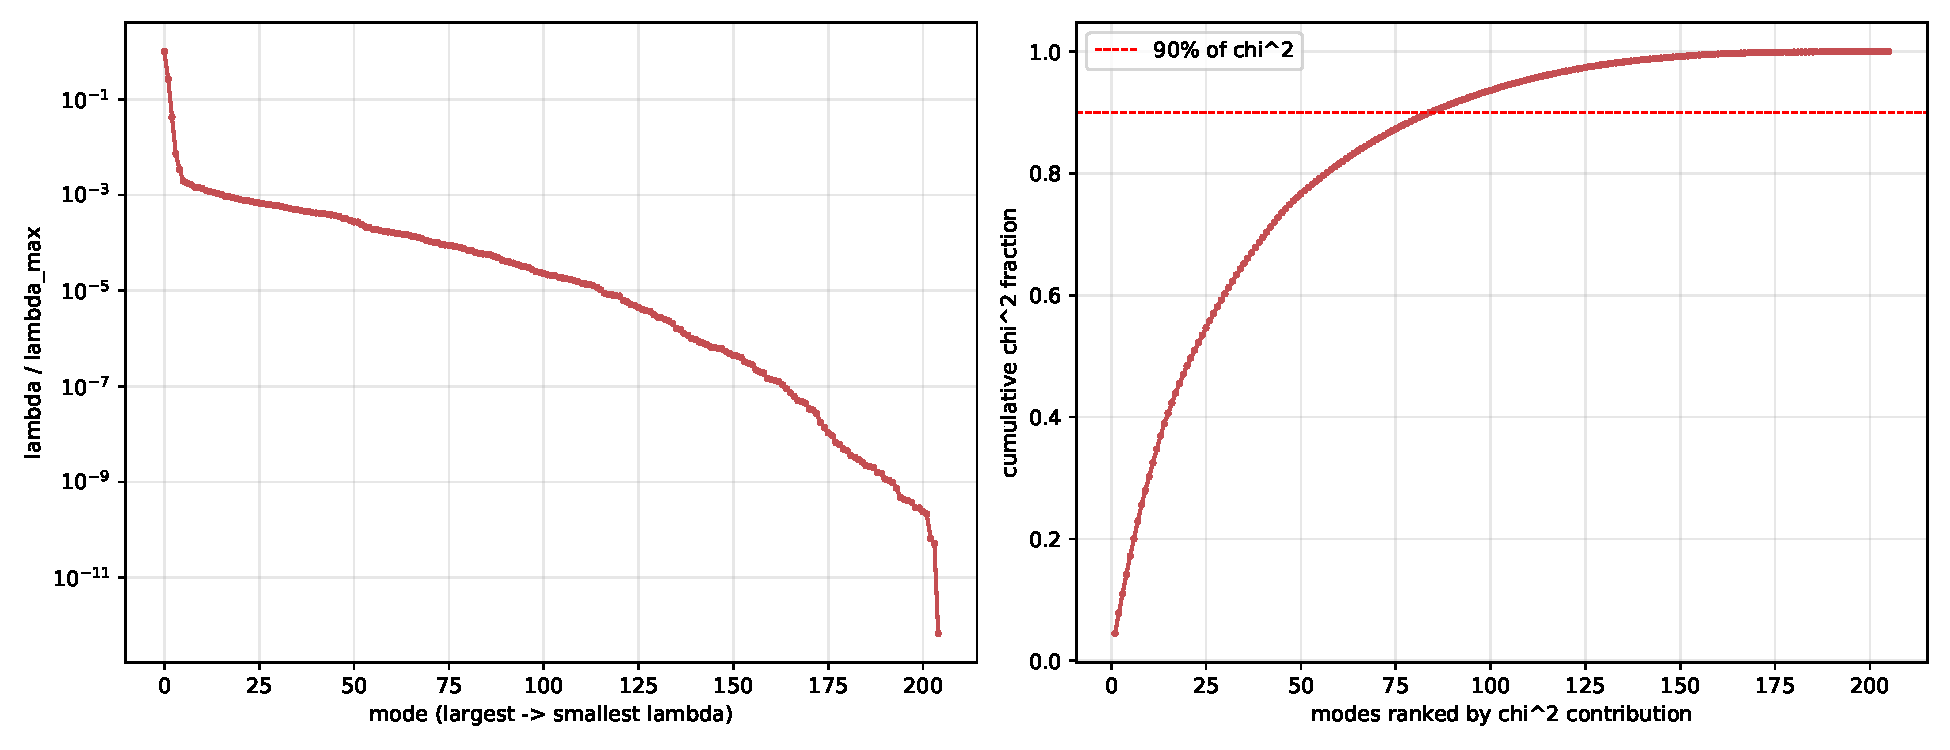
\includegraphics[width=0.49\textwidth]{tension_spectrum}
  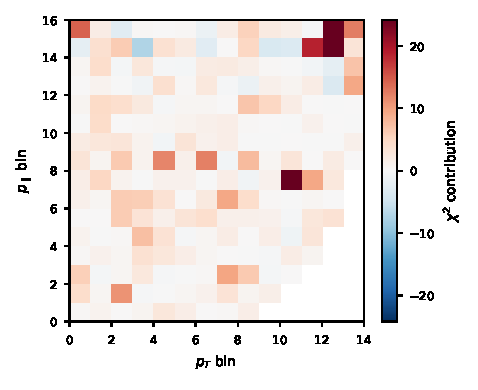
\includegraphics[width=0.49\textwidth]{tension_chi2_map}
  \caption{Tension anatomy: eigenvalue spectrum with cumulative $\chi^{2}$ (left)
  and the per-bin $\chi^{2}$-contribution map (right).}
  \label{fig:tension}
\end{figure}

\begin{figure}[H]
  \centering
  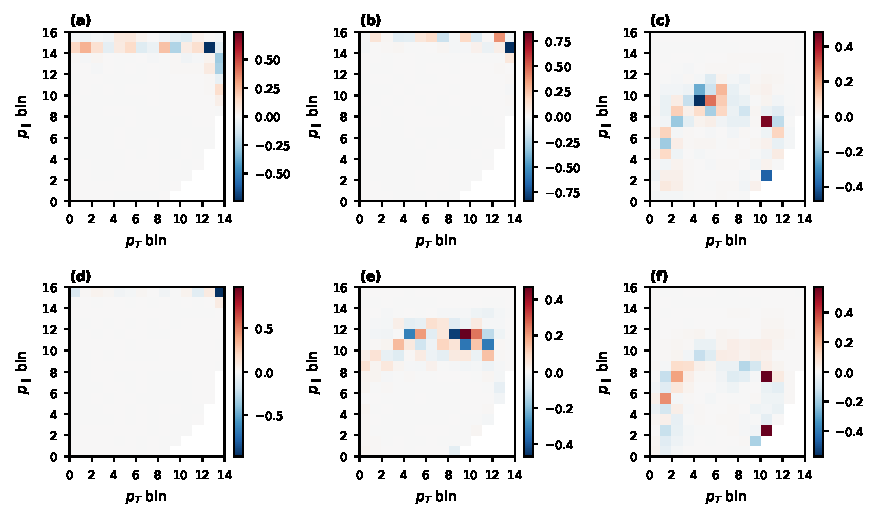
\includegraphics[width=0.9\textwidth]{tension_mode_maps}
  \caption{Leading tension-carrying eigenmodes of the published covariance
  in bin space, for the LightGBM central value. Four of the six, all
  smallest-$\lambda$ directions, concentrate in the highest-$\pPar$ bins; two
  moderate-$\lambda$ modes lie at low-to-moderate $\pT$.}
  \label{fig:tensionmodes}
\end{figure}

\subsection{Comparison to GENIE MINERvA Tune v1}
\label{sec:results-model}
GENIE 2.12.6~\cite{Andreopoulos:2009rq} MINERvA Tune v1 under-predicts the total
by $\sim\SI{9}{\percent}$ ($\sigma_{\mathrm{tune}}/\sigma_{\mathrm{data}}=0.91$),
concentrated in the low-$\pT$ peak. The ancillary prediction is compared with
both the published data and our result in Fig.~\ref{fig:model}. The data
covariance strongly disfavors the tune ($\chi^{2}/\mathrm{ndf}$: data vs tune
$33.0$, ours vs tune $29.8$; $26.5$ for the exact-split cross-check). Our unfold tracks the data far more closely than
the model does (Fig.~\ref{fig:modelmaps}).
The published analysis~\cite{MINERvA:2021owq} also compares with
NuWro~\cite{Golan:2012wx}, GiBUU~\cite{Buss:2011mx} and NEUT~\cite{Hayato:2009zz}.
OmniFold's per-event reweighted truth ensemble can be compared with any
such prediction in \emph{any} projection of classifier features without
re-unfolding. Adding an observable outside that space is a new
unfold, not a projection: the 3D extension (\S\ref{sec:3d}) adds $\Eavail$ as a
classifier feature and is re-unfolded accordingly.

\begin{figure}[H]
  \centering
  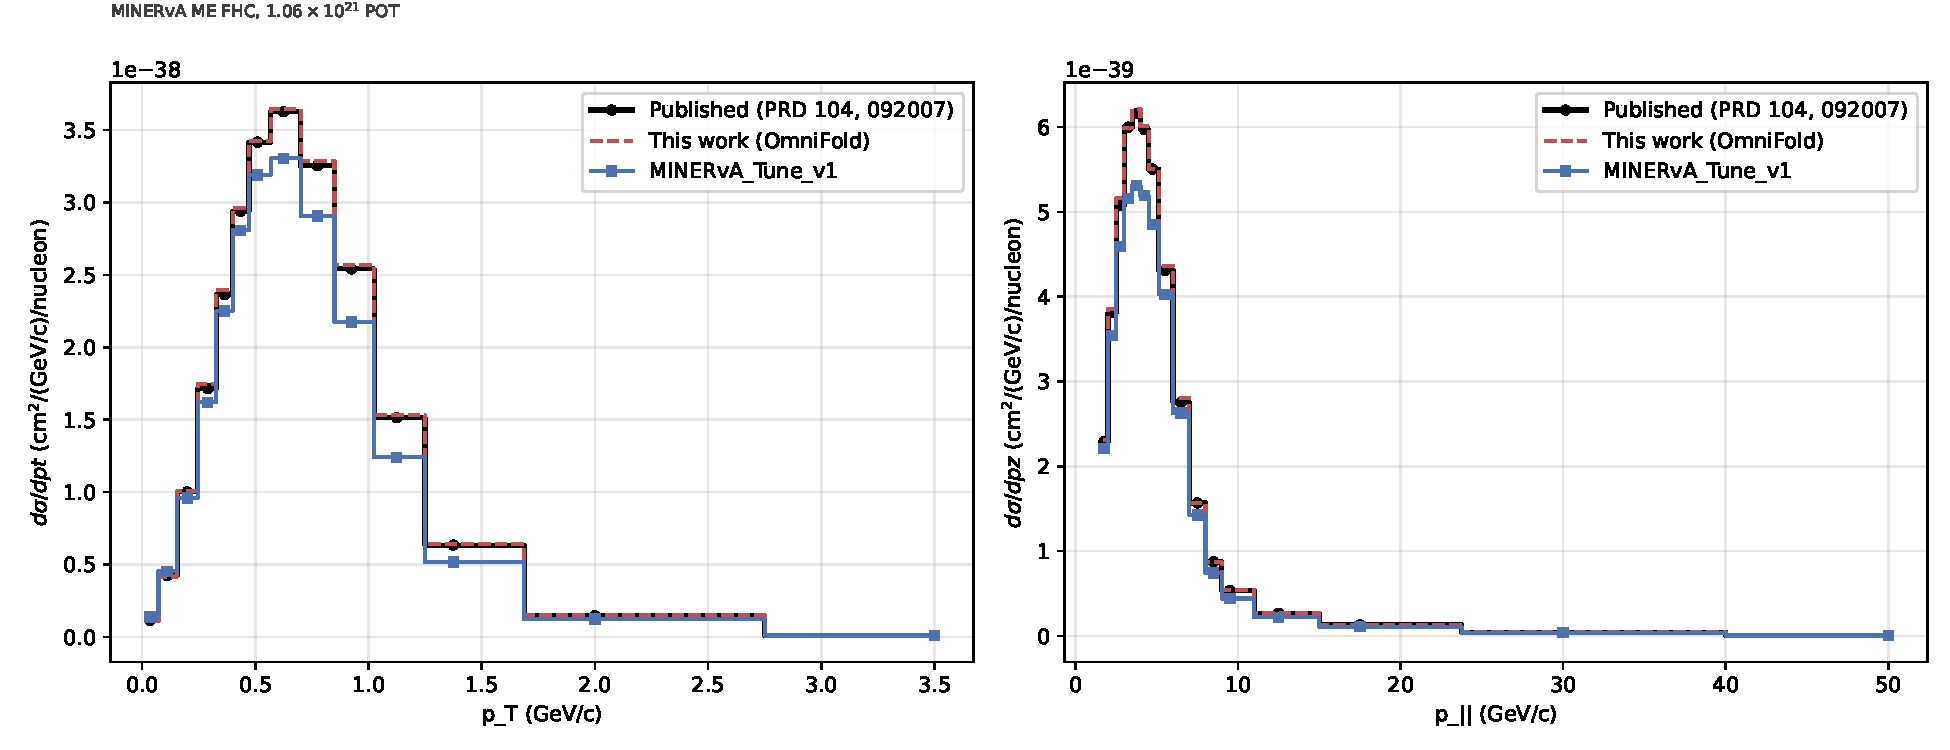
\includegraphics[width=0.85\textwidth]{model_comp_projections}
  \caption{Our result (dashed) on top of the published data (black); MINERvA
  Tune v1 (orange) dips below in the peak.}
  \label{fig:model}
\end{figure}

\begin{figure}[H]
  \centering
  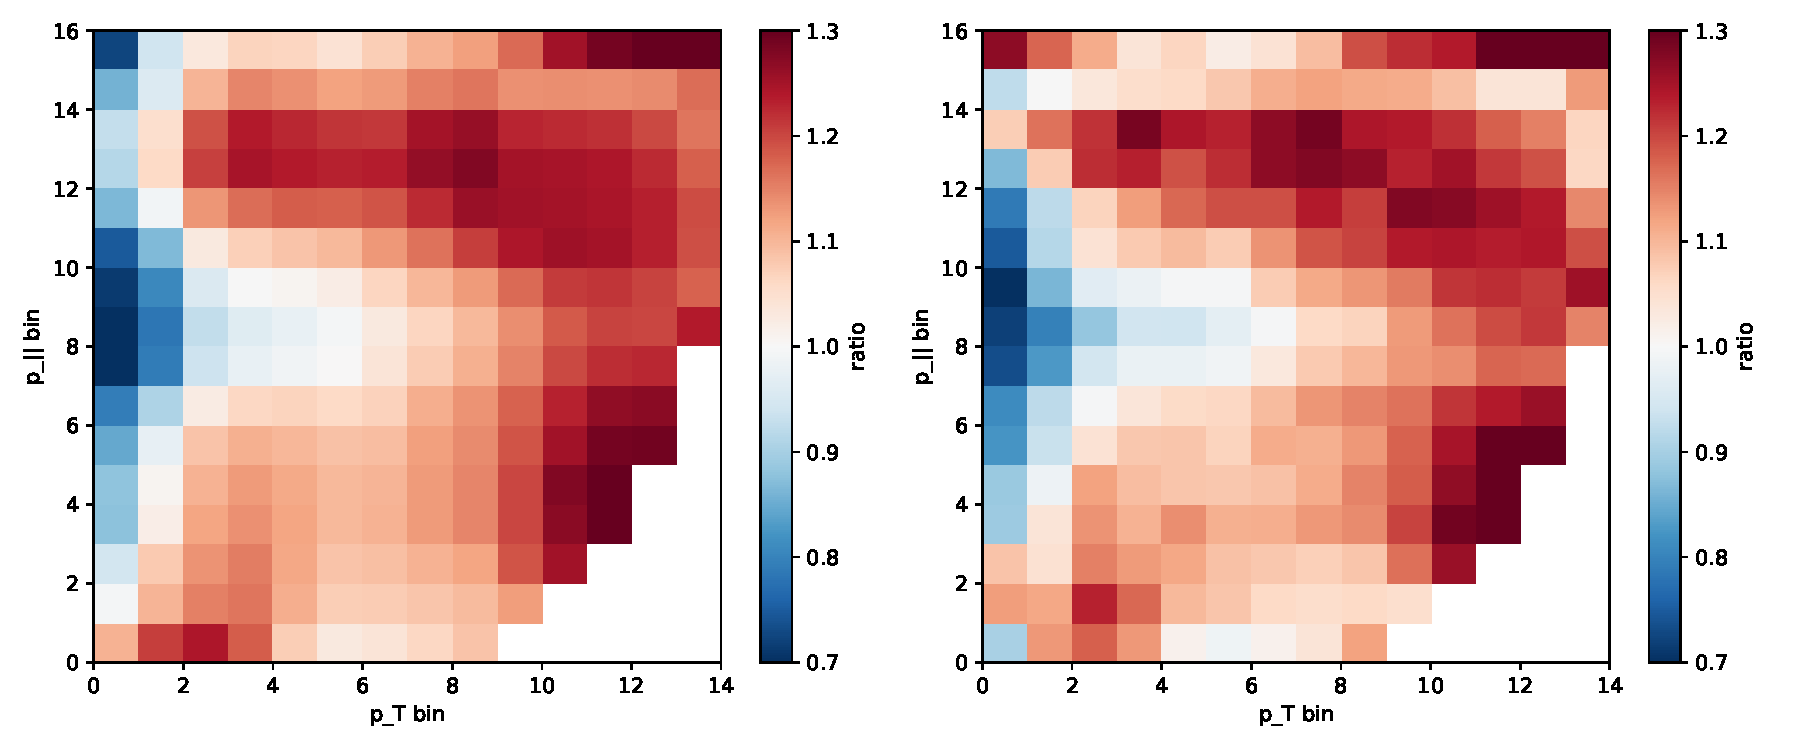
\includegraphics[width=0.9\textwidth]{model_comp_ratio_maps}
  \caption{Bin-by-bin ratios to MINERvA Tune~v1 on the $(\pT,\pPar)$ grid:
  ours/Tune~v1 (left) and published data/Tune~v1 (right), with common colour
  scale $0.7$--$1.3$
  % (\texttt{2d-unfolding/compare\_to\_models.py}; listed in App.~\ref{app:codebase})
  (only this caption labels the panels; they have no printed titles).
  Neither map uses published data as its denominator or is flat near unity.
  Both show the same tune deficit, above unity over most of the plane and
  dipping below at the lowest $\pT$. The close maps reflect that our result departs from
  the tune in the same places and by similar amounts as the published data. Direct comparison with
  published data uses Table~\ref{tab:compare}'s median bin ratio and
  Fig.~\ref{fig:pull}'s residual map.}
  \label{fig:modelmaps}
\end{figure}

\section{Higher-dimensional extensions: available energy and momentum transfer}
\label{sec:3d}

Unbinned OmniFold adds an observable by adding a column to the step-1/step-2
classifiers, without an explicit migration matrix or per-bin response tensor.
It avoids the combinatorial binning penalty of matrix unfolding but is not free
of a dimensional cost: classifier training, acceptance/support coverage, sample
sparsity and uncertainty quantification become more demanding as observables
are added. The absence of a practical D'Agostini
IBU analog is the primary methodological motivation.
We extend the measurement to
$d^{3}\sigma/(d\pT\,d\pPar\,d\Eavail)$ with available energy as a third axis.

MINERvA has published binned triple-differential results
(Fig.~\ref{fig:landscape}, Table~\ref{tab:landscape}), including recent comparisons
between low- and medium-energy beams~\cite{MINERvA:2026qeleme}. The latter measure
$\pT$, $\pPar$, and available recoil energy for a quasielastic-like signal, for
which the available energy is the sum of proton kinetic energies. This differs
from the inclusive signal and species-dependent energy definition used here.
Our distinction is the unbinned, simultaneous CC-inclusive scalar formulation
extended to three, four and five recorded observables, not multidimensionality
by itself.

\begin{figure}[H]
  \centering
  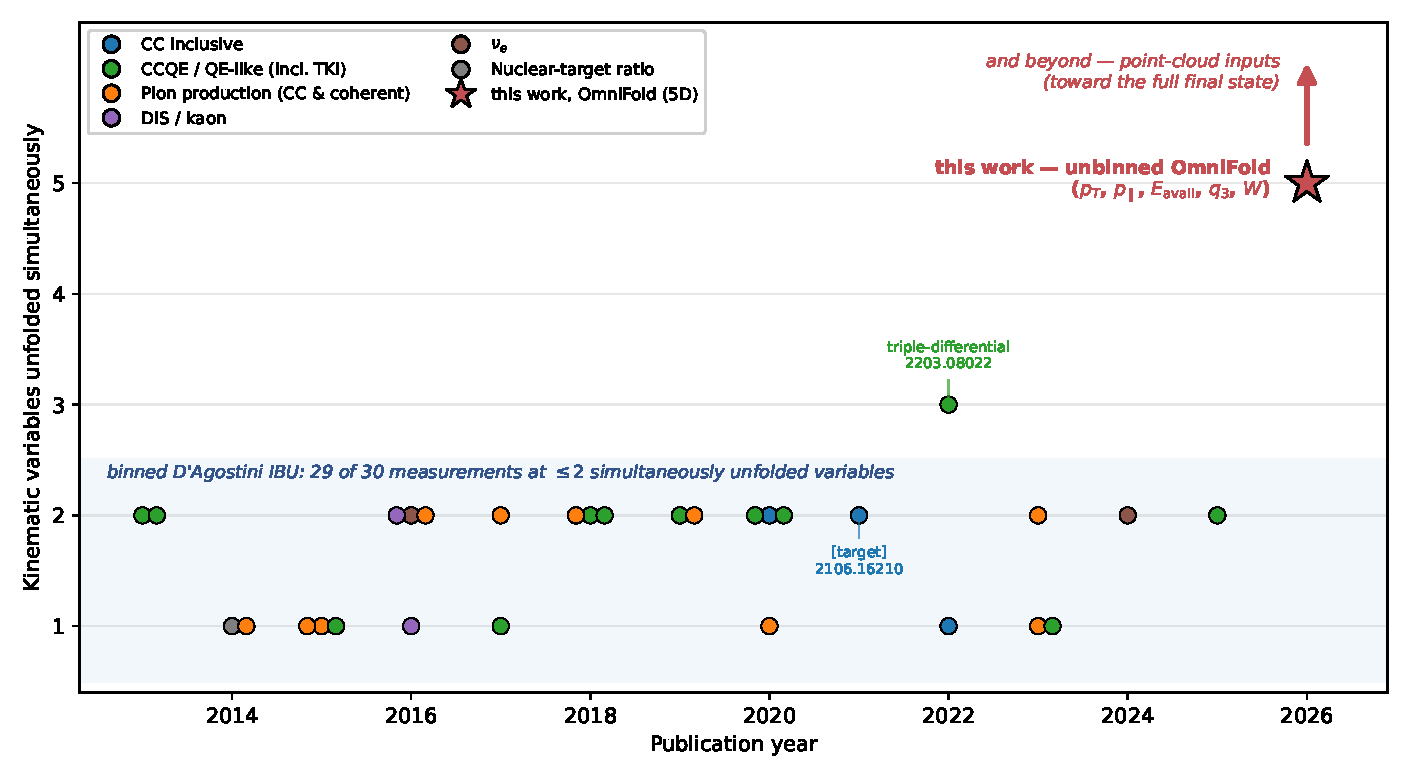
\includegraphics[width=0.97\textwidth]{minerva_unfolding_landscape}
  \caption{Number of kinematic variables unfolded \emph{simultaneously} in
  surveyed MINERvA differential cross-section measurements, by year, colored by channel
  (a double-differential $d^{2}\sigma/dx\,dy$ counts as two).
  Prior results use explicit binned unfolding, including a triple-differential
  quasielastic-like measurement; this work extends an unbinned CC-inclusive
  scalar unfold to five recorded observables.
  Source: the MINERvA data-release page and the cited publications. The plotted
  inventory runs through 2025; newer measurements are listed in
  App.~\ref{app:landscape}. Classification uses each analysis's headline
  differential result; flux, reconstruction, generator-tuning and
  total-only entries are excluded.}
  \label{fig:landscape}
\end{figure}

\subsection{Operational definition and provenance}
\label{sec:3d-method}
\label{sec:eavail-definition}
Truth available energy follows the code; ``low-recoil convention'' is
shorthand. In MeV, \texttt{CVUniverse::GetEAvailableTrue()} implements
\begin{equation}
 E_{\rm avail}^{\rm true}=
 \sum_{p}(E-938.27)
 +\sum_{\pi^\pm}(E-135)
 +\sum_{\pi^0}E
 +\sum_{\gamma}E .
 \label{eq:eavail-implemented}
\end{equation}
Protons and charged pions contribute the indicated kinetic-energy-like terms;
neutral pions and photons contribute total energy. All other final-state species
contribute zero, including neutrons, the primary muon, secondary $e^\pm$,
neutrinos, kaons, antiprotons, strange baryons, other mesons and nuclear-remnant
records. Reconstructed available energy
is the MAT calorimetric quantity
\begin{equation}
 E_{\rm avail}^{\rm reco}=1.17\left[(E_{\rm blob}^{\rm tracker}
 -E_{\mu\text{-fuzz}}^{\rm tracker})+(E_{\rm blob}^{\rm ECAL}
 -E_{\mu\text{-fuzz}}^{\rm ECAL})\right],
 \label{eq:eavail-reco-implemented}
\end{equation}
implemented by \texttt{CVUniverse::NewEavail()}; the code applies no final
non-negative clamp.

Both functions were inherited from MAT-MINERvA rather than selected in this
analysis.  Agreement with a published convention is therefore a defence of the
inherited position, not its provenance, and there is no unique published
$E_{\rm avail}$ definition.  Rodrigues \emph{et al.}~\cite{MINERvA:2016lowrecoil}
give a closed five-species list of proton and charged-pion kinetic energy plus
$\pi^0$, electron and photon total energy.  Equation~\eqref{eq:eavail-implemented}
matches four of those five species and excludes secondary $e^\pm$.
The later Ascencio \emph{et al.}~\cite{MINERvA:2022incl} definition is open and
includes other final-state particles except neutrons, subtracting a nucleon
mass for strange baryons. It therefore includes species our closed list omits.
The charged-pion term in Rodrigues and in Henry/Su \emph{et al.}
Eq.~4~\cite{MINERvA:2023avz} is kinetic energy; the
\texttt{minerva-ml} implementation discussed in \S\ref{sec:pet-gregor} instead
uses charged-pion total energy.  We therefore do not claim generically to
``match the published definition.''

Production subtracts the inherited constant
\SI{135}{MeV} per charged pion rather than the physical charged-pion mass of
approximately \SI{139.57}{MeV}; this was not corrected. The effect is measured
but has not been assessed against the adopted scalar-5D projection. Its
materiality is not established, and this note does not call it immaterial.
% This note neither applies the six-site correction nor triggers a rerun.

The reconstructed coordinates share inputs. In units with $c=1$, the implemented definitions (with reconstructed muon quantities) are
\begin{align}
 E_\nu^{\rm reco} &= E_\mu+q_0^{\rm reco},\nonumber\\
 Q^2_{\rm reco} &= \max\!\left\{0,\,
 2E_\nu^{\rm reco}(E_\mu-p_\mu\cos\theta_\mu)
 -m_\mu^2\right\},\nonumber\\
 q_3^{\rm reco} &= \sqrt{Q^2_{\rm reco}+(q_0^{\rm reco})^2},\nonumber\\
 W^{\rm reco} &= \sqrt{\max\{0,M^2+2Mq_0^{\rm reco}-Q^2_{\rm reco}\}},
 \label{eq:shared-reco-inputs}
\end{align}
where $m_\mu^2=E_\mu^2-p_\mu^2$ and $M$ is the average nucleon mass. The recoil-energy estimate $q_0^{\rm reco}$ differs from the tracker-plus-ECAL available energy $\Eavail^{\rm reco}$; truth $\Eavail$ also omits energy carried by species such as neutrons and is not the full energy transfer. Thus five recorded coordinates do not establish five independently constrained physical directions. Adding a coordinate, supplying a new detector input, and resolving a new truth direction are separate questions.
% Source: CVUniverse.h, NewEavail(), RecoQ3(), RecoW(), GetEAvailableTrue().


\paragraph{Pipeline and binning.}
The event loop evaluates both accessors over all twelve ME~FHC playlists,
carrying $\Eavail$ alongside $\pT$/$\pPar$. The 2D driver uses a three-column
feature stack $(\pT,\pPar,\Eavail)$; extraction uses the 3D Jacobian
$\Delta\pT\,\Delta\pPar\,\Delta\Eavail$. Flux $\Phi$ remains applied per
$\pT$ (broadcast over $\pPar$ and $\Eavail$). The $\Eavail$ binning
$[0,0.1,0.2,0.4,0.8,1.5,3.0,100]\,\si{GeV}$ ends in a wide catch bin to
capture the full CC-inclusive recoil tail in the $\Eavail$-marginal. Global
OmniFold completeness is $c=1.0000$, as in 2D.

\subsection{The available-energy spectrum}
\label{sec:3d-spectrum}
The unfolded $d\sigma/d\Eavail$, the 1D projection
of the 3D result
(Fig.~\ref{fig:eavail}), falls monotonically from
\SI{2.19e-38}{cm^2/GeV/nucleon} at the low-recoil peak to
\SI{6.8e-41}{} in the catch bin, the expected CC-inclusive shape with most
of the rate at $\Eavail\lesssim\SI{0.8}{GeV}$.

\begin{figure}[H]
  \centering
  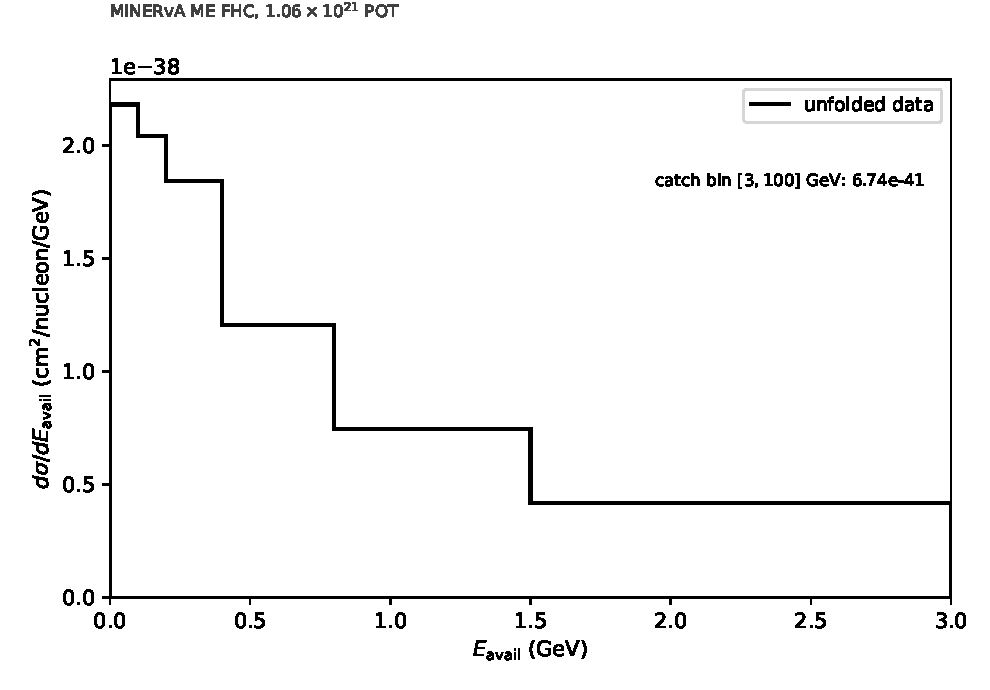
\includegraphics[width=0.66\textwidth]{eavail_spectrum}
  \caption{Unfolded $d\sigma/d\Eavail$, the 1D projection of the 3D measurement.
  The wide $[3,100]\,\si{GeV}$ catch bin is excluded from the axis; its value is annotated.}
  \label{fig:eavail}
\end{figure}

\subsection{Validation against the 2D measurement}
\label{sec:3d-anchor}
Marginalizing over $\Eavail$ must reproduce the 2D result of
\S\ref{sec:results}, our validation anchor in the absence of a directly matched
published CC-inclusive 3D reference for this signal and phase space.
The \emph{normalization} agrees closely, with total $\sigma$ at
$+\SI{0.95}{\percent}$ and median per-bin marginal/2D ratio $1.0016$.
The \emph{shape} agrees less closely. Using published covariance gives an indicative distance
$\chi^{2}/\mathrm{ndf}=4.98$,
above the frozen 2D values ($3.66$ default, $2.65$ LightGBM-CV), driven by
$\sim\SI{4.4}{\percent}$ per-bin scatter introduced by the third axis in the
$(\pT,\pPar)$ marginal (Fig.~\ref{fig:eavail-marg}).
Shared data and unavailable cross-covariance prevent interpreting this number
as a calibrated goodness-of-fit statistic.

\begin{figure}[H]
  \centering
  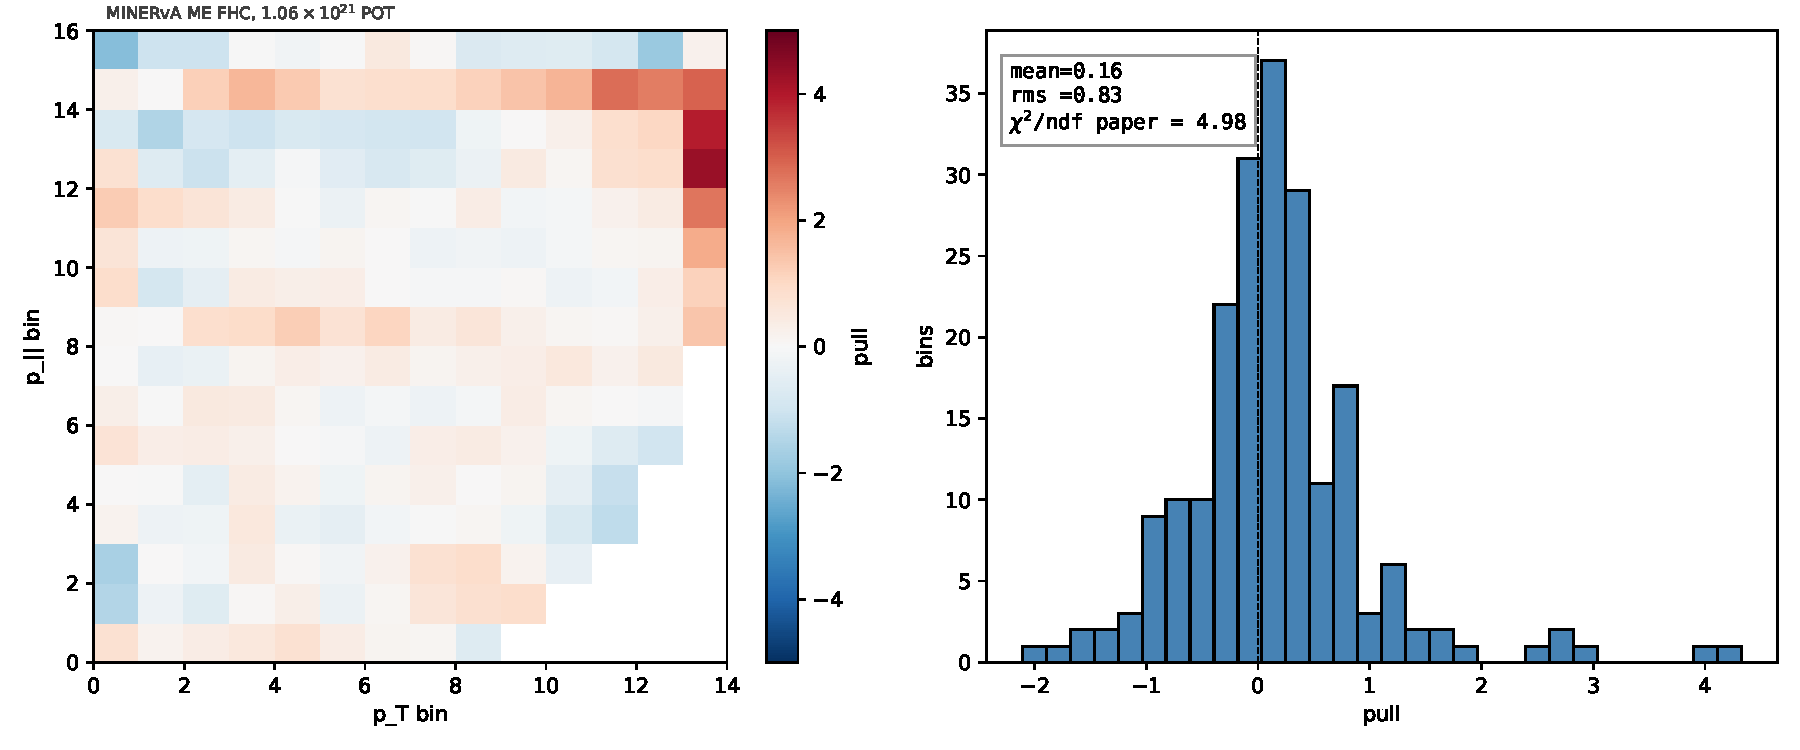
\includegraphics[width=0.7\textwidth]{eavail_marginal_vs_paper_pull_full}
  \caption{Standardized per-bin differences of the $\Eavail$-marginal, scaled by
  published uncertainties, on the $14\times16$ grid and in distribution.
  Shared data and unavailable cross-covariance make these descriptive;
  they are not formal independent-result pulls.}
  \label{fig:eavail-marg}
\end{figure}

\subsection{Closure: the one injected $\Eavail$ deformation is recovered}
\label{sec:3d-closure}
A reweight closure isolates whether the $\SI{4.4}{\percent}$ scatter reflects
method bias or real information. The 3D unfold recovers a known
$+\SI{30}{\percent}$ Gaussian bump injected into pseudo-data in \emph{truth}
$\Eavail$ (center \SI{0.3}{GeV}, width \SI{0.15}{GeV}).
The recovered step-2 mean weight is $1.048$ against the injected $1.0485$.
Residuals against reweighted truth on the $\Eavail$-marginal have median
$0.9999$ and standard deviation \textbf{\num{0.0006}}
(\SI{0.06}{\percent}); the per-3D-bin residual standard deviation is
\SI{3.2}{\percent} from MC statistics in sparse high-recoil corners.
Marginal scatter is $\sim70\times$ tighter than the
$\SI{4.4}{\percent}$ data-versus-2D scatter; total normalization matches
to better than \SI{1}{\percent}. In the metric of \S\ref{sec:validation}
($\Eavail$ projection) the residual is \SI{1.84}{\percent} vs \SI{18.1}{\percent}
injected (ratio $0.102$); the 3D test passes.

\emph{What closes, stated exactly.} The deformation recovered is one shape: a
$+\SI{30}{\percent}$ Gaussian in truth $\Eavail$ at
center~\SI{0.3}{GeV}, width~\SI{0.15}{GeV}, injected into the pseudo-data and
unfolded \emph{with the same detector response the unfold was given}. On that
test the method does not manufacture or destroy the feature, which is what
makes the data-versus-2D scatter readable as
data\,$\leftrightarrow$\,MC structure resolved by the available-energy
dimension rather than as an artifact of this particular injection. It does
\emph{not} exclude estimator bias for other deformations or test response
mismatch, and the hidden-variable closure exceeds its threshold at the largest
amplitude (\S\ref{sec:validation}, App.~\ref{app:response-mismatch}).

\subsection{Classifier-family cross-check (GBDT vs.\ NN)}
\label{sec:3d-classifier}
Our gradient-boosted decision trees differ from the neural-network classifiers
used in published OmniFold analyses~\cite{Andreassen:2019cjw,unbinnedguide}.
GBDT output must be a calibrated posterior for $w=p/(1-p)$ to hold.
The step-1 reco classifier (data vs.\ MC reco) has a near-diagonal reliability
curve, Brier \(\approx0.25\) at AUC \(\approx0.537\).
Data and reco MC are nearly indistinguishable, so the reweight is a modest correction.
A full scalar Keras-MLP cross-check with the same weighted 3D inputs and
five-iteration OmniFold loop gives total ratio $1.0078$ versus GBDT and median projection
differences of \SIrange{0.7}{1.4}{\percent} (Fig.~\ref{fig:calibration}).
Agreement in the populated bulk establishes that the scalar result is not
specific to the production classifier family. Section~\ref{sec:pet-shape}
reports the diagnostic cross-check using low-level recoil point clouds in
place of engineered scalars.

\begin{figure}[H]
  \centering
  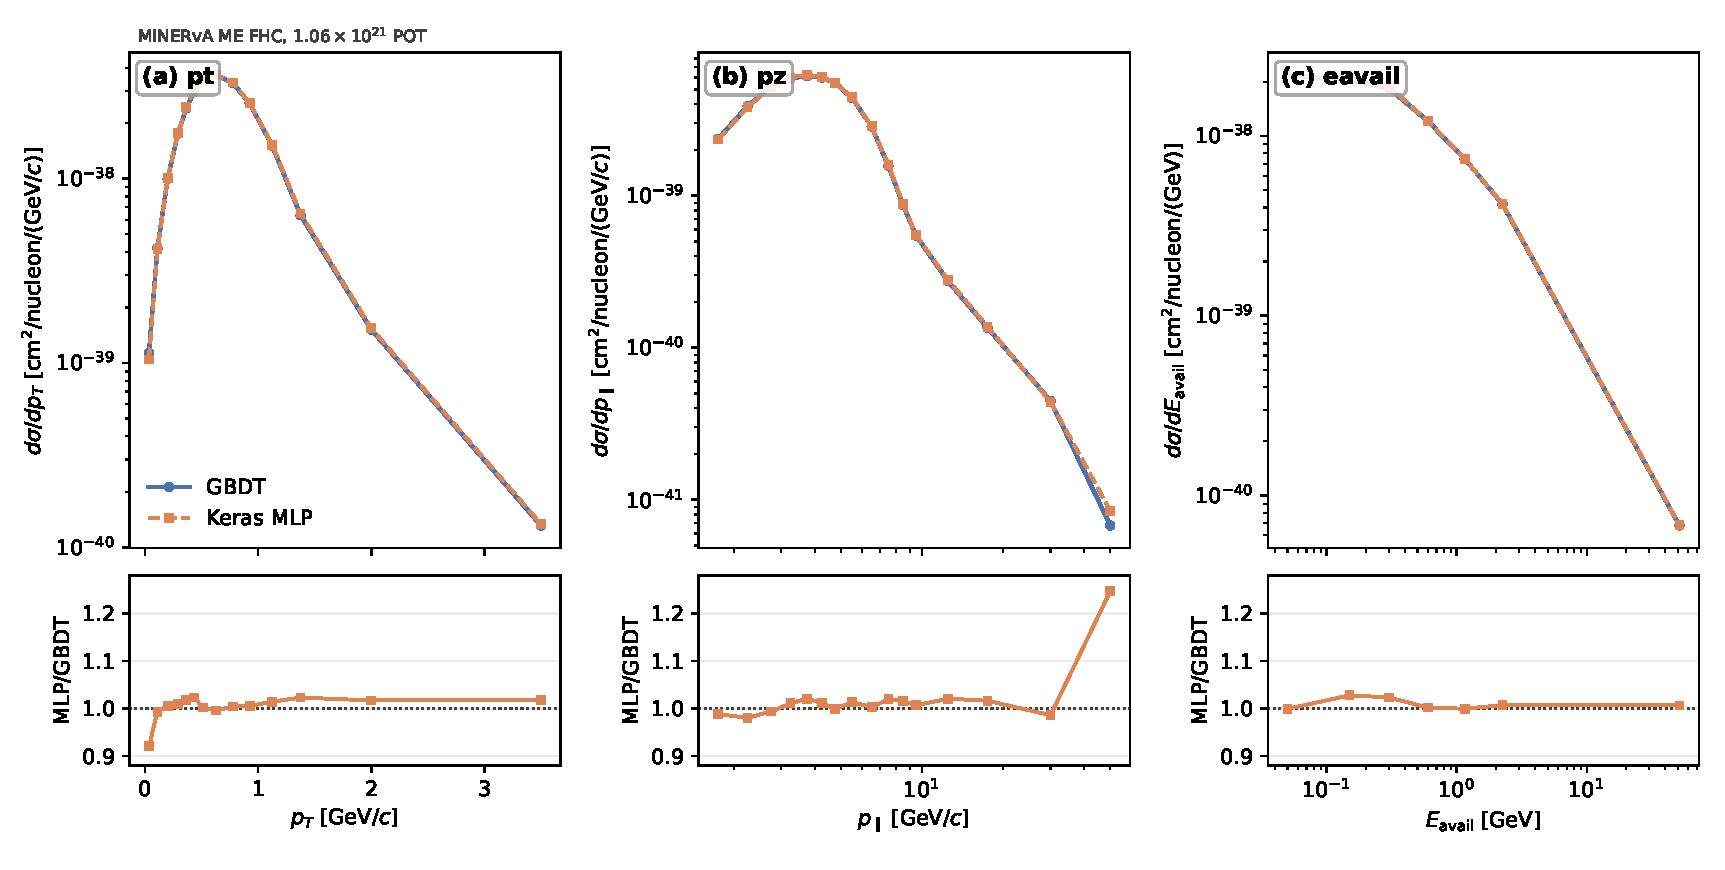
\includegraphics[width=0.95\textwidth]{nn_vs_gbdt_full}
  \caption{Five-iteration scalar OmniFold cross-check with identical weighted
  3D inputs and extraction, changing only the classifier family. Top:
  absolutely normalized GBDT and Keras-MLP projections; bottom: binwise ratio.
  The MLP/GBDT total-cross-section ratio is $1.0078$; median
  absolute projection differences are \SI{1.20}{\percent} in $\pT$,
  \SI{1.36}{\percent} in $\pPar$, and \SI{0.66}{\percent} in $\Eavail$.
  Larger excursions occur only in sparsely populated outermost
  $\pT$ and $\pPar$ bins.}
  \label{fig:calibration}
\end{figure}

\subsection{Generator comparison in 3D}
\label{sec:3d-models}
The ancillary provides only binned 2D model histograms. Quantitative 3D
comparisons or arbitrary projections require generating truth-level
events, histogrammed as $d^{3}\sigma$ in the same fiducial phase space with the
same truth $\Eavail$ definition. The unfolded result is at truth level, so comparisons need no detector
simulation. We generated and processed GENIE, NuWro
and GiBUU samples, and extracted MINERvA Tune~v1 from analysis MC truth with
its full tune weight. No spectra were digitized or externally supplied.
\begin{itemize}
  \item \textbf{GENIE 2.12.10 central value}, generated with \texttt{gevgen}
        on a CH target with the MINERvA ME~FHC flux, using the
        DefaultPlusValenciaMEC cross-section splines~\cite{Andreopoulos:2009rq}
        but gevgen's default event-generator list, which excludes MEC, so
        the sample has no 2p2h events (\S\ref{sec:3d-2p2h}); it has no MINERvA reweights;
        events are reweighted to the analysis flux as described below.
  \item \textbf{MINERvA Tune v1}, the analysis tune (base GENIE $+$ RPA,
        low-recoil 2p2h, and non-resonant-pion reweights), extracted directly
        from event-loop MC truth, which
        % (the \texttt{w\_truth} weights)
        reproduces the shipped ancillary curve to \SI{0.01}{\percent} in
        normalization.
  \item \textbf{NuWro 21.09}~\cite{Golan:2012wx}, an independent generator
        on C with the same flux (after reweighting below) and phase space.
  \item \textbf{GiBUU 2019}~\cite{Buss:2011mx}, a transport-theory generator
        on C, built and run \emph{natively} on the compute system without a
        container, with the same flux and phase space.
\end{itemize}
NEUT~\cite{Hayato:2009zz} is not included.
Each prediction is normalized by its own flux-averaged total CC cross section
per nucleon.

\paragraph{Flux repair of the GENIE and NuWro predictions.}
% (2026-09-27)
GENIE (CV and $+$Valencia~2p2h) and NuWro were initially generated from a flux
without PPFX weights, capped at \SI{50}{GeV}. Variable-width bins stored flux
\emph{densities} but were sampled and normalized by \emph{content}.
Under-weighting every wide high-energy bin suppressed high-$\pPar$ predictions
and integrated rates (App.~\ref{app:provenance}, \texttt{flux-repair}).
% KNOWN_ISSUES.md row 83
GENIE and NuWro predictions throughout \S\S\ref{sec:3d}--\ref{sec:eavailw} are
repaired by exact per-event reweighting to the analysis PPFX central-value flux
on 0--\SI{100}{GeV}, with correctly sampled 50--\SI{100}{GeV} supplements.
The FSI-dial studies, departure ratio of \S\ref{sec:val-negweight} and
NuWro-shaped prior of \S\ref{sec:fps} retain unrepaired samples, as stated there.
GiBUU reads its own flux and receives an energy-dependent per-event reweight
to the same convention, changing its integrated cross section by a factor
$0.9966$. Its sample still stops at $E_\nu\approx\SI{20}{GeV}$, so it is empty
above $\pPar\approx\SI{20}{GeV/c}$.
% KNOWN_ISSUES.md row 82
Comparisons here and in \S\ref{sec:eavailw-band} were rebuilt with unchanged
figure producers on repaired inputs (App.~\ref{app:history}).
% rebuilt on 2026-09-27; ledger rows VL156--VL160 (App. E flux-repair), which supersede VL35--VL38 (App. H, pre-repair values)
The analysis simulation, MINERvA Tune~v1, is unaffected.

Figure~\ref{fig:3dmodels} compares central values only. Totals over the full
measurement phase space follow
GiBUU ($\SI{2.22e-38}{}$) $<$ NuWro ($\SI{2.66e-38}{}$) $<$ Tune v1
($\SI{2.71e-38}{}$) $<$ GENIE CV ($\SI{2.76e-38}{}$) $<$ data
($\SI{3.08e-38}{cm^2/nucleon}$). All four under-predict the rate by
\SIrange{10}{28}{\percent} of the data. Integrating the reported $\Eavail$ range
with the catch bin dropped gives the same order. All closely track the
$(\pT,\pPar)$ shape. The $\Eavail$ axis discriminates among them;
NuWro and Tune v1 \emph{suppress} the lowest-$\Eavail$ (quasielastic) bin
below bare GENIE through RPA and nuclear effects, while GiBUU does not.
Data lie \emph{above} all four across the quasielastic--$\Delta$ dip,
$0.1\le\Eavail<\SI{0.4}{GeV}$ (in the lowest bin GiBUU reaches the data).
The $\Eavail$ axis exposes this excess, invisible in 2D.

\begin{figure}[H]
  \centering
  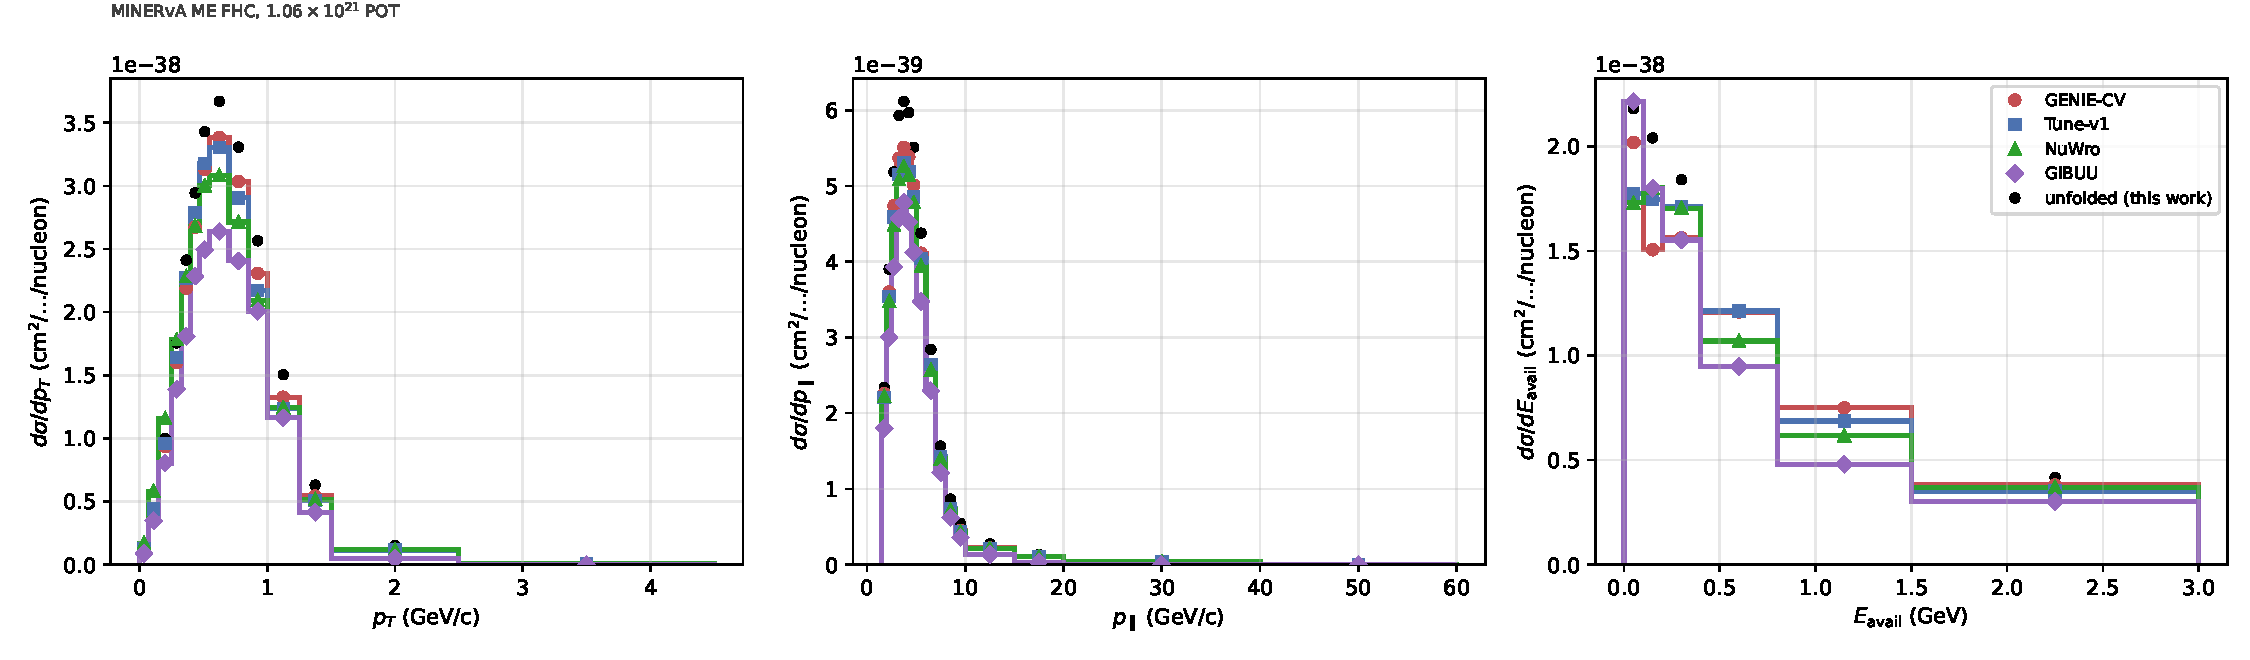
\includegraphics[width=0.99\textwidth]{generators_vs_unfolded_band_central}
  \caption{1D projections of the unfolded 3D central cross section (black)
  versus truth-level predictions from GENIE 2.12 CV, MINERvA Tune v1, NuWro 21.09, and
  GiBUU 2019 (GENIE and NuWro: the flux-repaired predictions,
  \S\ref{sec:3d-models}). Models track the $\pT$ and $\pPar$ shapes but differ
  on $\Eavail$; all under-predict the quasielastic--$\Delta$
  dip ($0.1\le\Eavail<\SI{0.4}{GeV}$). The wide
  $\Eavail$ catch bin is omitted from the axis.
  Data have no error bars because the quotable
  3D covariance is not yet adopted (App.~\ref{app:history}).}
  \label{fig:3dmodels}
\end{figure}

For the integrated $\Eavail$ rate without the catch bin, GENIE CV, Tune~v1,
NuWro and GiBUU central values lie respectively
$\SI{7.2}{\percent}$, $\SI{9.5}{\percent}$, $\SI{12.8}{\percent}$ and
$\SI{22.2}{\percent}$ below the data.
% (flux-repaired predictions; ledger row \texttt{VL159})
No 3D covariance, generator $\chi^{2}$, $p$-value or significance is quoted:
the quotable 3D covariance is the exact projection of the adopted 5D covariance,
and that projection is constructed but not adopted (App.~\ref{app:history}).

\subsection{The low-available-energy excess recovers the known low-recoil 2p2h deficit}
\label{sec:3d-2p2h}
The low-$\Eavail$ excess is the most physically interesting feature the third
axis exposes, and the 3D framework lets us test candidate explanations by
generating the relevant physics as well as reweighting. MINERvA first isolated the rate enhancement between quasielastic
and $\Delta$ peaks, with multi-nucleon final states, in a
low-three-momentum-transfer subsample~\cite{MINERvA:2016lowrecoil}.
The empirical tune was built to absorb it; our muon-kinematics
$\times\,\Eavail$ measurement re-exposes that established low-recoil feature.

\paragraph{The tested pion-FSI variations do not account for it.}
A \texttt{grwght1p} reweight of 2M central-value GENIE events gives sub-percent
changes in $d\sigma/d\Eavail$ for both tested pion-FSI dials.
\texttt{FrInel\_pi} shifts the spectrum by
$\le\SI{0.74}{\percent}$ (peak in $0.10$--$\SI{0.20}{GeV}$) and \texttt{FrAbs\_pi}
by $\le\SI{0.82}{\percent}$ (peak in the lowest bin). Both use the pre-repair
GENIE sample (\S\ref{sec:3d-models}) as same-sample ratios, where the flux
defect cancels to first order; neither was recomputed. The integrated rate
% flux repair: KNOWN_ISSUES.md row 83
moves only $\pm\SI{0.02}{}$--$\SI{0.03}{\percent}$ at $\pm1\sigma$.
\footnote{\texttt{FrInel\_pi} is commented out of the standard MAT-MINERvA systematics
registry. In 2026 the collaboration confirmed this remains current practice
and that the reason is a degeneracy (overlapping pion-FSI dials require
dropping one), rather than a defect specific to that knob.}
A less-than-\SI{1}{\percent} knob cannot bridge an excess of
\SIrange{8}{36}{\percent} per bin over the GENIE central value below
$\Eavail=\SI{0.4}{GeV}$. The tested variations do not account for the excess,
a conclusion limited to these dials and their range. Other transport models
or proton-FSI effects are not excluded. Recent MINERvA quasielastic-like
measurements point toward overestimated proton and charged-pion FSI in their model
comparisons~\cite{MINERvA:2026qeleme}. Their different signal definition prevents
directly identifying that effect with our inclusive discrepancy.

\paragraph{The shape and size match 2p2h.} The base GENIE central value uses
the default event-generator list and contains \emph{no}
meson-exchange-current (2p2h/MEC) events
($\texttt{mec}=0$ for all $1.48\times10^{6}$ CC events of the generated
sample, whose unweighted modes, before the flux reweight of
\S\ref{sec:3d-models}, are QE
\SI{11}{\percent}, RES \SI{22}{\percent}, DIS \SI{66}{\percent}, COH
\SI{0.9}{\percent}; the 50--\SI{100}{GeV} supplement is MEC-free as well).
2p2h must therefore be \emph{added}; reweighting cannot supply it.
The mode decomposition of central-value $d\sigma/d\Eavail$ (per-bin mode
count-fractions $\times$ bin value), overlaid with data, locates the largest
positive gaps in the quasielastic--$\Delta$ dip,
$[0.10,0.20)$ and $[0.20,0.40)$, while central values are much closer in the
QE-dominated $[0,0.10)$ and $[0.40,1.50)$ regions.
At central value, \SI{70}{\percent} of the positive deficit lies at
$\Eavail\le\SI{0.4}{GeV}$, exactly where 2p2h lives. Closing the integrated deficit
requires 2p2h at $\approx\SI{45}{\percent}$ of the QE rate
(\SIrange{68}{71}{\percent} in the two dip bins), the standard
empirical/Valencia-MEC magnitude, compared with sub-percent FSI shifts
(Fig.~\ref{fig:modedecomp}).

\paragraph{Enabling Valencia 2p2h improves the description.} We regenerated the GENIE central
value with empirical 2p2h enabled (\texttt{--event-generator-list
Default+CCMEC}, 2M events). Because the Nieves--Simo--Vacas MEC channel, though
present in the splines, is absent from the \texttt{gspl2root} total-CC graph, we
normalize by the non-MEC CC count, anchoring QE$+$RES$+$DIS$+$COH to the known total and
adding MEC through $1/(1-f_{\mathrm{MEC}})$ with
$f_{\mathrm{MEC}}=\SI{2.87}{\percent}$.
2p2h falls in the dip and brings all three low-$\Eavail$ bins toward data
(Fig.~\ref{fig:mec}), filling
\SI{52}{\percent} of the data$-$CV gap at $\Eavail\le\SI{0.4}{GeV}$ and \SI{63}{\percent} of the
integrated deficit (CV $-\SI{7.2}{\percent}\to-\SI{2.6}{\percent}$;
App.~\ref{app:history}). The prediction
% ledger row \texttt{VL160}
still falls short in the dip, especially $[0.10,0.20)$, but its integral over
the reported $\Eavail$ range is closer to data than
Tune~v1 ($-\SI{2.6}{\percent}$ against $-\SI{9.5}{\percent}$). Tune v1
layers MINERvA's empirical low-recoil 2p2h \emph{enhancement} and RPA on top of
the stock Valencia MEC --- i.e.\ stock Valencia 2p2h is real but under-strength
for MINERvA low recoil, which is precisely the known MINERvA-tune story and is
consistent with NuWro and GiBUU (native, un-enhanced 2p2h) sitting low in the
dip as well.

2p2h leaves the high-$\Eavail$ $[1.50,3.00)$ bin unchanged. There, data
exceed the GENIE CV by about \SI{9}{\percent} (data/CV $1.09$;
App.~\ref{app:history}) and exceed Tune~v1 as well; the high-$\Eavail$
excess over Tune~v1 is localized on the $(\Eavail,W)$ plane in
\S\ref{sec:eavailw}.

The improvement supports the tested multinucleon contribution's relevance
without uniquely identifying a nuclear mechanism. For example, recent NEUT studies include
two-body currents contributing to one-particle--one-hole final states and examine their
interplay with axial form factors
\cite{FrancoMunoz:2026currents}. A two-body current is not synonymous with the
generator's 2p2h event category. Visible-energy comparisons can depend on the
primary interaction and subsequent hadronic transport.

Ascencio \emph{et al.}~\cite{MINERvA:2022incl} report the same deficit in
MINERvA's dedicated low-recoil inclusive $d^{2}\sigma/(dq_{3}\,d\Eavail)$
measurement for $q_{3}<\SI{1.2}{GeV}$ at the same
$\langle E_\nu\rangle\sim\SI{6}{GeV}$, finding GENIE and NuWro underpredicting
their low-$\Eavail$ data without enhanced 2p2h. Our muon-kinematics extension integrates all $q_3$
instead of fixing $q_3$, limiting comparison to $\Eavail$ \emph{shape} and
direction, without absolute normalization. The consistency confirms recovery
of the established MINERvA low-recoil/2p2h feature as a by-product of the
OmniFold 3D muon-kinematics unfolding. Bin-identical central values follow in
\S\ref{sec:4d}.

\begin{figure}[H]
  \centering
  \begin{minipage}{0.49\textwidth}
    \centering
    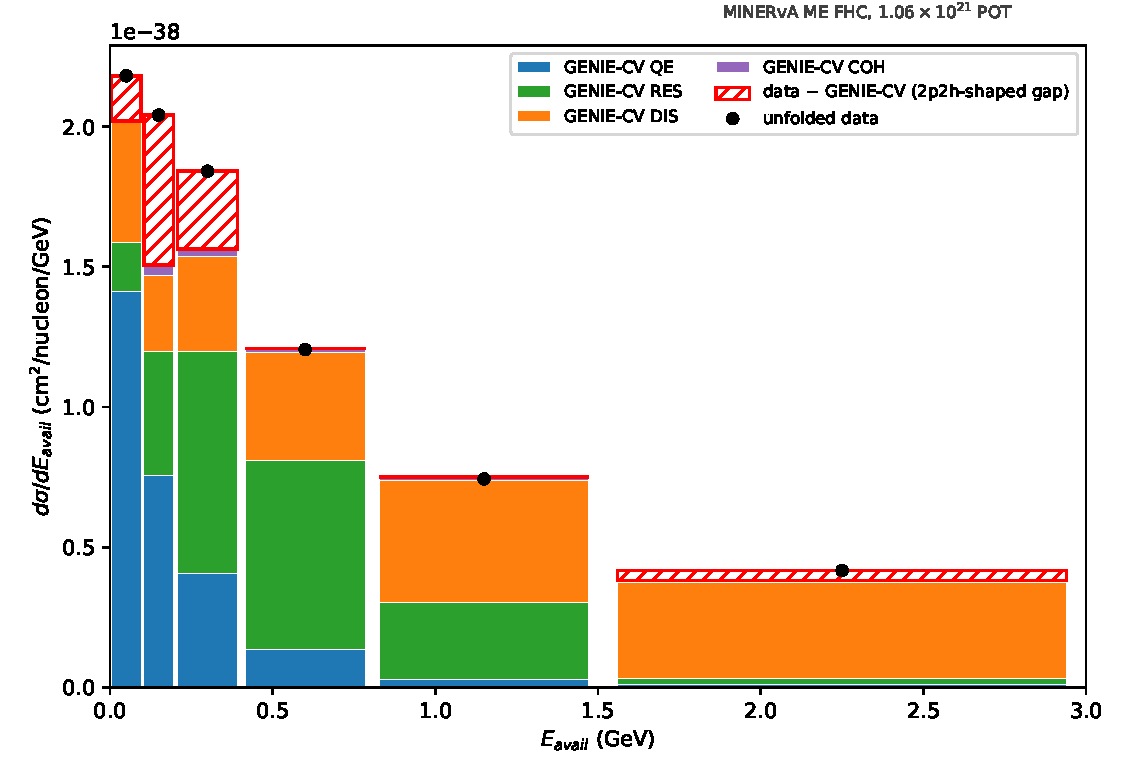
\includegraphics[width=\textwidth]{mode_decomp_eavail_central}
    \caption{Central-value $d\sigma/d\Eavail$ by interaction mode, overlaid
    with unfolded data. The excess lies in the quasielastic--$\Delta$ dip
    ($\Eavail\le\SI{0.4}{GeV}$), matching a missing 2p2h component's shape and
    size. Data carry no error bars because the quotable 3D covariance is not
    yet adopted (App.~\ref{app:history}).}
    \label{fig:modedecomp}
  \end{minipage}\hfill
  \begin{minipage}{0.49\textwidth}
    \centering
    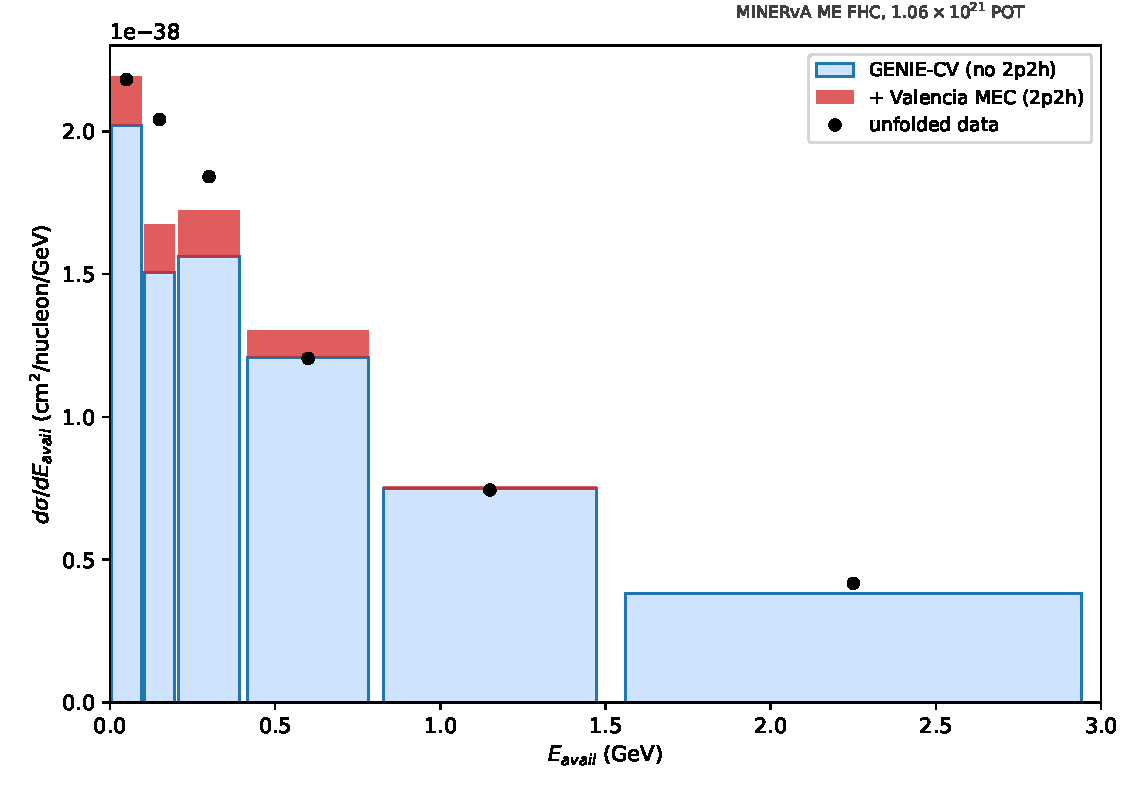
\includegraphics[width=\textwidth]{compare_mec_eavail_central}
    \caption{GENIE regenerated with empirical Valencia 2p2h (red, stacked on
    no-2p2h CV; both flux-repaired) fills about half the low-$\Eavail$
    data$-$CV gap (\SI{52}{\percent}). The remainder occupies the region the
    MINERvA tune's empirical enhancement is built to absorb. Data carry no
    error bars because the quotable 3D covariance is not yet adopted
    (App.~\ref{app:history}).}
    \label{fig:mec}
  \end{minipage}
\end{figure}

\subsection{Fourth axis: three-momentum transfer $q_{3}$}
\label{sec:4d}
The fourth axis adds one feature (\S\ref{sec:3d}), three-momentum transfer
$q_{3}=|\vec{q}\,|$, chosen because its $(\Eavail,q_{3})$ plane separates
quasielastic, 2p2h and resonance processes and permits bin-compatible comparison to MINERvA's
dedicated low-recoil $d^{2}\sigma/dq_{3}\,d\Eavail$ measurement
(Ascencio \emph{et al.}~\cite{MINERvA:2022incl}). Truth $q_{3}$ comes from
the generator (\texttt{CVUniverse::Getq3True()}); reco $q_{3}$ uses muon
$Q^{2}$ and calorimetric recoil (\texttt{CVUniverse::RecoQ3()}). Both accessors
run over all twelve playlists, as for $\Eavail$. Lateral systematic shifts
change $q_{3}$ but leave $\Eavail$ invariant, requiring per-universe
shifted-$q_{3}$ dumps instead of central-value reuse.
The feature stack is $(\pT,\pPar,\Eavail,q_{3})$, with deliberately coarse
$q_{3}$ binning $[0,0.2,0.4,0.6,0.8,1.2,2.0,100]\,\si{GeV}$
(seven bins including a final catch bin), giving
$14\times16\times7\times7=10\,976$ four-dimensional bins (4830 populated).

\paragraph{Marginal anchor (4D$\to$3D).} The $q_{3}$ marginalization reproduces
the 3D $\Eavail$ spectrum and low-recoil excess (Fig.~\ref{fig:q3excess}, right).
The $\Eavail$-marginal data/Tune~v1 ratio is
$1.21$ in the lowest bin, dips to $1.01$ across the quasielastic--$\Delta$
region, and rises to $1.16$--$1.23$ in the high-$\Eavail$ DIS tail
(integrated data/Tune~v1 $=1.13$). These ratios compare to Tune~v1;
\S\ref{sec:3d-2p2h} uses untuned GENIE. Recovery as a by-product
of the higher-dimensional unfold provides the 4D$\to$3D analog of the
3D$\to$2D Jacobian anchor (\S\ref{sec:3d-anchor}).

\paragraph{What $q_{3}$ adds.} The resolved $(\Eavail,q_{3})$ plane
(Fig.~\ref{fig:q3excess}, left) reveals structure beneath the mild
$q_{3}$-marginal discrepancy integrated over $\Eavail$
($1.03$--$1.19$, center). At fixed $\Eavail$
in the quasielastic--$\Delta$ dip, data/Tune~v1 \emph{rises} with $q_{3}$.
The central value over-predicts low-$q_{3}$, moderate-$\Eavail$ cells
(ratio down to $0.66$); data excess concentrates at low $\Eavail$ (all $q_{3}$)
and toward high $q_{3}$. The muon-only or fixed-$q_{3}$ projections considered
here do not resolve this correlation, a natural input to the bin-compatible
Ascencio comparison. The map uses central values and the MINERvA Tune~v1
prior, distinct from the untuned GENIE sample of \S\ref{sec:3d-2p2h}
(App.~\ref{app:provenance}, \texttt{q3-excess}). No per-cell significances
are reported without a corrected 4D covariance (below).
% comparator weights: \texttt{w\_truth}; script \texttt{nd-unfolding/q3\_excess\_projection.py}

\paragraph{Why no 4D uncertainty is reported.} Corrected 4D covariance would use actual
minus/plus endpoints, MAT mean-centered $1/N$ blocks, one fixed estimator seed,
mean-centered joint throws with a separately reported mean shift, and no scalar
jitter subtraction. Because dump-all lateral branches are CV-support-limited,
selection-complete active-universe event loops must bound migration effects.
No 4D uncertainty magnitude or unified/block ratio is reported.

\paragraph{Bin-identical comparison to the published low-recoil measurement.}
Supplemental data from Ref.~\cite{MINERvA:2022incl} (44-cell
$d^{2}\sigma/(d\Eavail\,dq_{3})$ with its full covariance, distributed inside
the public arXiv source package) permit a direct quantitative cross-check.
Merging both measurements onto their maximal common grid --- edges present in
\emph{both} binnings --- and restricting our
$(\pT,\pPar)$ marginalization to $\pPar<\SI{20}{GeV/c}$ to mirror the Ascencio
muon gate ($\theta_\mu<20^{\circ}$, $1.5<p_\mu<\SI{20}{GeV}$) gives two super-cells,
$\Eavail<\SI{0.4}{GeV}$ in $q_{3}\in[0.4,0.6)$ and $[0.6,1.2)\,\si{GeV}$: the
low-recoil 2p2h region. Our central result lies
\SI{9.2}{\percent} and \SI{6.3}{\percent} above Ascencio. No pulls or
full-covariance $\chi^{2}$ are reported (no corrected 4D covariance, above;
Fig.~\ref{fig:ascencio}). Both share MINERvA flux/detector systematics,
treated here as independent. The $p_\mu$-vs-$\pPar$ gate differs by
$\lesssim\SI{6}{\percent}$ kinematic smearing at the \SI{20}{GeV} boundary.
A finer 44-cell comparison remains future work; it requires re-unfolding on
Ascencio edges (trivial for the unbinned method) \emph{and} a systematic
sweep on that binning.

\begin{figure}[H]
  \centering
  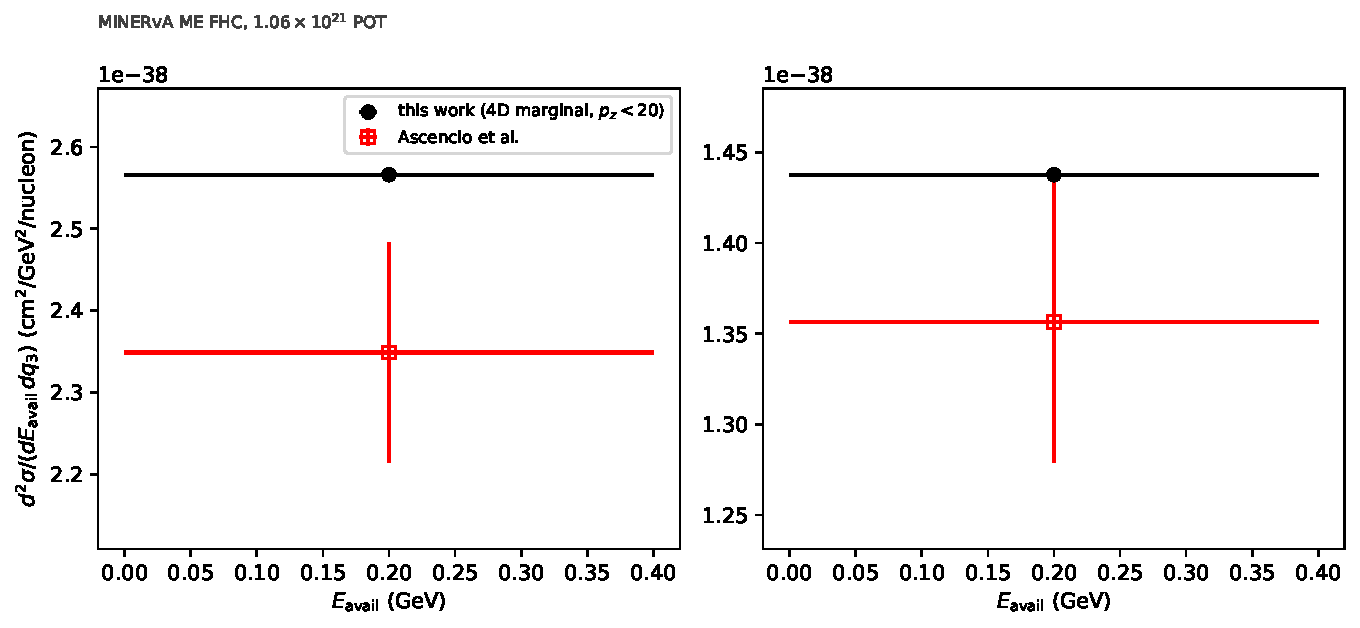
\includegraphics[width=0.85\textwidth]{ascencio_fullcov_compare_central}
  \caption{Bin-identical comparison to Ascencio
  \emph{et al.}~\cite{MINERvA:2022incl} on the maximal common
  $(\Eavail,q_{3})$ grid, used only for central-value comparison. Our points
  have no uncertainty or $\chi^{2}$ drawn because the
  quotable 4D covariance is not yet adopted (App.~\ref{app:history}); the
  published points carry the published covariance.}
  \label{fig:ascencio}
\end{figure}

\begin{figure}[H]
  \centering
  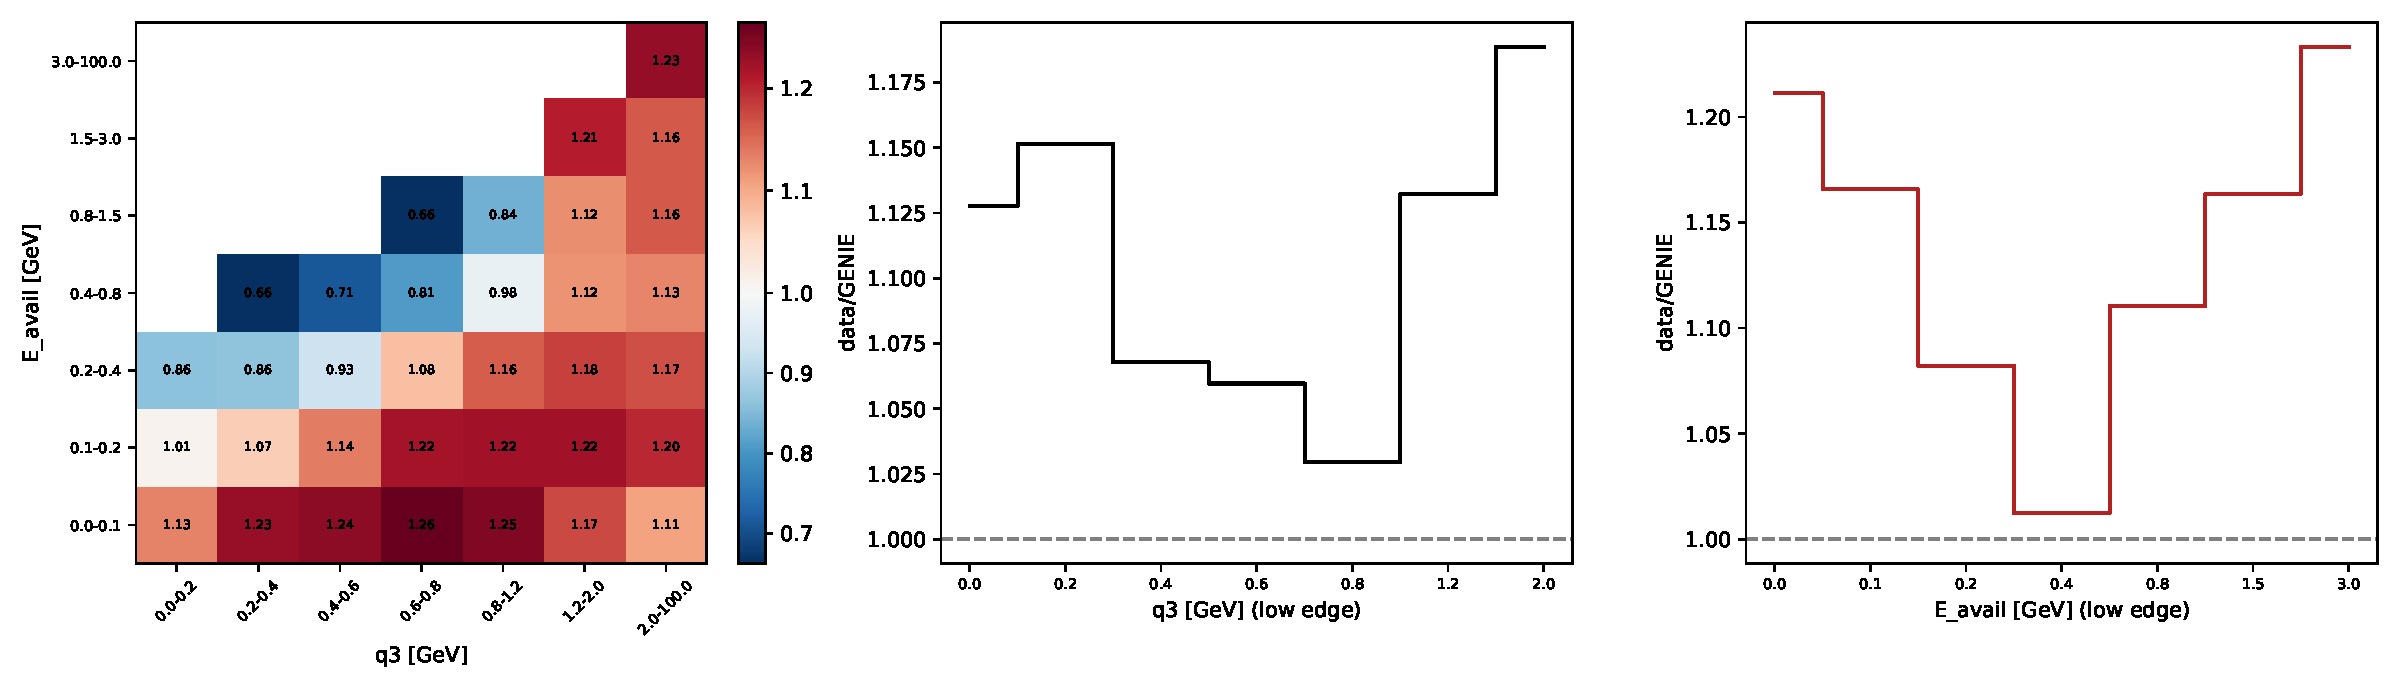
\includegraphics[width=0.99\textwidth]{q3_excess_projection}
  \caption{4D data/Tune~v1 ratio (``data/GENIE'' in the figure) projected onto
  $(\Eavail,q_{3})$ (left; blank cells are kinematically empty), with
  $q_{3}$ (center) and $\Eavail$ (right) marginals. The $\Eavail$ marginal
  reproduces the 3D low-recoil excess. The joint plane shows genuine $q_{3}$
  structure in the data\,$-$\,MC discrepancy (ratio rising with $q_{3}$
  across the quasielastic--$\Delta$ dip).}
  % Comparator: the MINERvA Tune~v1 prior (\texttt{w\_truth}).
  \label{fig:q3excess}
\end{figure}

\section{Fifth axis: the $(\Eavail,W)$ deep-inelastic-tail study}
\label{sec:eavailw}

Valencia 2p2h fills about half the low-recoil gap
(\S\ref{sec:3d-2p2h}), leaving a separate high-$\Eavail$ excess over the
MINERvA Tune~v1 prior. Here 2p2h contributes nothing and the sub-percent
pion-FSI dials cannot reach the excess (covariance qualifications in
\S\ref{sec:eavailw-adopted}). External-generator comparisons depend on the
model. GiBUU is low throughout the $\Eavail$ tail ($W$-integrated data/generator $1.59$
at $\Eavail\in[0.8,1.5)$ and $1.37$ at $[1.5,3.0)$;
\S\ref{sec:eavailw-band} discusses its $E_\nu\approx\SI{20}{GeV}$ limit).
GENIE CV matches $[0.8,1.5)$ and is low in $[1.5,3.0)$ (data/CV $1.09$)
(\S\ref{sec:3d-2p2h}). Adding hadronic invariant mass $W$ as the fifth
OmniFold axis tests the deep-inelastic hypothesis directly.
Validation in \S\ref{sec:val-fiveaxis} includes a model-dependence study;
it establishes no bias--variance tradeoff or new total uncertainty for this projection.

\subsection{$W$ as a fifth axis}
\label{sec:eavailw-axis}

Truth $W$ is the experimenter's invariant mass
$W=\sqrt{M^{2}+2M(E_\nu-E_\mu)-Q^{2}}$, with struck-nucleon mass $M$
(\texttt{CVUniverse::GetTrueExperimentersW()}). Reco $W$ uses the reco
$q_{3}$ estimator's calorimetric transfer $q_{0}$ and muon-kinematic $Q^{2}$,
with the average nucleon mass (\texttt{CVUniverse::RecoW()}). Like $q_{3}$ --- and unlike $\Eavail$ --- $W$
is not invariant under the lateral systematic shifts, so the event loop dumps
shifted-$W$ lateral universes per universe, mirroring the $q_{3}$ treatment
(\S\ref{sec:4d}); the dump also carries truth hadronic diagnostics (proton and
pion multiplicities, leading-hadron angle). The $W$ edges
$[0,1.1,1.4,1.8,2.2,3.0,100]\,\si{GeV}$ bracket the quasielastic peak,
$\Delta$, transition region and DIS tail. The five-axis unfold
$(\pT,\pPar,\Eavail,q_{3},W)$ passes its predecessors' marginalization
anchors. Integrating over $W$ recovers the frozen 4D normalization to
\SI{\eavailMargin}{\percent} (5D/4D total $=1.0011$), with per-axis median
differences of \SIrange{0.3}{1.5}{\percent}; $d\sigma/dW$ is finite and
non-negative in all six bins.

\subsection{Where the excess lives in the $(\Eavail,W)$ plane}
\label{sec:eavailw-map}

Projecting the unfolded five-axis result onto $(\Eavail,W)$ and subtracting
the MINERvA Tune~v1 prediction localizes the excess
(Fig.~\ref{fig:eavailWexcess}): it is \emph{predominantly deep-inelastic}.
The prediction is the OmniFold prior, the simulation's truth weighted by its
full tune weight.
% full tune weight: \texttt{w\_truth}
Untuned GENIE~CV in \S\ref{sec:eavailw-band} is a separate prediction.
The two highest-$\Eavail$ bands carry \SI{57}{\percent} of the positive excess.
High-$\Eavail$ ($\ge\SI{0.8}{GeV}$) contains \SI{67}{\percent} of all positive
excess, with \SI{83}{\percent} of that at $W\ge\SI{1.8}{GeV}$. The largest
cell, the deep-DIS corner ($\Eavail>\SI{3}{GeV}$, $W>\SI{3}{GeV}$), holds
\SI{22}{\percent}. A secondary low-$W$ QE-like excess lies below \SI{1.1}{GeV},
with a small deficit in the $\Delta$ region ($W\simeq1.4$--$\SI{1.8}{GeV}$).
These are central-value statements under the nominal detector response.
Estimator-seed shifts are a small fraction of the projected uncertainties
(\S\ref{sec:eavailw-adopted}, item~4), but seed sensitivity of the shares,
which are ratios of central-value differences, has not been measured separately.
The response-mismatch closure in
Appendix~\ref{app:response-mismatch} is designed to test whether an incorrect
hadronic response can move strength into or out of the low-$W$ component; it
has not yet produced a result.

\begin{figure}[H]
  \centering
  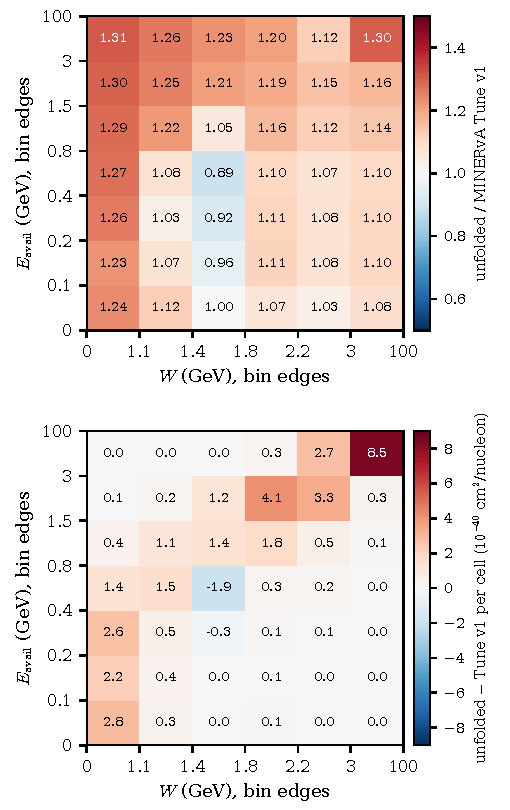
\includegraphics[width=0.55\textwidth]{paper_fig2_joint}

  \caption{Unfolded data and MINERvA Tune~v1 (GENIE~2.12.6 with analysis tune
  weights, the OmniFold prior)
  % tune weights: \texttt{w\_truth}
  in $(\Eavail,W)$. Top gives dimensionless per-cell data/Tune on a
  $0.5$--$1.5$ colour scale; bottom gives per-cell data\,$-$\,Tune in units of
  $10^{-40}\,\si{cm^2/nucleon}$. Equal-size display cells are labelled by
  physical bin edges on the
  $7\times6$ reporting grid, with $\Eavail$ edges
  $[0,0.1,0.2,0.4,0.8,1.5,3.0,100]\,\si{GeV}$ and $W$ edges
  $[0,1.1,1.4,1.8,2.2,3.0,100]\,\si{GeV}$. The final interval on each axis,
  $[3,100]\,\si{GeV}$, is a wide catch bin. The density ratio is area-free; the bottom panel
  instead subtracts \emph{cell-integrated} cross sections,
  $(\mathrm{d}^{2}\sigma/\mathrm{d}\Eavail\,\mathrm{d}W)\times
  \Delta\Eavail\,\Delta W$ in \si{cm^2/nucleon}
  (App.~\ref{app:provenance}, \texttt{eavailw-excess}). The catch-bin cells carry
  their large widths and look correspondingly bigger. Together the panels locate the positive excess
  at high $\Eavail$ and high $W$ (deep-inelastic), with a secondary low-$W$
  QE-like component and a small $\Delta$-region deficit. Quoted percentage shares
  refer to cell-integrated positive excess in the bottom panel.}

  \label{fig:eavailWexcess}
\end{figure}

\subsection{Generator band: the corner against four external generators}
\label{sec:eavailw-band}

All four external generators fall below the data in the
high-$\Eavail\times$high-$W$ corner. Figure~\ref{fig:eavailWband} compares spline-normalized
$(\Eavail,W)$ predictions from GENIE~CV, GENIE$+$Valencia~2p2h/MEC, NuWro
and GiBUU, using the flux-repaired predictions of \S\ref{sec:3d-models}
(App.~\ref{app:provenance}, \texttt{flux-repair}).
% rebuilt on 2026-09-27; KNOWN_ISSUES.md row 83; ledger rows VL156--VL158 supersede VL35--VL38 (App. H, pre-repair values)
Both 3D and $(\Eavail,W)$ comparisons use one five-dimensional histogram per
generator; GENIE~CV totals \SI{2.76e-38}{cm^2/nucleon} in phase space in both.
GENIE$+$MEC uses the 3D normalization convention (App.~\ref{app:history}).
% KNOWN_ISSUES.md row 81
% The superseded provenance comment block (SUPERSEDED 2026-09-27 ... RESOLVED 2026-08-12)
% that stood here was moved verbatim to App. H, "Pre-repair values", beside
% "From \S\ref{sec:eavailw-band}, the generator inputs" (group g3 sidecar appH-additions.tex).
In the corner ($\Eavail\ge\SI{0.8}{GeV}$, $W\ge\SI{1.8}{GeV}$),
data/generator $=1.14$, $1.14$, $1.16$ and $1.61$, respectively; none reaches
the data. For GENIE and NuWro this is close to their whole-plane shortfall
(integrated ratios $1.11$, $1.07$ and $1.15$). Their corner ratios exceed their integrated ratios
by \SIrange{1}{7}{\percent}, compared with \SI{16}{\percent} for GiBUU
(integrated $1.39$; $\sigma=\SI{2.22e-38}{cm^2/nucleon}$ versus data
\SI{3.07e-38}{}). GiBUU's larger contrast comes from its sample's energy limit:
it was generated only up
% KNOWN_ISSUES.md row 82
to $E_\nu\approx\SI{20}{GeV}$ (\S\ref{sec:3d-models}). In GENIE and NuWro,
neutrinos above this energy carry \SIrange{14.3}{14.8}{\percent} of the corner
cross section and \SIrange{6.8}{7.4}{\percent} overall. Removing them raises
these generators' corner-to-integrated contrast to \SIrange{9}{16}{\percent},
bracketing GiBUU's. Supplying GiBUU their share instead gives about $1.37$ in
the corner and $1.29$ integrated. Thus the flux-repaired corner has no distinct
deficit for any of the four generators. GiBUU is lower than the others everywhere, and its
energy limit accounts for the larger corner shortfall.
% Source: VALIDATION_LEDGER VL161 (docs/orchestration/state/note-capgap-20261003/); KNOWN_ISSUES 82.

Valencia 2p2h raises the GENIE$+$MEC integrated prediction while leaving the corner
essentially unchanged ($1.142\to1.139$), since it populates low $W$.
At $W\in[2.2,3.0)\,\si{GeV}$, data/generator $=1.12$, $1.11$, $1.13$ and
$1.34$, again close to the integrated ratios. These are central-value ratios; no compatibility metric is quoted, for the
reason given in \S\ref{sec:eavailw-adopted}, item~1.

The localization in \S\ref{sec:eavailw-map} is relative to MINERvA Tune~v1;
data exceed all four external generators both overall and in the corner.

\begin{figure}[H]
  \centering
  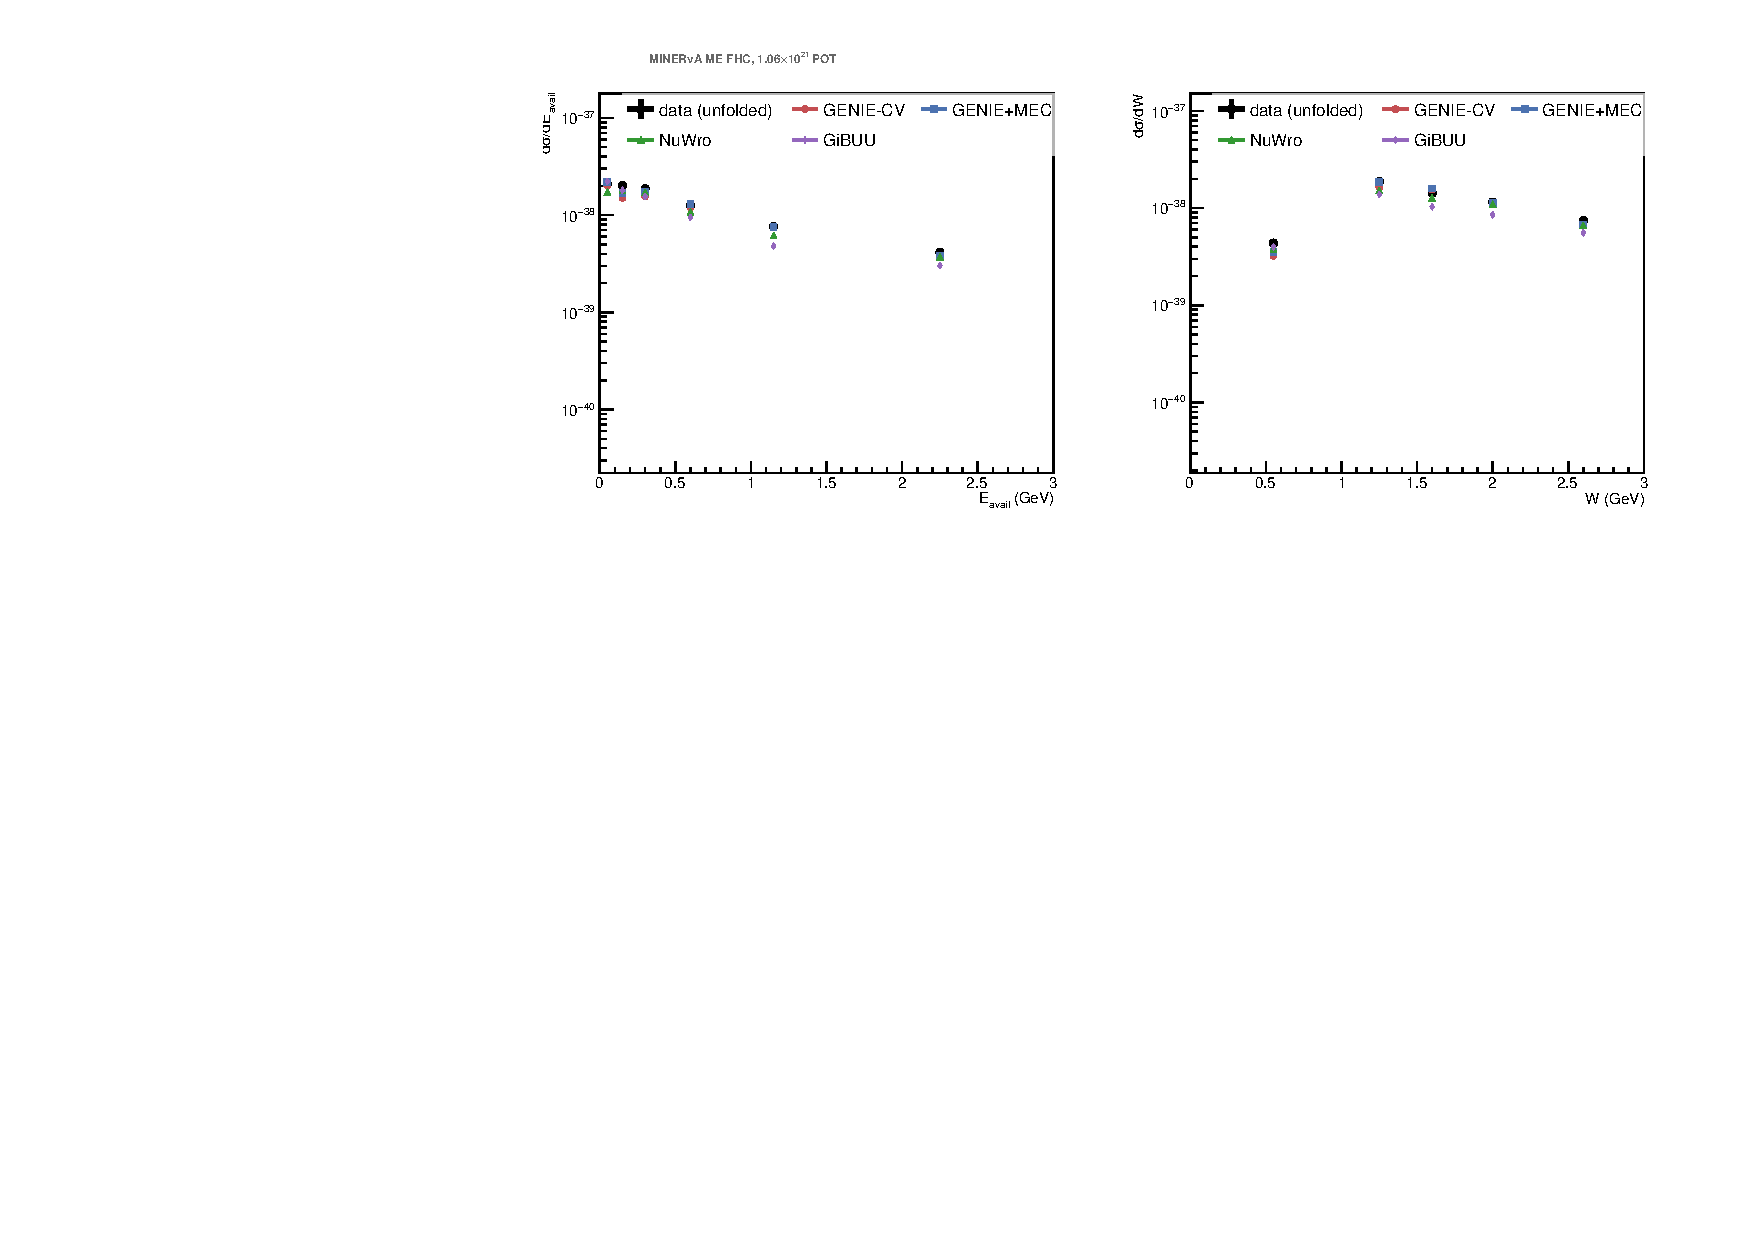
\includegraphics[width=0.99\textwidth]{eavailW_band}
  \caption{Unfolded $(\Eavail,W)$ cross section versus the four-generator
  band (GENIE~CV, GENIE$+$MEC, NuWro, GiBUU; GENIE and NuWro flux-repaired,
  \S\ref{sec:3d-models}). Every generator lies below the data in the high-$W$,
  high-$\Eavail$ DIS corner --- GENIE and NuWro by about their overall
  normalization shortfall, GiBUU by more; adding 2p2h leaves the corner
  unchanged because 2p2h populates low $W$.}
  \label{fig:eavailWband}
\end{figure}

MINERvA shallow-inelastic neutrino and antineutrino measurements also report
shape and normalization disagreements with generators \cite{MINERvA:2025sis}.
They motivate tests across the resonance--DIS transition,
but their selections and reported observables differ from this inclusive
projection. They therefore provide physics context, not an independent
confirmation of the same localized excess. The location identified in the
central-value map is descriptive; a future significance must account for any
selection of the tested region using these data.
The published low-recoil cross-check in $(\Eavail,q_{3})$ (\S\ref{sec:4d})
gives central values \SI{9.2}{\percent} and \SI{6.3}{\percent} above the
published measurement on the maximal common grid, with no reported covariance-based consistency metric.

\subsection{Covariance of the $(\Eavail,W)$ projection}
\label{sec:eavailw-construction}

\paragraph{Status.}
\label{sec:eavailw-adopted}

The adopted five-axis covariance \texttt{z-cv.npz}
(\texttt{sha256}~\zcvDigest\ldots, \num{890500272} bytes, variant \texttt{cv})
has an $(\Eavail,W)$ projection with \texttt{sha256}~\zprojDigest\ldots\ on
\zprojCells\ cells. Its digest-bound exception covers only these bytes.
Metadata still reads $\texttt{scientific\_acceptance}=\text{\texttt{NON-PASSING}}$
and $\texttt{adoptable}=\text{\texttt{false}}$: the specification's null bound
could not be fixed before production (App.~\ref{app:release-audit}).
The earlier direct 42-bin $(\Eavail,W)$ block sum (\S\ref{sec:eavailw-cov})
is superseded and quoted nowhere in this note (App.~\ref{app:history}).

\paragraph{Construction.} The adopted object projects the corrected five-axis
statistical covariance as $M C_{5D}M^{\top}$, without rebuilding it in the
destination bins, and uses corrected systematic endpoints. Selection-complete
active-universe event loops now bound migrations omitted by the
CV-support-limited dump-all sample (\S\ref{sec:uq-higherdim}). On the
$\latBins$ reported cells of $(\pT,\pPar,\Eavail,q_{3},W)$, the covariance is

\begin{equation}
  \label{eq:zassembly}
  C_{Z} \;=\; D\,\Big(\textstyle\sum_{V} C_{b}\Big)\,D
  \;+\; \textstyle\sum_{R} C_{b}
  \;+\; \textstyle\sum_{A} L_{b}
  \;+\; C_{\mathrm{stat}}
  \;+\; C_{\mathrm{ML}},
\end{equation}
with the inflation $D=\diag(g)$,
\begin{equation}
  \label{eq:zinflation}
  g_{i} \;=\;
  \sqrt{\frac{\max\!\big(v^{\mathrm{cv}}_{\mathrm{uni},i},\,
                         v_{\mathrm{blk},i}\big)}
             {v_{\mathrm{blk},i}}}
  \;\ge\; 1,
  \qquad
  g_{i}\equiv 1 \ \text{ where } v_{\mathrm{blk},i}=0 .
\end{equation}

Here $v_{\mathrm{blk}}=\diag\big(\sum_{V}C_{b}\big)$ is the vertical block-sum
diagonal; $v^{\mathrm{cv}}_{\mathrm{uni}}$ is the unified-throw covariance
diagonal \emph{centered on the central value}. A zero denominator pins $g=1$
by declaration; it does not compute unity. Band groups $V$ (vertical), $R$
(residual) and $A$ (active lateral) must be disjoint and exhaust the 45 bands
(implementation in App.~\ref{app:release-audit}).
Adoption was conditioned (2026-07) on documenting low-rank treatment, mean shift
and the selection-support bound above before transferring information onto a sweep block,
$\mathbf{C}^{\syst}\!\to\!(\mathbf{C}^{\syst}-\mathbf{C}^{\mathrm{vert}})+\mathbf{G}\,\mathbf{C}^{\mathrm{vert}}\mathbf{G}$
($\mathbf{G}=\operatorname{diag}g$). This transfer is positive-semidefinite by construction
and never falls below the block baseline; a direct rank-$N$ swap is not positive-semidefinite.

\paragraph{Centering, explicitly.} Per-band blocks $C_{b}$ use the MAT-conformant
mean-centered $\pm1\sigma$ estimator of \S\ref{app:pair}. Inflation in variant
\texttt{cv} uses $v^{\mathrm{cv}}_{\mathrm{uni}}$. The unified-throw centerings
differ by the outer product of measured joint mean shift $\mathbf{ms}$
(joint throw mean minus central value),

\begin{equation}
  \label{eq:zcentering}
  C^{\mathrm{cv}}_{\mathrm{uni}}
  = C^{\mathrm{mean}}_{\mathrm{uni}} + \mathbf{ms}\,\mathbf{ms}^{\top}
  \qquad\Longrightarrow\qquad
  v^{\mathrm{cv}}_{\mathrm{uni},i}-v^{\mathrm{mean}}_{\mathrm{uni},i}
  = \mathbf{ms}_{i}^{2},
\end{equation}

so CV centering retains the mean shift as variance; mean centering removes it.
Retention is the deliberate adopted choice. The mean-centered sibling's
$\sqrt{\Tr C}$ is \SI{7.13}{\percent} lower. The variant must be read and checked
in product metadata, never inferred from a path (App.~\ref{app:release-audit}).

\paragraph{The projection to $(\Eavail,W)$.} The quoted 42-cell covariance is
$C_{EW}=M\,C_{Z}\,M^{\top}$, with $M$ of shape $\zprojCells\times\latBins$
over kept axes $(\Eavail,W)$. Each entry of $M$ is the product of the dropped axes' bin widths,
giving a differential density in \si{cm^2/GeV^2/nucleon}. Integrating a
destination cell requires its own $\Delta\Eavail\,\Delta W$. Rows follow the
$7\times6$ $(\Eavail,W)$ grid in measured C order. No source cell is dropped;
the result is exactly symmetric (App.~\ref{app:release-audit}). Support and
pinned masks and row-index arrays accompany the covariance, byte-identical in
\texttt{cv} and \texttt{mean}. We pair this covariance with the central values in Fig.~\ref{fig:eavailWexcess} \emph{by digest identity} rather than numerical agreement. The projected source's central-value array and the figure's share the same bytes. Numerical agreement provides only a corroborating check.

\paragraph{Conditioning, and why no rank is quoted.}
Measured extremes $\lambda_{\min}=+4.359104\times10^{-92}$ and
$\lambda_{\max}=1.488215\times10^{-77}$ give
$\lambda_{\min}/\lambda_{\max}=2.9\times10^{-15}$ and condition number
$\approx3.4\times10^{14}$, at double precision's edge. No eigenvalue is negative,
but the smallest lie at the floating-point noise floor of a $\latBins$-term
weighted sum. Their sign carries no information; $n_{\mathrm{negative}}=0$
describes this computation without demonstrating that the source's negative
directions were cured. Rank is a property of the cutoff, not of the matrix. The 42 eigenvalues decay
smoothly across about fifteen orders of magnitude with no plateau. Retained
counts are 26 at relative cutoff $10^{-6}$, 36 at the code default $10^{-12}$,
41 at \texttt{numpy.linalg.matrix\_rank}'s default $n\epsilon=9.3\times10^{-15}$,
and 42 without a cutoff. \textbf{A bare ``rank 36'' should not be quoted, and it is not a number of
degrees of freedom.} An inverse requires declared regularization, which this
analysis does not supply silently (App.~\ref{app:release-audit}).

\paragraph{What the covariance supports.}

Four measurements bound the claims. Items one, two and four use two companion
covariances at two estimator-seed settings; only item three describes these bytes.

\begin{enumerate}

\item Estimator-seed sensitivity exceeds its declared limit. Companion
  covariances at seed offsets $\{0,1200\}$ give the correlation-sensitive leg
  $s_{\mathrm{proj}}=\sprojMeasured\,\%$, against the preproduction
  \sprojBound\,\% movement limit. Diagonal-only legs pass
  ($s_{\mathrm{agg}}=\saggMeasured\,\%$, $s_{\mathrm{med}}=\smedMeasured\,\%$).
  The failing leg probes the off-diagonal structure used by projections.
\item The sensitivity is not the statistic's own resampling noise. With the
  throw ensemble fixed and only the seed changed, it does not fall over the
  tested ensemble sizes: mean $\seedEffectNforty\,\%$ over four disjoint
  40-throw subsets, $\seedEffectNeighty\,\%$ over two 80-throw halves, and
  $\sprojMeasured\,\%$ over all $N=160$ throws. The same-seed resampling floor
  falls steeply from $\floorNforty\,\%$ at $N=40$ to $\floorNeighty\,\%$ at
  $N=80$, with two-point exponent $\floorExponent$; no floor measurement exists
  at $N=160$. Statistical noise must fall with $N$; seed sensitivity did not
  fall between $N=40$ and $N=160$.
  Three limits are why no infinite-ensemble statement is made. The $40$- and $80$-throw points are
  nested subsets of the same 160 throws, not independent ensembles, so flatness holds within one ensemble
  over a factor of four in $N$; larger-$N$ behaviour is unmeasured. The quoted
  $\pm\seedEffectScatter\,\%$ is subset scatter at a single seed pair
  (offsets $\{0,1200\}$); the seed-pair distribution's width is unmeasured.
  The statistic is a maximum over the declared offset set, so additional pairs
  can only raise it. Failure of the $\sprojBound\,\%$ limit is established
  to differ from the statistic's own resampling noise, with no observed reduction over $N=40$--$160$.
\item Five of the covariance's 45 bands fall outside the variation probe.
  The endpoint convention fixes the estimator seed for the muon-energy,
  muon-resolution and beam-angle blocks; the offset cannot reach them.
  They carry $\pinnedBandsSqrtTr\,\%$ of $\sqrt{\mathrm{Tr}\,C}$ and move
  exactly zero. Their seed sensitivity is unprobed. Allowing them to vary could
  move the total either way, and neither direction is measured:
  $s_{\mathrm{proj}}$ maximizes relative changes over functionals, rather than
  summing nonnegative component contributions.
\item Seed shifts in central values are a small fraction of their uncertainty.
  Across the grade's 43 projection functionals (\zprojCells\ destinations
  plus the all-ones total rate), shifts reach $\cvMoveProjMax\,\%$, versus
  relative uncertainties of order ten percent. They reach at most
  $\cvMoveOverSigmaMax\,\%$ of quoted uncertainty, with median
  $\cvMoveOverSigmaMed\,\%$. The largest shift occurs in the destination cell
  driving the covariance result. Individual five-axis bins reach
  $\cvMoveBinOverSigmaMax\,\%$ of their uncertainty; summing bins suppresses
  this movement in projections.

\end{enumerate}

\noindent The estimator-seed magnitude criterion remains \emph{predeclared and
not computed} for this object. It was computed only for the purpose-built
companion products; their grades do not regrade these bytes
(App.~\ref{app:provenance}, \texttt{z-adoption}).

\subsection{Validation of the five-axis estimator}
\paragraph{Which source of error is being tested.}
Prior reweighting changes the frequencies of existing simulated truth events
while retaining their detector-response simulation. A response mismatch
instead changes how a given truth is reconstructed. Finite classifier capacity
and iterations approximate the inverse and can leave residuals under either
condition. Calibration asks whether the resulting intervals contain their
specified target at the stated rate. These are separate mechanisms: an
incorrect generator prediction alone does not diagnose an interval failure.
The tests below isolate particular interventions. Improved background
refinement repairs nominal recovery, while the signal-only departure failure
shows that background subtraction cannot explain all the residuals.

\label{sec:val-fiveaxis}

All 2D closures in \S\ref{sec:validation} unfold reweighted simulated signal
without background, leaving background subtraction untested.

\subsubsection{Background subtraction and generator-sized truth changes}
\label{sec:val-negweight}

\paragraph{Background subtraction.}

End-to-end five-dimensional pseudo-experiments add background-simulation events
and rebuild per-bin purity weights as in the measurement. At nominal truth they return
% (scalar-5D campaign, development study D1)
the highest-$W$ column of $(\Eavail,W)$ \SIrange{3.5}{4.1}{\percent} low and
the highest-$\Eavail$, highest-$W$ cell \SI{1.7}{\percent} high. Without
background, the same experiments close to \SI{0.22}{\percent}. Relative to
these cells' quoted total uncertainty, the bias is 0.36--1.07 standard deviations.
It comes from the purity footing (\S\ref{app:negweight}), enters no quoted
covariance, and has no established size on data.
% Sources: docs/orchestration/OUTCOME-20260925-s5c-purity-background-bias-at-high-W.md,
% docs/orchestration/state/s5c/d1/d1_summary.json, docs/orchestration/state/s5c/d1/bias_vs_adopted.json.
Unbinned negative-weight treatment (\texttt{negweight-refined},
App.~\ref{app:negweight}) brings the highest-$W$ column to
\SIrange{0.11}{0.24}{\percent} and the corner cell to \SI{0.24}{\percent}
over sixty nominal-truth experiments.
% CLI form: \texttt{-{}-bkg-mode negweight-refined}. Implementation (refinement to
% non-negative weights before the first OmniFold step; injection and independent
% subtraction halves of the background simulation) is in App. B.
Some joint cells remain \SIrange{0.7}{1.1}{\percent} high, up to 14 standard
errors, versus \SI{-0.2}{\percent} without background; the mechanism is not
established. On data, the two treatments differ by median \SI{0.36}{\percent}
and at most \SI{1.4}{\percent} over reported functionals. These differences
measure method sensitivity; they do not measure bias. Negative-weight treatment
is not adopted.

\paragraph{Generator-sized truth changes.}

The unfolding does not follow a GiBUU-to-GENIE $\Eavail$ shape reweighting of
the truth (0.70--1.33 per $\Eavail$ bin, total preserved). Its GENIE prediction was later
found to use a mis-sampled flux (\S\ref{sec:3d-models}); the ratio remains a
valid known-truth
% KNOWN_ISSUES.md row 83
deformation of this size but is not a measured GiBUU--GENIE difference.
Residuals in $(\Eavail,W)$ are median \SI{9.7}{\percent}, up to
\SI{74}{\percent} in the highest-$W$ column, and several percent in the largest
cells. A $q_3$ deformation preserving $(\Eavail,W)$ truth shifts these cells by
up to \SI{37}{\percent}. Signal-only experiments with the same seeds reproduce both results,
so they are a property of the estimator (five iterations, the GBDT configuration of
\S\ref{sec:method}), not of the background treatment. This regularization (unfolding-model) bias enters no quoted uncertainty.
% Source: docs/orchestration/OUTCOME-20260925-s5n-stage1-development-fail.md (VL151, VL152);
% KNOWN_ISSUES 75, 77; independently reproduced (state/s5n/stage1/review-round-1.md).

\subsubsection{Why the estimator does not follow a generator-sized change}
\label{sec:val-departure}
% An instrumented rerun recorded every OmniFold iteration of these experiments. It
% reproduced the development results bitwise and repeated them through the unmodified
% driver, which shows the same response to the $\Eavail$ departure (highest-$W$ cell
% \SI{73.8}{\percent} against \SI{73.5}{\percent}).

Both steps behave as intended: the first matches reco pseudo-data within
statistical noise, and the second reproduces truth-level weight sums to
\SI{0.5}{\percent}. Yet the unfolded result folds back onto the data less well than the
true model does. With noise-free pseudo-data it recovers more than \SI{99}{\percent}
of the departure's reco signal, while $(\Eavail,W)$ residuals remain median
\SIrange{5}{11}{\percent} and up to \SI{74}{\percent} in the worst cell.
The remaining reco imprint is small relative to the departure but statistically
significant at the analysis exposure.

Thirty iterations reduce the $\Eavail$ residual by \SI{26}{\percent}; it
continues falling slowly, while the $q_3$ residual grows with iterations.
A larger classifier improves the
reco-level fit without improving the $\Eavail$ truth residual, and removing the regression
for events that fail reconstruction does not help it. No single cause is established, and no authorized estimator change passes the
predeclared GiBUU-to-GENIE departure screen.

\paragraph{Higher-capacity background refinement and data stability.}

The refinement classifier underfits, causing the residual background bias
(App.~\ref{app:negweight}). A candidate with raised refinement capacity passes the
nominal background-inclusive closure on 40 fresh pseudo-experiments (largest deviation
2.7 standard errors) and a pooled calibration test of its statistical intervals (pull width 1.02),
which did not establish calibration for every functional.
The candidate fails predeclared data stability: input perturbations within
floating-point rounding move functionals by median 0.8 and maximum 2.6
statistical standard deviations. Baseline shifts of 0.8 and 2.5 locate this
instability in the estimator family. It also explains the driver--development
pipeline difference on data, at most \SI{1.2}{\percent}. A later study of the
same candidate found rounding spread already contained in the data bootstrap,
which refits everything per replica. Each replica has the same spread (median
\SI{0.23}{\percent} per joint cell), about \SI{37}{\percent} of bootstrap
variance and below a tenth of any total uncertainty. Central values are
reproducible only to this size.
% Source: KNOWN_ISSUES 80; docs/orchestration/RECORD-20260927-s5p-stage2-exit.md section 2 (VL155).
The paired-bootstrap study below addresses containment only for this candidate.

\paragraph{Unfolding-model dependence.}

For historical shapes withheld during that assessment (NuWro; GENIE with enhanced
meson-exchange currents), unfolding-model dependence is median
\SIrange{2}{6}{\percent} and at most \SIrange{16}{31}{\percent}. It remains
within quoted total uncertainty in 20 of the 42 $(\Eavail,W)$ cells.
Nothing is adopted.
% Source: docs/orchestration/DIAGNOSIS-20260926-s5e-oi192-estimator.md (VL153);
% docs/orchestration/OUTCOME-20260926-s5e-oi192-diagnosis-and-candidate.md (VL154); KNOWN_ISSUES 75, 77, 79, 80;
% independently reproduced (state/s5e/diag/review-round-1.md, state/s5e/cand/review-round-2.md).

\subsubsection{Model dependence, variability and reporting resolution}
\label{sec:gbdt-model-dependence}

The scalar estimator here uses production LightGBM. The matched
HistGradientBoosting comparator of \S\ref{sec:pet-gbdt-paired} uses
different inputs, signal-only samples and reporting histograms; neither its
recovery metric nor its residual spread supplies a missing operand here.

These studies do not establish a bias--variance tradeoff across estimator settings.
They establish truth-dependent responses to iterations and capacity, small repeat
variability at one setting, and appreciable prior sensitivity. These are different quantities. Unfolding benchmarks
also assess these quantities separately~\cite{Brenner2020Unfolding}.
Regularization bias can invalidate intervals based solely on estimator
variability~\cite{Kuusela2015Unfolding}; neither literature result supplies
this estimator's missing variance measurement.

The noise-free study unfolds the full simulation's reweighted reco events without
background. Baseline classifiers and the missed-event regressor use 100 trees
and 8 leaves; the capacity probe uses 400 trees and 31 leaves. Repeated experiments
use candidate $R$ with five iterations, baseline OmniFold estimators and a separate
400-tree, 31-leaf background-refinement classifier. With seed 42, its 40 nominal
experiments and 20 at each of five departures include Poisson pseudo-data, changing
MC splits and background refinement. These samples have since informed development;
they provide no fresh validation here.

Saved fine-grid outputs are integrated into 109 supported joint cells (J), 27
supported coarser joint cells (H2) and 39 supported $(\Eavail,W)$ cells (EW).
Both joint partitions subdivide all five axes; H2 is not nested within J.
Unsupported cells remain in the full-domain rate. Historical interval assessment
keeps all 42 EW cells, including three excluded by the later support rule
(definitions and normalization checks in App.~\ref{sec:gbdt-diagnostic-definitions}).

Truth labels denote fixed historical deformations predating the generator-flux
repair: D1 is a GiBUU/GENIE $\Eavail$ ratio, W1 a NuWro/GENIE $\Eavail$
ratio, W2 a GENIE MEC/CV $(\Eavail,W)$ ratio, and W3 a NuWro/GENIE
$(\pT,\pPar,\Eavail)$ ratio. Removing D1 leaves the remaining ratios uncorrected
as generator comparisons. The $q_3$ stress changes the conditional distribution
at fixed $(\Eavail,W)$ with amplitude 0.3. All tests retain the simulated
detector response.

\paragraph{Recovery changes, but not uniformly.}

Figure~\ref{fig:gbdt-recovery} shows the available traces, without extension
beyond the committed iteration ranges.
D1 and W1 improve slowly. W3's J-cell median absolute residual rises from
\SI{5.57}{\percent} at iteration 5 to \SI{6.57}{\percent} at 200, and its
maximum from \SI{32.9}{\percent} to \SI{44.8}{\percent}. H2 medians are
\SI{3.42}{\percent} and \SI{3.68}{\percent}. Persistence over this finite scan
makes no claim about infinite iterations or every possible classifier.
The $q_3$ stress illustrates the importance of the functional:
its EW median residual rises from \SI{4.99}{\percent} at iteration 5 to
\SI{6.42}{\percent} at 30 even while some joint-cell summaries improve.
The capacity probe changes recovery, but the affordable five-iteration setting
fails the frozen improvement requirement. No reporting definition qualified under
historical usefulness and budget rules; no measurement construction was admitted.
These verdicts remain.

\begin{figure}[tbp]
\centering
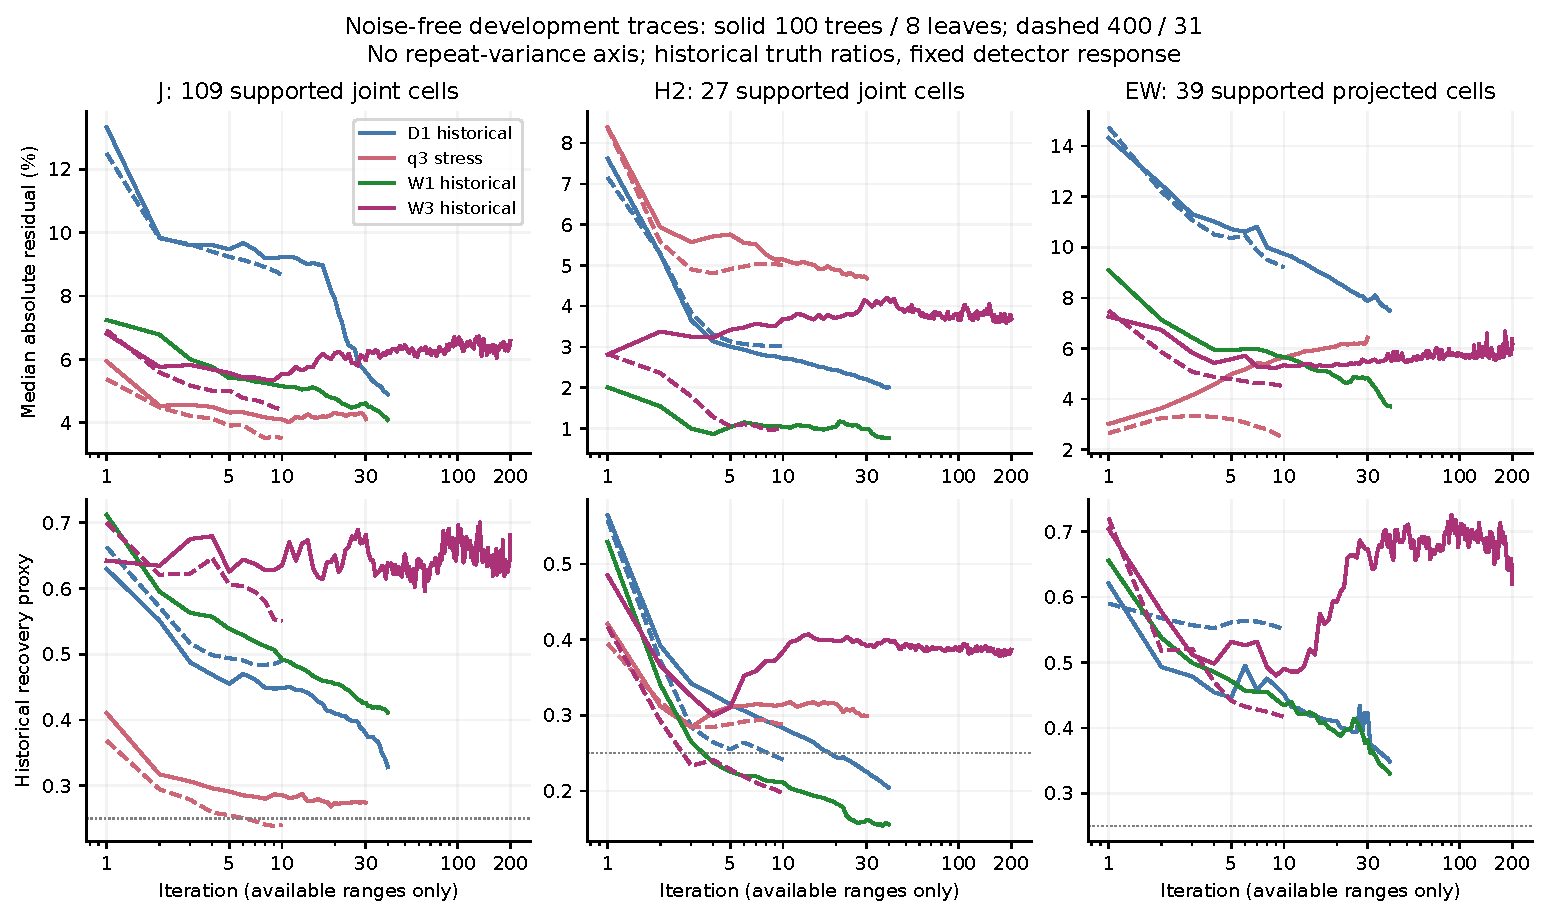
\includegraphics[width=\linewidth]{figures/gbdt_recovery.pdf}

\caption{Noise-free scalar-5D recovery of historical truths at fixed simulated
response. Solid curves use 100 trees/8 leaves; dashed use 400/31 for OmniFold
estimators. D1 and W1 extend to 40 iterations, $q_3$ stress to 30, W3 to 200,
and capacity probes to 10; some baseline traces are partial checkpoints.
The upper row gives median $|\hat f/f_{\rm true}-1|$ over supported cells.
The lower row gives the historical proxy
$\operatorname{median}(|\hat f/f_{\rm true}-1|/|f_{\rm true}/f_0-1|)$
for departures above 1\%, with dotted frozen bound 0.25. Different denominators
prevent interpreting one minus the proxy as an exact recovered fraction.
The $q_3$ stress has no eligible EW departure. These traces measure no repeat variance.}

\label{fig:gbdt-recovery}
\end{figure}

\paragraph{Variability and interval behavior at five iterations.}

Figure~\ref{fig:gbdt-bias-spread} compares ensemble residual means and repeat
standard deviations at the same setting. At historical W3 truth, EW29 has
mean residual \SI{23.67}{\percent} and repeat SD \SI{0.56}{\percent}; EW7 has
\SI{-6.81}{\percent} and \SI{0.30}{\percent}. Small spread does not imply
small bias. Coarser cells can have smaller
residuals and spread, but they estimate different integrals; this is not an improvement
in precision on an unchanged quantity. There are no matching repeat ensembles at
the longer iterations or larger OmniFold capacity from which to infer a tradeoff.

\begin{figure}[tbp]
\centering
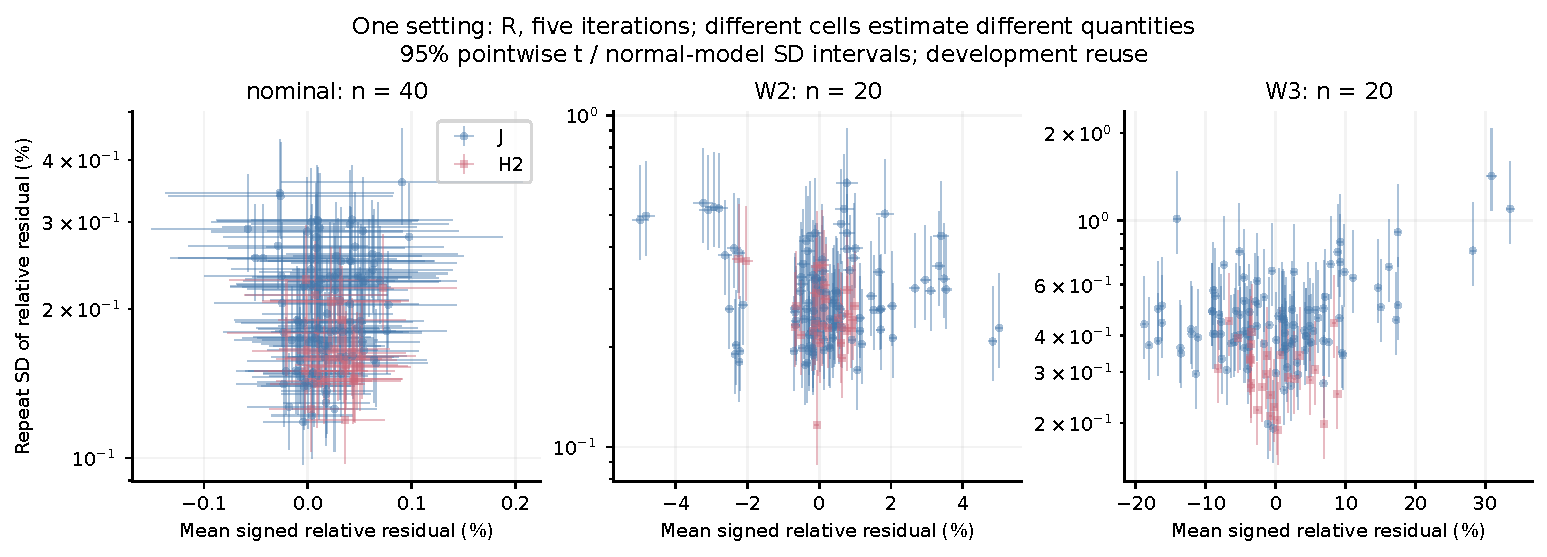
\includegraphics[width=\linewidth]{figures/gbdt_bias_spread.pdf}

\caption{Candidate $R$ at five iterations. Each supported J or H2 cell gives
the mean and SD of $(\hat f-f_{\rm true})/f_{\rm true}$ in the same
background-inclusive ensemble: 40 nominal experiments, 20 each for W2 and W3.
Bars give pointwise 95\% Student-$t$ intervals for means and normal-model
intervals for SDs, conditional on saved simulation. They supply neither
simultaneous bounds nor total uncertainties. Truth panels and reporting cells
form no frontier across estimator settings.}

\label{fig:gbdt-bias-spread}
\end{figure}

Historical statistical intervals fix their width from 100 bootstrap replicas of
one nominal development experiment, without recomputing it per assessment
experiment; their behavior is correspondingly limited
(Fig.~\ref{fig:gbdt-coverage}). Nominal EW41 contains truth in 15
of 40 nominal 68\% intervals (37.5\%, pointwise exact 95\% interval
[22.7\%, 54.2\%]); a pooled calibration pass cannot qualify this cell.
A later 160-experiment check averaged six bootstrap-width estimates. It changed
pull scales without validating the real-data procedure with its own width.
Finite replica noise explains much of the six estimates' apparent variation.
Neither check establishes total coverage.

\begin{figure}[tbp]
\centering
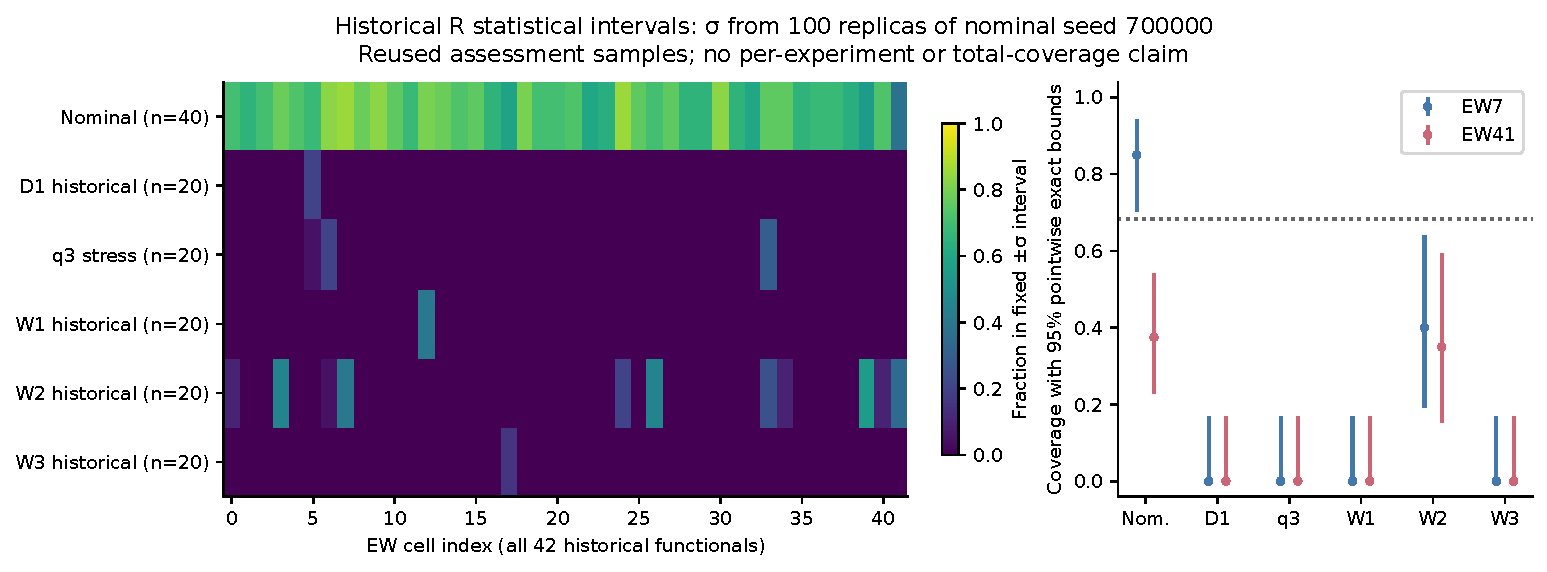
\includegraphics[width=\linewidth]{figures/gbdt_coverage.pdf}

\caption{Development reuse of the historical $R$ assessment: containment in $\hat f\pm\sigma$
with fixed nominal-bootstrap $\sigma$ for all 42 EW functionals. Right shows
EW7 ($\Eavail\in[0.1,0.2)$, $W\in[1.1,1.4)$ GeV) and EW41 (both above
3 GeV), with pointwise 95\% Clopper--Pearson bounds. The dotted line gives
nominal Gaussian 68.27\% coverage. Zero of 20 intervals contains truth;
the upper 95\% bound is 16.8\%, without implying zero population coverage.
Truth ratios are historical. No total-uncertainty construction or newly validated
interval is shown.}

\label{fig:gbdt-coverage}
\end{figure}

A paired perturbation study supports containment of rounding variability for
the tested $R$ refit-per-replica bootstrap. Twenty edge-safe data jitters give
J-cell median SD \SI{0.228}{\percent}, versus bootstrap SD
\SI{0.368}{\percent}. Fifty bootstrap replicas with jittered partners give
median consistency ratio 1.02 and estimated numerical share 0.37 of bootstrap
variance. Adding this share again would double-count it in this design.
The study does not regrade the stability failure, certify interval coverage,
or transfer to the adopted covariance.

\paragraph{Prior sensitivity is not a measured real-data bias.}

Real-data prior shifts correlate with minus the noise-free residual at the same
historical truth (Fig.~\ref{fig:gbdt-prior}). W3's J correlation is 0.92, yet
$|\mathrm{shift}|\geq|\mathrm{residual}|$ holds in only 71\% of supported
cells (52\% on H2, 54\% on EW). Maximum shifts over five historical vertices
have medians 12.0\%, 9.6\% and 13.4\% on J, H2 and EW; excluding D1 gives
11.2\%, 4.3\% and 9.9\%. These sensitivity envelopes provide no probabilities,
covariance components or guaranteed bias bounds. Data truth has not been
demonstrated to lie within their span.

\begin{figure}[tbp]
\centering
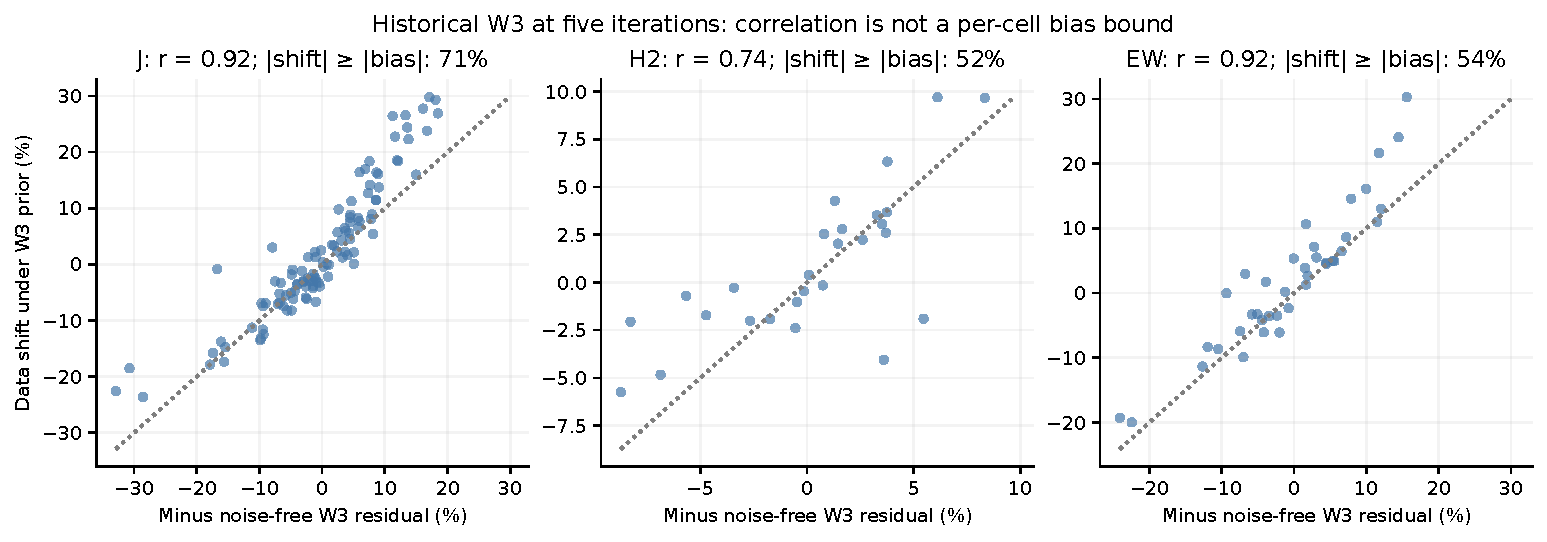
\includegraphics[width=\linewidth]{figures/gbdt_prior_response.pdf}

\caption{Historical W3 at five iterations. Horizontal gives minus the noise-free
relative truth residual; vertical gives the relative shift in real-data $R$
when its MC prior changes to W3, normalized to CV-prior results. Points are
supported cells, not independent repeated experiments. The diagonal marks
equality. Strong correlation supplies no per-cell bound; shifts do not measure
unknown real-data bias.}

\label{fig:gbdt-prior}
\end{figure}

A decisive next measurement would share pseudo-data and MC splits across a small
set of iteration and capacity settings, measuring bias, variance and mean squared
error for common functionals. Comparing settings statistically and validating
intervals are separate tasks. Total-interval validation also requires explicit
physical-nuisance and model-dependence treatment. No new ensemble enters this
synthesis; the precision-measurement objective remains unmet.
% Evidence: nd-unfolding/gbdt_model_dependence/{inputs,results,README.md}; VL163.
% Historical grades: s5e A_FAIL; s5p amendment 4 NOT ADMITTED; amendment 6 LOW corrections.

\subsubsection{Five-dimensional coverage test}
\label{sec:coverage-5d}

An end-to-end independent-truth test assessed statistical intervals of a
deterministic five-dimensional estimator variant with nominal-truth bias
correction (1,200 pseudo-experiments over three truths). It failed its predeclared
futility criterion at the nominal and the $\Eavail$-tilted truths, so no frequentist coverage is
claimed for any five-dimensional interval.

% Source: docs/orchestration/OUTCOME-20260925-s5c-tier-s-futility-fail.md; VALIDATION_LEDGER VL150.

\paragraph{A scoped response-information diagnostic.}
A subsequent signal-only study compared binned exact-response inversions and
local information widths with the stored GBDT residuals. Of 376
joint-cell/departure combinations with residuals above 2\%, 232 changed
classification with truth resolution or response weighting and were excluded.
Among the remaining 144, 121 (84\%) were classified as weakly constrained
under the study's binned, fixed-response assumptions. Thus the result supports
weak response information for that subset, not a universal explanation of
the unfolding residual. The coarser muon projection retained only three cases
and was effectively uninformative. The diagnostic does not bound biased or
unbinned estimators, validate intervals, or establish an impossibility theorem;
its proposed precision thresholds are not scientific adoption gates.
The full exclusions, definitions and numerical verification are in the
\href{https://github.com/josephbaileyy/MINERvA-OmniFold/blob/7d173bd0bad495c4dcbb404ae769cab718fb928c/docs/orchestration/state/next-preparation-20261009/d-id/REPORT.md}{binned response diagnostic record}.

\subsection{Joint five-dimensional generator tests}
\label{sec:joint5d}

A frozen test asks whether each of five predictions---MINERvA Tune~v1,
GENIE~2.12.10 (default and with MEC), NuWro~21.09 and GiBUU~2019---is
compatible with the five-dimensional data, in total (rate and shape together)
and in shape alone: ten tests. Each null $H_0(G)$ is the simple hypothesis that
the calibration simulates: the true cross section equals $G$ on the fine 5D
grid, with Tune~v1's shape and $G$'s finite-MC fluctuations below it (for
Tune~v1 this is $H_0$ exactly). The tests use the 109 supported joint cells (J;
GiBUU: the 72 with $\pPar<\SI{6}{GeV/c}$). Each $p$-value is calibrated by
pseudo-experiments simulated under its null through the unfolding (refinement
refit and five iterations on half the simulation) and stopped by a frozen
sequential rule. The claim $p$ is the largest over declared process-shift and
sub-fine-grid variants, and the decisions use Holm's procedure with a
determinacy rule at familywise level 0.05.

All ten hypotheses are rejected (Table~\ref{tab:joint5d}). Each rejection is
also labelled robust to a larger sub-fine-grid residual ($\kappa=3$, report
only). An independent recomputation of every $p$-value and decision from the
stored products, with the reviewer's own code, agrees on all 1379 compared
rows.

Scheduler time limits removed 224 calibration and 53 power draws, so the $B$ in
Table~\ref{tab:joint5d} counts completed draws only. A report-only recovery
reran exactly those seeds. A determinism check fixed in advance (16 of 16
completed seeds rerun bitwise identically) shows that each recovered draw is
the lost draw, so every submitted draw has now been observed. No recovered draw
reaches the observed statistic in any test, claim variant or $\kappa=3$
variant, so no assignment of the lost draws changes any decision. The closest
margin is 4.6 units of $T$ (GENIE~2.12.10 + MEC shape, $\kappa=3$ variant;
$T_{\rm obs}=868.6$); the next is 49.8 (GENIE~2.12.10 shape). With complete
batches the frozen rule would have stopped Tune~v1, GENIE~2.12.10,
GENIE~2.12.10 + MEC and GiBUU one batch earlier ($B=1200$), with the same
decisions.

The scope of the recovery's checks is narrower than that of the main
recomputation:
\begin{itemize}[itemsep=1pt, topsep=2pt]
  \item its independent cross-check (856 of 856 quantities) covers only the
        reading with the frozen process shifts;
  \item the reading with the shift recomputed on all draws was reproduced only
        by a standalone replay of the same code, a consistency check rather than
        an independent recomputation;
  \item the earlier-stop decisions rest on the campaign's self-validated
        stopping replay.
\end{itemize}
The recovery is report-only: the primary decisions are those of the frozen
evaluation, at the frozen $B$.

Every test rejects, so power is context only. At the Tune~v1 null, two of the
three declared alternatives are detected in shape with power 1.0 at the 0.005
level; the third, a MEC-like shape, with 0.23. At the GENIE~2.12.10 null the
shape powers at 0.005 are 0.74, 0.02 and 0.00. These come from the frozen sets
(172--199 of 200 each). Against the frozen null ensembles, the complete recovered
sets agree within 0.01; with the null recomputed on all draws, GENIE~2.12.10's
first set moves to 0.72.

\begin{table}[htbp]
  \centering
  \small
  \begin{tabular}{@{}lrrcccc@{}}
    \toprule
    Prediction $G$ & $B$ & \multicolumn{2}{c}{$k$ (total, shape)} & \multicolumn{2}{c}{claim $p$ (total, shape)} & Decision \\
    \midrule
    MINERvA Tune~v1       & 1365 & 0 & 0 & $1/1366$ & $1/1366$ & both rejected \\
    GENIE~2.12.10         & 1366 & 0 & 0 & $1/1367$ & $1/1367$ & both rejected \\
    GENIE~2.12.10 + MEC   & 1343 & 0 & 0 & $1/1344$ & $1/1344$ & both rejected \\
    NuWro~21.09           & 1751 & 0 & 1 & $1/1752$ & $2/1752$ & both rejected \\
    GiBUU~2019            & 1351 & 0 & 0 & $1/1352$ & $1/1352$ & both rejected \\
    \bottomrule
  \end{tabular}
  \caption{Joint five-dimensional generator tests. $B$ is the number of completed
  calibration pseudo-experiments at the frozen stop (1400 submitted per null,
  NuWro 1800; the rest were lost to time limits and recovered report-only, see
  text), and $k$ the number at least as extreme as the data; claim
  $p=(k+1)/(B+1)$ is never zero. Holm thresholds run from 0.005 to 0.05; every
  95\% Clopper--Pearson interval for $k/B$ lies below its threshold.}
  \label{tab:joint5d}
\end{table}

These are statements about the simple hypotheses $H_0(G)$, not a measured
cross section. They hold under the test's frozen conditions:
\begin{itemize}[itemsep=1pt, topsep=2pt]
  \item below the fine grid the null carries Tune~v1's shapes; the sub-fine-grid
        check is not converged, and its effect enters as the declared variants
        (the $\kappa=2$ claim variants);
  \item the simulation's per-event detector response beyond the drawn detector
        bands, and a linear surrogate for the five lateral bands; with no
        recoil-energy-scale band, hadronic-response completeness is not established;
  \item the interaction-model prior is the analysis's 34 bands, every band drawn
        per experiment; negative weights in two of them (LowQ2\_1, HighQ2\_1) are
        clipped per universe (at most 0.35\% of a band's shift);
  \item pseudo-experiments unfolded with half the simulation, the data with all
        of it; the resulting shift, at most about 0.05 null standard deviations
        but not always consistent with zero, enters as the bias-aligned
        upper-bound variant;
  \item GiBUU's missing $E_\nu>\SI{20}{GeV}$ component, with its out-of-domain
        truth entering migrations into the tested cells; for all generators,
        $E_\nu>\SI{100}{GeV}$ is absent (negligible);
  \item the predictions' own finite MC, entering the metric as
        $\mathrm{diag}\,\mathrm{Var}(\mu_G)$ and as a drawn residual.
\end{itemize}
No new reportable uncertainty is produced (App.~\ref{app:provenance}, \texttt{joint-5d}).

The grid specifies a finite hybrid hypothesis and reporting statistic; it
does not turn OmniFold's event-level training into binned unfolding.
In the matched coarse muon-only projection, GENIE~2.12.10 CV is not rejected,
whereas its $(\Eavail,W)$ projection is. This post hoc comparison shows that
hadronic information participates in this rejection; it does not establish
added power of the joint test over all matched projections, or accept GENIE
as true. The comparison and its independent recomputation are preserved in
the \href{https://github.com/josephbaileyy/MINERvA-OmniFold/blob/3892e769043cddebfd58ec19e1ab1a567eb01784/docs/publication/w1/W1-RECORD-20261006.md}{matched-projection record}.

The multiplier $\kappa$ scales the last measured refinement change
$\delta_{\rm M1}$: $\kappa=1$ means one such change, not one standard
deviation or a confidence level. A report-only scan first loses determinate
rejection at $\kappa\in(5.2547,5.2563]$ for the frozen ensembles, or
$(5.1688,5.1703]$ with recovered draws included. The first loss is an
undetermined decision, not a determinate failure to reject. This probes one
direction and establishes neither convergence nor a bound on the true
below-grid discrepancy; see the
\href{https://github.com/josephbaileyy/MINERvA-OmniFold/blob/3892e769043cddebfd58ec19e1ab1a567eb01784/publication/kappa/RECORD-20261008-kappa-breakdown.md}{refinement-sensitivity record}.
% Source: docs/orchestration/RECORD-20261005-s5p-joint-5d-inference-result.md (decisions, B, k, p,
% the six conditions verbatim); RECORD-20261006-s5p-lost-seed-recovery-resolution.md (recovery,
% margins 4.6/49.8 T units, earlier stops, power over the complete sets); DECISION-20261005-s5p-
% recompute-extension-and-lost-seed-recovery.md section 5 (Joseph's disposition: certified, margin
% disclosed; the five required disclosures). Wording review: REVIEW-20261006-s5p-stage7-note-wording.md.

\section{Five-dimensional estimator: validation and uncertainty}
\label{sec:5d}

This section validates the five-dimensional estimator behind the central values of \S\S\ref{sec:3d}--\ref{sec:eavailw}. It covers what each test isolates (\S\ref{sec:val-fiveaxis}), background subtraction and generator-sized truth changes (\S\ref{sec:val-negweight}), why the estimator does not follow such changes (\S\ref{sec:val-departure}), model dependence and the reporting definitions it rules out (\S\ref{sec:gbdt-model-dependence}), the coverage test (\S\ref{sec:coverage-5d}) and the status of the five-axis covariance of the configuration-(a) central value (\S\ref{sec:eavailw-construction}). The sixteen-cell result of configuration (e) follows in \S\ref{sec:fived16}, and the calibrated generator tests built on a variant of this estimator in \S\ref{sec:joint5d}. The unbinned negative-weight background method itself is derived in App.~\ref{app:negweight}.

\subsection{Which source of error is being tested}
\label{sec:val-fiveaxis}
Prior reweighting changes the frequencies of existing simulated truth events while retaining their detector-response simulation; a response mismatch instead changes how a given truth is reconstructed. Finite classifier capacity and iteration count approximate the inverse and can leave residuals in either case. Coverage asks whether the resulting intervals contain their specified target at the stated rate (\S\ref{sec:coverage-5d}). These mechanisms are separate: an incorrect generator prediction alone does not diagnose an interval failure. Each test below isolates one intervention.
% Register round n1 (R-N1): the two findings summarized here print at their homes: the refined subtraction's nominal
% recovery in sec:val-negweight and sec:val-departure, and the signal-only result in sec:val-negweight.


All 2D closures in \S\ref{sec:validation} unfold reweighted simulated signal without background, so they do not test background subtraction.

% Methods-paper shortening pass (2026-10-21, DECISION-20261020-joseph-refined-estimator-shorten-delta.md item 2): the article's validation-design table, moved with its sources: 3D/4D closure, sec_validation.tex (thresholds); background closure OUTCOME-20260925-s5c-purity- background-bias-at-high-W.md:1-10 and s5n stage 1; generator-sized change, this section ("predeclared GiBUU-to-GENIE departure screen"); withheld shapes, OUTCOME-20260926-s5e-oi192-diagnosis-and-candidate.md (A4, compared with the adopted sigma); coverage, OUTCOME-20260925-s5c-tier-s-futility-fail.md:30-36; calibration, amendment 7 and sec_joint.tex. REVIEW-1 finding 2: no record that the 3D threshold was set in advance (sec_validation.tex:138-144). The tilt: truth weight 1 + 0.2 (u - 1/2), u = E_avail/100 GeV (nd-unfolding/s5c_pseudo.py:67-70); KNOWN_ISSUES row 98.
\providecommand{\pcell}[2]{\parbox[t]{#1}{\raggedright\strut#2\strut}}
Table~\ref{tab:validation-design-5d} lists the validation studies of the article and of this note (detector response: \S\ref{sec:closure-map} and \S\ref{sec:joint5d-calibration}). Letters refer to Table~\ref{tab:estimators-matrix}.

\begin{table}[htbp]
  \caption{Validation studies of the article and of this note.}
  \label{tab:validation-design-5d}
  \centering\footnotesize
  \begin{tabular}{@{}lllll@{}}
    \toprule
    \pcell{0.17\textwidth}{Study} & \pcell{0.22\textwidth}{Truth change} & \pcell{0.10\textwidth}{Backgrounds} &
    \pcell{0.16\textwidth}{Domain} & \pcell{0.23\textwidth}{Criterion} \\
    \midrule
    \pcell{0.17\textwidth}{Two-dimensional reproduction (f), (a), (b)} & \pcell{0.22\textwidth}{none: data against the publication} &
    \pcell{0.10\textwidth}{data} & \pcell{0.16\textwidth}{205 published bins} & \pcell{0.23\textwidth}{none; descriptive} \\
    \pcell{0.17\textwidth}{Three-, four-observable closure (a)} & \pcell{0.22\textwidth}{injected bump in truth $\Eavail$ (three observables) or $q_{3}$ (four)} &
    \pcell{0.10\textwidth}{none} & \pcell{0.16\textwidth}{one-dimensional marginals} & \pcell{0.23\textwidth}{descriptive: residual ratio 0.10 ($\Eavail$; \S\ref{sec:3d-closure}, \S\ref{sec:closure-map})} \\
    \pcell{0.17\textwidth}{Background closure (c), (d)} & \pcell{0.22\textwidth}{none (nominal truth)} &
    \pcell{0.10\textwidth}{included} & \pcell{0.16\textwidth}{42 $(\Eavail,W)$ and \jtNcells{} joint cells} & \pcell{0.23\textwidth}{none; studies during estimator development} \\
    \pcell{0.17\textwidth}{Generator-sized change (d)} & \pcell{0.22\textwidth}{GiBUU/GENIE $\Eavail$ shape ratio} &
    \pcell{0.10\textwidth}{included} & \pcell{0.16\textwidth}{42 $(\Eavail,W)$ cells} & \pcell{0.23\textwidth}{recovery requirement; not met} \\
    \pcell{0.17\textwidth}{Shapes held out of development (e)} & \pcell{0.22\textwidth}{NuWro and GENIE + MEC shapes, not used while (e) was chosen} &
    \pcell{0.10\textwidth}{included} & \pcell{0.16\textwidth}{42 $(\Eavail,W)$ cells} & \pcell{0.23\textwidth}{compared with the configuration-(a) total $\sigma$} \\
    \pcell{0.17\textwidth}{Coverage (c)} & \pcell{0.22\textwidth}{nominal; signal rate lowered by about 10\% with a weak $\Eavail$ slope (weight 0.900--0.906 below \SI{3}{GeV})} &
    \pcell{0.10\textwidth}{included} & \pcell{0.16\textwidth}{153 cell and projection integrals} & \pcell{0.23\textwidth}{upper bound on coverage at least 0.66 (0.94)} \\
    \pcell{0.17\textwidth}{Test calibration (e)} & \pcell{0.22\textwidth}{each null hypothesis} &
    \pcell{0.10\textwidth}{included} & \pcell{0.16\textwidth}{\jtNcells{} (GiBUU \jtNcellsGiBUU) joint cells} & \pcell{0.23\textwidth}{size set by the calibration (\S\ref{sec:joint5d-frozen})} \\
    \bottomrule
  \end{tabular}
\end{table}

\subsection{Background subtraction and generator-sized truth changes}
\label{sec:val-negweight}

\paragraph{Background subtraction.}

End-to-end five-dimensional pseudo-experiments add background-simulation events and rebuild per-bin purity weights as in the measurement. At nominal truth they return the highest-$W$ column of $(\Eavail,W)$ \SIrange{3.5}{4.1}{\percent} low and the highest-$\Eavail$, highest-$W$ cell \SI{1.7}{\percent} high; without background, the same experiments recover the truth to \SI{0.22}{\percent}. Relative to these cells' total uncertainty in the configuration-(a) covariance, the bias is 0.36--1.07 standard deviations. The bias comes from the purity-based subtraction (\S\ref{app:negweight}), enters no quoted covariance, and has no established size on data. Refined unbinned negative-weight subtraction (App.~\ref{app:negweight}), applied with a deterministic variant of the five-dimensional LightGBM production estimator, brings the highest-$W$ column to \SIrange{0.11}{0.24}{\percent} and the corner cell to \SI{0.24}{\percent} over sixty nominal-truth experiments. Some joint cells remain up to \SI{1.0}{\percent} high, up to 14 standard errors, against \SI{-0.2}{\percent} without background; the mechanism is not established. On data, the two treatments differ by a median of \SI{0.36}{\percent} and at most \SI{1.4}{\percent} over the reported functionals. These differences measure method sensitivity, not bias. Negative-weight subtraction is not used for the configuration-(a) five-dimensional central value; the sixteen-cell result uses it (\S\ref{sec:fived16}).
% (scalar-5D campaign, development study D1)
% Sources: docs/orchestration/OUTCOME-20260925-s5c-purity-background-bias-at-high-W.md,
% docs/orchestration/state/s5c/d1/d1_summary.json, docs/orchestration/state/s5c/d1/bias_vs_adopted.json.
% CLI form: \texttt{-{}-bkg-mode negweight-refined}. Implementation (refinement to
% non-negative weights before the first OmniFold step; injection and independent
% subtraction halves of the background simulation) is in the negative-weight appendix (app:negweight).

\paragraph{Generator-sized truth changes.}

The unfolding does not follow a GiBUU-to-GENIE $\Eavail$ shape reweighting of the truth (0.70--1.33 per $\Eavail$ bin, total preserved). The GENIE prediction behind the ratio uses a mis-sampled flux (\S\ref{sec:3d-models}), so the ratio is a valid known-truth deformation of generator size but not a measured GiBUU--GENIE difference. The $(\Eavail,W)$ residuals have a median of \SI{9.7}{\percent}; they reach \SI{74}{\percent} in the highest-$W$ column and several percent in the largest cells. The \SI{74}{\percent} residual is in the cell $0.8\le\Eavail<\SI{1.5}{GeV}$, $W\ge\SI{3}{GeV}$, whose share of the cross section the deformation study did not record. A $q_3$ deformation preserving the $(\Eavail,W)$ truth shifts these cells by up to \SI{37}{\percent}. Signal-only experiments with the same seeds reproduce both results. The residuals are therefore a property of the estimator (five iterations, the GBDT configuration of \S\ref{sec:method}), not of the background treatment; their status in the quoted uncertainties is given in \S\ref{sec:val-departure}.
% KNOWN_ISSUES.md row 83
% Register round r12 (2026-10-21): the cell and the unrecorded share moved from the article's Sec. V B; source
% figures/methods_m3/fig_m3_deformation.py numbers output (EW29); dev_receipt.json and truth_check.json carry no yields.
% Register round n1 (R-N1): the status of this bias (it enters no quoted uncertainty) is stated once, at its home in
% sec:val-departure.
% Source: docs/orchestration/OUTCOME-20260925-s5n-stage1-development-fail.md (VL151, VL152);
% KNOWN_ISSUES 75, 77; independently reproduced (state/s5n/stage1/review-round-1.md).

\subsection{Why the estimator does not follow a generator-sized change}
\label{sec:val-departure}
% An instrumented rerun recorded every OmniFold iteration of these experiments. It reproduced the development results bitwise and repeated them through the unmodified driver, which shows the same response to the $\Eavail$ departure (highest-$W$ cell
% \SI{73.8}{\percent} against \SI{73.5}{\percent}).

Both OmniFold steps behave as intended: the first matches the reconstructed pseudo-data within statistical noise, and the second reproduces the truth-level weight sums to \SI{0.5}{\percent}. Yet the unfolded result folds back onto the data less well than the true model does. With noise-free pseudo-data the unfolding recovers more than \SI{99}{\percent} of the change that the departure produces in the reconstructed distribution, whereas the median $(\Eavail,W)$ truth residual ranges from \SI{5}{\percent} to \SI{11}{\percent}, with \SI{74}{\percent} in the worst cell. The unrecovered reconstructed-level difference is small relative to the departure but statistically significant at the analysis exposure.

With noise-free pseudo-data, thirty iterations reduce the $\Eavail$ residual by \SI{26}{\percent}; the $\Eavail$ residual continues to fall slowly, while the $q_3$ residual grows with iterations. A larger classifier improves the reconstructed-level fit without reducing the $\Eavail$ truth residual, and removing the regression for events that fail reconstruction does not reduce that residual either. No single cause is established, and no estimator change within the scope of the study meets the recovery requirement, set before the test, for the GiBUU-to-GENIE departure. The $\Eavail$ and $q_3$ residuals, a regularization (unfolding-model) bias of the estimator, enter no uncertainty quoted for the configuration-(a) central value. For the sixteen-cell result (\S\ref{sec:fived16}), the model term of the reported covariance is the change in the unfolded data when the prior is reweighted to each generator (GENIE + MEC, NuWro, GiBUU; \S\ref{sec:fived16-cov}). This term is unscaled and is not a calibrated bound. The fake-data study of \S\ref{sec:fived16-fd} measures the estimator's bias and compares it with the reported covariance.
% Register round n1 (R-N1, R-N6): the home of the residual-bias statement (moved from sec:val-negweight); "that the
% study's rules allow" stated as its scope (OUTCOME-20260926-s5e-oi192-diagnosis-and-candidate.md:43, "no authorized
% estimator change passes its predeclared screen").

% CLAIM-ADDITION D-ID BEGIN Register round 2 (methods paper, 2026-10-21), claim addition for Joseph, to be committed separately. Source: docs/orchestration/state/next-preparation-20261009/d-id/REPORT.md (simulation-only; NOT CITABLE FOR a coverage result or an interval, :7-13). Setting: T2, same-sample, nominal-weighted, K = 5, pooled over GiBUU (= D1), W1, W3, q3 and W2 (:394); the IBU starts from the nominal prior (:74) with exact efficiency (:183-186); reco binning 10,499 cells (:97, :382); W2's comparator is background-inclusive and the outcome is unchanged without it (:398, :204-207, :559). J medians at K = 5 (:432-440). Eligible 144, approximation-dominated 15, 2 identified, A share 0.014 (:398, :430-431, :530-532). C-counted 121 of 144, CR widths > 10% at both truth resolutions, median 31% at T1 = the J cells (:70-71, :416-423, :516-518); "the regularization trades a large variance for the bias" (:524-529). Long iteration: K = 200 and 1e5 medians (:441-451), binning bias growing for W3 and q3 (:451), no run-level convergence, 9-34 of 109 J functionals converged (:452-455, :553-555). Scope: :5-13, :412-415 (38% of the > 2% population), :547-565. Conclusion: :524-534.
\paragraph{Comparison with exact binned unfolding.} A diagnostic in simulation compares the boosted-tree residual with that of an exact binned iterative unfolding. The binned unfolding unfolds the same simulated events, with their exact efficiency and the response binned in the 10,499 occupied five-dimensional reconstructed cells, starting from the nominal prior. The comparison uses noise-free signal-only pseudo-data, the 109 supported fine joint cells (J cells) and the fixed historical truth deformations D1, W1, W3 and the $q_3$ stress, pooled with W2 (all defined in \S\ref{sec:gbdt-model-dependence}). The boosted-tree comparator for W2 includes background; the outcome is unchanged without it. A residual is eligible when its diagnosis is stable under the truth resolution: of the 376 J-cell and deformation combinations with residuals above \SI{2}{\percent}, 232 changed classification with the truth resolution or the response weighting and were excluded, leaving 144 (\SI{38}{\percent} of the 376). At five iterations the J-cell medians of the absolute residual agree: \SI{9.5}{\percent}, \SI{5.4}{\percent}, \SI{5.6}{\percent} and \SI{4.3}{\percent} for the boosted trees, against \SI{8.3}{\percent}, \SI{5.4}{\percent}, \SI{4.9}{\percent} and \SI{5.3}{\percent} for the exact binned unfolding, for D1, W1, W3 and the $q_3$ stress. Of the 144 eligible residuals, pooled over the deformations, 15 are dominated by the tree approximation. Only 2 of these 15 lie in identified quantities (as defined in the diagnostic record cited below), a share of 0.014 of the 144. Of the 144, 121 lie in quantities that the binned response constrains weakly at the analysis exposure. Their Cram\'er--Rao widths exceed \SI{10}{\percent} at both truth resolutions tested (median \SI{31}{\percent} at the coarser resolution, that of the J cells themselves), so the regularization trades a large variance for the bias. Longer noise-free exact iteration removes much of the residual for D1 (J median \SI{3.3}{\percent} after 200 iterations and \SI{0.8}{\percent} after $10^{5}$) and part of it for W1 (\SI{3.3}{\percent} and \SI{2.8}{\percent}). It does not do so for W3 and the $q_3$ stress (\SI{4.4}{\percent} and \SI{6.6}{\percent} after 200 iterations, \SI{8.9}{\percent} and \SI{6.7}{\percent} after $10^{5}$), whose within-cell binning bias grows with the iteration number. The long runs do not converge (only 9--34 of the 109 J quantities converge for each traced deformation), so these values are last iterates. The coarser muon projection retained only three cases and is uninformative. Within this comparison, the residual is consistent with the regularization of the inverse problem at this binning and prior, and the tree approximation is not supported as its main cause. This conclusion holds for a binned, signal-only and noise-free comparison at the simulation's detector response, on the development truths, and for these 144 residuals only. It does not address what unbinned or biased estimators could recover, the coverage failure of \S\ref{sec:coverage-5d} or the validity of any interval, and it establishes no impossibility. The precision thresholds that the diagnostic proposes are not acceptance criteria for any result in this note. The exclusions, definitions and numerical verification are in the binned response diagnostic record (Ref.~\cite{NoteRecords2026}, \recentry{response-diagnostic}).
% Register round r12 review (S6): the 200-iteration W3 and q3 medians added from the binned response diagnostic
% record (d-id REPORT.md, longer exact iteration table: J median of |r_IBU| at K = 200, nominal-weighted T2).
% CLAIM-ADDITION D-ID END

\paragraph{Higher-capacity background refinement and data stability.}

The refinement classifier underfits, which causes the residual background bias (App.~\ref{app:negweight}). A candidate with raised refinement capacity, configuration (e) of the sixteen-cell result (\S\ref{sec:fived16}), passes the nominal background-inclusive closure on 40 fresh pseudo-experiments (largest deviation 2.7 standard errors) and a pooled test of its statistical intervals (pull width 1.02). The pooled test does not establish coverage and width for every functional. The candidate fails the data-stability test, whose criterion was set before it was run: input perturbations within floating-point rounding move functionals by a median of 0.8 and at most 2.6 statistical standard deviations. The baseline estimator's shifts, a median of 0.8 and at most 2.5, place this instability in the estimator family. The instability also explains the difference of at most \SI{1.2}{\percent} on data between the driver and the development pipeline. The data bootstrap, which refits the full chain per replica, already includes this rounding-level variability: each replica carries the same spread (median \SI{0.23}{\percent} per joint cell), about \SI{37}{\percent} of the bootstrap variance and below a tenth of any total uncertainty. Central values are therefore reproducible only to within this spread. The paired perturbation study of \S\ref{sec:gbdt-model-dependence} tests whether the bootstrap contains this variability, for this candidate only.
% Source: KNOWN_ISSUES 80; docs/orchestration/RECORD-20260927-s5p-stage2-exit.md section 2 (VL155).

\paragraph{Unfolding-model dependence.}

For historical shapes held out while this candidate was assessed (NuWro; GENIE with enhanced meson-exchange currents), its unfolding-model dependence is median \SIrange{2}{6}{\percent} and at most \SIrange{16}{31}{\percent}, within the configuration-(a) total uncertainty in 20 of the 42 $(\Eavail,W)$ cells. No uncertainty from this assessment is used for a quoted result.
% Source: docs/orchestration/DIAGNOSIS-20260926-s5e-oi192-estimator.md (VL153);
% docs/orchestration/OUTCOME-20260926-s5e-oi192-diagnosis-and-candidate.md (VL154); KNOWN_ISSUES 75, 77, 79, 80;
% independently reproduced (state/s5e/diag/review-round-1.md, state/s5e/cand/review-round-2.md).

\subsection{Model dependence, variability and reporting resolution}
\label{sec:gbdt-model-dependence}

The scalar five-dimensional estimator studied here uses production LightGBM.

These studies measure three different quantities: truth-dependent responses to iterations and capacity, small repeat variability at one setting, and appreciable prior sensitivity. Unfolding benchmarks also assess these quantities separately~\cite{Brenner2020Unfolding}. The studies do not establish a bias--variance tradeoff across estimator settings, and regularization bias can invalidate intervals based solely on estimator variability~\cite{Kuusela2015Unfolding}; neither reference supplies the variance measurement that is missing for this estimator.

The noise-free study unfolds the full simulation's reweighted reconstructed events without background. Baseline classifiers and the missed-event regressor use 100 trees and 8 leaves; the capacity probe uses 400 trees and 31 leaves. Repeated experiments use estimator $R$, the raised-refinement-capacity candidate of \S\ref{sec:val-departure}: five iterations, baseline OmniFold estimators and a separate 400-tree, 31-leaf background-refinement classifier. With seed 42, its 40 nominal experiments and 20 at each of five departures include Poisson pseudo-data, changing MC splits and background refinement. These experiments are not an independent validation: their samples were used during development, and their assessment seeds, although separate, were later also used in the estimator's development.
% Register round r18 (S3, director ruling 2026-10-25): moved from the methods paper's Fig. 3 caption ("Panel (b) uses
% separate seeds, which were later also used in the estimator's development"; before r16, "separate assessment seeds,
% which also entered its later development", commit a6b9c705's "assessment seeds, since used in development";
% figures/methods_m3/fig_m3_deformation.py:9, "fresh assessment seeds").

Saved fine-grid outputs are integrated into the supported J, H2 and EW cells of the table below. Unsupported cells remain in the full-domain rate. The interval assessment keeps all 42 EW cells, including the three that the support rule excludes (definitions and normalization checks in App.~\ref{sec:gbdt-diagnostic-definitions}).

\begin{center}
\small
\begin{tabular}{@{}lp{0.72\textwidth}@{}}
\toprule
Label & Meaning in this section \\
\midrule
J & 109 supported fine joint cells, subdividing all five axes \\
H2 & 27 supported coarser joint cells, also subdividing all five axes, not nested within J \\
EW & 39 supported $(\Eavail,W)$ cells (42 with the three unsupported cells) \\
RD1--RD3 & reporting definitions at J, H2 and EW resolution (``Reporting definitions'' below) \\
D1, W1--W3 & fixed historical truth deformations (next paragraph) \\
$R$ & the raised-refinement-capacity estimator of \S\ref{sec:val-departure}: baseline OmniFold classifiers with a 400-tree, 31-leaf background-refinement classifier \\
\bottomrule
\end{tabular}
\end{center}

The truth labels denote fixed historical deformations, built before the generator flux was repaired: D1 is a GiBUU/GENIE $\Eavail$ ratio, W1 a NuWro/GENIE $\Eavail$ ratio, W2 a GENIE MEC/CV $(\Eavail,W)$ ratio, and W3 a NuWro/GENIE $(\pT,\pPar,\Eavail)$ ratio. Excluding D1 does not make the others corrected generator comparisons. The $q_3$ stress changes the conditional distribution at fixed $(\Eavail,W)$ with amplitude 0.3.

\paragraph{Recovery changes, but not uniformly.}

Figure~\ref{fig:gbdt-recovery} shows the traces over the recorded iteration ranges (later checkpoint entries are excluded, App.~\ref{sec:gbdt-diagnostic-definitions}); none is extrapolated. D1 and W1 improve slowly. W3's J-cell median absolute residual rises from \SI{5.57}{\percent} at iteration 5 to \SI{6.57}{\percent} at 200, and its maximum from \SI{32.9}{\percent} to \SI{44.8}{\percent}. The corresponding H2 medians are \SI{3.42}{\percent} and \SI{3.68}{\percent}. The persistence of the W3 residual is established over this finite scan only, not for unlimited iterations or for every possible classifier. The $q_3$ stress shows how much the functional matters: its EW median residual rises from \SI{4.99}{\percent} at iteration 5 to \SI{6.42}{\percent} at 30 even while some joint-cell summaries improve. The capacity probe changes recovery. At five iterations, the most the computing budget allowed at that capacity, the larger classifiers lower the largest residual proxy over the development truths (lower row of Fig.~\ref{fig:gbdt-recovery}) by 3\% on J and 8\% on H2, short of the improvement of at least 20\% required before the larger capacity would be used. The joint-test estimator keeps five iterations under a rule fixed before the comparison. The rule would have replaced five iterations by 10, 15 or 20 only if one of these lowered its measure of model dependence, the largest residual proxy over the development truth changes, on the J or the H2 cells. None did. Because the measure is a maximum over the truth changes, the slow gains for D1 and W1 do not lower the measure: on H2, over the noise-free traces of Fig.~\ref{fig:gbdt-recovery}, it is 0.314 at five iterations and at least 0.384 at 10, 15 or 20. The sixteen-cell result is reported on the same H2 grid after a purity merge of its supported boxes, with total uncertainties (\S\ref{sec:fived16-result}).
% Register round r12 (2026-10-21): the rule moved from the article's Sec. III; source
% RECORD-20260927-s5p-stage2-exit.md sec. 3 (configuration 2, k in 10, 15, 20 against k = 5).
% Note register batch b3 (2026-10-21): the rule scoped by its own measure. RECORD-20260927-s5p-stage2-exit.md
% sec. 2 K (":76-78": M is the maximum over the development alternatives of the T2 proxy, at J and H2) and sec. 3
% (":114-116": the minimizer of M_H2 over k in {10, 15, 20}, 0.384, does not improve on k = 5, 0.314, for J or H2).
% Search: five-dimensional measurement; measurement production; reporting definition; total uncertainties (RECORD-20260927-s5p-stage2-exit.md:1, :141, :171, "no measurement production is admitted", for the precision study's reporting definitions RD1-RD3; re-searched on 8b0f83fd with the five-observable integration applied: the one five-dimensional measurement with total uncertainties the note prints is the sixteen-cell result of sec_fived16.tex, which is not one of RD1-RD3) @ 8b0f83fd
% Deposit pass: the governance wording of these sentences restated as criterion, value and outcome (old text in git
% history). Criterion and value: RECORD-20260927-s5p-stage2-exit.md sec. 3, configuration 3 (capacity at the
% affordable k = 5 lowers M by 8% on H2 and 3% on J, against the rule's 20%; K_afford is 5 iterations at 400/31).

\paragraph{Reporting definitions for a five-dimensional measurement.} The five-dimensional precision study assessed three reporting definitions at the development resolution: the 109 J cells (RD1), the 27 H2 cells (RD2) and the 39 EW cells (RD3). Its bounded unfolding-model component, the largest shift over five generator-sized truth departures at the smallest envelope the vertices allow, has median \SI{12.0}{\percent}, \SI{9.6}{\percent} and \SI{13.4}{\percent} respectively (90th percentile 38.6, 22.5 and \SI{39.2}{\percent}), with GiBUU the dominant vertex in most cells. The study set its total-width target, a median 68\% half-width of at most \SI{10}{\percent}, and its selection procedure before it was run. The study adds the model component linearly to the probabilistic half-width, cell by cell. The model component alone therefore exceeds the total-width target in RD1 and RD3, and in RD2 the target is exceeded once the flat \SI{1.4}{\percent} normalization is added (median at least \SI{11.0}{\percent}). The model-component target, a median of at most \SI{5}{\percent}, and the recovery target, recovery of at least 75\% of a generator-sized departure (a residual proxy of Fig.~\ref{fig:gbdt-recovery} of at most 0.25, against 0.31--0.63 measured), fail in every definition. The selection procedure then takes RD3 as the fallback, and RD3 fails the total-width target. None of the three reporting definitions can meet these precision targets with any estimator configuration the study's selection procedure permits within its computing budget. The limitation is the measured prior dependence, about 10--13\% per coarse joint cell, which is comparable to the generator differences a user would need to resolve. It motivates the calibrated joint tests of \S\ref{sec:joint5d}, a separate inference that reports no measured cross section.
% Register round n1 (R-N6): "fixed before the study" (twice) stated once, as the targets' and the procedure's timing.
% Methods-paper rewrite draft 6 (REVIEW-2 finding 9): RECORD-20260927-s5p-stage2-exit.md:133-135 (half-width = sigma_prob + h).
% plain-language pass 2, director ruling on base defect sec_5d-31-63 (DECISION-20261018-joseph-plain-language-pass2)
% Base read "recovery of at least 75% of a generator-sized departure, against 0.31--0.63 measured", which reads
% as 31-63% recovered. RECORD-20260927-s5p-stage2-exit.md:76-78 (the T2 proxy is the median over reported cells
% with a >1% departure of |bias|/|departure|; M is its maximum over the development alternatives) and :96, :138
% ("0.25 against the measured 0.31-0.63"): 0.31-0.63 is the measured residual proxy M, whose target is <= 0.25.
% Source: docs/orchestration/RECORD-20260927-s5p-stage2-exit.md sec. 4 (VL155). Added 2026-10-11: the article's
% Sec. VII states this result, and the note carried only the one-line verdict above.

\begin{figure}[tbp]
\centering
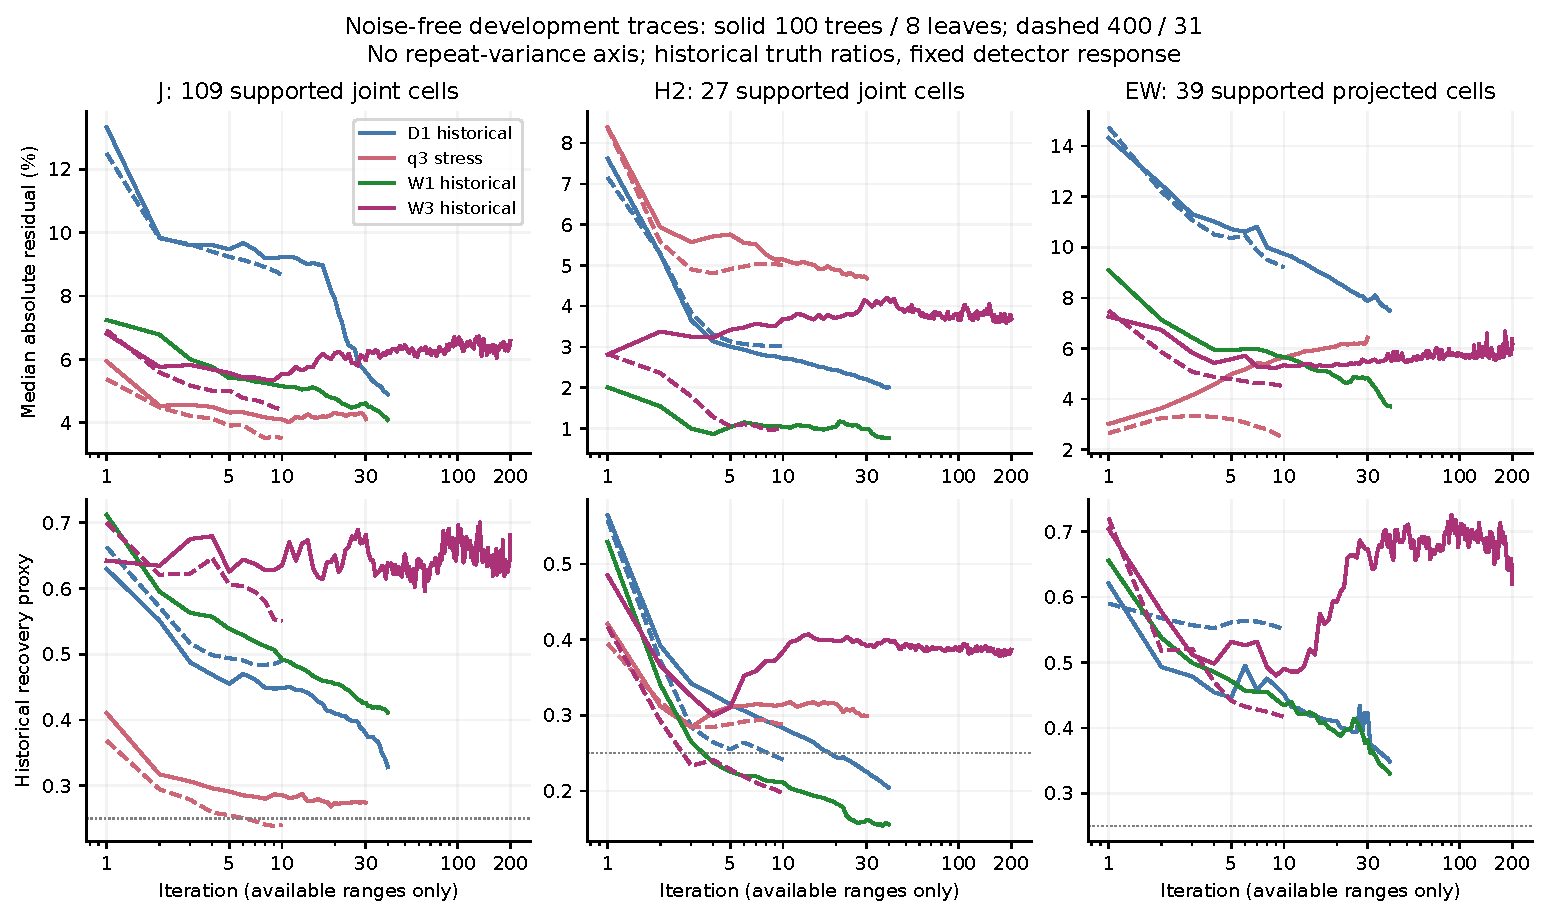
\includegraphics[width=\linewidth]{figures/gbdt_recovery.pdf}

\caption{Noise-free five-dimensional recovery of historical truths at fixed simulated response. Solid curves use 100 trees/8 leaves; dashed use 400/31 for OmniFold estimators. D1 and W1 extend to 40 iterations, $q_3$ stress to 30, W3 to 200, and capacity probes to 10; some baseline traces end at their last saved checkpoint. The upper row gives median $|\hat f/f_{\rm true}-1|$ over supported cells. The lower row gives the study's residual proxy $\operatorname{median}(|\hat f/f_{\rm true}-1|/|f_{\rm true}/f_0-1|)$ for departures above 1\%, with the required bound 0.25 dotted. Different denominators prevent interpreting one minus the proxy as an exact recovered fraction. The $q_3$ stress has no eligible EW departure. These traces measure no repeat variance.}

\label{fig:gbdt-recovery}
\end{figure}

\paragraph{Variability and interval behavior at five iterations.}

Figure~\ref{fig:gbdt-bias-spread} compares ensemble residual means and repeat standard deviations at the same setting. At historical W3 truth, EW29 has mean residual \SI{23.67}{\percent} and repeat SD \SI{0.56}{\percent}; EW7 has \SI{-6.81}{\percent} and \SI{0.30}{\percent}. Small spread does not imply small bias. Coarser cells can have smaller residuals and spread, but they estimate different integrals, so their smaller residuals and spread are not an improvement in precision on an unchanged quantity. No matching repeat ensembles exist at more iterations or larger OmniFold capacity, so no tradeoff can be inferred.

\begin{figure}[tbp]
\centering
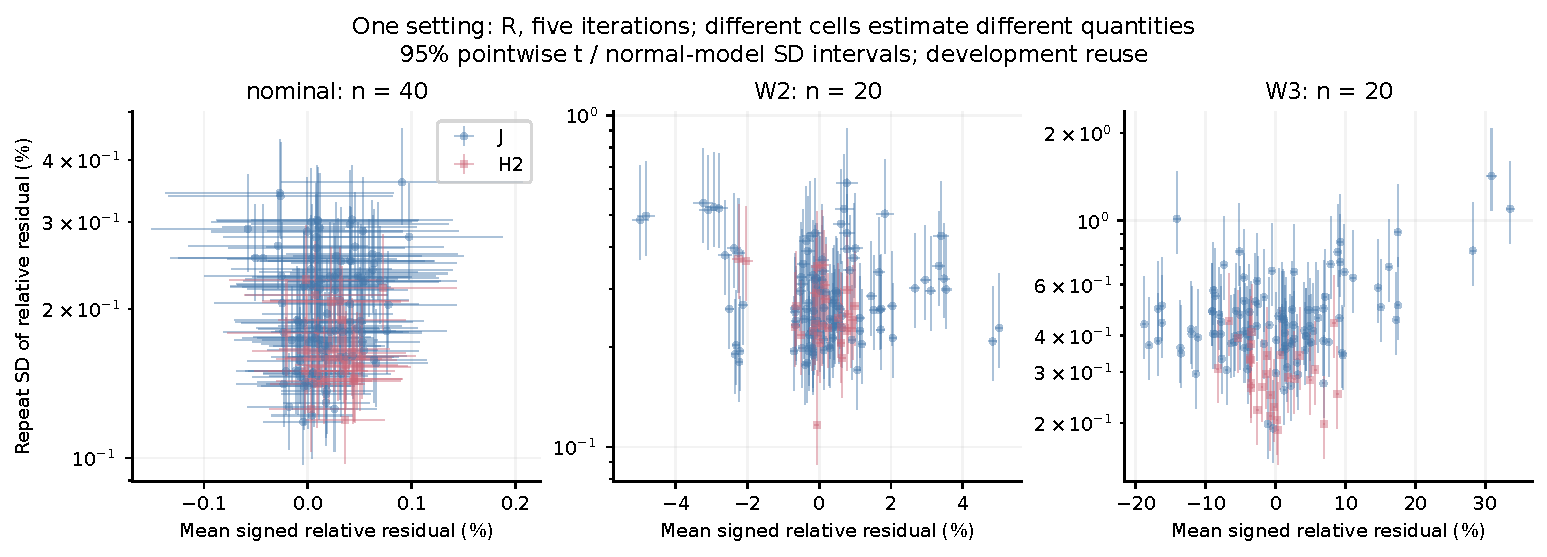
\includegraphics[width=\linewidth]{figures/gbdt_bias_spread.pdf}

\caption{Estimator $R$ at five iterations. Each supported J or H2 cell gives the mean and SD of $(\hat f-f_{\rm true})/f_{\rm true}$ in the same background-inclusive ensemble: 40 nominal experiments, 20 each for W2 and W3. Bars give pointwise 95\% Student-$t$ intervals for means and normal-model intervals for SDs, conditional on saved simulation. They supply neither simultaneous bounds nor total uncertainties. Truth panels and reporting cells form no frontier across estimator settings.}

\label{fig:gbdt-bias-spread}
\end{figure}

The statistical intervals of the development assessment take their width from 100 bootstrap replicas of one nominal development experiment and do not recompute it for each assessment experiment (Fig.~\ref{fig:gbdt-coverage}). At nominal truth, EW41 contains the truth in 15 of 40 68\% intervals (37.5\%, pointwise exact 95\% interval [22.7\%, 54.2\%]), so a pooled pass cannot qualify this cell. A 160-experiment check with the width averaged over six bootstrap estimates changes the pull scales but does not validate the real-data procedure, which uses the data's own width. Finite replica noise explains much of the apparent variation among the six estimates.
% Register round n1 (R-N1): "Neither check establishes total coverage" is covered by the one statement in
% sec:coverage-5d that no frequentist coverage is claimed for any five-dimensional interval.

\begin{figure}[tbp]
\centering
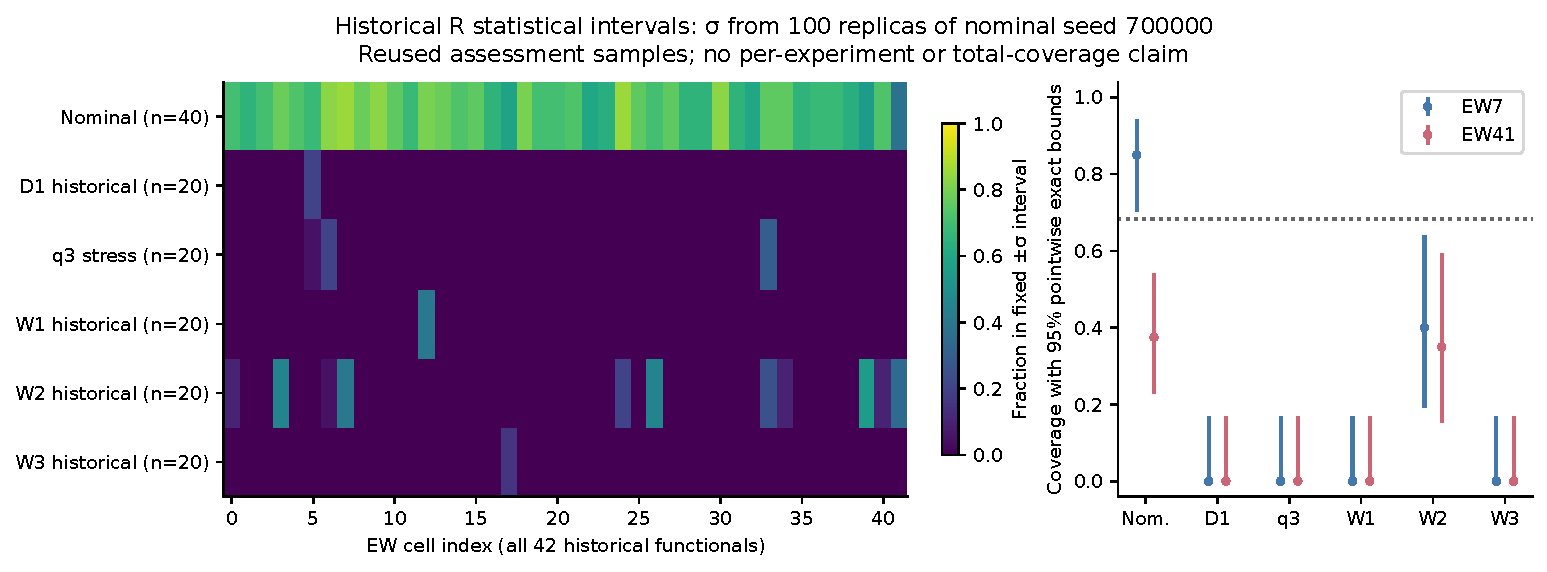
\includegraphics[width=\linewidth]{figures/gbdt_coverage.pdf}

\caption{Development assessment of $R$: containment of the truth in $\hat f\pm\sigma$, with $\sigma$ fixed from the nominal bootstrap, for all 42 EW functionals. Right shows EW7 ($\Eavail\in[0.1,0.2)$, $W\in[1.1,1.4)$ GeV) and EW41 (both above 3 GeV), with pointwise 95\% Clopper--Pearson bounds. The dotted line gives nominal Gaussian 68.27\% coverage. Zero of 20 intervals contain the truth; the upper 95\% bound is 16.8\%, which does not imply zero population coverage. The truth ratios are the historical deformations. No total uncertainty or newly validated interval is shown.}

\label{fig:gbdt-coverage}
\end{figure}

A paired perturbation study supports the containment of rounding variability in the refit-per-replica bootstrap of $R$. Twenty edge-safe data jitters (uniform input perturbations within half a single-precision unit in the last place that keep the fine-grid membership fixed) give a J-cell median SD of \SI{0.228}{\percent}, against a bootstrap SD of \SI{0.368}{\percent}. Fifty bootstrap replicas with jittered partners give a median consistency ratio of 1.02 and an estimated numerical share of 0.37 of the bootstrap variance. In this design, adding the numerical variance to the bootstrap variance would count it twice. The stability failure and the study's scope are in \S\ref{sec:val-departure}, interval coverage in \S\ref{sec:coverage-5d}.

\paragraph{Prior sensitivity is not a measured real-data bias.}

Real-data prior shifts correlate with minus the noise-free residual at the same historical truth (Fig.~\ref{fig:gbdt-prior}). For W3 the correlation over J cells is 0.92, yet $|\mathrm{shift}|\geq|\mathrm{residual}|$ holds in only 71\% of supported J cells (52\% of H2 cells, 54\% of EW cells). Maximum shifts over five historical vertices have medians 12.0\%, 9.6\% and 13.4\% on J, H2 and EW; excluding D1 gives 11.2\%, 4.3\% and 9.9\%. These envelopes are sensitivities: they provide no probabilities, covariance components or guaranteed bias bounds, and the truth of the data has not been shown to lie within their span.

\begin{figure}[tbp]
\centering
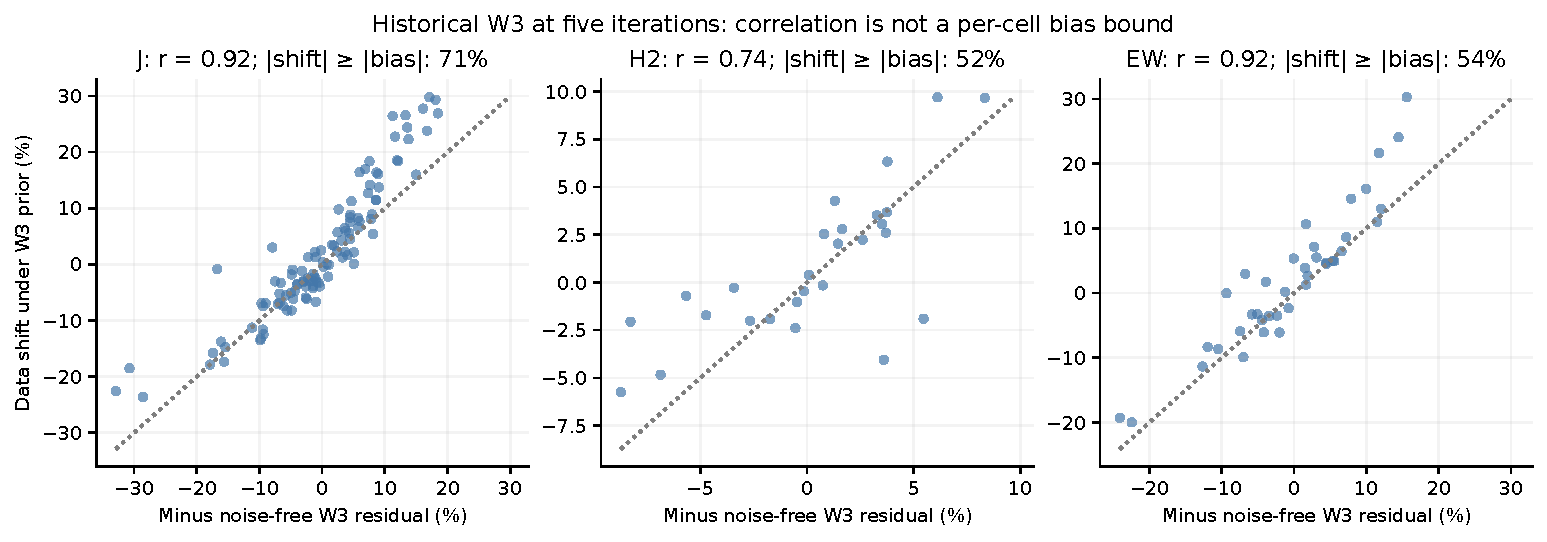
\includegraphics[width=\linewidth]{figures/gbdt_prior_response.pdf}

\caption{Historical W3 at five iterations. Horizontal gives minus the noise-free relative truth residual; vertical gives the relative shift in real-data $R$ when its MC prior changes to W3, normalized to CV-prior results. Points are supported cells, not independent repeated experiments. The diagonal marks equality. Strong correlation supplies no per-cell bound; shifts do not measure unknown real-data bias.}

\label{fig:gbdt-prior}
\end{figure}

Deciding the tradeoff would require sharing pseudo-data and MC splits across a small set of iteration and capacity settings and measuring bias, variance and mean squared error for common functionals. That comparison would not validate intervals, which also requires an explicit treatment of physical nuisances and model dependence. No new ensemble enters these studies.
% Evidence: nd-unfolding/gbdt_model_dependence/{inputs,results,README.md}; VL163.
% Historical grades: s5e A_FAIL; s5p amendment 4 NOT ADMITTED; amendment 6 LOW corrections.

\subsection{Five-dimensional coverage test}
\label{sec:coverage-5d}

An end-to-end independent-truth test assessed statistical intervals of a deterministic five-dimensional estimator variant with nominal-truth bias correction (1,200 pseudo-experiments over three truths). It failed its futility criterion, set before the test was run, at the nominal truth and under a 10\% reduction of the signal rate with a weak $\Eavail$ slope (below). No frequentist coverage is therefore claimed for any five-dimensional interval. Figure~\ref{fig:coverage-5d-paper} shows the coverage of each reported integral under the rate reduction. The intervals divide each estimate by $1+\beta$, where $\beta$ is the relative closure bias at nominal truth, and add the standard error of $\beta$ times the corrected estimate in quadrature to the statistical standard deviation. A quantity fails when the upper confidence bound on its coverage lies below 0.66 for 68\% intervals or below 0.94 for 95\% intervals. The second truth (the $\Eavail$ tilt) multiplies the true signal by $1+0.2\,(\Eavail/\SI{100}{GeV}-\tfrac12)$ without renormalization, with the background unchanged; below $\Eavail=\SI{3}{GeV}$ the weight is 0.900--0.906. Under that change, 51 of the 153 reported cell and projection integrals have 68\% coverage confidently below nominal, with coverage as low as 0.060, and 42 of the 153 fail at 95\%. At nominal truth two of the 153 fail at 95\%, the lowest coverage being 0.850.
% Register round n1 (R-N1, R-N6): the one statement of the five-dimensional interval status, for all of sec:5d;
% "predeclared" (here) and "fixed in advance" (Table tab:validation-design-5d) stated once, as the criterion's timing.
% plain-language pass 2 (DECISION-20261018-joseph-plain-language-pass2): theme A, note home for the paper's
% Sec. IV C numbers. Source: OUTCOME-20260925-s5c-tier-s-futility-fail.md:30-36 (table: nominal 0 / 2 futile,
% min 0.570 / 0.850; E_avail tilt a=0.2 51 / 42 futile, min 0.060 / 0.288; UCB < 0.66 / < 0.94; per-comparison
% level 0.05/459) and :41-43; receipt state/s5c/tier_s/interim_400.json (aa574c17...): 153 functionals =
% 109 J cells + 42 EW cells + the EW all-ones sum + the total integrated rate.
% Methods-paper rewrite draft 5: the interval definition, moved here from the article (nd-unfolding/s5c_coverage.py:77-80).
% Draft 6 (REVIEW-2 finding 13): nd-unfolding/s5c_coverage.py:79-80, half-width z sqrt(sigma^2 + (se f)^2).
% Methods-paper rewrite draft 4 (X5 G5b, verified by the director): nd-unfolding/s5c_pseudo.py:67-70 (weight),
% :125-128 (applied to the pseudo-data signal, not renormalized; background unchanged); KNOWN_ISSUES row 98.

\paragraph{Why the intervals miscover under the rate reduction.} The diagnosis below uses the stored outputs and the code.  The rate change itself is recovered: in the one locally stored pseudo-experiment the total changes by \SI{-9.58}{\percent} against \SI{-9.56}{\percent} injected, and over the 400 the total covers at 0.74 (68\%), so the miscoverage is not a normalization failure.  Nor are the intervals too narrow: they use one nominal bootstrap $\sigma$ at every truth, which for 10\% fewer events is slightly too wide apart from the background not being redrawn (inferred spread about $1.15\sigma$ at $W\ge\SI{3}{GeV}$), and setting the spread equal to the half-width leaves the failing quantities' coverage at 0.06--0.22.  The purity subtraction does not apply a nominal signal fraction to the reduced data: it removes the absolute nominal background expectation, which is unchanged, and in the stored pseudo-experiment the subtracted total agrees with the pseudo-signal to 60 of 3.2 million events.  The miscoverage is a residual bias that the nominal-truth bias correction does not remove.  The rate change adds a positive bias that grows with $W$, about \SI{0.2}{\percent} for $1.4\le W<\SI{2.2}{GeV}$, \SI{0.4}{\percent} for $2.2\le W<\SI{3}{GeV}$, and 0.7--\SI{1.1}{\percent} for $W\ge\SI{3}{GeV}$, which is 1.3--2.6 standard deviations against intervals of 0.16--0.43\%, whatever the sign of the nominal bias $\beta$; removing that bias restores coverage to 0.62--0.82 at 68\% and 0.92--0.99 at 95\%.  These per-quantity biases and spreads are inferred, not measured: the stored output records only hit counts, so each quantity's mean shift and spread come from a Gaussian fit to its 68\% and 95\% coverage, checked against one recorded value (EW17: $+1.04\%$ fitted against $+1.05\%$).  The source of the $W$-graded term is not established: its size and ordering roughly match, under an approximate assignment of background fractions to $W$ bins, the rise of the background fraction by $0.111\,f_{\mathrm{bkg}}$, but the term may also arise from the estimator alone. A rerun of five of the same pseudo-experiments, without background and with the background scaled by 0.9 so that the background-to-signal ratio is restored, did not decide between the two: restoring the ratio raised the residual for $W\ge\SI{3}{GeV}$ rather than removing it, and without background the residual persists.
% Methods-paper rewrite draft 7: docs/orchestration/state/2d-closeout/stageF/methods/M2-RATEFAIL-DIAGNOSIS.md (0 node-h, local receipts and code):
% :8 (total -9.58% recovered against -9.56% injected); :9, :65-69 (spread set equal to the half-width: coverage 0.06-0.22;
% bias removed: 0.62-0.82 at 68%, 0.92-0.99 at 95%); :10, :80-85 (the subtraction removes the nominal absolute
% background expectation, unchanged; the excess is -60 of 3.197M events); :11, :71-76, :100 (W-graded positive residual:
% about +0.2%, +0.4%, +0.7-1.1% for W 1.4-2.2, 2.2-3, >= 3 GeV, 1.3-2.6 sigma against intervals of 0.16-0.43%; added
% whatever the sign of beta); :13, :24 (means and spreads inferred from a Gaussian fit to each 68%/95% coverage pair,
% cross-checked on EW17, +1.04% against +1.05% recorded); :50 (intervals use one nominal bootstrap sigma, slightly too
% wide at 0.9 of the events); :52-63 (failures by W band); :12, :87, :102 (source not established); :15, :104-109
% (confirming test, not run, about 0.1-0.2 node-h).
% 2026-10-22: the test was run (state/ki98-wbias-test/REPORT.md, PR #229; declared and bound before the run), five seeds
% per arm, EW band W >= 3: R_a +2.29 (SE 0.72), R_c +3.40 (0.65), R_b +2.84 (0.46); verdict UNDETERMINED by its rule.

% Source: docs/orchestration/OUTCOME-20260925-s5c-tier-s-futility-fail.md; VALIDATION_LEDGER VL150.

% Register round 2 (2026-10-21): this paragraph's content (376/232/144/121 counts, the uninformative muon projection, the scope, the provenance pointer) merged into the paragraph "Comparison with exact binned unfolding" of sec:val-departure, which now states the diagnostic in full. Note register batch b3 (2026-10-21): the remaining pointer paragraph ("A scoped response-information diagnostic", which only referred to that paragraph) removed.

\subsection{The five-axis covariance of the configuration-(a) central value and its $(\Eavail,W)$ projection}
\label{sec:eavailw-construction}

\paragraph{Status.}
\label{sec:eavailw-adopted}

The five-axis covariance used in this note is the variant centered on the central value (\texttt{cv}); its $(\Eavail,W)$ projection has \zprojCells\ cells. The file and the projection are identified by their SHA-256 checksums (Ref.~\cite{NoteRecords2026}, identities already fixed). The covariance does not meet the acceptance criteria of its specification, and its metadata mark it as not passing and as not to be used. The specification requires the null bound to be fixed before production, which was not done for this covariance, so it cannot meet that requirement. This note nevertheless uses this covariance and its projection. The use does not extend to any other covariance built to the same specification, including the two companion covariances of the measurements below.
% Register round n1 (R-N6): the status stated plainly, once, without "exception" or "the file's own metadata
% records"; the use's scope (this file and projection only) and the two metadata fields are unchanged.
% Deposit pass (DECISION-20261020-joseph-refined-estimator-shorten-delta.md item 2; old text in git history): the file
% name, size and digests move to App. H's identities table; the exception's scope
% (DECISION-20260920-joseph-adopts-z-cv-under-the-6.4-exception.md sec. 3: 3d7465f6... and nothing else, explicitly
% including the two companion products 361090f9... and 7e4636a3...) and the two metadata fields
% (scientific_acceptance, adoptable) are stated as their content.

\paragraph{Construction.} The covariance projects the corrected five-axis statistical covariance as $M C_{5D}M^{\top}$, without rebuilding it in the destination bins, and uses corrected systematic endpoints. Re-selected event loops bound the selection migrations that the single-pass shifted observables omit (\S\ref{sec:uq-higherdim}). On the $\latBins$ reported cells of $(\pT,\pPar,\Eavail,q_{3},W)$, the covariance is

\begin{equation}
  \label{eq:zassembly}
  C_{Z} \;=\; D\,\Big(\textstyle\sum_{V} C_{b}\Big)\,D
  \;+\; \textstyle\sum_{R} C_{b}
  \;+\; \textstyle\sum_{A} L_{b}
  \;+\; C_{\mathrm{stat}}
  \;+\; C_{\mathrm{ML}},
\end{equation}
with the inflation $D=\diag(g)$,
\begin{equation}
  \label{eq:zinflation}
  g_{i} \;=\;
  \sqrt{\frac{\max\!\big(v^{\mathrm{cv}}_{\mathrm{uni},i},\,
                         v_{\mathrm{blk},i}\big)}
             {v_{\mathrm{blk},i}}}
  \;\ge\; 1,
  \qquad
  g_{i}\equiv 1 \ \text{ where } v_{\mathrm{blk},i}=0 .
\end{equation}

Here $v_{\mathrm{blk}}=\diag\big(\sum_{V}C_{b}\big)$ is the vertical block-sum diagonal; $v^{\mathrm{cv}}_{\mathrm{uni}}$ is the unified-throw covariance diagonal \emph{centered on the central value}. Where the denominator is zero, $g=1$ is set by definition, not computed. The band groups $V$ (vertical), $R$ (residual) and $A$ (re-selected lateral) must be disjoint and exhaust the 45 bands. The same inflation of the vertical bands can be transferred onto a sweep block, $\mathbf{C}^{\syst}\!\to\!(\mathbf{C}^{\syst}-\mathbf{C}^{\mathrm{vert}})+\mathbf{G}\,\mathbf{C}^{\mathrm{vert}}\mathbf{G}$ ($\mathbf{G}=\operatorname{diag}g$), only if the low-rank treatment, the mean shift and the selection-support bound above are documented (a condition set in July 2026). This transfer is positive-semidefinite by construction and never falls below the block baseline, whereas a direct rank-$N$ swap is not positive-semidefinite.

\paragraph{Centering, explicitly.} Per-band blocks $C_{b}$ use the MAT-conformant mean-centered $\pm1\sigma$ estimator of \S\ref{app:pair}. Inflation in the CV-centered variant uses $v^{\mathrm{cv}}_{\mathrm{uni}}$. The unified-throw centerings differ by the outer product of measured joint mean shift $\mathbf{ms}$ (joint throw mean minus central value),

\begin{equation}
  \label{eq:zcentering}
  C^{\mathrm{cv}}_{\mathrm{uni}}
  = C^{\mathrm{mean}}_{\mathrm{uni}} + \mathbf{ms}\,\mathbf{ms}^{\top}
  \qquad\Longrightarrow\qquad
  v^{\mathrm{cv}}_{\mathrm{uni},i}-v^{\mathrm{mean}}_{\mathrm{uni},i}
  = \mathbf{ms}_{i}^{2},
\end{equation}

so CV centering retains the mean shift as variance and mean centering removes it. The covariance used here is the CV-centered variant, which retains the shift deliberately; the mean-centered variant (\texttt{mean}) has a $\sqrt{\Tr C}$ lower by \SI{7.13}{\percent}. A file's variant is identified by its metadata, not by its path.

\paragraph{The projection to $(\Eavail,W)$.} The quoted 42-cell covariance is $C_{EW}=M\,C_{Z}\,M^{\top}$, with $M$ of shape $\zprojCells\times\latBins$ over kept axes $(\Eavail,W)$. Each entry of $M$ is the product of the dropped axes' bin widths, giving a differential density in \si{cm^2/GeV^2/nucleon}. Integrating a destination cell requires its own $\Delta\Eavail\,\Delta W$. Rows follow the $7\times6$ $(\Eavail,W)$ grid in measured C order. No source cell is dropped, and the result is exactly symmetric. Support and pinned masks and row-index arrays accompany the covariance and are byte-identical in the two variants. The covariance is paired with the central values of Fig.~\ref{fig:eavailWexcess} by checksum: the central-value array of the projected source and that of the figure are byte-identical, with numerical agreement only as a cross-check.

\paragraph{Conditioning, and why no rank is quoted.} Measured extremes $\lambda_{\min}=+4.359104\times10^{-92}$ and $\lambda_{\max}=1.488215\times10^{-77}$ give $\lambda_{\min}/\lambda_{\max}=2.9\times10^{-15}$ and condition number $\approx3.4\times10^{14}$, at double precision's edge. No eigenvalue is negative, but the smallest lie at the floating-point noise floor of a $\latBins$-term weighted sum. Their sign carries no information: $n_{\mathrm{negative}}=0$ describes this computation and does not show that the source's negative directions were cured. Rank is a property of the cutoff, not of the matrix. The 42 eigenvalues decay smoothly across about fifteen orders of magnitude with no plateau. Retained counts are 26 at relative cutoff $10^{-6}$, 36 at the code default $10^{-12}$, 41 at \texttt{numpy.linalg.matrix\_rank}'s default $n\epsilon=9.3\times10^{-15}$, and 42 without a cutoff. No rank is therefore quoted for this covariance; in particular, 36 is the count at one cutoff, not a number of degrees of freedom. An inverse requires a declared regularization, and none is applied implicitly.

\paragraph{What the covariance supports.}

Four measurements limit what the covariance supports. Items 1, 2 and 4 use two companion covariances built at two estimator-seed settings; only item 3 describes this file.

\begin{enumerate}

\item Estimator-seed sensitivity exceeds its limit. Companion covariances at seed offsets $\{0,1200\}$ give the correlation-sensitive measure $s_{\mathrm{proj}}=\sprojMeasured\,\%$, against the movement limit of \sprojBound\,\%, fixed on 2026-09-18 before production as a direct tolerance at the scale of the ensemble's own precision. A 160-throw ensemble determines a standard deviation only to a relative precision of about $1/\sqrt{2(N-1)}\approx\SI{5.6}{\percent}$ for independent Gaussian throws, so a smaller seed-induced drift could not be resolved against the width it would change. The limit is a declared stability tolerance, not a derived confidence threshold for a maximum over correlated projections. The diagonal-only measures pass ($s_{\mathrm{agg}}=\saggMeasured\,\%$, $s_{\mathrm{med}}=\smedMeasured\,\%$); the failing one probes the off-diagonal structure used by projections.
% Source: docs/orchestration/AUTHORIZATION-20260918-d-resource-required-deliverable-path.md:42 (ruling 5,
% delta = 5% APPROVED; ground: the ~5.6% precision the 160-throw ensemble imposes on sigma).
\item Within the limits stated below, the sensitivity is not the statistic's own resampling noise, which would fall with $N$. With the throw ensemble fixed and only the seed changed, the sensitivity does not fall over the tested ensemble sizes: mean $\seedEffectNforty\,\%$ over four disjoint 40-throw subsets, $\seedEffectNeighty\,\%$ over two 80-throw halves, and $\sprojMeasured\,\%$ over all $N=160$ throws. The same-seed resampling floor falls steeply from $\floorNforty\,\%$ at $N=40$ to $\floorNeighty\,\%$ at $N=80$, with two-point exponent $\floorExponent$; no floor measurement exists at $N=160$. Three limits rule out a statement about infinite ensembles. First, the $40$- and $80$-throw points are nested subsets of the same 160 throws, not independent ensembles. The flatness therefore holds within one ensemble, over a factor of four in $N$; the behaviour at larger $N$ is unmeasured. Second, the quoted $\pm\seedEffectScatter\,\%$ is subset scatter at a single seed pair (offsets $\{0,1200\}$); the width of the distribution over seed pairs is unmeasured. Third, the statistic is a maximum over the declared offset set, so additional pairs can only raise it.
  % Search: floor at N=160; larger ensemble; seed-pair width; seed pairs (values.tex:446 "the FLOOR was measured at N=40 and N=80 ONLY"; nd-unfolding/CORRECTED_UQ_PRODUCTION_STATUS.md:17-22, the 40- and 80-throw points nested in one 160-throw ensemble at one seed pair; CORRECTION-20260921-seed-effect-larger-ensemble-corollary-withdrawn.md:71-74, the N=160 floor of EVIDENCE-20260920 is an extrapolation; release-package-20260922/README.md:35-39, larger N and the seed-pair width unmeasured) @ 624acea1
\item Five of the covariance's 45 bands fall outside the seed variation. The endpoint convention fixes the estimator seed for the muon-energy, muon-resolution and beam-angle blocks, so the offset cannot reach them. They carry $\pinnedBandsSqrtTr\,\%$ of $\sqrt{\mathrm{Tr}\,C}$ and move by exactly zero; their seed sensitivity is unmeasured. Allowing them to vary could move the total in either direction, and neither is measured, because $s_{\mathrm{proj}}$ maximizes relative changes over functionals rather than summing nonnegative component contributions.
\item Seed shifts in central values are a small fraction of their uncertainty. Across the comparison's 43 projection functionals (\zprojCells\ destinations plus the all-ones total rate), shifts reach $\cvMoveProjMax\,\%$, versus relative uncertainties of order ten percent. They reach at most $\cvMoveOverSigmaMax\,\%$ of quoted uncertainty, with median $\cvMoveOverSigmaMed\,\%$. The largest shift occurs in the destination cell driving the covariance result. Individual five-axis bins reach $\cvMoveBinOverSigmaMax\,\%$ of their uncertainty; summing bins suppresses this movement in projections.

\end{enumerate}

\noindent The estimator-seed magnitude criterion specified before production \emph{has not been computed} for this covariance. It was computed only for the two companion covariances built for that purpose, and their outcomes do not transfer to this covariance (Ref.~\cite{NoteRecords2026}, \recentry{z-cv-record}).
% Search: s_proj; M(ii); cause 3; C3; estimator-seed magnitude criterion; z-cv 3d7465f6; GRADE-20260920; VL146; L2 (computed only for 361090f9/7e4636a3, DECISION-20260920-joseph-adopts-z-cv-under-the-6.4-exception.md:36-38; z-cv precursor undeclared so branch 3 unreachable, EVIDENCE-20260919-cause3-member-eligibility-census.md:17-19; later s_proj on other products only, VALIDATION_LEDGER.md:219, OUTCOME-20260922-L2-sproj-measured-and-the-pair-is-not-code-comparable.md:3-5) @ 0d919b1a

\section{Calibrated joint tests of generator predictions}
\label{sec:joint5d}

% Campaign: s5p (terminal 2026-10-06).
This section is the complete record of the joint five-dimensional generator
tests, whose design was fixed before any production pseudo-experiment or
observed statistic, with two disclosed data-informed elements
(\S\ref{sec:joint5d-frozen}); the article states
its result and conditions and refers here for the detail. The tests evaluate
simple hypotheses about five predictions. They are not a measured cross
section, add no reportable uncertainty (App.~\ref{app:provenance},
\texttt{joint-5d}), and do not re-qualify the adopted five-axis covariance of
\S\ref{sec:eavailw-adopted}, which they do not use. The frozen contract and
recorded result are in Ref.~\cite{JointTestRecord2026}.

\subsection{Hypotheses, grid and statistics}
\label{sec:joint5d-design}

For each of five predictions $G$ (the MINERvA Tune~v1, GENIE~2.12.10 without
and with MEC, NuWro~21.09 and GiBUU~2019; \S\ref{sec:eavailw-band}), the null
$H_{0}(G)$ is that the true cross section equals $G$ on a fine
five-dimensional grid, with the Tune~v1's shape and $G$'s finite-sample
fluctuations below that grid. This \emph{hybrid null} is the hypothesis the
calibration simulates; for the Tune~v1, the analysis simulation itself, it is
$H_{0}$ exactly. Each prediction is tested in total (rate and shape together)
and in shape alone: \jtNtests{} tests.
% plain-language pass 2 (DECISION-20261018-joseph-plain-language-pass2): pass-1 paper F7, note home first.
% Source: nd-unfolding/s5p_stage1_inspect.py:38-44 (FINE, the edges of sec_method.tex:270-275, beside J_EDGES,
% the coarse test grid below); RC4 fine-to-J map U (109, 65856), 65856 = 14*16*7*7*6,
% docs/publication/audit-20261008/notes/mapping-notes-C.md:25.
The fine grid is the analysis binning of \S\ref{sec:method-binning},
$14\times16\times7\times7\times6$ bins in $(\pT,\pPar,\Eavail,q_{3},W)$; the
test cells below are its integrals.

The tests are evaluated on a coarse $3^{5}$ grid in
$(\pT,\pPar,\Eavail,q_{3},W)$ with edges
$\pT\in[0,0.55,0.85,4.5]\,\si{GeV/c}$, $\pPar\in[1.5,3.5,6,60]\,\si{GeV/c}$,
$\Eavail\in[0,0.4,1.5,100]\,\si{GeV}$, $q_{3}\in[0,1.2,2,100]\,\si{GeV}$ and
$W\in[0,1.4,2.2,100]\,\si{GeV}$, restricted to the \jtNcells{} supported
cells (J); for GiBUU, whose sample lacks high-energy neutrinos, the domain is
the \jtNcellsGiBUU{} cells with $\pPar<\SI{6}{GeV/c}$. The grid specifies a
finite hybrid hypothesis and a reporting statistic; it does not turn
OmniFold's event-level training into binned unfolding.

Two statistics are formed from the unfolded cell values $F$ and the
prediction $\mu_{G}$: a total statistic $T_{\mathrm{tot}}=r^{\top}\Sigma^{-1}r$
with $r=F-\mu_{G}$, and a shape statistic $T_{\mathrm{sh}}$ of the same form
on the normalized cell fractions, with the normalization Jacobian applied to
$\Sigma$ and one cell dropped. The metric
$\Sigma=V+\mathrm{diag}\,\mathrm{Var}(\mu_{G})$ adds the prediction's own
finite-sample variance to $V$, a Ledoit--Wolf-shrunk
covariance~\cite{LedoitWolf:2004} of \jtVn{} pilot pseudo-experiments at the
Tune~v1 null. The metric defines how hypotheses are compared and so affects
power; the null calibration below, not the metric, sets each test's size.

\subsection{Calibration through the full analysis chain}
\label{sec:joint5d-calibration}

The null distribution of each statistic is obtained from pseudo-experiments
that run the full analysis chain at the null truth, using the joint-test
estimator (\S\ref{sec:val-departure}: deterministic LightGBM OmniFold, five
iterations, negative-weight background treatment with a 400-tree, 31-leaf
refinement classifier, chosen before the design was frozen). Each
pseudo-experiment
\begin{itemize}[itemsep=1pt, topsep=2pt]
  \item draws Poisson pseudo-data from one half of the simulation together
        with an independent background source, refits the
        background-refinement classifier, and unfolds with the estimator
        trained on the other half;
  \item draws one of \jtFluxUniverses{} flux universes and every one of the
        \jtModelBands{} interaction-model bands at one of its universes;
  \item draws the weight-based detector bands (MINOS muon-matching efficiency
        and the GEANT4 neutron, pion and proton interaction reweights) and the
        five muon and beam-angle lateral bands through a linear surrogate;
  \item draws a \SI{1.4}{\percent} normalization, the data's rounding noise
        (taken from 20 real-data re-unfolds with rounding-level input changes),
        and the prediction's finite-sample residual.
\end{itemize}
The data are unfolded once, with the full simulation. The Monte Carlo $p$ value
of a test is $(k+1)/(B+1)$, where $k$ of $B$ null pseudo-experiments reach the
observed statistic; it is never zero. The \emph{claim} $p$ value is the largest
over declared variants that move the null by an upper bound on the
simulation-size difference between the pseudo-experiments and the data unfold
(condition~(iv) below) and by $\pm\jtMoneKappa\,\delta_{\mathrm{fine}}$
(condition~(i)). The external nulls are strongly non-central, with
non-centralities $\lambda$ of \jtLambdaMin{}--\jtLambdaMax{} in these units,
because the calibration reproduces the estimator's pull toward its prior
(\S\ref{sec:val-departure}); each observed statistic is compared with that
displaced distribution (Fig.~\ref{fig:joint5d-nulls}).

\subsection{Multiplicity, stopping rule and the frozen design}
\label{sec:joint5d-frozen}

The ten tests are controlled at familywise level $\alpha=\jtAlpha$ by the Holm
procedure~\cite{Holm:1979}: under the testing assumptions, the probability of
falsely rejecting at least one true hypothesis among the ten is at most 5\%. A
determinacy requirement also applies: a step rejects only when the 95\%
Clopper--Pearson interval~\cite{Clopper:1934} of $k/B$ lies entirely below its
Holm threshold. Calibration proceeded in batches of \jtBatch{}
pseudo-experiments per null, to at most \jtBcap{}, under a sequential rule
that stopped a null once both of its decisions were determined.

The hypotheses, statistics, variants, multiplicity rule, stopping rule and
every input were frozen before any production pseudo-experiment or observed
statistic. Two data-informed elements are disclosed. Reviewers of the design
had seen descriptive per-cell residuals before it was frozen, and the job
controller's status outputs exposed observed claim $p$ values during
production. A bounded extension of the production budget was decided while
they were visible, to let the sequential rule reach its frozen stop rather
than a budget stop. No statistic, variant, threshold or stopping rule was
changed, and the Monte Carlo $p$ values remain valid at the number of
pseudo-experiments reached. An independent recomputation of every $p$ value
and decision from the stored products, with separately written code, agrees
with the production evaluation on all \jtRecompRows{} compared rows; it
verifies the calculation, not the adequacy of the calibration.

\subsection{Conditions}
\label{sec:joint5d-conditions}

Each decision holds under six conditions of the declared model, numbered as in
the frozen contract and grouped here by kind.

\paragraph{Numerical convergence.}
(i) Below the fine grid the null truth carries the Tune~v1's shapes, and the
fine-grid convergence check has not shown convergence. In the $L_{2}$ norm of the
per-cell relative changes, the last refinement, from a twofold-merged grid to
the fine grid, is \jtMoneMin--\jtMoneMax{} of the whole change from the coarse
test grid to the fine grid, so in that norm the steps are not shown to shrink
and the residual below the fine grid is unmeasured and potentially material.
The frozen design takes the step in a proxy of the test metric to shrink by
\jtMoneWnormMin--\jtMoneWnormMax{} per halving, a design-review value whose
calculation is not recorded. If it kept shrinking geometrically at that rate,
the residual would be about one to three times the last step,
$\delta_{\mathrm{fine}}$ (the change of the noise-free unfolded result when the
null truth is refined from the twofold-merged grid to the fine grid). This sets
the claim variants at $\pm\jtMoneKappa\,\delta_{\mathrm{fine}}$, the central
extrapolated estimate, and the report-only robustness check at
$\pm\jtMoneKappaRobust\,\delta_{\mathrm{fine}}$. The extrapolation assumes
geometric convergence; the measured $L_{2}$ ratios also allow slower rates and
larger residuals. Measured before any observed statistic, the claim variants
move the external nulls by \jtMoneClaimSdMin--\jtMoneClaimSdMax{} null
standard deviations and the robustness variants by
\jtMoneRobSdMin--\jtMoneRobSdMax{}. For the hybrid null as simulated the
residual plays no role; the variants carry the rejections over to $G$ itself
only if replacing the Tune~v1's shape below the fine grid by $G$'s moves the
noise-free unfolded result by no more than $\pm\jtMoneKappa\,\delta_{\mathrm{fine}}$
along $\delta_{\mathrm{fine}}$. (vi) The predictions' own finite samples enter
the metric as $\mathrm{diag}\,\mathrm{Var}(\mu_{G})$ and the simulated
residuals as a drawn term.

\paragraph{Calibration validity.}
The Monte Carlo $p$ values are exact for the simulated null to the extent that
the pseudo-experiment chain reproduces the analysis applied to the data. Two
known departures are bounded. (iv) The pseudo-experiments unfold with half of
the simulation and the data with all of it; the resulting shift, at most about
0.07 null standard deviations but not always consistent with zero, enters as
the bias-aligned upper-bound variant. The data unfold's rounding-level
nondeterminism, measured over the 20 re-unfolds, leaves every observed $p$ value
unchanged except NuWro's shape test (2/1752 to 3/1752).
% 0.07: the frozen-V prefreeze measurement (max 0.068, GENIE+MEC), which supersedes amendment 7 condition 4's
% reviewer-proxy "~0.05" (docs/publication/audit-20261008/CLAIM-TABLE-20261008.tsv row J12;
% REVIEW-20261007-paper-completion.md E6). This section printed 0.05 until 2026-10-11.

\paragraph{Physical-model adequacy.}
(ii) The detector model is the simulation's, varied only by the drawn detector
bands and the linear surrogate for the lateral bands. The analysis has no band
for the calorimetric recoil-energy response, so completeness of the
hadronic-response model is not established (\S\ref{sec:joint5d-response}).
(iii) The interaction-model prior is the analysis's \jtModelBands-band set,
every band drawn in every pseudo-experiment; negative weights in two of them
(\texttt{LowQ2\_1}, \texttt{HighQ2\_1}) are clipped per universe, at most
0.35\% of a band's shift. (v) GiBUU lacks $E_{\nu}>\SI{20}{GeV}$, and its
out-of-domain truth enters the migrations into its domain; for all
predictions $E_{\nu}>\SI{100}{GeV}$ is absent, which is negligible. The use of
the Tune~v1's shapes below the fine grid in (i) is also a modelling choice of
this kind.

\subsection{Decisions}
\label{sec:joint5d-results}

Table~\ref{tab:joint5d} lists the ten decisions. Every test is rejected at
familywise $\alpha=\jtAlpha$; nine have $k=0$, and NuWro's shape test has
$k=1$. Each rejection also survives the robustness variants at
$\pm\jtMoneKappaRobust\,\delta_{\mathrm{fine}}$, the upper end of the
extrapolation in condition~(i). Figure~\ref{fig:joint5d-nulls} shows each
null's calibrated distribution with the observed statistic: the Tune~v1 null
is centred at small values, whereas the external nulls are displaced far upward
by the estimator's pull toward its prior.

\begin{table}[htbp]
  \centering
  \small
  \begin{tabular}{@{}llrrlll@{}}
    \toprule
    $G$ & test & $B$ & $k$ & claim $p$ & Holm thr. & 95\% CP interval of $k/B$ \\
    \midrule
    NuWro 21.09 & total & 1751 & 0 & 1/1752 & 0.005 & $[0, 0.00210]$ \\
    GENIE~2.12.10 & total & 1366 & 0 & 1/1367 & 0.00556 & $[0, 0.00270]$ \\
    GENIE~2.12.10 & shape & 1366 & 0 & 1/1367 & 0.00625 & $[0, 0.00270]$ \\
    MINERvA Tune~v1 & total & 1365 & 0 & 1/1366 & 0.00714 & $[0, 0.00270]$ \\
    MINERvA Tune~v1 & shape & 1365 & 0 & 1/1366 & 0.00833 & $[0, 0.00270]$ \\
    GiBUU 2019 & total & 1351 & 0 & 1/1352 & 0.01 & $[0, 0.00273]$ \\
    GiBUU 2019 & shape & 1351 & 0 & 1/1352 & 0.0125 & $[0, 0.00273]$ \\
    GENIE~2.12.10 + MEC & total & 1343 & 0 & 1/1344 & 0.0167 & $[0, 0.00274]$ \\
    GENIE~2.12.10 + MEC & shape & 1343 & 0 & 1/1344 & 0.025 & $[0, 0.00274]$ \\
    NuWro 21.09 & shape & 1751 & 1 & 2/1752 & 0.05 & $[0.0000145, 0.00318]$ \\
    \bottomrule
  \end{tabular}
  \caption{Joint five-dimensional generator tests, in Holm order; every test is
  rejected. $B$ is the number of completed calibration pseudo-experiments at
  the frozen stop (1400 submitted per null, NuWro 1800; the rest were lost to
  time limits and recovered report-only, \S\ref{sec:joint5d-lost}), and $k$
  the number at least as extreme as the data; claim $p=(k+1)/(B+1)$ is never
  zero.}
  \label{tab:joint5d}
  % Source: RECORD-20261005-s5p-joint-5d-inference-result.md sec. 2, joint-evaluate.json sha256 b9604502...;
  % robustness: robust-labels.json 206655f9...
\end{table}

\begin{figure}[tbp]
  \centering
  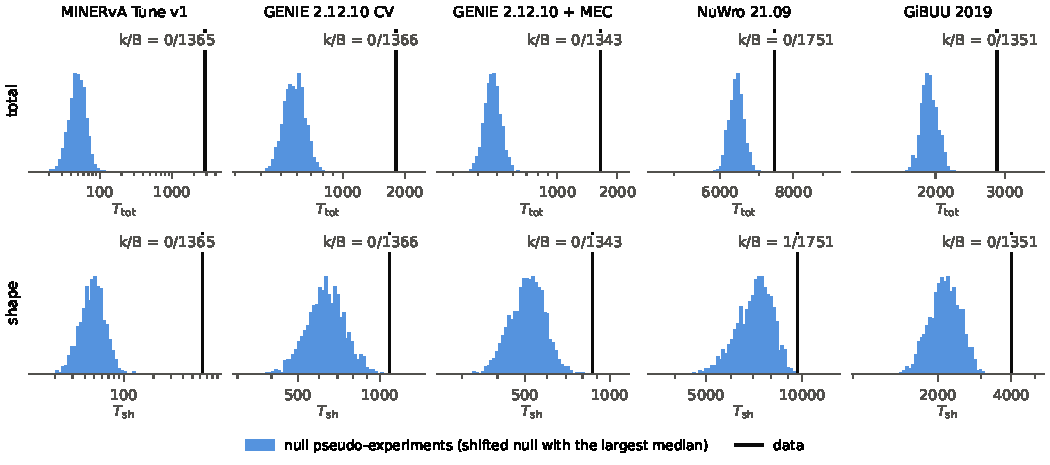
\includegraphics[width=\textwidth]{paper_joint_nulls}
  \caption{Calibrated null distributions of the joint statistics for each
  prediction (columns), total statistic (top) and shape statistic (bottom),
  shown for the declared claim variant whose null distribution has the largest
  median; the vertical line is the observed statistic and $k/B$ is as in
  Table~\ref{tab:joint5d}. The horizontal axis is logarithmic. Plotted from
  the released sufficient inputs (App.~\ref{app:release}), which reproduce
  every recorded $p$ value and decision.}
  \label{fig:joint5d-nulls}
\end{figure}

\paragraph{Sensitivity to the sub-fine-grid residual.}
\label{sec:joint5d-kappa}

The multiplier $\kappa$ scales the last measured refinement change
$\delta_{\mathrm{fine}}$: $\kappa=1$ means one such change, not one standard
deviation or a confidence level. A report-only scan along the frozen direction
$\delta_{\mathrm{fine}}$~\cite{JointTestKappa2026} found all ten decisions to
remain determinate rejections at every sampled multiplier up to 5.25 in the
frozen ensembles. Determinate rejection is first lost between the sampled
multipliers 5.2547 and 5.2563 (between 5.1688 and 5.1703 with the recovered
draws included), by the GENIE~2.12.10 + MEC shape test, whose interval then
contains its Holm threshold, and, through the Holm step-down, by the
GENIE~2.12.10 shape test; neither is then a determinate failure to reject. The
scan probes one prescribed direction; it establishes neither convergence nor a
bound on the actual below-grid residual, which remains unmeasured and
potentially material.

\paragraph{Power.}
\label{sec:joint5d-power}

Every test rejects, so power is context only (the contract attaches power to
non-rejections). At the Tune~v1 null, two of the three declared alternatives
are detected in shape with power 1.0 at the 0.005 level, and the third, a
MEC-like $(\Eavail,W)$ shape, with \jtPowPthree. At the GENIE~2.12.10 null the
shape powers at 0.005 are \jtPowPonegShape, 0.02 and 0.00. These come from the
frozen sets, each of which lost some of its 200 alternatives to time limits
(172--199 retained). Against the frozen null ensembles, the complete power sets
recovered as in \S\ref{sec:joint5d-lost} agree within 0.01; with the null recomputed on all draws, the first
GENIE~2.12.10 set moves to 0.72.

\subsection{Lost pseudo-experiments and their recovery}
\label{sec:joint5d-lost}

Scheduler time limits interrupted or prevented \jtLostCal{} of the submitted
calibration pseudo-experiments (\jtLostInterrupted{} interrupted,
\jtLostNever{} never started) and \jtLostPow{} power pseudo-experiments, so the
decisions in Table~\ref{tab:joint5d} were evaluated on the completed draws. A
sensitivity computed before the lost outcomes were known showed that every
decision could change under a realizable assignment of them: had every
interrupted draw exceeded the observed statistic, no test would have been
rejected ($p$ \jtWorstIntLo--\jtWorstIntHi). Among completed draws, runtime is
not associated with the statistic ($|\rho|\le\jtRuntimeRho$), which supports
but does not certify the decisions.

The lost seeds were therefore rerun, report-only, under a procedure fixed and
independently reviewed beforehand~\cite{JointTestRecovery2026}. A determinism
check fixed in advance (16 of 16 completed seeds rerun bitwise identically)
shows that each recovered draw is the lost draw, so every submitted draw has
now been observed. No recovered draw reaches the observed statistic in any
test, claim variant or robustness variant, so no assignment of the lost draws
changes any decision. The closest margin is 4.6 units of $T$ below the observed
value of 868.6 (GENIE~2.12.10 + MEC shape, $\pm\jtMoneKappaRobust\,\delta_{\mathrm{fine}}$
variant); the next is 49.8 (GENIE~2.12.10 shape, same variant). With complete
batches the frozen rule would have stopped the Tune~v1, GENIE~2.12.10,
GENIE~2.12.10 + MEC and GiBUU nulls one batch earlier ($B=1200$), with the same
decisions.

The scope of the recovery's checks is narrower than that of the main
recomputation:
\begin{itemize}[itemsep=1pt, topsep=2pt]
  \item its independent cross-check (856 of 856 quantities) covers only the
        reading with the frozen variant shifts;
  \item the reading with the recovered draws added to the calibration (the
        shift recomputed on all draws) was reproduced only by a standalone
        replay of the same code, a consistency check rather than an
        independent recomputation;
  \item the earlier-stop decisions rest on the campaign's self-validated
        re-application of the sequential rule.
\end{itemize}
The recovery is report-only: the primary decisions are those of the frozen
evaluation, at the frozen $B$, and the recorded disposition of the recovery
is ``certified, margin disclosed''.
% Source: RECORD-20261006-s5p-lost-seed-recovery-resolution.md (recovery, margins 4.6/49.8 T units, earlier
% stops, power over the complete sets); RECORD-20261005 sec. 5 (pre-recovery sensitivity, |rho| <= 0.06);
% DECISION-20261005-s5p-recompute-extension-and-lost-seed-recovery.md sec. 5 (Joseph's disposition).

\subsection{Matched coarse projections}
\label{sec:joint5d-projections}

Restricting the same calibrated tests to matched $3\times3$ coarse projections
of the same cells, onto $(\pT,\pPar)$ and onto $(\Eavail,W)$, gives $p<0.05$
for every test in at least one of the two projections, so this study provides
no evidence of additional discrimination from the joint five-observable
information. The comparison was specified before it was run but after the
five-dimensional outcomes were known; it uses the same calibration ensembles,
with the recovered draws included, and the same variants and claim rule, and
its $p$ values were reproduced independently~\cite{JointTestProjections2026}.
In the muon-only $(\pT,\pPar)$ projection, GENIE~2.12.10 is not rejected
($p=\woneGcvPtTot$ in total, $\woneGcvPtShape$ in shape; a post hoc
observation), whereas its $(\Eavail,W)$ projection is. Hadronic information
therefore participates in that rejection; this does not establish added power
of the joint test over all matched projections, or accept GENIE as true.

\subsection{Hadronic-response condition and recoil-energy sensitivity}
\label{sec:joint5d-response}

MINERvA's recoil-energy analyses assign a hadronic-energy response uncertainty
derived from test-beam calorimetry~\cite{MINERvA:2015testbeam}, separate from
the GEANT hadron-interaction reweights~\cite{MINERvA:2021owq,MINERvA:2022incl};
in the low-recoil measurement the resulting hadronic-energy uncertainty rises
to \SI{10}{\percent} at its highest three-momentum transfers,
$0.9<q_{3}<\SI{1.2}{GeV}$~\cite{MINERvA:2022incl}. The declared nuisance model
here includes the reweights but no calorimetric response band. Such a band
would act on all five nulls together, through the shared detector simulation
and unfolding: a response mismodelling could move each observed statistic in
either direction, and a band drawn in the calibration would also broaden and
could shift each null distribution; the net effect on each $p$ value is
unmeasured. The published comparison in muon kinematics alone, whose
observables do not use the reconstructed recoil energy, also disfavours the
same generator families~\cite{MINERvA:2021owq}; it provides context for a
disagreement involving muon observables, but the hypotheses tested here use a
different estimator and calibration. The GENIE~2.12.10 projection result of
\S\ref{sec:joint5d-projections} shows that the information rejecting that
prediction involves the hadronic axes, on which a response band would act.

For an exploratory response sensitivity study~\cite{JointTestRecoil2026}, the
data are re-unfolded with the simulation's reconstructed recoil energy scaled
by $\pm\SI{4}{\percent}$, and the frozen tests are re-evaluated against the
frozen null distributions. The size is the level of data--simulation agreement
reported for test-beam protons, pions and electrons of
0.35--\SI{2.0}{GeV/c}~\cite{MINERvA:2015testbeam}; neutrons and
higher-momentum hadrons, which matter at high $W$, lie outside that sample.
The $\pm4\%$ size is a labelled exploratory sensitivity, not a validated
uncertainty prescription. A re-unfold with unscaled recoil reproduces
the frozen decisions, with every claim $p$ value inside the range spanned by
the data's rounding variations. At both $-4\%$ and $+4\%$ every one of the ten
rejections holds. The observed statistics move by up to about \SI{11}{\percent}
from their frozen values, nine tests keep $k=0$, and NuWro's shape test, the
closest to its null, changes from $k=1$ to $k=3$ of 1751 at $+4\%$
($p=0.0023$, against a Holm threshold of 0.05). The evaluation was reproduced
independently.

The calibration distributions stay fixed in this study, which measures the
sensitivity of the observed statistics and decisions to one coherent scale of
reconstructed available energy and recoil energy, applied after the energy
calibration at a single magnitude. A response-uncertainty construction would
also need to vary the null distributions. The study leaves untested (a) the
response of the null distributions, which were not regenerated with the
variation although they are simulated through the same detector model, so the
size of this omission is unmeasured for these strongly non-central nulls;
(b) particle-species, energy-dependent or resolution effects, and a response
difference applied before calibration; and (c) larger variations. The
rejections are therefore conditional on the simulation's hadronic response,
and the response model is not shown to be complete.

\subsection{What the tests establish}
\label{sec:joint5d-reading}

The comparisons recover the generator disagreements already established by
the published two-dimensional measurement on the same
data~\cite{MINERvA:2021owq}. Their methodological contribution is calibration
through the full analysis chain, which puts the estimator's bias toward its
prior and the declared nuisances into each null distribution. The rejections
are global assessments of the five specified predictions under the declared
model; assigning a discrepancy to a kinematic region or nuclear mechanism
would require separate tests. They apply to the generator versions listed in
\S\ref{sec:eavailw-band} and retain all six conditions of
\S\ref{sec:joint5d-conditions}; in particular, the hadronic response and the
sub-fine-grid residual remain outside any validated uncertainty bound.
Extending the inference would require a response band drawn through the
calibration and a demonstrated bound on the residual below the fine grid.
% Source: docs/orchestration/RECORD-20261005-s5p-joint-5d-inference-result.md (decisions, B, k, p, the six
% conditions); DELIVERY-20261006-s5p-campaign-terminal.md; W1 (docs/publication/w1/W1-RECORD-20261006.md);
% W2 (publication/w2/W2B-REPORT-20261006.md); kappa (publication/kappa/RECORD-20261008-kappa-breakdown.md).
% Section assembled 2026-10-11 from the article's former Sec. VI and the note's former sec_eavailw subsection,
% when the article's joint-test section was shortened.

\section{Extended fiducial phase-space study}
\label{sec:fps}

This section gives a preliminary scalar central value for an extended fiducial domain, with a three-prior
dependence envelope, a hidden-variable closure and a 200-toy containment diagnostic for the extension. The
signal remains $\nu_\mu$ CC in the tracker interaction fiducial volume. The truth-muon
kinematic cuts are removed, but the reconstructed MINOS-based selection is unchanged,
so the domain is an extended \emph{fiducial} one, not unrestricted neutrino phase space. No covariance is
quoted for it, so the result consists of central values and these validation tests.
% Accuracy fix (unscored; Joseph, DECISION-20261026-joseph-fps-scope-r04-sensitivity-and-tex-reflow.md, via the director 2026-10-26): "No corrected covariance exists for it" was
% false as read: an extended-fiducial covariance with re-selected lateral bands exists (job 56431823, 2026-08-07;
% nd-unfolding/uq_fps/corrected/FPS_UQ_CORRECTED_STATE.md:127) but is not quoted (AGENTS.md:36).
% Search: extended-fiducial covariance quoted; corrected FPS covariance; activelat (note, paper and primer closures: no
% printed extended-fiducial covariance or uncertainty beyond the three-prior envelope; AGENTS.md:36 "Old unified 4D/FPS
% covariances ... are unquotable") @ 7ad668f4
% Register pass b8 (2026-10-22): register only; every number and limitation kept (ledger.md rows F*).

\subsection{Acceptance and the extended domain}
The published cuts ($\theta_\mu<20^{\circ}$, $1.5<\pPar<\SI{60}{GeV/c}$,
$\pT<\SI{4.5}{GeV/c}$) exclude a third of the signal. Of the weighted true
$\nu_\mu$~CC rate in the tracker fiducial volume, \SI{66.4}{\percent} lies
inside the cuts, \SI{22.3}{\percent} at $\pPar<\SI{1.5}{GeV/c}$,
\SI{11.3}{\percent} at $\theta_\mu>20^{\circ}$, and the high-$\pT$/$\pPar$
tails are negligible (Fig.~\ref{fig:fpsacc}). OmniFold's treatment of events that fail reconstruction
already corrects for acceptance, so removing the truth-level kinematic cuts is a change of configuration
only: the truth denominator grows from 32.8 million to 49 million events, and the reconstruction
selection, including the MINOS match, is unchanged. In regions without acceptance the unfold extrapolates
through the step-1 regressor for missed events; the validation tests below quantify the resulting
prior dependence.

\begin{figure}[H]
  \centering
  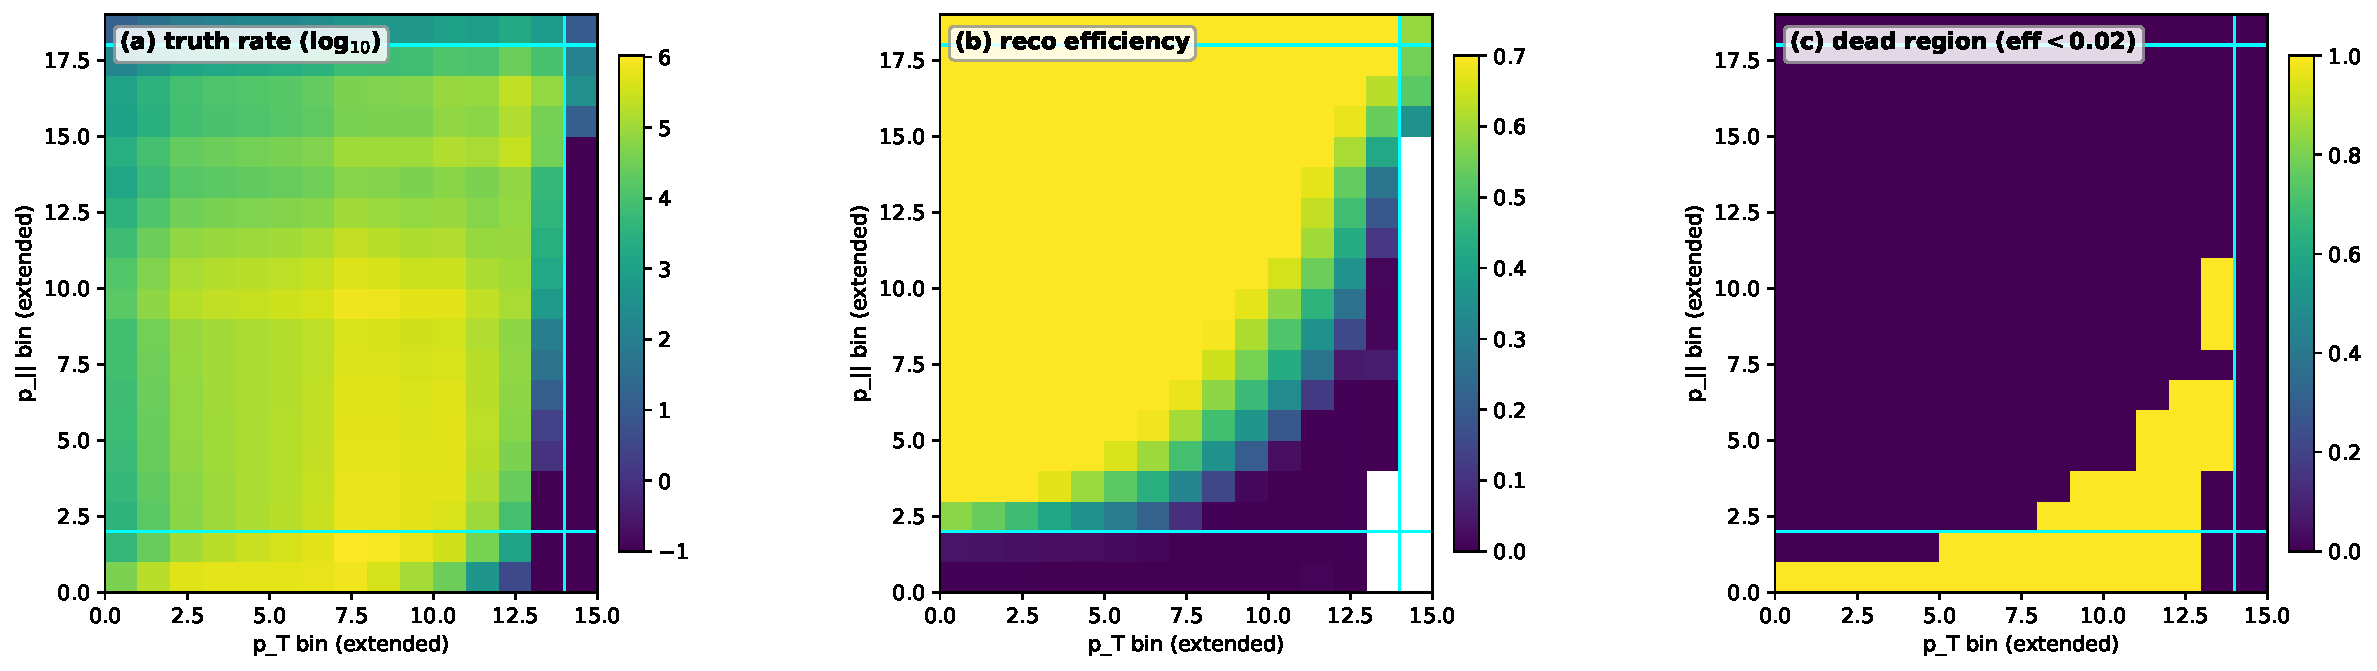
\includegraphics[width=0.99\textwidth]{fps_acceptance_MEFHC}
  \caption{Extended-fiducial acceptance across all twelve playlists:
  (a)~weighted truth rate (log$_{10}$), (b)~reconstruction efficiency, and
  (c)~the dead region with $\epsilon<\SI{2}{\percent}$, on the extended
  $(\pT,\pPar)$ grid (bin number; catch bins are too wide for a linear
  axis). Cyan lines mark the published boundary. Efficiency is
  $\sim0.65$ and flat through the published region, degrades smoothly across
  the $\theta>20^{\circ}$ wedge, and falls to zero in the $\pPar<\SI{1.5}{GeV/c}$
  strip and the high-$\pT$ corner. The dead region carries
  \SI{27.7}{\percent} of the total truth rate.}
  \label{fig:fpsacc}
\end{figure}

\subsection{Validation battery}
Four tests characterize the extension (Fig.~\ref{fig:fpscmp}):
\begin{enumerate}[itemsep=2pt]
  \item \textbf{Published-region check.} In the published sub-block, the extended unfold reproduces the control
        (standard 2D input, paper grid, identical settings) with
        integral ratio $0.9994$, median cell ratio $1.0013$, and median
        deviation \SI{\fpsAnchor}{\percent} across all 185 reported cells:
        in the published region the extended unfold agrees with the control at this level. The control's
        total, $\SI{\sigTwoDPurity}{cm^2/nucleon}$, equals at the printed precision that of the
        purity-subtracted 2D central values (exact-split and LightGBM). The quoted 2D result, with refined
        negative-weight subtraction, is $\SI{\sigTwoD}{cm^2/nucleon}$, \SI{\roFpsDiff}{\percent} lower, so the
        control no longer reproduces it.
% RE-2 integration W3 (approved, DECISION-20261024-joseph-approve-integration-wording-s1-compute-preserve.md): RE2-PARTC-REPORT.md sec. 8 (RO-FPS: E_R 3.069e-38 against the control's 3.073e-38, -0.14 %,
% "It does not reproduce"); the control: VALIDATION_LEDGER.md:1624-1625 (no committed digest; VL177 records the -0.14 %); the exact-split total
% 3.0733e-38 (values.tex \sigTwoD comment).
  \item \textbf{Closure.} Extended-grid self-closure using simulated reconstruction as
        pseudo-data returns recovered/truth $=1.0000$ in every cell,
        including the extension, with no event-accounting or normalization bias
        from the enlarged denominator. In \emph{hidden-variable} closure,
        a Gaussian truth bump is injected in true $E_{\mathrm{avail}}$,
        unseen by the $(\pT,\pPar)$ unfold. The recovered cross section
        reproduces the bump-reweighted $(\pT,\pPar)$ truth to
        median \SI{0.17}{\percent} (90th percentile \SI{0.65}{\percent}) in
        the published cells and median \SI{0.77}{\percent} (max
        \SI{4.05}{\percent}) in the extension, both well inside the prior envelope.
  \item \textbf{Three-prior envelope.} Repeating the unfold with three priors
        (MINERvA Tune~v1, bare GENIE, and NuWro-shaped) spans the
        total cross section by only $\pm\SI{1.5}{\percent}$. The NuWro-shaped
        prior reweights the truth $(\pT,\pPar)$ shape to two million raw
        NuWro events without phase-space cuts. The sample's mis-sampled flux
        (\S\ref{sec:3d-models})
        % \texttt{KNOWN\_ISSUES.md} row 83; flux repair of 2026-09-27
        suppresses its high-$\pPar$ shape, and this prior was not rebuilt after
        the flux repair. Per-cell half-spread/mean has median
        \SI{2.9}{\percent} in the published region and \SI{7.9}{\percent}
        (90th percentile \SI{62}{\percent}) in the extension, concentrated
        in zero-acceptance cells (Fig.~\ref{fig:fpsenv}).
  \item \textbf{Containment diagnostic.} With a fixed estimator seed and one 100/100 calibration--evaluation
        split, widths learned from the disjoint calibration half contain the
        fixed truth in \SI{\covFPS}{\percent} of evaluation bin--toy cells,
        compared with the \SI{\covNominal}{\percent} Gaussian nominal.
        Bin correlations and estimated widths preclude a global binomial error
        or a calibrated test. The diagnostic probes the statistical closure-toy stream, not a full uncertainty band.
        The statistical-band, pull and regional fractions are in App.~\ref{sec:fps-fractions};
        none is used as a covariance-certification test.
\end{enumerate}

\begin{figure}[H]
  \centering
  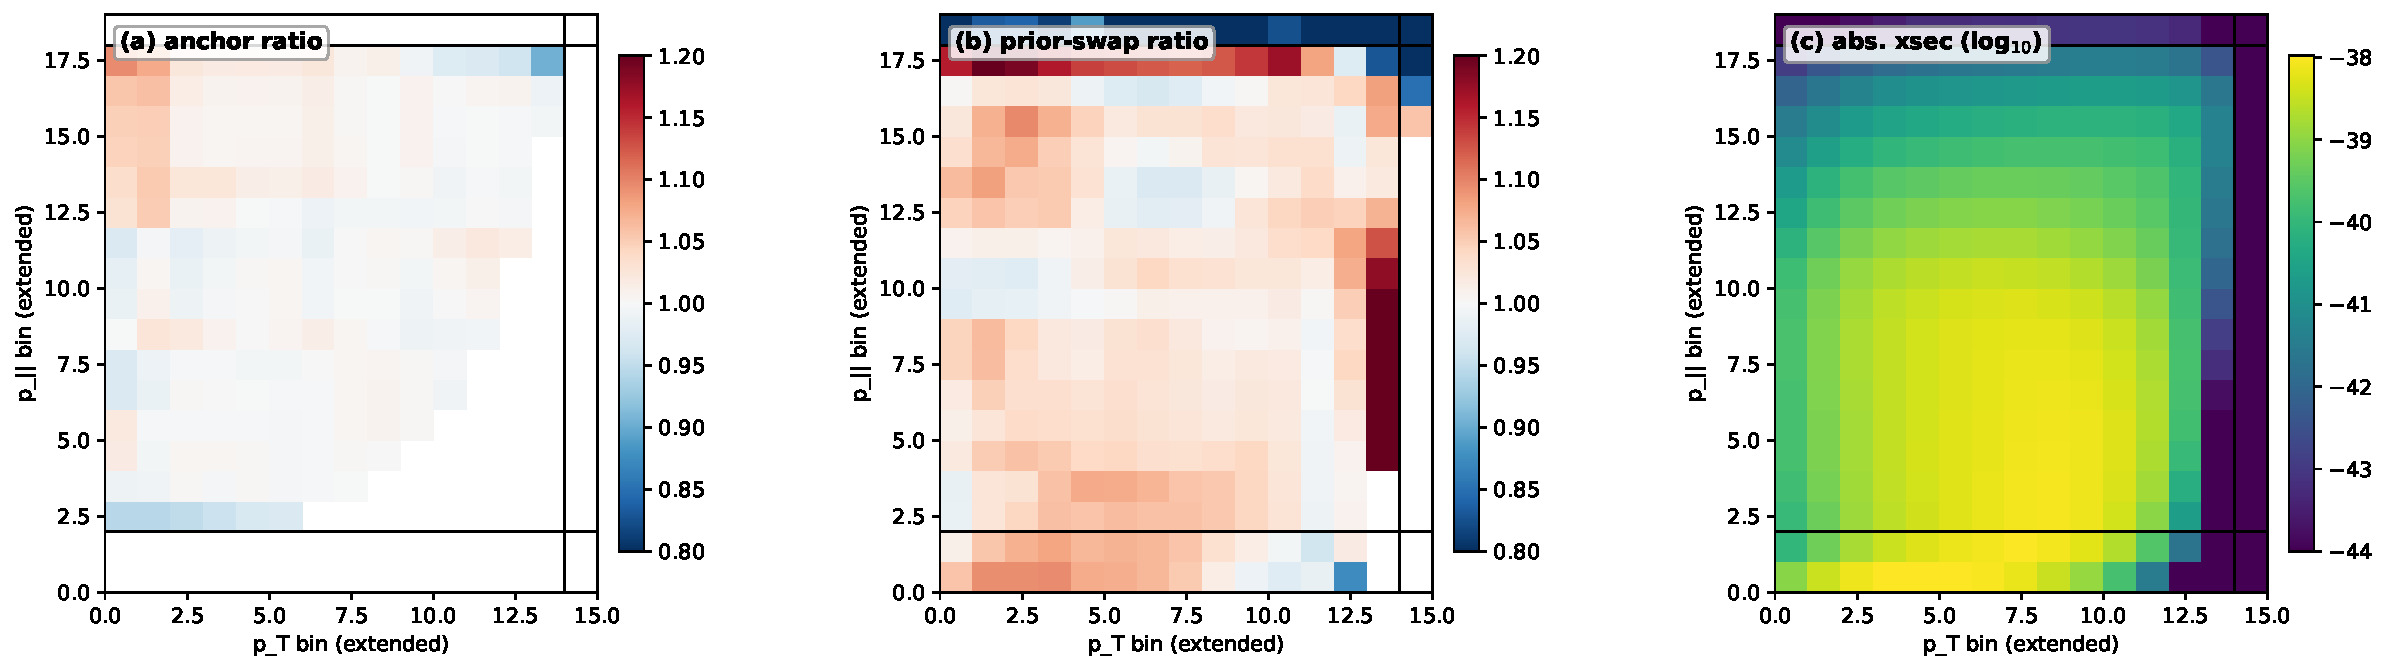
\includegraphics[width=0.99\textwidth]{fps_pilot_compare_MEFHC}
  \caption{Extended-fiducial validation battery (all playlists):
  (a)~ratio to the control in the published sub-block (median $1.0013$), (b)~MINERvA Tune~v1/bare-GENIE prior-swap ratio, and (c)~extended-fiducial
  cross section (log$_{10}$). Panels (a) and (b) are \emph{ratios} (diverging
  scale centered at unity); (c) gives \emph{absolute} magnitude on a sequential
  scale --- hence the two color schemes. Black lines mark the published
  boundary; axes are bin number on the extended grid.}
  \label{fig:fpscmp}
\end{figure}

\begin{figure}[H]
  \centering
  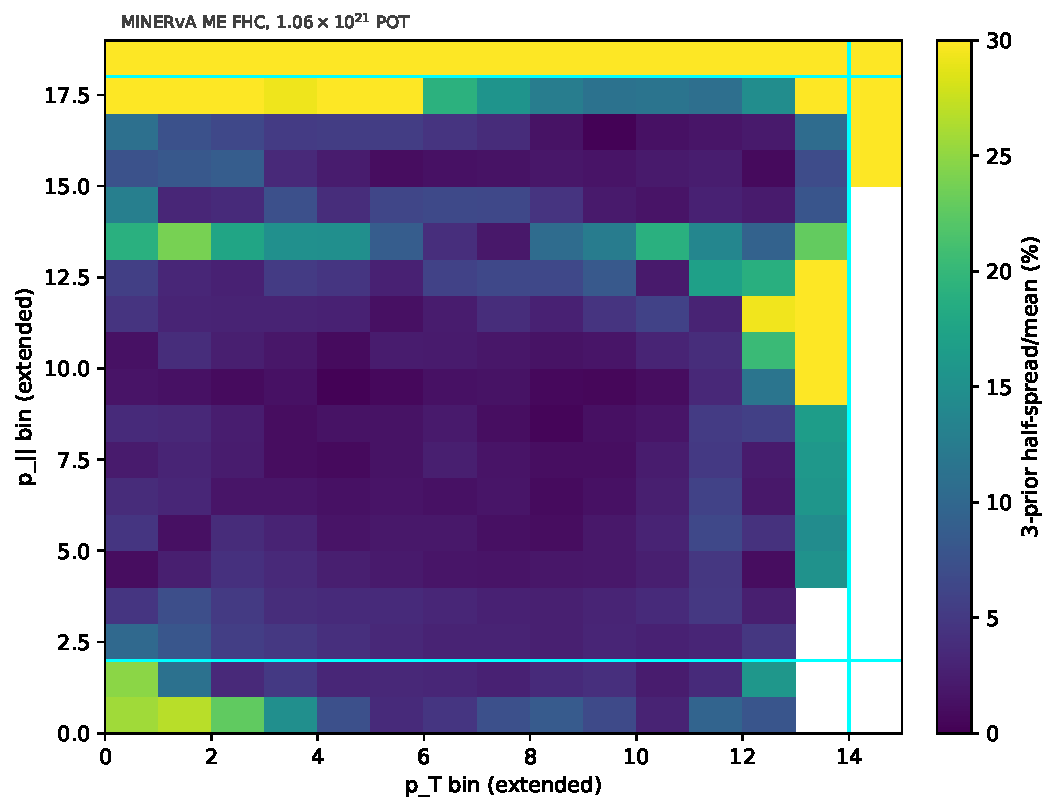
\includegraphics[width=0.62\textwidth]{fps_prior_envelope_MEFHC}
  \caption{Three-prior dependence envelope (half-spread/mean per cell,
  in percent). Prior dependence is at the few-percent level wherever the
  detector has acceptance and reaches tens of percent only in the dead
  cells --- the quantitative basis for the two-tier reporting.}
  \label{fig:fpsenv}
\end{figure}

\subsection{Central value and two-tier reporting}
The preliminary extended-fiducial CC-inclusive central value on the tracker
fiducial volume is
\begin{equation*}
  \sigma_{\mathrm{ext}} = \SI{\fpsSigma}{cm^2/nucleon}
  \quad\text{(central value)},
\end{equation*}
% RE-2 integration W5 (approved, DECISION-20261024-joseph-approve-integration-wording-s1-compute-preserve.md): \fpsAbove (46) is not printed; its definition is not established (RE2-PARTC-REPORT.md
% sec. 4: 4.502/3.0730 - 1 = 46.50 %; VALIDATION_LEDGER.md:1626 "+46% vs restricted" names no operand). The two totals:
% VALIDATION_LEDGER.md:1624-1625 (control 3.073e-38; FPS total 4.502e-38).
compared with $\SI{\sigTwoDPurity}{cm^2/nucleon}$ for the control unfold in the restricted phase
space. The extended-fiducial central value was produced with the binned purity correction (the battery of 2026-06-10), not
with refined negative-weight subtraction, the treatment designated for the extended-fiducial analysis (App.~\ref{app:negweight}).
% Accuracy fix (unscored; Joseph, DECISION-20261026-joseph-fps-scope-r04-sensitivity-and-tex-reflow.md, via the director 2026-10-26): "No extended-fiducial production with
% refined negative-weight subtraction has been run" was false as read: ten negweight-refined extended-fiducial endpoint
% unfolds were run later (job 56430128; nd-unfolding/sbatch_unfold_active_fps.sh:18,34-35,60). The sentence now says
% only what the quoted central value used, in the words of Joseph's selected option, and keeps the base sentence's fact that a
% negative-weight treatment is designated for this analysis. That treatment is refined negative-weight subtraction: App. C
% sec:negweight-footing designates negative-weight injection with Stay-Positive refinement (app_negweight.tex:370-371), the
% refined form of negative-weight injection (:257-258) whose refinement is the Stay-Positive classifier (:476) (director, 2026-10-26).
% Search: extended-fiducial central value; fps battery; 54244120; negweight-refined FPS central value (app_provenance.tex
% fps-battery; no refined extended-fiducial central value is recorded; sbatch_unfold_active_fps.sh:67 takes the existing
% central value as input) @ 7ad668f4
We adopt \textbf{two-tier reporting}.
\emph{Tier~1} comprises the acceptance-supported cells ($\epsilon\gtrsim2\%$): the published region and the
measurable part of the extension, which carries $\sim\SI{6}{\percent}$
of the rate, chiefly in the $\theta>20^{\circ}$ wedge and the
$\pPar\in[0.75,1.5]\,\si{GeV/c}$ edge. \emph{Tier~2}, prior-extrapolated,
comprises the dead cells ($\sim\SI{28}{\percent}$ of the rate) and is flagged separately with
an explicit additional three-prior envelope band. Both tiers enter the
sum; only tier~1 is interpreted as an acceptance-supported measurement.
No uncertainty magnitude is assigned beyond the three-prior envelope, because no extended-domain
covariance has been constructed with re-selected lateral bands under the procedure of \S\ref{sec:uq-combine}.
% Search: extended-domain covariance with re-selected lateral bands; activelat; 56431823; sec:uq-combine procedure (true as scoped, Joseph's ruling DECISION-20261026-joseph-fps-scope-r04-sensitivity-and-tex-reflow.md item 1.3: the activelat FPS covariance of job 56431823, AUDIT-FINDINGS-20260820-fps.md:217-221, was built on 2026-08-07, before the sec:uq-combine procedure with C_PL was adopted on 2026-10-17, DECISION-20261017-joseph-2d-adopt-s5-plus-playlist.md, and is unquotable, AGENTS.md:36, AUDIT-FINDINGS-20260820-fps.md:389-390) @ 0d9c64fd
% The former subsection "Recoil-PET feasibility study on the extended population"
% (label sec:fps-pet) moved to sec_pet.tex, sec:pet-full-event-status (lane 3 §10.1).

\section{Summary and outlook}
\label{sec:summary}

\paragraph{Summary.}
The executive summary (\S\ref{sec:execsummary}) lists each result with its
scope; this section states the conclusions they support.
\begin{itemize}[itemsep=2pt]
  \item Unbinned OmniFold with gradient-boosted trees reproduces the published
        MINERvA ME FHC CC-inclusive $d^{2}\sigma/(d\pT\,d\pPar)$ and its
        uncertainty scale (\S\ref{sec:results}), with a correlated shape
        difference along the low-$\pT$ peak ridge
        ($\chi^{2}/\mathrm{ndf}=\chiPaper$, \S\ref{sec:results-tension}). The
        uncertainty is computed with LightGBM ensembles and its transfer to the
        exact-split central value is unmeasured (\S\ref{sec:method-config}); the
        first-built statistical band failed a fixed-truth coverage test in its
        tails and the rebuilt band has not been re-tested (\S\ref{sec:coverage}).
  \item Simultaneous unbinned three-, four- and five-observable unfolds
        ($+\Eavail$, $+q_{3}$, $+W$) agree with their lower-dimensional
        predecessors to $\approx$1--2\,\% and recover an injected $\Eavail$
        shape (\S\ref{sec:3d}). They recover the established low-recoil 2p2h
        deficit (\S\ref{sec:3d-2p2h}), resolve its momentum-transfer structure
        (\S\ref{sec:4d}), and place the remaining high-$\Eavail$ excess over the
        Tune~v1 prior in the deep-inelastic region, where all four external
        generators lie below the data, each by about its overall shortfall after
        accounting for the $E_\nu>\SI{20}{GeV}$ events missing from GiBUU
        (\S\ref{sec:eavailw-band}).
  \item The five-axis estimator does not follow generator-sized truth changes,
        and its measured model dependence rules out every predeclared
        five-dimensional reporting definition at useful precision; no
        five-dimensional interval coverage is established (\S\ref{sec:5d}). The
        one adopted five-axis covariance carries estimator-seed sensitivity
        above its declared limit, so no covariance-based significance is quoted
        (\S\ref{sec:eavailw-adopted}).
  \item Calibrated through the full analysis chain, frozen joint tests reject
        all ten simple generator hypotheses under six stated conditions. They
        recover established discrepancies, show no discrimination beyond matched
        coarse projections, and add no reportable uncertainty
        (\S\ref{sec:joint5d}).
  \item The point-cloud (PET) track is diagnostic and method development, with
        no adopted covariance and no eligible full-event design
        (\S\ref{sec:pet}, \S\ref{sec:pet-campaigns}).
\end{itemize}
% 2026-10-11: shortened. The earlier bullets restated the executive summary item by item; the original text
% (with its lane-review cut comments) is in git history at e25abfd5:docs/analysis-note/sec_summary.tex.

\paragraph{Outlook.}
The scalar extended-fiducial study (\S\ref{sec:fps}) yields a preliminary
central value $\sigma_{\mathrm{ext}}=\SI{\fpsSigma}{cm^2/nucleon}$
(\SI{\fpsAbove}{\percent} above the restricted phase space).
% Cut (lane 3 §11 #8; stated at the head of sec_fps.tex): with an anchor,
% closure tests and a three-prior envelope but without a corrected covariance
New acceptance-supported cells contribute about \SI{6}{\percent} of the rate;
separately labeled prior-dominated extrapolation contributes about
\SI{28}{\percent}. The full-event PET candidate
(\S\ref{sec:pet-full-event-status}) remains method development, off the
publication critical path.
% Cut (lane 3 §11 #5, lane 5 R8; stated in sec_pet.tex): The full-event PET candidate adds the
% distinguished muon and declared event context; nominal and unverified
% $C_{\rm stat}$ artifacts exist, but their pairing was declined and no PET
% covariance is adopted. Its remaining closure and complete-UQ requirements are
% method development and are not on the publication critical path.
The publication critical path ran through the adoption of a selection-complete
scalar five-dimensional covariance, which has happened under exception
(\S\ref{sec:eavailw-adopted}) and never through PET; the precision-measurement
objective is not complete, because the five-dimensional measurement branch was not
admitted (\S\ref{sec:gbdt-model-dependence}).
% Resolves the demoted TODO (lane 5 R12) on the scalar-5D campaign (s5p, OI-193) closing.
% Source: docs/orchestration/RECORD-20261005-s5p-joint-5d-inference-result.md section 7 (NOT ADMITTED,
% no new reportable uncertainty, NOT READY); CHECKLIST-20261001-s5p-terminal-and-claims.md section 4.
Further refinements are a fifth generator, NEUT, and a finer 44-cell Ascencio
comparison (maximal-common-grid comparison in \S\ref{sec:4d}).
A paper-independent flux\,$\leftrightarrow$\,muon posterior from MAT-MINERvA
for a fully self-derived $\rho$ would further strengthen the analysis.
% Withdrawn outlook item moved to App. H (sidecar appH-additions.tex, "From \S\ref{sec:summary}, outlook"):
% The truncated-spectral ``ours-only'' goodness-of-fit convention
% (App.~\ref{sec:rank}) is no longer among them: the collaboration confirmed it
% uses the same truncated-spectral pseudo-inverse.

\paragraph{Reusing the unbinned result.}
The public ATLAS charged-particle phase-space release
\cite{ATLAS:2026fpsdata} exemplifies unbinned distribution. The emerging
\texttt{omnifold\_publication} proposal \cite{Bajpai:2026publication} emphasizes
weight-family metadata, normalization, row alignment, and checksums.
A MINERvA release should likewise specify event
identity, estimator and uncertainty-family definitions, units, support,
normalization, and a reproducible projection example.
App.~\ref{app:release} specifies this release for our analysis. It records
which objects have fixed identities today and which do not exist yet.
\textbf{No release tag or release manifest
exists}; rebuilding the documents reproduces no result here. New projections
require their own applicability checks; nominal weights alone cannot certify arbitrary
downstream inference (App.~\ref{sec:unbinned-inference}). The release design and
public example have no bearing on the separately settled covariance adoption
(\S\ref{sec:eavailw-adopted}).


\section*{Acknowledgments}
This
analysis was carried out on the Perlmutter system at the National Energy
Research Scientific Computing Center (NERSC), a U.S.\ Department of Energy
Office of Science User Facility, under project m3246. It builds on the MINERvA
Analysis Toolkit (MAT) and the MINERvA-101 cross-section framework, and we thank
their authors. We are grateful to the MINERvA Collaboration for the public release
of the medium-energy CC-inclusive data product on which the reproduction rests.

We thank Callum Wilkinson for connecting us with this dataset and for many helpful discussions.
We thank Kevin McFarland for suggesting a detector-response-mismatch closure
targeting correlations among the reconstructed hadronic observables.

% Aligned with the article's statement (main_paper.tex acknowledgments), 2026-10-11.
The analysis code, statistical procedures, computing campaigns, independent
recomputations and reviews, figures, and manuscript drafts were produced with
substantial assistance from AI language-model tools, used through the Claude
Code and OpenAI Codex command-line agents: Anthropic Claude (Opus 4.7, 4.8, 5,
and 5.5; Fable 5 and 5.1) and OpenAI GPT models (GPT-5.5, GPT-5.6 Sol and Luna,
GPT-6 Astra, and GPT-6.1), including those used for independent review. The
authors directed this work through written specifications fixed before each
study. Results were accepted only after verification against committed
evidence: predeclared criteria, independent recomputation by separately written
code (for example, the joint-test evaluation and the lost-seed recovery), and
independent read-only reviews. AI tools were also used for methodological
discussion. The figures were drawn by plotting code
from the analysis outputs; no image was generated or edited by a generative-AI
image tool. AI tools are not authors. The authors take responsibility for the
content.

\appendix
% Guide to the appendices (note reorganization, 2026-10-11). Keep it in step with main_note.tex's
% \input order after \appendix.
\section*{Guide to the appendices}
\addcontentsline{toc}{section}{Guide to the appendices}

The appendices fall into three groups. The first gives methods and context for the body: statistical methods and the 2D comparison (App.~\ref{app:statmethods}) and those for the multidimensional results and inference (App.~\ref{app:statmethods-nd}); unbinned background subtraction (App.~\ref{app:negweight}); the protocol for a detector-response-mismatch closure, which rescales the reconstructed available energy of the pseudo-data while OmniFold keeps its nominal response (App.~\ref{app:response-mismatch}); and the survey of MINERvA measurement dimensionality (App.~\ref{app:landscape}). The second, on future work, covers point-cloud (PET) representations (App.~\ref{sec:pet}). The third describes the result package and what it reproduces (App.~\ref{app:release}) and the code layout (App.~\ref{app:codebase}); it is reference material and is not needed to follow the physics results. The provenance of the records the note cites, the fixed identities and audit record of the five-axis covariance of the configuration-(a) central value, the test-suite discipline, and superseded values and withdrawn results are kept in the analysis repository's records document, Ref.~\cite{NoteRecords2026}; each citation names the entry's number or heading.

\paragraph{Labels used in the repository.} The body describes each object in words: the learner backends (\S\ref{sec:method-config}), the background-subtraction modes (\S\ref{sec:method-algo}, App.~\ref{app:negweight}), the two centerings of the five-axis covariance (\S\ref{sec:eavailw-construction}), the re-selected universes (\S\ref{sec:uq-higherdim}) and the two universe sweeps (\S\ref{sec:uq-2d-construction}). Where a repository label is needed to find the object, it is given once in parentheses at first use. The learner backends are labelled \texttt{lgbm}, \texttt{exact} and \texttt{hist}: LightGBM (the quoted central values and their uncertainty ensembles; also the joint-test estimator), the scikit-learn exact-split estimator (the exact-split cross-check) and the scikit-learn histogram estimator (\S\ref{sec:method-config}). Products described as flux-corrected are those repaired for an audit finding that the $N$-dimensional code divided every flux universe by the central-value flux (App.~\ref{app:negweight}). The calls behind Eq.~\eqref{eq:bootcov}, \S\ref{app:poisson} and \S\ref{sec:invert} (default cutoff) are \texttt{np.cov(Xrep, rowvar=False, ddof=1)}, \texttt{np.random.\allowbreak default\_rng().\allowbreak poisson(1.0)} and \texttt{np.linalg.pinv}; the earlier MAT check without the normalization band (\S\ref{sec:minerva}) used the option \texttt{-{}-add-norm 0}.

\section{Statistical methods}
\label{app:statmethods}
\label{app:methods}

This appendix collects the measurement's statistical methods. These include covariance inversion, MAT-conformant construction, estimator combinations, and conventions for $\chi^{2}$, pulls, and shape-only comparisons. We discuss training-seed, bootstrap, and universe estimators, covering the Poisson limit and $\pm1\sigma$ pair covariance. The text details ill-conditioning/rank analysis, N-D rank and ndf declarations, scalar-5D diagnostic reductions, extended-fiducial band and pull fractions, and tension anatomy. Remaining topics are closure tests, the 2D audit trail and unfolded-event inference; the full-event $C_{\rm stat}$ construction has its own appendix (App.~\ref{app:cstatlimit}). The 2D fixed-truth coverage test is in \S\ref{sec:coverage} and the same-ensemble pull diagnostic in \S\ref{sec:val-other}. We focus entirely on analysis-specific conventions rather than a general statistics primer. The $\chi^{2}$ convention referenced throughout is Eq.~\eqref{eq:chi2} in \S\ref{sec:chisq}.

\subsection{Numerical conventions: inverting a covariance (Cholesky, ridge jitter, pseudo-inverse)}
\label{sec:invert}

Equation~\eqref{eq:chi2} requires inverting $\mathbf{C}$.

\paragraph{Cholesky and ridge jitter.}
$\mathbf{C}$ is positive-definite (PD) iff its Cholesky factorization
$\mathbf{C}=\mathbf{L}\mathbf{L}\T$ exists with lower-triangular $\mathbf{L}$;
then Eq.~\eqref{eq:chi2} is well-posed. Numerical noise that leaves a PD
matrix barely non-PD is repaired with an isotropic ridge $\varepsilon\,\mathbf{I}$,
% set in \texttt{uq/analyze\_uq.py}
set to
\begin{equation}
\varepsilon \;=\; 10^{-12} \,\frac{\Tr\mathbf{C}}{n},
\end{equation}
twelve orders below the mean diagonal, far below any real signal in
$\mathbf{C}$ and safely above floating-point round-off.

\paragraph{Rank deficiency at $N \le n$.}
A sample covariance from $N\le n$ replicas in $n$ bins has rank at most $N-1$
(the superseded Stage-1 bootstrap, App.~\ref{app:history}).
The Stage-2 bootstrap ($N=300 > 205$) is full-rank. Systematic rank
limitations persist at any universe count (\S\ref{sec:rank}).

\paragraph{Pseudo-inverse.}
For the $\chi^{2}$ against the paper covariance,
% (\texttt{compare\_to\_paper\_fullcov.py})
the comparison replaces $\mathbf{C}^{-1}$
with the Moore--Penrose pseudo-inverse computed via SVD,
$\mathbf{C}=\mathbf{U}\Sigma\mathbf{V}\T$ with
$\Sigma=\diag(\sigma_{1},\dots,\sigma_{n})$:
\begin{equation}
\mathbf{C}^{+} \;=\; \mathbf{V}\,\Sigma^{+}\,\mathbf{U}\T,
\qquad
\Sigma^{+}_{ii} \;=\;
\begin{cases}
1/\sigma_{i} & \sigma_{i} > \tau,\\
0 & \text{otherwise}.
\end{cases}
\end{equation}
It calls \texttt{np.linalg.pinv} with no \texttt{rcond} argument,
% (lines \texttt{103} and \texttt{124})
so it uses NumPy's documented default cutoff,
$\tau = \texttt{rcond}\cdot\sigma_{\max}$ with $\texttt{rcond}=10^{-15}$.
The $n\,\sigma_{\max}\varepsilon_{\text{machine}}$ convention belongs to
\texttt{np.linalg.lstsq} and MATLAB (App.~\ref{app:history}).
Modes below the cutoff receive inverse weight $0$ rather than $\infty$,
keeping the quadratic form stable for zero or near-zero eigenvalues.

\subsection{Variance-source procedures}
\label{sec:variance}

Table~\ref{tab:variance-sources} summarizes the three variance sources, their
MAT reference and combination. Definitions and otherwise unreported values
follow; \S\ref{sec:systematics} describes the measurement's block construction,
and Table~\ref{tab:uq} gives the 2D budget.

\begin{table}[!htbp]
\centering\footnotesize
\setlength{\tabcolsep}{3pt}
\begin{tabular}{@{}>{\raggedright\arraybackslash}p{0.12\textwidth}
                >{\raggedright\arraybackslash}p{0.17\textwidth}
                >{\raggedright\arraybackslash}p{0.39\textwidth}
                >{\raggedright\arraybackslash}p{0.1\textwidth}
                >{\raggedright\arraybackslash}p{0.13\textwidth}@{}}
\toprule
Source & What it estimates & Procedure & Ensemble & Value / where reported \\
\midrule
Training-seed variation (ML) & Variance from random choices inside the GBDT optimizer at fixed inputs (the ``ML noise floor'') &
  Full $5$-iteration MEFHC \texttt{lgbm} unfolds (the backend of the bootstrap and universe ensembles, not of the exact-split central value), varying only the GBDT \texttt{random\_state}; seeds $(N,N{+}1,N{+}2)$ for (step-1 classifier, step-2 classifier, miss regressor), $N \in \{1,\dots,10\}$ &
  $n=10$ &
  median $0.166\%$; Table~\ref{tab:combine} \\
Poisson bootstrap (stat) & Data- and MC-statistical variance, propagated coherently through the full pipeline &
  Per-event Poisson(1) factors from independent data (seeded from $k$) and MC (seeded from $k + 10^{7}$) sub-RNGs; one MC factor on both reco and truth copies of each event; $5$-iteration re-unfold with the GBDT seed pinned &
  $N=300$ (Stage-1: $N=50$) &
  median $0.674\%$; Table~\ref{tab:combine} \\
Universes (syst) & Flux, detector and interaction-model uncertainty, by re-unfolding under reweighted MC &
  The event loop dumps truth and reco weights per (band $B$, universe $u$); each $(B,u)$ is re-unfolded with a fixed seed against a matched CV job (same omnifile, backend, seed, iteration count and flux, so ML noise cancels); MAT per-band covariance, Eq.~\eqref{eq:matcov}, plus a rank-1 normalization &
  $187$ universes, $44$ bands, $+$ norm &
  median $6.830\%$; Table~\ref{tab:band-medians} \\
MAT reference & How MINERvA builds its published covariance &
  Read from the MAT source (\texttt{MnvVertErrorBand::\allowbreak CalcCovMx}, \texttt{MnvH1D::\allowbreak GetTotalErrorMatrix}); our rollup compared with it element by element &
  $44$ bands / $187$ universes &
  max.\ rel.\ difference $5.5\times10^{-17}$ \\
Block sum & Total uncertainty covariance &
  Element-wise sum of the three independent blocks, Eq.~\eqref{eq:blocksum} &
  --- &
  median $6.871\%$; Table~\ref{tab:combine} \\
\bottomrule
\end{tabular}
\caption{Variance-source procedures for the 2D measurement ($205$ reported bins).
Code pointers: App.~\ref{app:provenance} (\texttt{variance-sources}).}
\label{tab:variance-sources}
\end{table}

\subsubsection{Training-seed variation}
\label{sec:seedscan}
For each reported bin $i$, \texttt{seedscan} uses the $n$ trials
$X_{i}^{(1)},\dots,X_{i}^{(n)}$ to estimate the unbiased sample standard deviation
\begin{equation}
\sigma^{\ML}_{i}
\;=\;
\sqrt{\frac{1}{n-1}\sum_{k=1}^{n}\big(X^{(k)}_{i}-\bar X_{i}\big)^{2}},
\qquad
\bar X_{i} = \frac{1}{n}\sum_{k} X^{(k)}_{i},
\end{equation}
and reports the median $\sigma^{\ML}_{i}/\bar X_{i}$ over $205$ bins.
For $n=10$ \texttt{lgbm} trials, the total-$\sigma$ relative spread is
$\boxed{0.0055\%}$, the per-bin median relative spread $\boxed{0.166\%}$,
and $\sqrt{\Tr\mathbf{C}^{\ML}} = 5.061\times10^{-41}$.
ML noise is $\approx 2.4\%$ of the paper's per-bin total-uncertainty median
of \SI{\uqPaper}{\percent}, far below data-stat and systematics. Increasing $n=4$ to
$n=10$ changed these values within rounding, so the envelope is converged.

\subsubsection{Poisson bootstrap}
\label{sec:bootstrap}
A coherent bootstrap carries each data factor through step-1 classifier
training and final cross-section construction. Each MC factor is shared by the
reco-tree and truth-tree copies, preserving migration consistency. The two
sub-RNGs make the data and MC sources uncorrelated by construction, and pinning
the GBDT seed isolates the bootstrap from the ML noise of \S\ref{sec:seedscan}. A Poisson(1) factor can be zero, so some events are dropped from each replica,
mimicking a resample with replacement; Poisson(1) is the large-$N$ limit of
the multinomial counts (\S\ref{app:poisson}). Each replica's $14\times16$ histogram becomes a
$205$-vector $\mathbf{X}^{(k)}$ of reported bins, row-major over
$(\pT,\pPar)$, with unbiased sample covariance
\begin{equation}
\big(\mathbf{C}^{\boot}\big)_{ij}
\;=\;
\frac{1}{N-1}\sum_{k=1}^{N}
\big(X_{i}^{(k)} - \bar X_{i}\big)\big(X_{j}^{(k)} - \bar X_{j}\big),
\qquad
\bar X_{i} = \frac{1}{N}\sum_{k} X_{i}^{(k)},
\label{eq:bootcov}
\end{equation}
i.e.\ \texttt{np.cov(Xrep, rowvar=False, ddof=1)}, checked with the
Cholesky-plus-jitter pattern of \S\ref{sec:invert}.
The quoted $N=300$ block varies only the bootstrap seed, carrying no
training-seed variation
% (flags \texttt{-{}-seed 1} pinned, \texttt{-{}-bootstrap-seed} varied)
(App.~\ref{app:history}).
% Source: 2d-unfolding/2D_OMNIFOLD_STUDY_STATUS.md:99, :111-116 (pure-Poisson sbatch 53489662
% supersedes the seed-varying sbatch 53327775).

For pure-Poisson replicas (205 bins, MEFHC \texttt{lgbm}), increasing the first
$50$ to all $300$ changes the total-$\sigma$ relative std
$0.062\%\to\boxed{0.058\%}$, the per-bin median relative spread
$0.644\%\to\boxed{0.674\%}$, and per-bin $p_{84}$ $1.543\%\to1.664\%$.
The median is stable; $N=300$ is used for full rank.
% Source: VALIDATION_LEDGER VL170/VL172, docs/orchestration/state/ki84-adopt-20261006/boot_spreads.json
% (boot_spreads.py of state/note-boot-20261003/ on the rebuilt replicas). Superseded with VL162 (replicas that
% divided by a bootstrapped completeness, KNOWN_ISSUES 84): 0.067 -> 0.061%, 0.541 -> 0.549%, p84 1.194 -> 1.202%.
The median is $\approx 4.1\times$ the training-seed value ($0.166\%$), as
expected for $\mathcal{O}(10^{6})$ data events. Playlist $1A$
($\approx N/12$ of MEFHC) gave $1.46\%$ with the earlier replicas, which divided by a bootstrapped
completeness (App.~\ref{app:history}) and were not rebuilt for this check; it was then below the
$\sqrt{12}\times 0.55\% \approx 1.9\%$ of exact $\sqrt{N}$ scaling.

\subsubsection{Multinomial $\to$ independent Poisson bootstrap limit}
\label{app:poisson}

Drawing $N$ events with replacement from an $N$-event sample gives counts
$(n_{1},\dots,n_{N}) \sim \mathrm{Multinomial}(N,\mathbf{p})$ with uniform
$p_{i}=1/N$ and $\sum_{i}n_{i}=N$. Each marginal
$n_{i}\sim\mathrm{Binomial}(N,1/N)$ has mean $1$, variance
$(N-1)/N \to 1$, and converges to $\mathrm{Poisson}(1)$ as $N$ grows
(many trials, small success probability, fixed expected count).
The $\sum n_{i}=N$ constraint induces $\mathcal{O}(1/N)$ correlations that
vanish at large $N$. The multinomial is an independent Poisson process
conditioned on $N$ counts; removing that constraint gives independent
Poisson(1) variables (Poissonization). We draw one
\texttt{np.random.default\_rng().poisson(1.0)} factor per event.
For $N \gtrsim 10^{6}$, our regime, the relative total-count error is
$\mathcal{O}(1/\sqrt{N})$, far smaller than the per-bin Poisson variance.

\subsubsection{Universes}
\label{sec:universes}
The Stage-2 model sweep has 187 universes across 44 bands, dominated by the
$100$-universe PPFX flux band (hadron-production sampling). Almost all other
bands are $\pm1\sigma$ pairs ($N_{u}=2$), including
\texttt{Muon\_Energy\_MINOS} and lateral \texttt{Muon\_Energy\_MINERvA}
(muon energy scale), \texttt{MinosEfficiency} (MINOS muon-match efficiency),
GENIE knobs \texttt{MaRES}, \texttt{MvRES}, \texttt{MaCCQE}, and lateral FSI
response \texttt{GEANT\_\{Neutron,Pion,Proton\}}. When selection migration
matters, the five kinematic bands (BeamAngleX/Y, MuonResolution,
Muon\_Energy\_MINERvA/MINOS) require selection-complete
\texttt{MNV101\_ACTIVE\_UNIVERSE} event loops
(weight-only bands: \S\ref{sec:uq-higherdim}).

MINERvA's MAT framework
(\texttt{PlotUtils/\allowbreak MnvVertErrorBand::\allowbreak CalcCovMx}, \S\ref{sec:minerva})
uses the mean-centered, biased sample covariance of the $205$-vectors
$\mathbf{X}^{(B,u)}$, referenced to the universe mean with normalization $1/N_{u}$,
\begin{equation}
\boxed{\;
\mathbf{C}^{B}
\;=\;
\frac{1}{N_{u}}\sum_{u=1}^{N_{u}}
\big(\mathbf{X}^{(B,u)} - \langle\mathbf{X}\rangle_{B}\big)
\big(\mathbf{X}^{(B,u)} - \langle\mathbf{X}\rangle_{B}\big)\T,
\qquad
\langle\mathbf{X}\rangle_{B} = \frac{1}{N_{u}}\sum_{u}\mathbf{X}^{(B,u)}.
\;}
\label{eq:matcov}
\end{equation}
uniformly for all $N_{u}\ge 2$, with no special $\pm1\sigma$ pair formula.
At $N_{u}=2$ it reduces to rank-1
$\tfrac14(\mathbf{X}_{+}-\mathbf{X}_{-})(\mathbf{X}_{+}-\mathbf{X}_{-})\T$.
Mean-centering removes the symmetric component, correctly giving near-zero
variance for a one-sided or asymmetric pair where naive CV-centering would
give rank 2 (\S\ref{app:pair}). The $1.4\%$ target-nucleon normalization
uncertainty (Aliaga NIM, arXiv:1305.5199) lies outside
\texttt{MnvVertErrorBand} and is added as a fully-correlated rank-1 outer
product. Bands are assumed independent, with different physics sources and RNGs,
\begin{align}
\mathbf{C}^{\text{norm}} \;&=\; (\sigma_{N}\,\mathbf{X}^{\CV})(\sigma_{N}\,\mathbf{X}^{\CV})\T,
\qquad \sigma_{N} = 0.014,
\label{eq:normband}
\\
\mathbf{C}^{\syst}
\;&=\;
\sum_{B}\mathbf{C}^{B}\;+\;\mathbf{C}^{\text{norm}}.
\label{eq:systblocksum}
\end{align}
Independence is a modeling assumption with one known correlated exception, the
Bashyal flux\,$\leftrightarrow$\,Muon\_Energy\_MINOS joint block
(\S\ref{sec:rank}).

Equation~\eqref{eq:systblocksum} omits a larger correction. The band sum is linear,
but OmniFold responds nonlinearly to input perturbations, so joint re-unfolding
produces a cross term beyond any pairwise correlation. A unified throw measures
it through $N$ re-unfolds, simultaneously perturbing every reweightable band
and the flux multisim per event
($w_{\CV}\prod_B\rho_B^{g_B}$, $g_B\sim\mathcal N(0,1)$), then re-extracting
the cross section. The corrected construction is in \S\ref{sec:uq-combine};
its adopted five-axis use is in \S\ref{sec:eavailw-adopted}
(Eq.~\eqref{eq:zinflation}).
% Organization review 2026-10-04: the remaining clauses moved to S4.4 (sec:uq-combine) and
% S8.4 (sec:eavailw-construction); see g5 sidecars/handoffs.md. Verbatim, with ruling F2 L4#7:
% "it does not subtract a scalar run-to-run jitter floor (\texttt{nd-unfolding/unified\_throw\_cov.py}),
% and the 5D result uses its strict joint ensemble and matched-endpoint comparator. No corrected 4D or
% extended-fiducial covariance is reported. A single-throw superposition probe is insufficient to
% test the nonlinear response. Adoption was conditioned (2026-07) on documenting the low-rank
% treatment, mean shift, and selection-support bound (adopted product:
% \S\ref{sec:eavailw-construction}) before transferring information onto a sweep block,
% $\mathbf{C}^{\syst}\!\to\!(\mathbf{C}^{\syst}-\mathbf{C}^{\mathrm{vert}})+\mathbf{G}\,\mathbf{C}^{\mathrm{vert}}\mathbf{G}$
% ($\mathbf{G}=\operatorname{diag}g$), which is positive-semidefinite by construction
% (a direct rank-$N$ swap is not) and never falls below the block baseline."

\begin{table}[!htbp]
\centering
\begin{tabular}{@{}lc@{}}
\toprule
Band & Per-bin median rel.\ $\sigma$ \\
\midrule
Muon\_Energy\_MINOS & $2.305\%$ \\
Muon\_Energy\_MINERvA & $1.285\%$ \\
MinosEfficiency & $1.472\%$ \\
Flux (PPFX, $N_{u}=100$) & $4.993\%$ \\
MaRES & $0.548\%$ \\
MvRES & $0.377\%$ \\
MaCCQE & $0.357\%$ \\
\midrule
\shortstack[l]{Systematic total\\(44 bands $+$ norm)} & \shortstack[l]{$\boxed{6.830\%}$ (median)\\$\sqrt{\Tr\mathbf{C}}=3.214\times10^{-39}$} \\
\bottomrule
\end{tabular}
\caption{Top contributing bands of the full matcorr sweep: per-bin median
relative $\sigma_{i}/X^{\CV}_{i}$ over the $205$ reported bins.}
\label{tab:band-medians}
\end{table}
% Table tab:band-medians rollup: ...\_full\_matcorr\_fluxfix/uq\_universe\_summary.txt
Grouped by category the medians are: Muon reconstruction $3.366\%$,
Models $2.034\%$, Flux $4.993\%$, Hadronic response $0.758\%$,
Statistical $0.674\%$, Normalization $0.081\%$. Muon energy scale
(MINOS$+$MINERvA) and the MINOS-efficiency band dominate; these are
exactly the bands the Ruterbories paper flags as flux-correlated
(\S\ref{sec:rank}).

\subsubsection{The $\pm 1\sigma$ pair covariance: mean-centered (MAT-conformant)}
\label{app:pair}

For two universes $u=0,1$ at $\pm 1\sigma$, with vectors
$\mathbf{X}_{0}$, $\mathbf{X}_{1}$ and mean
$\langle\mathbf{X}\rangle = \tfrac12(\mathbf{X}_{0}+\mathbf{X}_{1})$,
Eq.~\eqref{eq:matcov} at $N_{u}=2$ gives
\begin{equation}
\mathbf{C}^{B}_{\text{mean}}
\;=\;
\tfrac12\sum_{u=0,1}(\mathbf{X}_{u}-\langle\mathbf{X}\rangle)(\mathbf{X}_{u}-\langle\mathbf{X}\rangle)\T
\;=\;
\tfrac14(\mathbf{X}_{0}-\mathbf{X}_{1})(\mathbf{X}_{0}-\mathbf{X}_{1})\T,
\end{equation}
a rank-1 outer product of the half-difference. A common offset from
$X_{\CV}$ contributes nothing. Naive CV-centering instead uses
$\boldsymbol{\Delta}_{u} = \mathbf{X}_{u}-\mathbf{X}_{\CV}$,
$\boldsymbol{\Delta}_{0}=\mathbf{m}+\mathbf{a}$,
$\boldsymbol{\Delta}_{1}=\mathbf{m}-\mathbf{a}$,
\begin{equation}
\mathbf{C}^{B}_{\text{CV-centered}}
\;=\;
\tfrac{1}{2}\big(\boldsymbol{\Delta}_{0}\boldsymbol{\Delta}_{0}\T
                + \boldsymbol{\Delta}_{1}\boldsymbol{\Delta}_{1}\T\big)
\;=\;
\mathbf{m}\mathbf{m}\T + \mathbf{a}\mathbf{a}\T.
\end{equation}
The estimators agree only for CV-symmetric pairs ($\mathbf{m}=0$), both
reducing to $\mathbf{a}\mathbf{a}\T$. For asymmetric or one-sided pairs,
CV-centering adds the rank-1 $\mathbf{m}\mathbf{m}\T$ common-offset direction.
Every per-band block $C_{b}$ here is mean-centered to match MAT
(\S\ref{sec:minerva}); this matters for BeamAngle, MuonResolution and the
one-sided NC band.

\paragraph{Scope of mean-centering.}
That statement covers the $\pm1\sigma$ band estimator only. The adopted
five-axis covariance deliberately retains the CV-centered term in its
inflation operand, the unified-throw covariance diagonal centered on the
central value (\S\ref{sec:eavailw-construction},
Eqs.~\eqref{eq:zinflation} and~\eqref{eq:zcentering}).

\subsubsection{How MINERvA builds its published covariance}
\label{sec:minerva}
MAT's C++ framework defines the covariance construction left unspecified in
the paper. It uses our same mean-centered $1/N$ per-band sample covariance
and element-wise band sum.

\paragraph{Ruterbories 2021, Section V.}
Three uncertainty categories --- flux, detector response,
neutrino-interaction model --- evaluated by ``re-extracting the cross
section using modified simulations'', i.e.\ the universe method, but
with \emph{no covariance formula given}. Specifics quoted:
flux below $4\%$ across most of phase space thanks to the
$\nu$-$e$-scattering constraint (Valencia, arXiv:1906.00111);
$1.4\%$ target-nucleon normalization; in-situ test-beam hadron
response with per-particle GEANT inelastic variations; muon energy
scale $1\%$ constrained by the low-recoil fit of Bashyal
(JINST 16 P08068), with the explicit statement that
\emph{``the fit causes the flux and muon energy scale uncertainties to
be correlated and that correlation is propagated to the final
result''} --- the only non-block-diagonal piece the paper admits.
The only covariance in its equations is $V$ in the model-test
$\chi^{2}$ (Eq.~1, ``the measurement covariance matrix''), with $205$
degrees of freedom (Table I), plus a log-normal $\chi^{2}$ variant
motivated by the highly-correlated flux normalization (Peelle's
Pertinent Puzzle).
\emph{What the paper does not say:} no per-band covariance construction, no
$\pm1\sigma$ pair formula, no band-independence/block-sum statement; nothing
about rank, condition number, or regularization of $V$; no bootstrap or
coverage validation (the paper uses D'Agostini iterative unfolding). All of
this is delegated to MAT or simply unstated.

\paragraph{MAT per band and in total.}
\texttt{MnvVertErrorBand::CalcCovMx} implements Eq.~\eqref{eq:matcov},
referenced to the universe mean $\langle x\rangle_{u}$ rather than
$X_{\CV}$, normalized by biased $1/N$ rather than Bessel's $1/(N-1)$
(a $1\%$ offset for PPFX, $N=100$), with no special case for $N=2$.
The folk ``MINERvA-101 $\pm1\sigma$ pair'' formula
$\tfrac12(\boldsymbol{\Delta}_{+}\boldsymbol{\Delta}_{+}\T +
\boldsymbol{\Delta}_{-}\boldsymbol{\Delta}_{-}\T)$ agrees only for CV-symmetric
shifts. Our rollup was verified against MAT byte-for-byte: filling a
\texttt{PlotUtils::MnvH1D} with the same $44$ bands / $187$ universes and
comparing \texttt{MnvH1D::GetTotalErrorMatrix} with our
\texttt{-{}-add-norm 0} rollup gives maximum element-wise relative difference
$5.5\times10^{-17}$ (machine $\varepsilon$) and $\sqrt{\Tr\mathbf{C}}$
matching to seven digits.

\texttt{MnvH1D::GetTotalErrorMatrix} sums bands and the statistical matrix
element-wise, assuming band independence. Cross-band correlations exist only if
encoded in a combined band, such as the Bashyal joint fit handled outside this
loop. MAT applies no ridge, shrinkage, SVD truncation or rank-deficiency
handling to the published total covariance. The statistical block makes $V$
full-rank; its systematic-only rank is $120<140$ (\S\ref{sec:rank}).

\paragraph{Upstream references that set each band's $\pm1\sigma$ amplitude.}
\begin{itemize}[nosep]
  \item Flux / PPFX (100 universes), Aliaga, PRD 94 092005 (2016), arXiv:1607.00704;
  \item $\nu$-$e$ flux constraint ($<4\%$), Valencia, PRD 100 092001 (2019),
        arXiv:1906.00111;
  \item muon-E scale $\leftrightarrow$ flux fit, Bashyal, JINST 16 (2021) P08068;
  \item test-beam / GEANT hadron response, Aliaga, NIM A 789 28 (2015),
        arXiv:1501.06431;
  \item GENIE reweight knobs, Andreopoulos, NIM A 614 87 (2010), and the GENIE
        manual arXiv:1510.05494;
  \item $1.4\%$ normalization (detector mass), Aliaga, NIM A 743 130 (2014),
        arXiv:1305.5199.
\end{itemize}

\subsubsection{Block-sum combination}
\label{sec:combine}
The bootstrap varies events through distinct data and MC sub-RNGs; universes
vary model weights at a pinned GBDT seed; training-seed trials vary the GBDT seed
(seeds 1--10) at fixed weights. These three Monte Carlos are independent by construction.
They use different LightGBM seeds (1 for the bootstrap, 42 for the universes),
and whether their covariances are consistent across that seed difference has
not been measured. The block sum is
\begin{equation}
\mathbf{C}^{\tot}
\;=\;
\mathbf{C}^{\ML} \,+\, \mathbf{C}^{\stat} \,+\, \mathbf{C}^{\syst}.
\label{eq:blocksum}
\end{equation}
The comparison adds OmniFold covariances to the paper's
\texttt{TotalCovariance} by this rule.
% Hook: \texttt{compare\_to\_paper\_fullcov.py} (\texttt{-{}-omnifold-cov ROOT:HIST}, repeatable).
$\mathbf{C}^{\ML}$ is over an order below both other blocks; it is included
in the headline but numerically negligible.

\begin{table}[!htbp]
\centering
\begin{tabular}{@{}lcc@{}}
\toprule
Component & $\sqrt{\Tr\mathbf{C}}$ & Per-bin median rel.\ $\sigma$ \\
\midrule
ML noise (lgbm training-seed variation, $n=10$) & $5.061\times10^{-41}$ & $0.166\%$ \\
Statistical (Poisson bootstrap, $N=300$) & $1.931\times10^{-40}$ & $0.674\%$ \\
Systematic (fluxfix sweep $+$ norm) & $3.214\times10^{-39}$ & $6.830\%$ \\
\midrule
\textbf{Combined (block sum)} & $3.220\times10^{-39}$ & $\boxed{6.871\%}$ \\
Paper \texttt{TotalCov} (reference) & $2.676\times10^{-39}$ & $\uqPaper\%$ \\
\bottomrule
\end{tabular}
\caption{Component traces and per-bin median relative spreads of the 2D
uncertainty envelope (205 reported bins): the full-precision form of
Table~\ref{tab:uq}.}
\label{tab:combine}
\end{table}
The combined $\sqrt{\Tr\mathbf{C}}$ is the quadrature sum of the independent
component traces. The per-bin median $6.871\%$ cannot be reconstructed by
quadrature of component medians. Both combined entries are read values.
The relative entries divide by the LightGBM seed-42 central value of the
universe sweep; dividing the combined covariance by the quoted exact-split
central value instead gives a combined median of \SI{6.827}{\percent}. All three blocks are LightGBM ensembles, and whether
their sum describes the exact-split central value has not been measured
(\S\ref{sec:method-config}).
The flux-fixed rollup also reports $6.869\%$ for universe $+$ bootstrap
before ML, again a read value rather than a combination of the printed medians.
% Recomputed from the covariance files, with the sha256 of each input, by
% docs/orchestration/state/ki84-adopt-20261006/recompute_2d_budget.py (VL172); the 6.869% is also
% [...\_matcorr\_fluxfix\_vl170/rollup.log, ``COMBINED universe + bootstrap'']. The same script
% reproduces the superseded VL162 values 6.8646% (printed 6.865%) and 6.845%.

Tables~\ref{tab:band-medians} and~\ref{tab:combine} quote the flux-fixed
product (\S\ref{sec:systematics}). Their pre-flux-fix predecessors and
associated inference are retracted (App.~\ref{app:history}).

\subsection{Comparing to the paper}
\label{sec:compare}

These conventions and tables support the comparison and interpretation limits
in \S\ref{sec:results-compare}.

\subsubsection{The 205-bin selection}
\label{sec:205bins}

The paper reports $\mathrm{d}^{2}\sigma/(\mathrm{d}\pT\,\mathrm{d}\pPar)$
on $14$ $\pT$ bins $\times$ $16$ $\pPar$ bins $=$ $224$ cells
(edges in \texttt{minerva\_paper\_anc/bin\_mapping.txt}). Of these, $205$ have
$x^{\paper}>0$ in
\texttt{data\_result\_ptpl\_2D\_minerva\_inclusive\_6GeV.txt}.
The paper suppresses the remaining $19$ through an efficiency cut; every
$\chi^{2}$ and pull excludes them on both sides.

A secondary strict-interior mask, used only as a
sensitivity check, keeps cells with $\pT^{\text{high}} / \pPar^{\text{low}}
\le \tan 20^{\circ}$, removing the $20$ reported cells that straddle the
$\theta_{\mu}<20^{\circ}$ kinematic cut. They are not current
outliers: every reported pull lies within $\pm3$ (\S\ref{sec:pull}). The
$185$-bin check tests whether the headline tension comes from the boundary
(mask origin: App.~\ref{app:history}).
% Source: pre-freeze 2D_OMNIFOLD_RUN_LOG_ARCHIVE.md:50-59 (Phase 4, unreported bins), :716-726.
The canonical metric throughout uses the 205-bin set.

\subsubsection{Covariance-aware $\chi^{2}/\mathrm{ndf}$}
\label{sec:chisq}

With $\boldsymbol{\Delta}\equiv\mathbf{x}^{\ours}-\mathbf{x}^{\paper}$
on the $205$-bin set and $\mathbf{C}$ the chosen covariance,
\begin{equation}
\label{eq:chi2}
\chi^{2}
\;=\;
\boldsymbol{\Delta}\T\,\mathbf{C}^{+}\,\boldsymbol{\Delta},
\qquad
\mathrm{ndf} \;=\; n_{\text{reported}} = 205,
\qquad
\chi^{2}/\mathrm{ndf} \;=\; \chi^{2}/205.
\end{equation}
The comparison applies \texttt{np.linalg.pinv} to the $205\times205$ block
(\S\ref{sec:invert}) and computes the quadratic form. Options add OmniFold
covariances via Eq.~\eqref{eq:blocksum} or subtract the paper's stat block to
avoid counting it alongside the bootstrap (\S\ref{sec:rank}).
% Code: \texttt{chi2\_with\_cov} in \texttt{compare\_to\_paper\_fullcov.py};
% options \texttt{-{}-omnifold-cov ROOT:HIST} (repeatable) and \texttt{-{}-subtract-stat}.

\paragraph{Dimension-conditional ndf.}
Setting $\mathrm{ndf}=n_{\text{reported}}$ requires nearly that many
well-determined directions. The $205$-bin 2D truncation scan tests and confirms
this choice: it rises smoothly
$0.69\,(r{=}50)\to2.35\,(100)\to3.30\,(180)\to3.66\,(205)$, without plateau
or late jump, indicating effective rank comparable to dimension. The scan is the
evidence; $205$ is not assumed. The evidence
is specific to 2D and does not transfer to N-D covariances
(\S\ref{sec:nd-declarations}).

\paragraph{Worked example: comparison to paper (quoted numbers).}
\begin{center}
\begin{tabular}{@{}lcc@{}}
\toprule
Metric (205 bins) & Paper & OmniFold (combined) \\
\midrule
Width-weighted total $\sigma$, $\sqrt{\mathbf{w}\T\mathbf{C}\,\mathbf{w}}/(\mathbf{w}\T\mathbf{x})$ & $4.61\%$ & $2.26\%$ \\
Per-bin median relative $\sigma$ & $\uqPaper\%$ & $6.871\%$ \\
$\chi^{2}/\mathrm{ndf}$ & $3.661$ (paper-only) & $\boxed{\chiCombined}$ (paper$+$ours) \\
Log-normal $\chi^{2}/\mathrm{ndf}$ & --- & $\chiCombinedLog$ \\
\bottomrule
\end{tabular}
\end{center}
Adding the OmniFold error budget lowers the summed-covariance distance from
$3.661$ to $\chiCombined$ per bin, about \SI{60}{\percent}. \textbf{That number is a descriptive distance and is not a validation result.}
Three things have to be said with it, and none of them is repaired by a
disclaimer placed elsewhere.

\emph{(i) Missing cross-covariance prevents calibration.}
For estimates $x$ and $y$ from the same data,
\begin{equation}
  \label{eq:diffcov}
  \operatorname{Cov}(x-y) \;=\; C_{x} + C_{y} - C_{xy} - C_{yx},
\end{equation}
and the published IBU-era and OmniFold results share MINERvA data and flux,
detector and GENIE systematics. Without $C_{xy}$, the summed $C_{x}+C_{y}$
double-counts shared systematics and omits their correlation. Its net error
has unknown size and sign. No statistic value, including $1.5$ or $1$, can
be converted to goodness-of-fit or a $p$-value.

\emph{(ii) Near-one realizations are not evidence of correct uncertainties.}
Under calibrated assumptions, $\chi^{2}/\mathrm{ndf}$ has expectation $1$
and spread of order $\sqrt{2/\mathrm{ndf}}$, about $0.10$ for
$\mathrm{ndf}=205$. One realization near $1$ is not evidence of correct
uncertainties; one at $1.5$ alone is not evidence against them (App.~\ref{app:history}).

\emph{(iii) The coverage question is untouched by it.} The only 2D coverage test,
the fixed-truth test of \S\ref{sec:coverage}, covers the statistical band alone and finds it
undercovers in its tails. Nothing here validates the interval this covariance implies. The
covariance is also that of the LightGBM ensembles, while this distance uses the exact-split central
value, and whether the covariance describes that central value has not been measured. Agreement claims use per-bin standardized differences and ratios
(\S\ref{sec:pull}); this scalar is only a distance and ratio to the paper.
The log-normal variant, matching the paper's Table I correlated-flux
normalization treatment, gives essentially identical $\chiCombinedLog$.

\paragraph{External statistical floor of the \emph{quoted} combined $\chi^{2}$.}
The quoted $\chiCombined$ inverts the paper$+$ours \emph{sum} rather than our blocks alone. This sum carries the paper's \texttt{StatOnlyCov}. This block has rank $205$ and is near-diagonal (\S\ref{sec:rank}). It places a variance floor under \emph{every} eigendirection of the combined matrix. It provides the larger of the two statistical contributions. It is larger by $\simeq2.5$ in \emph{square-root} trace, and thus by $2.55^{2}\simeq6.5$ in \emph{trace}. The operands are given in \S\ref{sec:rank}. The power matters because the two figures describe one comparison and differ by over a factor of two. An external, published block, rather than any ensemble of ours, thus sets the small-eigenvalue directions on which a finite-$N$ debiasing factor would act. This bounds the quoted number's exposure to declaration~(v) of \S\ref{sec:nd-declarations}.

Trace share alone cannot justify this protection: trace weights eigenvalues
by $\lambda$, precision by $1/\lambda$, so even a negligible-trace block can
dominate an inverse. Without the external floor, our finite-$N$ blocks fill
$\mathbf{C}^{\syst}$'s null space (rank $140\to201$) and yield
$\chi^{2}/\mathrm{ndf}=252$ (\S\ref{sec:rank}). Protection depends on the
source of the smallest retained eigenvalues. The separate shared-systematics
problem above still prevents calibrated goodness-of-fit for $\chiCombined$.

\paragraph{Edge-bin sensitivity ($\pPar$-min cut).}
The comparison
% (\texttt{compare\_to\_paper\_fullcov.py})
recomputes $\chi^{2}/\mathrm{ndf}$ on shrinking subsets using only the paper
covariance, with no OmniFold addition,
\begin{center}
\begin{tabular}{@{}rrrrr@{}}
\toprule
$\pPar \ge$ (GeV/c) & $N_{\text{bins}}$ & $\chi^{2}$ & $\chi^{2}/\mathrm{ndf}$ & median ratio \\
\midrule
1.5 & 205 & 750.49 & 3.661 & 1.0064 \\
2.0 & 196 & 685.36 & 3.497 & 1.0059 \\
2.5 & 186 & 545.87 & 2.935 & 1.0059 \\
3.0 & 175 & 474.84 & 2.713 & 1.0059 \\
3.5 & 163 & 452.95 & 2.779 & 1.0073 \\
4.0 & 151 & 428.72 & 2.839 & 1.0068 \\
\bottomrule
\end{tabular}
\end{center}
The residual is concentrated in the low-$\pPar$, near-edge cells; the
high-$\pPar$ tails carry sub-$2\%$ shape disagreement. This is a
robustness check, not a separate method.

\subsubsection{Pull distribution}
\label{sec:pull}

For each of the $205$ reported bins,
\begin{equation}
\mathrm{pull}_{i}
\;=\;
\frac{x^{\ours}_{i} - x^{\paper}_{i}}{\sqrt{C^{\tot}_{ii}}},
\qquad
\mathbb{E}[\mathrm{pull}_{i}] = 0,\quad
\mathrm{Var}[\mathrm{pull}_{i}] = 1
\;\text{under the null},
\end{equation}
summarized by mean, RMS, a $14\times16$ heatmap and histogram.
% (\texttt{compare\_to\_paper\_fullcov.py})
The combined covariance (paper TotalCov $+$ flux-fixed matcorr universe $+$
bootstrap-300 $+$ ML) gives mean $\boxed{0.051}$, centered on zero with no
global offset, and RMS $\boxed{0.405}$ (flux-fixed pair,
App.~\ref{app:history}).
% Pair recorded in \texttt{VALIDATION\_LEDGER.md}.
RMS $< 1$ is descriptive and does not establish conservatism: the summed
covariance is wrong by an unknown amount (Eq.~\eqref{eq:diffcov}). No reported
bin has $|\mathrm{pull}|>3$.

The paper covariance alone gives mean $0.089$ (similar, no bias) and RMS
$0.598$, slightly wider before our uncertainties are added.

\subsubsection{Shape-only $\chi^{2}$ with Jacobian propagation}
\label{sec:shape}

This tests whether the \emph{shape} of the $(\pT,\pPar)$ cross section matches
the paper independently of absolute normalization, which depends on the flux
integral, target nucleon count, and POT (each can drift by $\mathcal{O}(\%)$);
the shape is a pure unfolding diagnostic. For bin widths
$w_{j} = (\Delta\pT)_{j}\,(\Delta\pPar)_{j}$ and total
$T(\mathbf{x}) = \sum_{j\in\text{mask}} w_{j}x_{j}$, the unit-area shape is
$s_{i}(\mathbf{x}) = x_{i}/T(\mathbf{x})$, satisfying
$\sum_{i} w_{i} s_{i} = 1$, with
% (\texttt{normalize\_xsec\_shape.py}: \texttt{shape\_jacobian}, \texttt{shape\_chi2})
\begin{equation}
\frac{\partial s_{i}}{\partial x_{j}}
\;=\;
\frac{1}{T}\big(\delta_{ij} - s_{i}\,w_{j}\big),
\qquad
\mathbf{J} \;=\; \frac{1}{T}\big(\mathbf{I} - \mathbf{s}\,\mathbf{w}\T\big),
\qquad
\mathbf{C}^{\text{shape}} \;=\; \mathbf{J}\,\mathbf{C}^{\paper}\,\mathbf{J}\T.
\end{equation}
The unit-area constraint removes one degree of freedom:
$\mathbf{w}\T\mathbf{J} = \mathbf{0}\T$. The ``all-bins-up'' direction is
$\mathbf{J}$'s kernel, leaving $\mathbf{C}^{\text{shape}}$ one zero eigenvalue
and rank $n-1$. Thus
$\chi^{2}_{\text{shape}} = (\mathbf{s}^{\ours}-\mathbf{s}^{\paper})\T
(\mathbf{C}^{\text{shape}})^{+} (\mathbf{s}^{\ours}-\mathbf{s}^{\paper})$
drops that direction, with $\mathrm{ndf} = n_{\text{bins}} - 1 = 204$ for
$205$ bins. With the paper's \texttt{TotalCovariance} (Jacobian-propagated) the shape
$\chi^{2}/\mathrm{ndf}$ on $205$ bins is $\boxed{3.596}$: essentially the
absolute-normalization $3.661$ \emph{minus} the contribution of overall scale.
The total-$\sigma$ ratio $\sigma_{\tot}^{\ours}/\sigma_{\tot}^{\paper} = 1.0111$
is a $1\%$ scale difference. The remaining residual comes from
$\sim 1\%$ shape disagreement (median bin ratio $1.0064$; $94\%$ of bins
within $10\%$ of the paper).

\subsection{Ill-conditioning and rank deficiency}
\label{sec:rank}

\paragraph{The obstruction.}
An ours-only data-to-model $\chi^{2}/\mathrm{ndf}$ requires inverting
$\mathbf{C}^{\ours} = \mathbf{C}^{\syst} + \mathbf{C}^{\boot} +
\mathbf{C}^{\ML}$ instead of the paper's $V$. It is rank-deficient,
\begin{equation}
\mathrm{rank}(\mathbf{C}^{\syst}_{\text{sample}}) = 140 / 205,
\qquad
\mathrm{cond}(\mathbf{C}^{\syst}) = 8.7\times10^{8}.
\end{equation}
Band count, not universe count, limits the rank: Eq.~\eqref{eq:matcov} gives each $\pm1\sigma$
pair rank $1$ and the $100$-universe PPFX band rank $\le 99$. PPFX is
effectively rank-$1$, with \SI{99.6}{\percent} of its variance in one
normalization mode (\S\ref{sec:uq-universes}). The $44$ bands cannot span
$205$ bins. \emph{This is
not a missing-bands problem.} The paper's systematic-only covariance
($\texttt{TotalCov}-\texttt{StatOnlyCov}$) has rank $120$, below our $140$.
We use the same \texttt{GetStandardSystematics} and propagate at least as many
independent systematic directions. The statistical block
($\texttt{StatOnlyCov}$, rank $205$, near-diagonal) alone makes the paper's
$V$ full-rank ($\mathrm{rank}=204$, $\mathrm{cond}=1.5\times10^{12}$).
Our $300$-replica bootstrap similarly gives
$\mathrm{rank}(\mathbf{C}^{\syst}+\mathbf{C}^{\boot})=204$ (eigenvalues above
$10^{-12}\lambda_{\max}$), $\mathrm{cond}=1.0\times10^{12}$.
% VL172, controls/split_*.log and the rank check in state/ki84-adopt-20261006/. The VL162 band gives 199 and
% 6.1e14 by the same convention; the earlier printed 201 / 3.8e14 does not reproduce from the current files.

\paragraph{The real obstruction is statistical, not rank.}
Even at rank $201$ a defensible single ours-only $\chi^{2}$ is out of
reach, for a \emph{statistical-precision} reason. The bootstrap block is
smaller in \emph{global scale} by a factor $2.40$ in
square-root trace ($\sqrt{\Tr\mathbf{C}^{\boot}}=1.931\times10^{-40}$ vs
$\sqrt{\Tr\,\texttt{StatOnlyCov}}=4.639\times10^{-40}$), equivalently about
$5.8$ in trace. The paper's full-rank, near-diagonal \texttt{StatOnlyCov} supplies a
variance floor in every reported eigendirection; because the covariance structures
differ, this should \emph{not} be read as a uniform $5.8$-fold per-mode effect. The
naive pseudo-inverse gave $\chi^{2}/\mathrm{ndf}=252$ for
$\mathbf{C}^{\syst}+\mathbf{C}^{\boot}$ with the earlier bootstrap (App.~\ref{app:history}; not
re-derived for the rebuilt one, whose direct inverse gives $24.4$), dominated by poorly-determined
directions, against the paper's $3.66$ with its larger stat floor, so the lever
toward an ours-only $\chi^{2}$ is the \emph{statistical} block, not more
systematic bands. The gap is \emph{not} a missing MC-statistical term: our
bootstrap already draws independent Poisson($1$) multipliers on \emph{both} data
and MC per replica (\S\ref{sec:bootstrap}; Practical Guide 2507.09582 \S5.1).
The remaining candidates are a genuine difference in statistical efficiency
between the unbinned reweighting and the published binned D'Agostini unfold, a
difference in what the paper's \texttt{StatOnlyCov} encompasses, or a
regularization effect in our own estimator that suppresses dispersion without
improving information. The split-bootstrap test below separates the first two
from an MC-statistics omission; \textbf{it does not separate them from the
third}.

\paragraph{Resolution (data/MC split bootstrap).}
A $200{+}200$-replica \emph{split} bootstrap Poisson-fluctuates the
data weights only (\texttt{boot\_data}) or the MC weights only (\texttt{boot\_mc})
with independent RNGs, so in expectation
$\mathbf{C}^{\boot}=\mathbf{C}^{\boot}_{\mathrm{data}}+\mathbf{C}^{\boot}_{\mathrm{mc}}$.
\begin{enumerate}[label=(\roman*),nosep]
\item \emph{Closure (no longer testable):}
$\sqrt{\Tr(\mathbf{C}_{\mathrm{data}}+\mathbf{C}_{\mathrm{mc}})}/
\sqrt{\Tr\mathbf{C}^{\boot}}$ was $1.07$ against the earlier bootstrap, with the variance
split $77\%$ data / $23\%$ MC. The MC-only stream was run before the completeness fix
(App.~\ref{app:history}) and divides by a bootstrapped completeness, so it does not close against
the rebuilt $\mathbf{C}^{\boot}$ ($0.95$); the split is a diagnostic, and only its data stream is current.
\item The \emph{data stream alone} gives
$\sqrt{\Tr\mathbf{C}_{\mathrm{data}}}/\sqrt{\Tr\,\texttt{StatOnly}}=0.356$
($\mathbf{C}^{\boot}/\texttt{StatOnly}=0.416=1/2.40$): the $2.4\times$ deficit is
present in the data-only stat error, so it is \emph{not} an MC-statistics
omission.
\item The \emph{structure} also
differs: our stat block is correlated (mean
$|{\rm off\text{-}diag}\,\rho|=0.108$, leading-eigenvector overlap with
\texttt{StatOnly} $0.46$) whereas the paper's is near-diagonal ($0.009$); scaling
our block to the paper trace still left $\chi^{2}/\mathrm{ndf}=76.7$ with the earlier bootstrap
(not re-derived), so the gap
is shape as well as magnitude.
\end{enumerate}
\textbf{What (ii) does and does not license.} It locates the
difference in the measured leg rather than in the simulated one. It does
\emph{not} show that our estimator extracts more information from the same
data: a smaller bootstrap dispersion is equally consistent with regularization
bias --- an estimator that responds less to resampling because it is pulled
toward its prior --- and with an interval that simply undercovers. The fixed-truth test of
\S\ref{sec:coverage} measures the band against the estimator's own scatter. Per bin, the band
is too wide in some places and too narrow in others; the two-standard-deviation deficit sits at
high $\pPar$ and low $\pT$ and in the highest-$\pT$ row. Its truth equals the prior, however, so
it cannot see regularization bias toward the prior, and it does not decide between the
explanations. The measured statement is
the ratio; ``higher statistical efficiency'' is one of at least three
explanations of it and is not established here.

An ours-only $\chi^{2}$ must use our own $\mathbf{C}^{\ours}$.
Its inverse remains regularizer-dependent, so pulls and the scan lead the
reporting. The ours-only goodness-of-fit uses truncated-spectral $\chi^{2}$
(retain $\lambda>10^{-10}\lambda_{\max}$), the historical 3D generator-scan
convention over all $1431$ reported bins (App.~\ref{app:history-superseded}).

\paragraph{Regularization scans (all cutoff-dependent).}
On $\mathbf{C}^{\ours}$ over the $205$ reported bins, no regularizer
gives a stable single number:
\begin{center}
\resizebox{\textwidth}{!}{%
\begin{tabular}{@{}lll@{}}
\toprule
Method & Setting & Result \\
\midrule
Eigenvalue truncation & $\lambda/\lambda_{\max} > \{10^{-3},10^{-4},10^{-5}\}$ &
  rank $\{19,49,82\}$; $\chi^{2}/205 = \{0.13,1.12,3.08\}$ \\
Ridge $\mathbf{C}+\varepsilon\lambda_{\max}\mathbf{I}$ & $\varepsilon=\{10^{-3},10^{-4},10^{-5}\}$ &
  $\chi^{2}/205 = \{0.35,1.38,4.30\}$ \\
Diagonal-target shrinkage & $\lambda=0.05$ &
  rank $178\to204$, cond $1.3\times10^{11}$, $\chi^{2}/205 = 3.29$ \\
\bottomrule
\end{tabular}}
\end{center}
Each method spans roughly two decades of $\chi^{2}/205$ across a
two-decade scan of its knob, with no defensible single cutoff. The
useful conclusion is diagnostic, not a number: the naive inverse is
dominated by tiny, poorly-determined modes, and in the retained
high-variance modes the central-value difference is not large.
We therefore report direct per-bin pulls (\S\ref{sec:pull}) and this scan
rather than a single unqualified ours-only $\chi^{2}$.

\paragraph{Bootstrap/paper-stat double-count.}
The combined distance (\S\ref{sec:chisq}) adds $\mathbf{C}^{\boot}$ to
\texttt{TotalCov}, double-counting the paper's included statistical block.
Subtracting that block
% (option \texttt{-{}-subtract-stat})
uses $\texttt{TotalCov}-\texttt{StatOnlyCov}$ as baseline before our additions,
changing $\chi^{2}/\mathrm{ndf}$ $\chiCombined\to \chiCombinedSubStat$.
It over-corrects: our $\sqrt{\Tr\mathbf{C}^{\boot}}=1.931\times10^{-40}$ is
$2.40\times$ smaller than the paper's
$\sqrt{\Tr\,\texttt{StatOnlyCov}}=4.639\times10^{-40}$, leaving no comparable
replacement. We retain double-counted $\chiCombined$ as the well-defined
``what does OmniFold UQ add on top of the published $V$'' distance;
the subtraction result remains a secondary diagnostic.

\paragraph{Remaining refinements.}
The known band-independence exception, the Bashyal
flux\,$\leftrightarrow$\,Muon\_Energy\_MINOS joint block, has been rederived
($\rho=\rhoFluxMuon$). It preserves systematic rank because its directions
already lie in the universe covariance's span (\S\ref{sec:uq-universes}).
The 2D headline therefore retains the block sum, with the cross term diagnostic.
% Rederived block: \texttt{uq/flux\_muonE\_cross.root}.
A fitted $(\Phi_{\text{norm}},\Phi_{\text{shape}},\text{MuonE}_{\text{scale}})$
posterior from MAT-MINERvA could supply a paper-independent $\rho$.
The collaboration confirmed
% (2026-08-02, verbal)
that it uses the same truncated-spectral pseudo-inverse as our ours-only
$\chi^{2}$, so the convention is collaboration practice rather than an invention
of this analysis. That is a confirmation of practice, not a citation; no published
reference has been identified.

\paragraph{What is reported.}
The combined $\chi^{2}/\mathrm{ndf}=\chiCombined$ is a descriptive distance,
not a publication headline or validation statistic. Equation~\eqref{eq:diffcov}
and its three limits govern every use. The per-band rollup is MAT-conformant
and byte-for-byte verified (\S\ref{sec:minerva}), with $1.4\%$ normalization
as a rank-1 band. Ours-only truncated-spectral $\chi^{2}$ uses
$\mathbf{C}^{\mathrm{ours}}$ (rank $201$) with the scan disclosed.
The 2D agreement claims are the total-cross-section ratio, per-bin ratio
distribution and published-$\sigma$ standardized differences; no
covariance-based goodness-of-fit is claimed.

\subsection{Rank, ndf and finite-ensemble declarations for N-D covariances}
\label{sec:nd-declarations}

The 2D justification in \S\ref{sec:chisq} does not transfer to N-D.
The pre-adoption standard-P4 5D candidate, distinct from adopted $C_Z$, has
$10\,694$ reported bins, effective positive rank $\mathbf{263}$ and infinite
numerical condition number. Its $4825$-bin 5D$\to$4D projection retains rank
$263$ exactly. About ${\sim}45$ two-endpoint MAT bands plus statistical and ML
blocks cannot span $10\,694$ directions. The rank limit follows from the
construction and is no defect. Quoting $\chi^{2}/n_{\text{reported}}$ would
understate tension by roughly $40\times$ in 5D
or $18\times$ in 4D.

N-D covariances must not use $\mathrm{ndf}=n_{\text{reported}}$.
Every N-D $\chi^{2}$ must state (i) the actual inverse, including
pseudo-inverse \texttt{rcond} or truncation rank, at the point of quotation;
(ii) retained rank as $\mathrm{ndf}$; (iii) that covariance's rank-truncation
scan, expected to lack the smoothness supporting the 2D choice in
\S\ref{sec:chisq}; (iv) covariance identity, since the 5D candidate, 4D
projection and published 2D block differ in rank; and (v) for every sample
block in the sum, ensemble size $N$, biased $1/N$ or unbiased $1/(N-1)$
normalization, effective inverted dimension $p$ after truncation, and the
finite-ensemble treatment or explicit absence of one. Measurements,
derivation and predeclared rank cut are in App.~\ref{app:provenance}
(\texttt{rank-inversion}).

\paragraph{Why declaration (v), and why it does not yet mandate a correction.}
Requirements (i)--(iv) do not record block ensemble sizes, allowing
uncorrected finite-ensemble bias to enter silently. The inverse of a noisy sample covariance is biased
\emph{upward}: for an unbiased $1/(N-1)$ estimator over $N$ independent Gaussian realizations the
standard debiasing factor is $(N-p-2)/(N-1)$, and for this analysis's biased $1/N$ production
convention (universe-mean centered, biased $1/N$) it is
% (\texttt{nd-unfolding/uq\_math.py}, ``universe-mean centered, biased 1/N'')
$(N-p-2)/N$. The superseded unified-throw 5D candidate has $N=160$,
truncated $p=100$, giving $58/160\simeq0.363$: uncorrected precision is too
large by $\simeq2.76$. For fixed residuals this inflates $\chi^{2}$ and
overstates tension; confidence regions from the same over-tight covariance
become over-optimistic.

No generic correction is mandated. A sum of about 45 deterministic rank-one
MAT outer products plus statistical and ML blocks has no single debiasing
factor. The standard factor also assumes independent Gaussian realizations
and a data-independent truncation dimension, neither established for a
data-dependent cut. The treatment is to be decided for the covariance and
inverse actually adopted, once declaration (v) makes its operands exist.
% The cheap half is unconditional: record $N$ beside each block in the construction receipts.

\subsection{Scalar-5D diagnostic reductions and interval definitions}
\label{sec:gbdt-diagnostic-definitions}

The methodological synthesis in \S\ref{sec:gbdt-model-dependence} uses saved
products, with no new unfolding, training or pseudo-experiments. Fine-grid
cross-section densities are converted to integrals by multiplying by all five
bin widths before aggregation. The saved EW trace functionals are differential
in $(\Eavail,W)$ and are multiplied by their EW areas; saved J and H2
functionals are already integrals. Direct tensor-slice integration checks the
index-map sums and full-domain rate. Reporting boundaries coincide with fine
edges. The J boundaries are $\pT=(0,0.55,0.85,4.5)$,
$\pPar=(1.5,3.5,6,60)$, $\Eavail=(0,0.4,1.5,100)$,
$q_3=(0,1.2,2,100)$ and $W=(0,1.4,2.2,100)$; H2 uses interior
boundaries $(0.7,4.5,0.8,2,1.8)$, respectively, with the same outer
boundaries. Energy units are GeV and momentum units GeV/$c$. A cell is supported
when both its expected reconstructed signal and selected truth weight at data
exposure are at least 1000. This gives 109 J, 27 H2 and 39 EW cells; EW11,
EW36 and EW37 are omitted only from the later supported-cell summaries.

For experiment $i$ and cell $f$,
\begin{equation}
 r_{if}=\frac{\hat f_i-f_{{\rm true},i}}{f_{{\rm true},i}},\qquad
 \bar r_f=\frac1n\sum_i r_{if},\qquad
 s_f^2=\frac1{n-1}\sum_i(r_{if}-\bar r_f)^2.
\end{equation}
Stored pseudo-data-source truth varies with the MC split. Thus $s_f$ measures
relative-residual spread, not unconditional fixed-truth cross-section variance.
The saved table also reports bias-retaining $\sqrt{n^{-1}\sum_i r_{if}^2}$.
Pointwise 95\% mean intervals use $t_{0.975,n-1}s_f/\sqrt n$;
SD intervals use $s_f\sqrt{(n-1)/\chi^2_{0.975,n-1}}$ and
$s_f\sqrt{(n-1)/\chi^2_{0.025,n-1}}$. These normal-model approximations
condition on finite simulation and make no simultaneous claim across cells.
A deterministic noise-free trace from one simulation receives no error band;
its cell-to-cell variation is not sampling uncertainty.

The historical interval diagnostic uses $\sigma_f$, the sample SD of 100
refitted bootstrap replicas of nominal development experiment 700000.
Assessment results are scored against $[\hat f_i-\sigma_f,\hat f_i+\sigma_f]$
and $[\hat f_i-1.96\sigma_f,\hat f_i+1.96\sigma_f]$, without bias correction
or model envelope. The table gives integer hits, both empirical fractions,
exact pointwise 95\% binomial intervals and fixed half-width relative to mean
truth. It conditions on estimated bootstrap widths without propagating
finite-replica uncertainty. Coverage is not pooled to certify cells.
The selected examples include a populated
low-energy cell (EW7) and the previously identified failing corner (EW41), not
freshly selected validation targets.

The rounding study keeps the fine-grid membership fixed under uniform input
perturbations within half a float32 unit in the last place. With 20 base jitters,
50 unperturbed bootstrap replicas $f_b$ and their jittered partners $f'_b$, the
reported quantities are
\begin{equation}
 s_{\rm base}=\operatorname{SD}(f_j),\quad
 s_{\rm boot}=\operatorname{SD}(f_b),\quad
 s_{\rm pair}=\operatorname{SD}\!\left((f'_b-f_b)/\sqrt2\right).
\end{equation}
The consistency ratio is $s_{\rm pair}/s_{\rm base}$; the estimated numerical
share is $s_{\rm pair}^2/s_{\rm boot}^2$. The paired-model $\sqrt2$ factor
introduces no physical noise source. The frozen design defines containment
by median ratio in $[0.7,1.4]$ and
$s_{\rm boot}^2\geq s_{\rm pair}^2$ in at least 95\% of supported cells.
All supported cells meet the inequality. This finite-sample diagnostic
supports the construction without proving coverage or independence from every
physical uncertainty.

For prior vertex $v$, data sensitivity is
$d_{vf}=\hat f_{{\rm data},v}/\hat f_{{\rm data},0}-1$, with envelope
$h_f=\max_v|d_{vf}|$. Its denominator differs from the simulated residual's.
Neither $h_f$ nor a closure-residual outer product receives a probability model.
The reduction package preserves per-cell values, input identities, exclusions
and the distinction between full products and metadata-free checkpoint
prefixes. Prefixes use only committed ranges reproducing the original receipt;
later entries are excluded. The analyst numerically cross-checked the new
reductions; no fresh independent scientific review of the synthesis is claimed.
% Reproduction: nd-unfolding/gbdt_model_dependence/{reduce.py,analyze.py,README.md}.

\subsection{Extended-fiducial statistical-band and pull fractions}
\label{sec:fps-fractions}
For the containment diagnostic in \S\ref{sec:fps}, the independent scalar
statistical-covariance band contains \SI{\covFPSanalytic}{\percent} of closure
bin--toy cells and exceeds the closure-toy spread. Same-ensemble
\SI{68.9}{\percent} ($\langle|r|\rangle\approx0.79$) remains a
pull/Gaussianity diagnostic. Published- and extension-region split-sample
fractions are \SI{68.5}{\percent} and \SI{70.0}{\percent}, respectively;
both are descriptive, with neither used for covariance certification.
% Moved from sec_fps.tex (Validation battery, item 4), organization review 2026-10-04,
% lane 3 sec. 10 finding 2 (g4 HANDED-OFF; g5 handoffs.md H4). There it followed "Separately,".

\subsection{Anatomy of the paper-covariance tension}
\label{sec:tension}

The derivation supports \S\ref{sec:results-tension}.

\paragraph{The paradox.}
The central values agree well ($\sigma_{\tot}^{\ours}/\sigma_{\tot}^{\paper}
= 1.011$, median bin ratio $1.006$), and the per-bin pull RMS against the paper
covariance is only $0.598$ (\S\ref{sec:pull}). A diagonal-only $\chi^{2}$,
ignoring all off-diagonal correlations, is therefore
\begin{equation}
\chi^{2}_{\diag}/\mathrm{ndf}
= \frac{1}{n}\sum_{i}\frac{\Delta_{i}^{2}}{C_{ii}}
= \mathrm{RMS}(\mathrm{pull})^{2} + \mathrm{mean}(\mathrm{pull})^{2}
\approx 0.366,
\end{equation}
versus full-covariance $\chi^{2}/\mathrm{ndf}=3.661$. The $10\times$
inflation comes entirely from published \texttt{TotalCov}'s off-diagonal and
small-eigenvalue structure.
% (\texttt{diagnose\_tension.py})

\paragraph{Eigenmode decomposition.}
Diagonalizing the reported-block paper covariance,
$\mathbf{C}=\sum_{k}\lambda_{k}\mathbf{u}_{k}\mathbf{u}_{k}\T$
($\lambda_{1}\!\ge\!\cdots\!\ge\!\lambda_{n}$), and projecting
$c_{k}=\mathbf{u}_{k}\T\boldsymbol{\Delta}$,
\begin{equation}
\chi^{2}=\boldsymbol{\Delta}\T\mathbf{C}^{+}\boldsymbol{\Delta}
=\sum_{k}\frac{c_{k}^{2}}{\lambda_{k}},
\qquad
\text{``eigen-pull''}_{k}\equiv\frac{c_{k}}{\sqrt{\lambda_{k}}},
\end{equation}
reproduces \texttt{pinv} $\chi^{2}=750.49$ to $3\times10^{-9}$.
The tension is neither a few pathological null directions nor the absolute
smallest eigenvalues. The largest contributions lie at
$\lambda_{k}/\lambda_{\max}\sim10^{-4}$--$10^{-5}$, in the lower-middle
spectrum, $\sim7$--$8$ decades above the condition floor
($\lambda/\lambda_{\max}\sim10^{-12}$). Their standardized-component
magnitudes $5$--$6$ are descriptive coordinates in the published basis,
without calibrated significance for independent results. The ten \emph{smallest}-$\lambda$ modes carry only $3\%$ of the $\chi^{2}$ and
about $90$ modes are needed to reach $90\%$: the $\chi^{2}$ is broadly
distributed, not localized to the ill-conditioned tail. A \texttt{pinv}-rcond scan
excludes a numerical artifact: the $73$ best-determined directions
($\lambda_{k}/\lambda_{\max}>10^{-4}$) give
$\chi^{2}/\mathrm{ndf}=1.42$, and $139$ directions ($>10^{-6}$) give $2.79$.
The rank-truncation scan of \S\ref{sec:chisq} rises smoothly with no late jump,
so the tension does not ride on the last few least-determined modes.

\paragraph{Shape contribution.}
Splitting $\boldsymbol{\Delta}$ along $\mathbf{x}^{\paper}$ and its orthogonal
remainder gives $\chi^{2}_{\mathrm{norm}}=0.10$ for scale,
$\chi^{2}_{\text{shape}}=750.1$ for shape, and cross term $0.28$; the split is
not $\mathbf{C}^{+}$-orthogonal. The $+1.1\%$ normalization offset is
statistically irrelevant to the tension; it is a correlated shape difference,
consistent with Jacobian shape-only $\chi^{2}/\mathrm{ndf}=3.60$
(\S\ref{sec:shape}).

\paragraph{Where it lives.}
Mapping dominant eigenvectors and per-bin contributions
$\Delta_{i}(\mathbf{C}^{+}\boldsymbol{\Delta})_{i}$ to the $14\times16$ grid
(Figs.~\ref{fig:tension} and~\ref{fig:tensionmodes}) locates tension on the
low-$\pT$ peak ridge ($\pT\lesssim0.4$ GeV/c, $\pT$-bins 2/7/10 carry
$16/11/12\%$) and low-$\pPar$ near-edge cells ($\pPar$-bins 0/1/8).
Carrier modes oscillate in sign across the peak. They form neither vertical
$\pT$-columns characteristic of a flux $1/\Phi(\pT)$ normalization error nor
the $\theta_{\mu}<20^{\circ}$ acceptance boundary. Flux and Muon\_Energy,
the largest bands and only named cross-band correlation (Bashyal,
\S\ref{sec:rank}), dominate there. Tight bin-to-bin correlations leave little
freedom to absorb a coherent $\sim1$--$2\%$ shape difference, so a small
OmniFold-vs-IBU shape difference becomes a large $\chi^{2}$.%
\footnote{The pipeline uses one global $\mathrm{POT}_{\mathrm{data}}/\mathrm{POT}_{\mathrm{MC}}$
ratio (App.~\ref{app:provenance}, \texttt{pot-ratio}); per-playlist ratios span
$0.1707$--$0.2371$. Sensitivity at $1$--$2\%$ motivated a direct mixture check:
$R_{\mathrm{glob}}\sum_p \mathrm{MC}_p$ versus $\sum_p R_p\,\mathrm{MC}_p$
over twelve playlists changes reco shape by at most $0.07\%$ in $\pT$,
$0.14\%$ in $\pPar$, and $0.03\%$ on the low-$\pT$ ridge. The residual
$+0.12\%$ is normalization. Nearly shape-identical playlists make even large
mixture reweighting almost pure normalization, leaving the statement above
unaffected at the $14$--$30\times$ level.}

\paragraph{A methodological component (estimator and iteration).}
Changing the GBDT backend on the same data and normalization
($\Sigma\sigma$ within $0.1\%$) shifts paper-cov $\chi^{2}$ by $\sim1$ unit.
The integrated agreement does not mean the bins agree: the LightGBM seed-1 and
exact-split central values differ by a median of \SI{0.97}{\percent} per bin,
$1.3$ statistical standard deviations (\S\ref{sec:method-config}). Iteration-count effects are negligible,
\begin{center}
\begin{tabular}{@{}lcc@{}}
\toprule
OmniFold configuration & paper-cov $\chi^{2}/\mathrm{ndf}$ & pull RMS \\
\midrule
exact-GBT, 5 iter (frozen production) & $3.66$ & $0.598$ \\
HistGBT, 5 iter (10-seed mean) & $2.70\pm0.04$ & $0.56$ \\
LightGBM, 5 iter & $2.65$ & $0.563$ \\
LightGBM, 10 iter & $2.66$ & $0.565$ \\
\bottomrule
\end{tabular}
\end{center}
(i) \textbf{Iteration count is negligible}: LightGBM $5\to10$ iters moves the
$\chi^{2}$ by $+0.01$ ($2.645\to2.657$), so OmniFold is well-converged at $5$
iters and the tension is \emph{not} an under-iteration artifact. (ii)
\textbf{The GBDT estimator carries a $\sim1$-unit band}: the frozen exact-GBT
production ($3.66$) is the outlier, while both histogram-binned backends agree
at $2.65$--$2.70$ (HistGBT is a $10$-seed mean, range $2.63$--$2.74$; the
$\pm0.04$ ML-seed jitter is $\sim25\times$ smaller than the $0.96$
exact$\to$hist gap, so that gap is genuinely the estimator, not seed noise).
The exact-gradient trees fit finer shape structure (less implicit smoothing) and
so deviate more from the paper's IBU-regularized result. This is direct evidence
that $\sim1$ $\chi^{2}$-unit of the tension is OmniFold's implicit
regularization rather than a physical data--MC disagreement.
% (\texttt{tension\_iter/})

\paragraph{Conclusion.}
The tension is a genuine, broadly distributed correlated shape difference concentrated on
the low-$\pT$ peak dominated by flux/Muon\_Energy bands. Normalization and
small-$\lambda$ inversion artifacts do not drive it. A $\sim1$-$\chi^{2}$-unit
GBDT estimator/iteration regularization band adds a methodological component.
Both point to the same structure: the Bashyal
flux\,$\leftrightarrow$\,Muon\_Energy joint block (\S\ref{sec:rank}) is exactly the covariance structure
governing the region that carries the tension.

\subsection{Closure tests: detecting bias}
\label{sec:closure}

The variance methods of \S\ref{sec:variance} measure how much the unfold
wobbles; closure tests ask whether it is biased --- whether it returns a value
consistently offset from the right answer when a known truth is injected, which
the variance procedures cannot show. Each of three tests
injects a known MC deformation, unfolds, and compares the recovered answer
with a median per-bin $|\text{residual}|$ threshold comfortably above the
$0.166\%$ ML floor. All use 1A lgbm 5-iteration unfolds. Thresholds and results
are in \S\ref{sec:validation}; procedures and otherwise unreported values
follow (scripts: App.~\ref{app:provenance}, \texttt{closure-scripts}).

\subsubsection{Truth-reweight closure}
\label{sec:closure-tr}
For known $f(\pT,\pPar)$, both reco and truth MC event weights are multiplied
by $f$. Reweighted pseudo-data are unfolded with the unchanged CV response
and compared with the reweighted truth marginal.
Two shapes are tested: \texttt{gauss\_pt},
$f = 1 + A\exp\!\big[-((\pT - p_{T}^{0})/\sigma)^{2}\big]$ with $A=0.2$,
$p_{T}^{0}=0.4$ GeV/c, $\sigma=0.1$ GeV/c; and \texttt{tilt\_pz},
$f = 1 + \alpha(\pPar - \pPar^{\text{ref}})$ with $\alpha=0.1$,
$\pPar^{\text{ref}}=5$ GeV/c. Both residuals are at least $30\times$ below the threshold; OmniFold recovers the injected truth shape essentially perfectly.

\subsubsection{Hidden-variable closure}
\label{sec:closure-hv}
OmniFold sees reco and truth $(\pT,\pPar)$ but excludes resolution variable
$\dpT \equiv \pT^{\text{reco}}-\pT^{\text{truth}}$. A bias confined to this
hidden axis tests leakage into the measured marginal. Pseudo-data receive
\begin{equation}
w^{\text{reco}}
\;\to\;
w^{\text{reco}}\cdot
\Big(1 + A\exp\!\big[-((\dpT - c)/\sigma_{\dpT})^{2}\big]\Big),
\end{equation}
with $c=+0.1$ GeV/c, $\sigma_{\dpT}=0.05$ GeV/c, and amplitude scanned over
$A\in\{0.05,0.10,0.30\}$. Truth weights are \emph{unchanged}, so the reference
is the unaltered CV truth marginal.
For median per-bin signed residual $\bar r(A)$, a linear fit gives
$\bar r(A) \approx \kappa_{\text{leak}} A$, with
$\kappa_{\text{leak}} = \partial \bar r/\partial A$, the fraction of hidden
$\dpT$ bias entering the visible answer. The $3.0\%$ acceptance bound is
looser than truth-reweight closure: weak $\dpT$--$\pT$ correlation prevents
complete leakage removal.

On the $205$ reported bins the per-amplitude median residuals,
$0.57\% / 1.14\% / 3.43\%$ for $A = 0.05/0.10/0.30$, are linear in $A$, as
expected for small perturbations, with fitted slope
$\kappa_{\text{leak}} = \boxed{0.113}$: about $11\%$ of a hidden $\dpT$ bias
leaks into the measured $(\pT,\pPar)$ marginal. \textbf{Against the $3.0\%$
acceptance bound, two of the three arms pass and the largest does not:}
$A=0.30$ gives $3.43\%$, which \emph{exceeds} $3.0\%$, as \S\ref{sec:validation}
records (App.~\ref{app:history}). What the scan establishes is the linearity and the coefficient: the
acceptance bound is satisfied for hidden-$\dpT$ deformations up to roughly
$A\simeq0.26$ and is violated above it. No non-closure uncertainty is assigned
from this scan either way (\S\ref{sec:validation}); a $\dpT$-shaped mismodeling
at the $30\%$ level would leak more than the analysis declared tolerable, and
that is recorded as an open sensitivity rather than as a passing test.

\subsubsection{Alternative-model closure}
\label{sec:closure-alt}
The OmniFold response is trained on the CV weights and the pseudo-data are built
from an alternative-universe reweighting: \texttt{MaCCQE:0} ($+1\sigma$), which
probes an interaction-model shape change, or \texttt{Flux:50} (PPFX index $50$),
which probes flux reweighting --- two distinct kinds of model dependence. The
reference is the in-acceptance-extrapolated alternative truth,
\begin{equation}
\tilde X^{\text{ref}}_{i}
\;=\;
X^{\CV,\text{truth}}_{i}\cdot
\frac{X^{\text{alt},\text{in-acc}}_{i}}{X^{\CV,\text{in-acc}}_{i}},
\end{equation}
scaling the CV truth marginal by the alternative-to-CV in-acceptance count
ratio to isolate model-shape response from acceptance/efficiency effects.
In-acceptance biases are $-1.68\%$ for \texttt{MaCCQE:0}, removed by
extrapolation, and $-7.32\%$ for \texttt{Flux:50}. Both residuals pass the
$2.0\%$ bound with at least $5\times$ headroom, establishing robustness to
model variations of order $\pm 1\sigma$ GENIE and full PPFX flux universes.

\subsection{Audit trail of the 2D comparison numbers}
\label{sec:assemble}

Across $205$ reported bins, combined OmniFold $+$ paper uncertainties give
$\chi^{2}/\mathrm{ndf} = \chiCombined$ and pull mean/RMS $0.051/0.405$.
Shared data and unavailable cross-covariance make this an indicative distance,
without calibrated goodness-of-fit. Same-ensemble toy pulls are approximately
Gaussian; the $0.166\%$ ML floor is over an order below systematics.

\subsubsection*{Audit trail of the combined distance}

\begin{center}
\begin{tabular}{@{}lll@{}}
\toprule
Number & Section & Procedure \\
\midrule
$\chi^{2}/\mathrm{ndf} = \chiCombined$ & \S\ref{sec:chisq} &
  Eq.~\eqref{eq:chi2} with $\mathbf{C}^{\paper}+\mathbf{C}^{\syst}+\mathbf{C}^{\stat}+\mathbf{C}^{\ML}$ \\
$\mathbf{C}^{\syst}$ & \S\ref{sec:universes} &
  $187$ universes, MAT-conformant Eq.~\eqref{eq:matcov} $+$ norm \\
$\mathbf{C}^{\stat}$ & \S\ref{sec:bootstrap} &
  Poisson bootstrap, $300$ replicas, Eq.~\eqref{eq:bootcov} \\
$\mathbf{C}^{\ML}$ & \S\ref{sec:seedscan} & lgbm training-seed variation, $n=10$ trials \\
$\mathbf{C}^{\paper}$ & \S\ref{sec:minerva} & Paper's published \texttt{TotalCovariance} \\
Pull RMS $= 0.405$ & \S\ref{sec:pull} &
  Per-bin standardized residual on combined $\mathbf{C}$ \\
Combined median rel.\ $= 6.871\%$ & \S\ref{sec:combine} &
  $\sqrt{\diag\mathbf{C}^{\tot}}/\mathbf{X}^{\CV}$, $\mathbf{X}^{\CV}$ the LightGBM seed-42 central value \\
Fixed-truth $C_2=\covTwoDCTwo$ (nominal $0.954$) & \S\ref{sec:coverage} &
  Statistical band vs.\ fixed truth, $N_{\text{toy}}=\covTwoDNtoy$: FAIL \\
Same-ensemble $|r|\leq1$: $68.71\%$ & \S\ref{sec:val-other} &
  Pull diagnostic, $N_{\text{toy}}=200$ \\
\bottomrule
\end{tabular}
\end{center}

\subsubsection*{Standing assumptions}

\begin{enumerate}[nosep]
  \item Pulls and $\chi^{2}$ approximate bins as Gaussian: weighted sums of
        $\mathcal{O}(10^{4})$ MC events justify the central-limit approximation.
  \item \textbf{Independence of error sources.}
        Eq.~\eqref{eq:blocksum} requires no cross-correlations between
        ML, statistical, and systematic. The bootstrap pins the GBDT
        seed (so ML noise cancels at first order); universes pin the
        seed too; the training-seed variation pins the bootstrap. Cross-terms are
        higher-order.
  \item Same-ensemble $68.71\%$ (\S\ref{sec:val-other}) checks Gaussianity;
        it gives no half-percent certification of $\mathbf{C}^{\stat}$. The fixed-truth test
        (\S\ref{sec:coverage}) found the diagonal of the first-built $\mathbf{C}^{\stat}$
        undercovering in its tails ($C_2=\covTwoDCTwo$, unevenly across bins); the band was
        rebuilt in response, and the rebuilt band has not been independently re-tested.
  \item \textbf{Band independence in $\mathbf{C}^{\syst}$.}
        Different physics sources are taken as uncorrelated; the one
        known exception, the Bashyal flux\,$\leftrightarrow$\,muon-E
        joint block, is treated in \S\ref{sec:rank}.
  \item \textbf{Combined-$\chi^{2}$ double-count.} The combined distance shares systematics with the paper's $V$ and
        describes ``what OmniFold UQ adds on top of $V$''; it is no independent
        ours-only test (\S\ref{sec:rank}).
  \item Closure passes apply to tested perturbations; unphysical deformations
        far outside training have no guarantee of passing.
\end{enumerate}

\subsection{Inference from unfolded events and selected projections}
\label{sec:unbinned-inference}
Unfolding correlates weighted events. Treating them as independent in a
downstream likelihood can underestimate parameter
uncertainties~\cite{Desai:2025correlated}; nominal weights do not specify
uncertainty. Coherent unfolding replicas could propagate it through the fit.
Resampling unfolded rows independently is not equivalent to resampling inputs
and repeating the learned estimator. Classifier and permutation
goodness-of-fit tests also require null calibration for their fitting and data
reuse. These are inference requirements, with no new validation result here.

The uncertainty target matters: separate bin or projection coverage does not
imply simultaneous coverage. A fixed linear projection $y=P x$ propagates
covariance as $C_y=P C_x P^{\top}$, with integrated bin widths in $P$ for
densities. The identity neither calibrates that covariance nor accounts for
regions chosen after inspecting data.

Recent work constructs calibrated intervals for selected functionals in
constrained inverse problems~\cite{Stanley:2025functionals} and joint confidence
regions for multiple functionals~\cite{Batlle:2025simultaneous}, which
could provide independent benchmarks for specified integrals or contrasts.
Their guarantees depend on the forward model, noise law, and parameter
constraints and do not transfer automatically to a learned response with
finite simulation and detector nuisances. A rank-deficient forward operator
is also distinct from a rank-deficient sample covariance; neither truncating
the latter nor validating a few projections certifies the full distribution.
Any such benchmark would supplement the required scalar-5D uncertainty
construction, not replace its adoption or supply coverage for PET.

% Split from app_statmethods.tex 2026-10-11 (note reorganization): the N-D declarations, scalar-5D reductions, extended-fiducial fractions and unfolded-event inference, moved verbatim.
\section{Statistical methods for the multidimensional results and inference}
\label{app:statmethods-nd}

This appendix gives the conventions for covariances and comparisons beyond the 2D result: rank, ndf and finite-ensemble declarations for N-D covariances, the scalar five-dimensional diagnostic reductions and interval definitions, the extended-fiducial band and pull fractions, and inference from unfolded events and selected projections. The 2D methods and their worked examples are in App.~\ref{app:statmethods}.

\subsection{Rank, ndf and finite-ensemble declarations for N-D covariances}
\label{sec:nd-declarations}

The 2D justification in \S\ref{sec:chisq} does not transfer to N-D. An earlier 5D covariance from the standard production chain has $10\,694$ reported bins, effective positive rank $\mathbf{263}$ and infinite numerical condition number. It is distinct from $C_Z$, the five-axis covariance of the configuration-(a) central value, and was built before $C_Z$ was chosen for use. Its $4825$-bin 5D$\to$4D projection retains rank $263$ exactly. The covariance is a sum of about 45 rank-one outer products, one for each two-endpoint MAT systematic band, and of the statistical and machine-learning (ML) sample blocks; such a sum cannot span $10\,694$ directions, so the rank deficiency follows from the construction. Quoting $\chi^{2}/n_{\text{reported}}$ would understate tension by roughly $40\times$ in 5D or $18\times$ in 4D.

For an N-D covariance, $\mathrm{ndf}$ is the retained rank, not $n_{\text{reported}}$. Every N-D $\chi^{2}$ must state, where it is quoted, (i) the inverse actually used, including the pseudo-inverse \texttt{rcond} or the truncation rank; (ii) the retained rank, as $\mathrm{ndf}$; (iii) the rank-truncation scan of that covariance, which is expected to lack the smoothness that supports the 2D choice in \S\ref{sec:chisq}; (iv) the identity of the covariance, since the earlier 5D covariance, its 4D projection and the published 2D block differ in rank; and (v) for each sample block in the sum, the ensemble size $N$, the biased $1/N$ or unbiased $1/(N-1)$ normalization, the effective inverted dimension $p$ after truncation, and the finite-ensemble treatment, or that none is applied. The measurements, the derivation and the requirement that N-D difference statistics use a rank cut fixed in advance are in Ref.~\cite{NoteRecords2026} (\recentry{rank-inversion}).
% The records state the cut as a requirement and give no value (docs/orchestration/RANK-AND-INVERSION-20260810.md sec. 5, "owner
% boundary"; docs/STATVAL_REPAIR.md, "PREDECLARED rank/pseudoinverse cut"), so it is stated as that requirement.

\paragraph{Finite-ensemble bias of the inverse.} Item (v) records the ensemble size of each block; without it, an uncorrected finite-ensemble bias could enter unnoticed. The inverse of a noisy sample covariance is biased \emph{upward}. For an unbiased $1/(N-1)$ estimator over $N$ independent Gaussian realizations, the standard debiasing factor is $(N-p-2)/(N-1)$. For this analysis's production convention, universe-mean centered with biased $1/N$ normalization, it is $(N-p-2)/N$. The superseded unified-throw 5D covariance has $N=160$, truncated $p=100$, giving $58/160\simeq0.363$: uncorrected precision is too large by $\simeq2.76$. For fixed residuals this inflates $\chi^{2}$ and overstates tension; confidence regions from the same over-tight covariance become over-optimistic.
% (\texttt{nd-unfolding/uq\_math.py}, ``universe-mean centered, biased 1/N'')

No generic correction is prescribed. A sum of deterministic rank-one band terms and statistical and ML sample blocks, such as the earlier 5D covariance from the standard production chain, has no single debiasing factor. The standard factor also assumes independent Gaussian realizations and a data-independent truncation dimension, neither established for a data-dependent cut. The appropriate treatment depends on the covariance and inverse actually used, and is to be determined from the quantities recorded under item (v).
% The cheap half is unconditional: record $N$ beside each block in the construction receipts.

\subsection{Scalar-5D diagnostic reductions and interval definitions}
\label{sec:gbdt-diagnostic-definitions}

The synthesis in \S\ref{sec:gbdt-model-dependence} reuses saved outputs; it involves no new unfolding, training or pseudo-experiments. Fine-grid cross-section densities are converted to integrals by multiplying by all five bin widths before aggregation. The saved trace functionals on the EW cells are differential in $(\Eavail,W)$ and are multiplied by the cell areas; those on the J and H2 cells are already integrals. Direct tensor-slice integration checks the index-map sums and full-domain rate. Reporting boundaries coincide with fine edges. The J boundaries are $\pT=(0,0.55,0.85,4.5)$, $\pPar=(1.5,3.5,6,60)$, $\Eavail=(0,0.4,1.5,100)$, $q_3=(0,1.2,2,100)$ and $W=(0,1.4,2.2,100)$; H2 uses interior boundaries $(0.7,4.5,0.8,2,1.8)$, respectively, with the same outer boundaries. Energy units are GeV and momentum units GeV/$c$. A cell is supported when both its expected reconstructed signal and selected truth weight at data exposure are at least 1000. This gives 109 J, 27 H2 and 39 EW cells; the unsupported EW11, EW36 and EW37 are omitted from the supported-cell summaries only.

For experiment $i$ and cell $f$,
\begin{equation}
 r_{if}=\frac{\hat f_i-f_{{\rm true},i}}{f_{{\rm true},i}},\qquad
 \bar r_f=\frac1n\sum_i r_{if},\qquad
 s_f^2=\frac1{n-1}\sum_i(r_{if}-\bar r_f)^2.
\end{equation}
The truth of the stored pseudo-data source varies with the MC split, so $s_f$ measures relative-residual spread, not unconditional fixed-truth cross-section variance. The saved table also reports bias-retaining $\sqrt{n^{-1}\sum_i r_{if}^2}$. Pointwise 95\% mean intervals use $t_{0.975,n-1}s_f/\sqrt n$; SD intervals use $s_f\sqrt{(n-1)/\chi^2_{0.975,n-1}}$ and $s_f\sqrt{(n-1)/\chi^2_{0.025,n-1}}$. These normal-model approximations condition on finite simulation and make no simultaneous claim across cells. A deterministic noise-free trace from one simulation receives no error band; its cell-to-cell variation is not sampling uncertainty.

The development assessment includes an interval diagnostic. It uses $\sigma_f$, the sample standard deviation of 100 refitted bootstrap replicas of the nominal development pseudo-experiment (experiment 700000). Assessment results are scored against $[\hat f_i-\sigma_f,\hat f_i+\sigma_f]$ and $[\hat f_i-1.96\sigma_f,\hat f_i+1.96\sigma_f]$, without bias correction or model envelope. The table gives integer hits, both empirical fractions, exact pointwise 95\% binomial intervals and fixed half-width relative to mean truth. It conditions on estimated bootstrap widths without propagating finite-replica uncertainty. Coverage fractions are not pooled across cells to certify them. The examples shown are a populated low-energy cell (EW7) and the corner cell EW41, already known to fail; they are not freshly selected validation targets.

The rounding study keeps the fine-grid membership fixed under uniform input perturbations within half a float32 unit in the last place. With 20 base jitters, 50 unperturbed bootstrap replicas $f_b$ and their jittered partners $f'_b$, the reported quantities are
\begin{equation}
 s_{\rm base}=\operatorname{SD}(f_j),\quad
 s_{\rm boot}=\operatorname{SD}(f_b),\quad
 s_{\rm pair}=\operatorname{SD}\!\left((f'_b-f_b)/\sqrt2\right).
\end{equation}
The consistency ratio is $s_{\rm pair}/s_{\rm base}$; the estimated numerical share is $s_{\rm pair}^2/s_{\rm boot}^2$. The paired-model $\sqrt2$ factor introduces no physical noise source. Containment, as defined before the study ran, requires a median consistency ratio in $[0.7,1.4]$ and $s_{\rm boot}^2\geq s_{\rm pair}^2$ in at least 95\% of supported cells. All supported cells meet the inequality. This finite-sample diagnostic supports the construction without proving coverage or independence from every physical uncertainty.
% Note register round n1, batch n1-F: the criterion's timing in plain words (state/s5p/contract-amendment-2-stage2-studies.json,
% study_N decision_rule, FROZEN before any Stage-2 compute).

For prior vertex $v$, data sensitivity is $d_{vf}=\hat f_{{\rm data},v}/\hat f_{{\rm data},0}-1$, with envelope $h_f=\max_v|d_{vf}|$. Its denominator differs from the simulated residual's. Neither $h_f$ nor an outer product of closure residuals is given a probability model. The reductions keep the per-cell values, the identity of each input and the exclusions, and distinguish complete outputs from checkpoints that carry no metadata. From a checkpoint, only the iterations that reproduce the originally recorded values are used; later entries are excluded. The analyst cross-checked the reductions numerically.
% Reproduction: nd-unfolding/gbdt_model_dependence/{reduce.py,analyze.py,README.md}.

\subsection{Extended-fiducial statistical-band and pull fractions}
\label{sec:fps-fractions}
For the containment diagnostic in \S\ref{sec:fps}, the independent scalar statistical-covariance band contains \SI{\covFPSanalytic}{\percent} of closure bin--toy cells and exceeds the closure-toy spread. The same-ensemble pull fraction is \SI{68.9}{\percent}, with mean absolute pull $\langle|r|\rangle\approx0.79$; it remains a diagnostic of the pulls and their Gaussianity. The split-sample fractions in the published and extension regions are \SI{68.5}{\percent} and \SI{70.0}{\percent}, respectively; both are descriptive, and neither is used to certify a covariance.
% Moved from sec_fps.tex (Validation battery, item 4), organization review 2026-10-04,
% lane 3 sec. 10 finding 2 (g4 HANDED-OFF; g5 handoffs.md H4). There it followed "Separately,".

\subsection{Inference from unfolded events and selected projections}
\label{sec:unbinned-inference}
Unfolding correlates weighted events; a downstream likelihood treating them as independent can underestimate parameter uncertainties~\cite{Desai:2025correlated}. Nominal weights do not specify uncertainty. Coherent unfolding replicas could propagate it through the fit; resampling unfolded rows independently is not equivalent to resampling inputs and repeating the learned estimator. Classifier and permutation goodness-of-fit tests require null calibration for fitting and data reuse. No new validation result accompanies these requirements.

The uncertainty target matters: separate bin or projection coverage does not imply simultaneous coverage. A fixed linear projection $y=P x$ propagates covariance as $C_y=P C_x P^{\top}$, with integrated bin widths in $P$ for densities. The identity neither calibrates that covariance nor accounts for regions chosen after inspecting data.

Recent work constructs confidence intervals for selected functionals in constrained inverse problems~\cite{Stanley:2025functionals} and joint confidence regions for multiple functionals~\cite{Batlle:2025simultaneous}, which could provide independent benchmarks for specified integrals or contrasts. Their guarantees depend on the forward model, noise law, and parameter constraints and do not transfer automatically to a learned response with finite simulation and detector nuisances. A rank-deficient forward operator is also distinct from a rank-deficient sample covariance; neither truncating the latter nor validating a few projections certifies the full distribution. Such a benchmark would supplement, not replace, the scalar five-dimensional uncertainty construction that a measurement requires.

% Methods rewrite draft 4 (X5 G9): the self-contained familywise-error derivation. Sources: docs/orchestration/state/2d-closeout/stageF/methods/M2-FWER-RECORD.md:39-74 (bound, certified table, assumptions A1/A2, the rule, replacement text); M2-AUDIT.md:76-117 (Q2: model, crossing-event inclusion, first-true-null Holm reduction without independence, claim variants, ordering); m2-calc/certify_crossing.py:1-4 (U95, monotonicity of g_c in p, left Riemann sum plus tail, exact dynamic program), certify_out.json per_threshold (ratio_upper 0.8902 at c = 0.05, grid 6000, h = 6c); the outside check m2-calc/gpt-6.1-sol-check.md (M2-FWER-RECORD.md:23-29: uniform p is the worst case). Methods-paper shortening pass (2026-10-21, DECISION-20261020-joseph-refined-estimator-shorten-delta.md item 2): the article's Appendix A, moved verbatim (labels adapted).
\subsection{Familywise error of the sequential joint-test decisions}
\label{sec:joint5d-fwer}

This derivation supports the familywise statement of \S\ref{sec:joint5d-frozen}.

\emph{Probability model.}  Fix one test, and condition on the data and on the simulated sample.  The calibration pseudo-experiments, taken in their fixed seed order, give exceedance indicators $X_{b}=\mathbf{1}[T_{b}\ge t_{\mathrm{obs}}]$.  Assumption A2 is that, given the data, these are independent Bernoulli draws with common probability $p$, the calibrated tail probability of the observed statistic; this requires the lost pseudo-experiments to have been lost independently of their outcomes, which has not been shown (\S\ref{sec:joint5d-frozen}, which also states the design's two data-informed elements).  Assumption A1 is that, for a true null, $p$ is super-uniform over repetitions of the experiment, $P(p\le u)\le u$, with the nuisance parameters drawn from their priors; the size statement is therefore averaged over the nuisance priors. Let $k_{B}$ be the number of exceedances among the first $B$ draws and $U(k,B)$ the upper end of the two-sided 95\% Clopper--Pearson interval, a one-sided 97.5\% upper bound.

\emph{Crossing event.}  The rule rejects at threshold $c$ only if $U(k_{B},B)<c$ at the number $B\le\jtBcap$ at which sampling stopped.  Whatever rule chose that stopping point, including stops decided with results visible, irregular looks, lost draws, and the budget extensions, the rejection lies in the event $E_{c}=\bigcup_{B\le\jtBcap}\{U(k_{B},B)<c\}$ that the bound crosses below $c$ at some $B$.  Hence $P(\text{reject at }c)\le R(c)\equiv E_{p}[g_{c}(p)]$, with $g_{c}(p)=P(E_{c}\mid p)$.

\emph{Uniform $p$ is the worst case.}  Coupling the Bernoulli draws in $p$ shows that $g_{c}(p)$ does not increase with $p$.  For any super-uniform $p$ its expectation is therefore at most its value for uniform $p$, $R(c)\le\int_{0}^{1}g_{c}(u)\,du$.

\emph{The decision rule, operationally.}  The tests are ordered by increasing $(k+1)/(B+1)$, with ties broken in the fixed listing order (total before shape for each null).  At step $i$ the threshold is $\alpha/(m-i+1)$: the test is rejected if $U<\alpha/(m-i+1)$, it is not rejected if the lower end of its interval exceeds the threshold, and it is undetermined otherwise; a test that is not rejected or undetermined ends the step-down, and the tests after it take the same status.  Equality $U=c$ does not reject.
% X7 (sol Appendix A): M2-AUDIT.md:68 (Holm with determinacy: reject if the upper end < threshold, stop "not rejected" if
% the lower end > threshold, "undetermined" otherwise); a7margins/RECEIPT.md:46-49 (ties by the design's insertion
% order, total before shape); nd-unfolding/s5p_inference.py:127-152.

\emph{Holm reduction without independence.}  Let $m_{0}$ of the $m=10$ hypotheses be true.  The first true null to be rejected is reached after at most $m-m_{0}$ rejections of false nulls, so its threshold is at most $\alpha/m_{0}$.  A familywise error therefore requires some true null to cross below $\alpha/m_{0}$, and by the union bound $\mathrm{FWER}\le m_{0}\,R(\alpha/m_{0})\le\max_{j\le m}j\,R(\alpha/j)$.  The argument uses neither independence between tests nor the order of the Holm steps, so the shared ensemble of a null's total and shape tests, their unequal stopping counts, and the ranking by $(k+1)/(B+1)$ with its ties do not affect it.  The decision $p$ value is the largest over shifted nulls that include the unshifted one, evaluated at the same $B$, so its exceedance count is at least that of the unshifted test; since $U$ increases with $k$, the bound for the unshifted test covers the decision rule.

\emph{Certified constant.}  For each $c=\alpha/j$, $j=1,\dots,10$, let $k^{*}(B)$ be the largest $k$ with $U(k,B)<c$.  For fixed $p$, a dynamic program propagates the distribution of $k_{B}$ from $B=1$ to \jtBcap{}, moving the probability of every state with $k_{B}\le k^{*}(B)$ into an absorbing ``crossed'' state at each $B$, and pooling the counts above $\max_{B}k^{*}(B)$, which can never cross because counts never decrease; the absorbed probability is $g_{c}(p)$ exactly.  This is evaluated on a grid of 6000 points in $[0,6c]$.  Because $g_{c}$ is nonincreasing, a left Riemann sum over-estimates its integral on each grid interval, and with the tail term $(1-6c)\,g_{c}(6c)$ it is a rigorous upper bound on $\int_{0}^{1}g_{c}$, so the integration error is included in the bound. The largest ratio $R(c)/c$, at $j=1$, lies in $[0.8892,0.8902]$; it decreases to $[0.5138,0.5148]$ at $j=10$.  Hence, for $\alpha=0.05$, the value used here, $\mathrm{FWER}\le0.8902\,\alpha<0.9\,\alpha$ under any stopping at or before \jtBcap{} pseudo-experiments.  The bound rests on A1, the calibration's fidelity, which \S\ref{sec:joint5d-conditions} discusses, and on A2.
% X7: m2-calc/certify_crossing.py:1-4, :8-35 (kstar by bisection; absorbing state; overflow pooled; strict U < c).

\section{Unbinned background subtraction by negative-weight injection}
\label{app:negweight}

Binned purity subtraction (\S\ref{sec:method-algo}) is the only step that uses
analysis binning before final histogramming.
% Accuracy fix (unscored; director ruling 2026-10-26): scoped to the purity method, which not every quoted result uses;
% the negative-weight modes restrict the data to the analysis window but use no reco-bin weight (2d-unfolding/unfold_2d_omnifold_unbinned.py:1362-1377 and :1825-1870 @ ddf16f10; nd-unfolding/unfold_nd_omnifold_unbinned.py:619-630 and :900-1030 @ ddf16f10).
 Each data event in reconstructed
bin $b$ receives the purity weight
$w_{\mathrm{pur}}(b)=\max(0,\,N_{\mathrm{data}}(b)-N_{\mathrm{bkg}}(b))/
N_{\mathrm{data}}(b)$. Injecting background simulation on the measured side
with negative weight gives a fully unbinned correction with the same
bin-integrated estimand. Its agreement with the binned correction is quantified
on the 2D measurement below. It is the continuous version of the purity weight
recommended for nontrivial backgrounds in Ref.~\cite{Canelli:2025guide}, and the
natural treatment for the larger backgrounds of the extended-fiducial analysis.

\paragraph{Scope of the numbers.}
No number in this appendix is a quoted uncertainty, and the analytic derivation,
the estimand identity and the displacement argument require none of them. Every
cross section and uncertainty quoted in this note uses the binned purity weight of
\S\ref{sec:method-algo}, except the 2D result and its covariance and the 3D and 4D central values. Refined
negative-weight subtraction is used by configurations (d), (e) and (f) (\S\ref{sec:method-config}): (d) in the
background-bias and generator-sized-change studies of \S\ref{sec:val-negweight}, (e), the joint-test
estimator, in \S\S\ref{sec:val-departure}--\ref{sec:gbdt-model-dependence}, the
generator tests (\S\ref{sec:joint5d}) and the 3D and 4D central values (\S\ref{sec:3d}), and (f) for the 2D
result and its covariance (\S\ref{sec:results}).
% Note register batch b5, review B1 (director-authorized edit of this sentence only): the uses follow
% Table tab:estimators-matrix (sec_method.tex) and Table tab:validation-design-5d (sec_5d.tex); the earlier wording gave
% (e) the development studies of sec:val-negweight, which used (c) and (d).
Here
negative-weight injection is an equivalence study and the natural
extended-fiducial treatment; this appendix establishes no supported production
path and changes no default. The two
covariance ratios are agreement diagnostics between two realizations of one
subtraction, not quoted uncertainties. Two provenance limits travel with the production numbers: the driver
was uncommitted when they were written, so its executing revision is corroborated by a version-specific log line
rather than pinned by a digest, and no output records the job that produced it
(Ref.~\cite{NoteRecords2026}, \texttt{negweight-hpss}).

\subsection{Estimator}
\label{sec:negweight-estimator}

OmniFold step 1 trains a classifier to separate simulated reconstruction (class~0, weighted density
$S$) from the measured sample (class~1, weighted density $\rho_1$), then
reweights simulation by the learned density ratio $r(x)=p(x)/(1-p(x))$. Its population optimum is
$r^{\star}(x)=\rho_1(x)/S(x)$. Background treatment is entirely a choice of $\rho_1$:
\begin{itemize}
  \item binned purity assigns every data event in reconstructed analysis bin
    $b$ the same scalar. For $x\in b$,
    \begin{equation}
      \label{eq:negweight-purity}
      \rho_1^{\mathrm{pur}}(x)
      \;=\; D(x)\,w_{\mathrm{pur}}(b)
      \;=\; D(x)\,\max\!\Big(0,\;1-\frac{B_{b}}{D_{b}}\Big),
    \end{equation}
    where $D$ is the data density, $B$ the POT-scaled background density,
    and $D_{b},B_{b}$ their bin masses;
  \item negative-weight injection appends reconstructed background-simulation
    events to the measured side with weight
    $-w_{\mathrm{bkg}}\,\times\,(\text{POT scale})$ and keeps data weights at
    $+1$, giving
    \begin{equation}
      \label{eq:negweight-continuous}
      \rho_1^{\mathrm{neg}}(x) \;=\; D(x)-B(x)
    \end{equation}
    pointwise, without analysis binning.
\end{itemize}
Equations~\eqref{eq:negweight-purity} and \eqref{eq:negweight-continuous}
differ as functions of $x$. A bin-constant rescaling reproduces $D(x)-B(x)$
inside bin $b$ only when $B/D$ is constant there. Otherwise,
$D(x)\,(1-B_{b}/D_{b})$ and $D(x)-B(x)$ share a bin integral but differ
within the bin. The constructions agree \emph{exactly} on bin masses under the
piecewise-constant sieve of \S\ref{sec:negweight-binned}; in general they differ
by within-bin shape terms. Both target the \emph{bin-integrated} estimand
$r^{\star}(b)=(D_{b}-B_{b})/S_{b}$; they do not share the continuous estimand
$r^{\star}(x)=(D(x)-B(x))/S(x)$.
\S\ref{sec:negweight-2d} and \S\ref{sec:negweight-uq} measure the effect
of that difference. The injected background and data occupy the same
reconstructed fiducial window, giving identical support.

\paragraph{The floor.} Where $D-B<0$, binned purity floors the correction at
zero through $\max(0,\cdot)$. The unbinned classifier's bounded output
$p\in(0,1)$ forces $r=p/(1-p)\ge 0$. Non-negativity is structural, while the value at the floor follows from the
bounded output and ordinary regularization rather than from a minimizer of
the fit (\S\ref{sec:negweight-binned}). Locally negative
class-1 mass makes the fit ill-posed and calls for a positive-target
prescription. We apply the ``Stay Positive'' refinement of
Ref.~\cite{Nachman:2025staypositive}, then explicitly zero-clip the learned
refinement factor before step-1 training. Agreement between plain injection
and clipped refinement depends on the classifier.

With the histogram-based gradient-boosted classifier used in \emph{this
comparison}, they agree to the reported median per-bin ratio $\nwMedianBin$ at this
measurement's sub-percent genuine-background scale. This histogram backend is
neither the LightGBM estimator of the quoted 2D central value and its ensembles
nor the exact-split cross-check (\S\ref{sec:method}), so the equivalence is
established on a third backend, and its transfer to the production configuration
is assumed rather than demonstrated.
Raw signed weights destabilize an exact-split boosted-tree classifier,
inflating a full low-$p_T$ cross-section row by up to a factor
${\sim}\nwSpRawMax$ where local background is large. Clipped Stay-Positive
refinement removes this pathology and recovers binned-purity agreement to a
median $\nwSpMedian$ ($\nwSpWithin$ bins within \SI{5}{\percent}).
This clipped refinement is
therefore what makes the unbinned subtraction robust across estimators, and it
matters most for the larger, more structured backgrounds of the
extended-fiducial analysis.

\subsection{Binned limit: exact reduction to the purity correction}
\label{sec:negweight-binned}

A step-1 classifier restricted to functions piecewise-constant on reconstructed
analysis bins $\{b\}$ gives the population-level binned limit of the
OmniFold/Richardson--Lucy correspondence
in Refs.~\cite{Andreassen:2019cjw,Andreassen:2021zzk}. Its output is a single
$p$ per bin. With common support and unnormalized class weights, step~1
weighted cross-entropy separates into per-bin objectives
\begin{equation}
  \label{eq:negweight-Lb}
  L_b(p) = -W_1\,\ln p - W_0\,\ln(1-p),
\end{equation}
where $W_0=S(b)>0$ is the integral of simulated class-0 density $S$ in bin $b$,
and $W_1$ is the signed class-1 weight. Injecting background simulation at
negative weight while keeping data at $+1$ gives $W_1=D(b)-B(b)$.
Here $D(b)$ and $B(b)$ are the bin masses of $D$ and $B$, equivalently
$N_{\mathrm{data}}(b)$ and $N_{\mathrm{bkg}}(b)$ in
\S\ref{sec:negweight-estimator}.

For $D(b)>B(b)$, objective~\eqref{eq:negweight-Lb} is strictly convex on
$(0,1)$ with unique interior minimizer $p=W_1/(W_0+W_1)$, giving
\begin{equation}
  \label{eq:negweight-rb}
  r(b) = \frac{p}{1-p} = \frac{W_1}{W_0} = \frac{D(b)-B(b)}{S(b)}.
\end{equation}
Purity gives exactly this reweight under the same sieve, since its class-1
weight $W_1=D(b)\,w_{\mathrm{pur}}(b)=\max(0,\,D(b)-B(b))$ equals $D(b)-B(b)$
on this domain. At $D(b)=B(b)$, the infimum lies at $p\to0^+$ and
$r(b)\to0$, again giving purity when the boundary is admitted.
The treatments therefore agree bin by bin at the population optimum under the
common sieve. Combined with the binned OmniFold/Richardson--Lucy correspondence,
they give the traditional subtract-background-then-unfold update.
Finite, regularized classifiers approximate this identity; their residual
differences are tested below.

The reduction fails where $D(b)<B(b)$. With $W_1<0$,
$L_b(p)=|W_1|\,\ln p-W_0\,\ln(1-p)$ tends to $-\infty$ as $p\to0^+$
and is unbounded below, with no minimizer. A minimizing sequence gives $r(b)\to0$.
The $\max(0,\cdot)$ floor is a prescription, not a minimizer's value.
A finite regularized classifier's behavior depends on the estimator.
Stay-Positive remains well behaved but can
retain negative refined weights where the target density is genuinely negative.
The
zero clip used here is therefore an additional analysis prescription chosen to
match the physical purity floor.
Ref.~\cite{Nachman:2025staypositive} documents the same reweighting-loss
divergence for negative targets; signed binary cross-entropy has an analogous
pathology for sWeights~\cite{GlazierTyson:2024}.

The binned $D-B$ update, negative-weight classification of the measured side,
and binned OmniFold/Richardson--Lucy correspondence already appear together in
Ref.~\cite{Andreassen:2021zzk}. Equation~\eqref{eq:negweight-rb} states their
immediate binwise corollary and its precise validity domain for this analysis.
It is a consistency check, not a separate method.

\subsection{Closed-form toy}
\label{sec:negweight-toy}

A one-dimensional toy uses signal simulation $\mathcal{N}(0,1)$, equally
normalized data signal $\mathcal{N}(0.3,1.1)$, and background
$\mathcal{N}(2,0.7)$ contributing \SI{16.7}{\percent} of pseudo-data.
The known target $(D-B)/S=\phi(x;0.3,1.1)/\phi(x;0,1)$ is smooth and positive.
A signed-weight gradient-boosted classifier recovers it with median
\SI{\nwToyNeg}{\percent} relative error, matching binned purity's
\SI{\nwToyPur}{\percent} and reproducing it bin-for-bin on the same problem.
Omitting subtraction leaves \SI{\nwToyBias}{\percent} residual-background bias.
Results are stable across classifier seeds ($\pm\SI{\nwToySeed}{\percent}$),
with no numerical instability from negative weights. Moving background into
the sparse signal tail and deliberately over-subtracting makes the learned
reweight floor cleanly at zero where $B>D$, as anticipated.

\subsection{Comparison on the 2D measurement}
\label{sec:negweight-2d}

With identical unfolding settings and a common classifier seed, the ME~FHC
comparison isolates background treatment (Table~\ref{tab:negweight}).
Total cross sections agree to \SI{\nwPctTot}{\percent}, an order of magnitude
inside the ${\sim}\SI{3}{\percent}$ purity correction. The per-bin ratio has
median $\nwMedianBin$ and \SI{\nwRmsBin}{\percent} RMS scatter across the plane
(Fig.~\ref{fig:negweight-ratio}). Only one low-$p_T$, high-background edge bin
differs by more than a few percent (\SI{\nwWorstBin}{\percent}); background
concentrates there and subtraction is largest. Unbinned subtraction reproduces the binned correction wherever it is well determined.
% Accuracy fix (unscored; director ruling 2026-10-26): "used for the results" dropped; the 2D result now uses the
% refined form (sec:negweight-footing).

 Departures occur
only where the binned $\max(0,\cdot)$ and structural floor of
\S\ref{sec:negweight-estimator} govern the result.

\begin{table}[t]
  \centering
  \caption{Binned purity versus unbinned negative-weight background
    subtraction on the 2D ME~FHC measurement (common estimator and seed).
    The per-bin figures are the negative-weight/purity ratio over the
    populated cross-section bins.}
  \label{tab:negweight}
  \begin{tabular}{lcc}
    \hline\hline
    & binned purity & negative-weight \\
    \hline
    total $\sigma$ (cm$^2$/nucleon) & $\nwSigPur$ & $\nwSigNeg$ \\
    total ratio (neg/pur)           & \multicolumn{2}{c}{$\nwRatioTot$ (\SI{\nwPctTot}{\percent})} \\
    median per-bin ratio            & \multicolumn{2}{c}{$\nwMedianBin$} \\
    per-bin RMS deviation           & \multicolumn{2}{c}{\SI{\nwRmsBin}{\percent}} \\
    largest single-bin deviation    & \multicolumn{2}{c}{\SI{\nwWorstBin}{\percent} (low $p_T$, high background)} \\
    \hline\hline
  \end{tabular}
\end{table}

\begin{figure}[t]
  \centering
  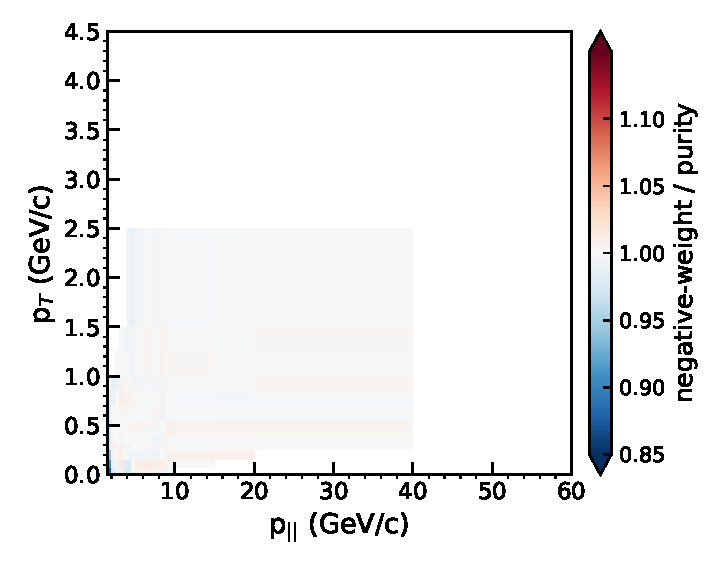
\includegraphics[width=0.62\textwidth]{negweight_ratio_2d}
  \caption{Negative-weight/binned-purity cross-section ratio in populated
    bins of the 2D ME~FHC measurement, with common estimator and seed.
    The median is $\nwMedianBin$ (near-white). Only the low-$p_T$,
    high-background edge bin departs by more than a few percent. Background
    is largest there, and the $\max(0,\cdot)$/structural floor of
    \S\ref{sec:negweight-estimator} governs the result.}
  \label{fig:negweight-ratio}
\end{figure}

\subsection{Propagation through systematics and statistics}
\label{sec:negweight-uq}

Replacing binned subtraction requires reproducing its \emph{uncertainty}
budget as well as the central value. The full 2D ME~FHC covariance was rebuilt
end to end with negative-weight injection and compared to binned purity at
identical settings. The 187-universe systematic ensemble varied genuine
background consistently within each universe instead of freezing it at nominal;
a statistical bootstrap used matched seeds. Agreement is at the level predicted
by the $(D-B)/S$ identity. Overall systematic magnitude has
$\sqrt{\mathrm{tr}}$ ratio $\nwSystRatio$ (negative-weight/purity), and the
statistical ratio is $\nwStatRatio$.
Residuals of \SI{\nwSystResid}{\percent} and \SI{\nwStatResid}{\percent}
% --- each defined from its parent ratio rather than written
% out, so that a later revision of either ratio propagates to it ---
are consistent with ``to within \SI{2}{\percent}'' in \S\ref{sec:method}.
They are bootstrap and classifier-seed sampling noise, with no method bias.
Negative-weight injection reproduces the central cross section \emph{per bin}
(median $\nwMedianBin$, RMS \SI{\nwRmsBin}{\percent}, worst bin
\SI{\nwWorstBin}{\percent}) and covariance \emph{in aggregate}.
The covariance comparison gives two trace ratios; per-bin, correlation and eigenmode
equivalence are not established.

The 2D central-value, closed-form recovery and full covariance comparisons,
together with Stay-Positive robustness on larger extended-fiducial backgrounds,
support negative-weight injection as an unbinned alternative at the 2D scale.
The 2D result and its covariance and the 3D and 4D central values use its refined form
(\S\ref{sec:method-algo}); binned purity remains the treatment of the five-dimensional central
value and its covariance and of the extended-fiducial value.
% Accuracy fix (unscored; director ruling 2026-10-26): "Binned purity remains the default for this note's reproduction
% measurement" was stale; scope as in sec:method-algo and "Scope of the numbers" above.
% Accuracy fix ACC9 (unscored; director ruling 2026-10-26): "the validated unbinned cross-check" dropped. Beside the
% scope above it read as if the 2D result's treatment were only a cross-check. Table tab:estimators-matrix (sec_method.tex)
% gives no negative-weight configuration a cross-check role (its one cross-check, (b), is purity-based), and the drivers' --bkg-mode
% {purity, negweight, negweight-refined} designates none (2d-unfolding/unfold_2d_omnifold_unbinned.py:1362-1377 @ ddf16f10;
% nd-unfolding/unfold_nd_omnifold_unbinned.py:619-630 @ ddf16f10). The 2D validation stays in this paragraph's first sentence.
Negative-weight injection is the
\emph{designated} extended-fiducial baseline (\S\ref{sec:fps}), where
binning-independence and the continuous floor are essential.

\subsection{Which background treatment each production chain uses}
\label{sec:negweight-footing}

Agreement between the two subtractions does not make the choice between them
arbitrary, and the production chains choose differently.

\paragraph{The standard \(N\)-dimensional chain uses purity.}
The entire standard five-dimensional chain uses binned purity
(\S\ref{sec:method-algo}): the central unfold, $169$ vertical-band unfolds,
$18$ detector unfolds and $10$ endpoint unfolds of the re-selected lateral bands. Its background treatment is positively identified, by different evidence for the existing
unfolds and for current production.

For the existing endpoint unfolds, produced in July 2026, purity is established by
elimination. Neither of the two job scripts that could have produced them sets the
driver's background-mode option (\texttt{-{}-bkg-mode}), so the driver ran with its
default, purity; the driver announces its mode only on its negative-weight code
paths, and the logs of these lateral-band unfolds contain the purity code path's
signature line and no mode announcement. The option and the announcements already
existed when the files were produced, so the absence of an announcement is
evidence of purity. Current production fixes the background treatment in a
configuration object that rejects every other mode. The standard job script
passes the option explicitly from that configuration rather than inheriting the
default, and the value is written into the record of every endpoint unfold as it
is produced. This changes how the treatment is documented, not the physics: the
background treatment of a future component can be read from the component itself
rather than inferred from the absence of an option.

The standard chain uses purity by choice, on two grounds
(Ref.~\cite{NoteRecords2026}, \texttt{oi6-oi8-oi126}).
First, mixing background treatments inside one covariance is
worse than either consistent choice: inserting a lateral-band block built with
negative-weight subtraction into a central and vertical set built with purity
subtraction is a mismatch, not an upgrade. Second, switching would have required
rerunning every unfold above and would have invalidated the flux-corrected
covariance, which had just been chosen for use.
This consequence, not the computing cost, decided the choice.
The background treatment has been revisited in two dimensions: the closure test
below is its result, and the 2D result and its covariance use the refined
estimator. For the five-dimensional central value, which still uses purity, the
revisit is open.
% Status of the revisit, stated once here and pointed to from sec. "Purity bias" and "Refined negative-weight
% subtraction" below (director's ruling 2026-10-25, note register round n1, outline question 1): split by result, with
% the earlier tie to the submission date dropped. Sources of the 2D and 5D facts: DECISION-20261024-joseph-adopt-re2-2d-refined.md
% item 1; DECISION-20261023 (second) item 2 (record the revisit as carried out once the rebuilt 2D result is adopted);
% RE-2 integration W7 (DECISION-20261024-joseph-approve-integration-wording-s1-compute-preserve.md), which approved
% wording stating the 2D and 5D facts only; the 5D measurement route has moved to configuration (e), refined negative
% weights (DECISION-20261024-joseph-5d-community-standard-route.md item 5).

% RE-1 integration (DECISION-20261023 items 1-2): C2 of stageF/methods/re1/RE1-REPORT-2.md sec. 2 (readout_2d_full.json,
% c2_supplement.json, c2_cells.json), recomputed by the director (RE1-REPORT-2-RULINGS.md); D2 from sec. 3. OI-6: in
% progress, with C2 as its first result. The 2D switch is decided, not done: the note still prints the purity result.
\paragraph{A two-dimensional closure test with backgrounds.}
Twenty pseudo-experiments at nominal truth (the truth model equals the prior),
with background included and drawn as in the five-dimensional
pseudo-experiments, were unfolded in two dimensions with the purity subtraction
and with refined negative-weight subtraction (a 400-tree, 31-leaf refinement),
both on the same pseudo-data. The yardsticks are the statistical and total
standard deviations, $\sigma_{\mathrm{stat}}$ and $\sigma_{\mathrm{total}}$, of
the purity-based 2D covariance on its 205 reported cells (the quoted covariance when the test ran). The mean difference between
the two treatments exceeds $1\,\sigma_{\mathrm{stat}}$ in 14 of the 205 cells,
at most $5.45\,\sigma_{\mathrm{stat}}$, in the cell
$0.70\le\pT<\SI{0.85}{GeV/c}$, $1.5\le\pPar<\SI{2.0}{GeV/c}$. These cells are
the whole lowest-$\pPar$ row ($1.5$--\SI{2.0}{GeV/c}) and five cells along the
high-$\pT$, low-$\pPar$ boundary. In them, the purity estimate's mean residual
against the truth is $+0.78$ to $+5.89\,\sigma_{\mathrm{stat}}$, above
$1\,\sigma_{\mathrm{total}}$ in one cell ($1.22$); the refined estimate's mean
residual is within $\pm0.44\,\sigma_{\mathrm{stat}}$ in every cell. The
integrated difference between the treatments is \SI{-0.198}{\percent}. In the
median cell, the pseudo-experiments' own spread is $0.46\,\sigma_{\mathrm{stat}}$
(purity) and $0.58\,\sigma_{\mathrm{stat}}$ (refined). The test is a closure with 20 pseudo-experiments, not
a coverage test. On the data, the refined treatment moves the 2D result by at
most $0.497\,\sigma_{\mathrm{total}}$ per cell (median $0.060$), by more than
$1\,\sigma_{\mathrm{stat}}$ in 43 of the 205 cells (at most
$4.26\,\sigma_{\mathrm{stat}}$), and by a median of \SI{0.44}{\percent} per cell
(84th percentile \SI{1.13}{\percent}, at most \SI{10.1}{\percent}); its
integral moves by \SI{-0.139}{\percent}. The 2D result quoted in this note uses the refined
treatment, configuration~(f), with its covariance and its comparison with the published result
rebuilt for it (\S\ref{sec:results}).
% RE-2 integration W7 (approved, DECISION-20261024-joseph-approve-integration-wording-s1-compute-preserve.md): DECISION-20261024-joseph-adopt-re2-2d-refined.md item 1; the -0.139 % and 0.44 % movements
% equal RE2-PARTC-REPORT.md sec. 6 (E_R against E_U: -0.139 %, median 0.440 %, maximum 10.13 %).


\paragraph{What the quoted extended-fiducial number used.}
The $\sigma_{\mathrm{ext}}=\SI{\fpsSigma}{cm^2/nucleon}$ in \S\ref{sec:fps}
was not produced with negative-weight injection.
It comes from the extended-fiducial ME~FHC battery of 2026-06-10, run before the
driver supported negative-weight subtraction. Its ten endpoint unfolds used the
driver's purity default and are recorded as purity controls, not publication inputs
(Ref.~\cite{NoteRecords2026}, \texttt{fps-battery}). The
central value of that battery, \SI{\fpsSigma}{cm^2/nucleon}, is recorded in the
validation ledger with its passed published-region check against the control. No
extended-fiducial production with refined negative-weight subtraction has been run,
so negative-weight injection, the intended extended-fiducial baseline, did not
produce the quoted number.

\paragraph{The extended-fiducial measurement and its control are designated different background treatments.}
For publication, the extended-fiducial analysis designates negative-weight
injection with Stay-Positive refinement as its background treatment. The code fixes
it, and a check stops the run
if any endpoint's recorded mode differs or is missing; the number quoted in
\S\ref{sec:fps} was not produced this way, as stated above. The standard chain uses purity
throughout. Each side of the measurement and matched-control pair therefore has an
internally consistent background treatment; uniformity across the two sides is not claimed.

\subsection{Measured size of the background-treatment choice and its scope}

\paragraph{Measured size.}
On the 2D ME~FHC measurement at full statistics with LightGBM, the estimator of
the quoted 2D central value, the two covariances differ by one to two percent. The $187$-universe systematic
$\sqrt{\mathrm{Tr}}$ ratio is $\nwSystRatio$, from
\SI{2.9828e-39}{cm^2/nucleon} negative-weight and
\SI{3.0242e-39}{cm^2/nucleon} purity. Matched-seed statistical covariance has
ratio $\nwStatRatio$, from \SI{1.7260e-40}{cm^2/nucleon} and
\SI{1.7576e-40}{cm^2/nucleon}, respectively. With the histogram backend, the
real-data totals agree to \SI{\nwPctTot}{\percent}, with per-bin median $\nwMedianBin$ and
\SI{\nwRmsBin}{\percent} RMS. These are the comparisons of
\S\ref{sec:negweight-2d} and \S\ref{sec:negweight-uq}, with the operands of
each ratio given.

\paragraph{Displacement across universes.}
The displacement argument rests on a \emph{measured} input; it assumes no
identity of continuous estimands. The constructions share bin masses in the
binned limit (\S\ref{sec:negweight-binned}) but differ by within-bin shape
terms (\S\ref{sec:negweight-estimator}). Switching background treatment produces a measured net per-universe displacement of order \SI{0.1}{\percent}, including residual
and shape effects, at this measurement's sub-percent genuine-background scale.
Systematic covariance measures spread across universes about their own mean. Similar
small shifts of each universe leave that spread nearly unchanged, explaining
the $187$-universe ratio $\nwSystRatio$, far from the purity correction's
${\sim}\SI{3}{\percent}$. This argument connects a handful-of-universes
comparison to the $187$-universe covariance; the full $187$-universe rebuild
in \S\ref{sec:negweight-uq} tests it at 2D and passes.

\paragraph{Scope.}
The measured agreement concerns these 2D systematic and statistical covariances at
the stated configurations. It is not a theorem that the two background treatments
give the same covariance, because the underlying estimands are not pointwise
identical, and covariance equivalence for the continuous estimator or in five
dimensions is not established. The five-dimensional evidence is limited to the
following two-universe spot check.

\paragraph{Limits of the five-dimensional evidence.}
There is no full five-dimensional $187$-universe comparison of the two background
treatments at the publication configuration ($5$ iterations, LightGBM). The spot
check uses one iteration and the histogram backend on the stored five-dimensional
universe file: under both treatments \texttt{2p2h:0} gives $3.014\times10^{-38}$ with
per-bin median $1.0005$, and \texttt{MaCCQE:0} differs by \SI{-0.03}{\percent}
with median $0.9990$. Together with the displacement argument and the full-statistics
2D result, this supports quoting the standard chain with purity subtraction, with
its background treatment stated. It does not show that the background treatment
is irrelevant in five dimensions, which would require the full comparison. Raw
negative weights destabilize the exact-split backend
(\S\ref{sec:negweight-estimator}), but the standard chain uses LightGBM, so
neither treatment risks that pathology here; the choice is safe, though not
shown to be immaterial.

\subsection{Five-dimensional pseudo-experiments with both background treatments}

The five-dimensional validation (\S\S\ref{sec:val-fiveaxis}--\ref{sec:val-departure})
reports end-to-end tests of both background treatments: purity bias in the highest-$W$ column at nominal truth, its reduction with refined negative-weight subtraction, the data difference, and the estimator with higher refinement capacity, configuration (e), which gives the 3D and 4D central values but not the quoted 5D central value; the quoted 2D central value uses the same refinement capacity, in configuration (f).

\paragraph{Purity bias.}
Purity bias is 8--12 statistical standard deviations; signal-only experiments
close. Subtraction is exact per reconstructed bin, but the widest bin
($W\ge\SI{3}{GeV}$, background \SI{13}{\percent} of signal) contains background
shape resolved by the unbinned classifier and missed by bin-uniform purity.
The within-bin shape term of \S\ref{sec:negweight-estimator} is therefore
measurable, and it is direct evidence for revisiting the five-dimensional background
treatment (\S\ref{sec:negweight-footing}). Comparing five-dimensional
purity with refined negative-weight subtraction on data is the cheapest estimate of
its size on data.
% Source: docs/orchestration/OUTCOME-20260925-s5c-purity-background-bias-at-high-W.md; KNOWN_ISSUES 75.
% Heading date (2026-09-25) and the numbers repeated in sec_validation.tex removed (lane 3 App. B #7):
% highest-$W$ column \SIrange{3.5}{4.1}{\percent} low, highest-$\Eavail$, highest-$W$ cell \SI{1.7}{\percent} high.

\paragraph{Refined negative-weight subtraction.}
Refinement used the unfold's deterministic GBDT configuration, independent
injection and subtraction halves of background simulation, and bootstrap
replicas that individually resampled every pseudo-event and refit refinement.
It preserves the signed total to $3\times10^{-6}$ and clips
\SIrange{0.01}{0.05}{\percent} of events. Corner bias falls from
\SI{1.66}{\percent} to \SI{0.24}{\percent}, but residuals in some joint cells
fail the nominal closure criterion, which allows none of the 153 reported quantities a mean
residual beyond 3.6 standard errors of the mean ($|t|>3.6$, the two-sided 5\% level, Bonferroni-corrected
over the 153), or beyond half its bootstrap standard deviation with $|t|>3$.
% Note register round n1, batch n1-F: the criterion stated (state/s5n/contract.json, stage_1_development, controls C3
% and C6; OUTCOME-20260925-s5n-stage1-development-fail.md sec. 2, C3 FAIL; nd-unfolding/s5n_analyze_dev.py:112-149);
% "predeclared" dropped, since the result is a failure.
The data difference's sign
pattern matches simulated purity bias at an order of magnitude smaller size;
the difference is method sensitivity, not a measured bias. With either treatment, the estimator does not follow generator-sized $\Eavail$ shape changes.
No coverage test was run.
Reducing one bias does not itself qualify an uncertainty, so this result does not close the revisit of the
five-dimensional background treatment (\S\ref{sec:negweight-footing}).
% Search: s5n coverage; coverage test; coverage verdict; no validation seed was run (OUTCOME-20260925-s5n-stage1-development-fail.md:13) @ ddf16f1087d7
% Source: docs/orchestration/OUTCOME-20260925-s5n-stage1-development-fail.md; VL151, VL152.
% Heading date (2026-09-25) and numbers repeated in sec_validation.tex removed (lane 3 App. B #7):
% highest-$W$ bias falls from \SIrange{-3.5}{-4.1}{\percent} to \SIrange{0.11}{0.24}{\percent};
% residual of up to about \SI{1}{\percent}; on the data the two footings
% differ by a median of \SI{0.36}{\percent} and at most \SI{1.4}{\percent}.

\paragraph{Refinement capacity.}
Stay-Positive classifier underfitting causes the residual nominal bias of the refined subtraction. At the unfold's GBDT setting (100 trees, 8 leaves), the
positive-weight probability is underfit, leaving up to \SI{4}{\percent}
reco-level subtraction error per $(\Eavail,W)$ reco cell. With 400 trees and 31 leaves,
error falls to \SI{1.7}{\percent}, paired truth-level bias falls by more than
\SI{80}{\percent} in every affected cell, and nominal background-inclusive
closure passes on 20 development and 40 fresh pseudo-experiments.
Splitting background simulation into independent injection and subtraction
halves is not the cause.
% Source: docs/orchestration/DIAGNOSIS-20260926-s5e-oi192-estimator.md §5;
% docs/orchestration/OUTCOME-20260926-s5e-oi192-diagnosis-and-candidate.md; VL153, VL154.
% Heading date (2026-09-26) removed. Moved to the pointer above: "The higher-capacity refinement
% is not adopted: the estimator it feeds failed a stability test on the data (\S\ref{sec:validation})."

\paragraph{Background treatment and choice of covariance.}
The choice of background treatment and the choice of covariance are independent,
and nothing in this appendix selects a five-dimensional covariance for use. The
lateral-band component from re-selected event loops is built, with five bands and
ten endpoint unfolds whose distinct checksums are listed in the record of the
covariance used in this note. That five-axis covariance is used although it does not
meet the acceptance criteria of its specification, and the use covers only that file and
its projection (\S\ref{sec:eavailw-adopted}). Neither fact follows from this appendix, and the appendix
needs neither. The choice of background treatment settles one of the conditions for using
a component; every other condition still applies.
% Plain status of the use of the five-axis covariance as printed at sec:eavailw-adopted (sec_5d.tex): it does not meet
% its specification's acceptance criteria, and its use covers only this file and its projection.

\section{Detector-response-mismatch closure (protocol implemented; not yet run)}
\label{app:response-mismatch}

The truth-shape and hidden-variable closures in \S\ref{sec:validation} test
recovery of deliberately modified event populations. They do not directly test
truth-distribution bias from a mismatch between the pseudo-data detector
response and OmniFold's nominal response. Kevin McFarland suggested this
distinction and proposed stressing the hadronic record, especially for
quasielastic events, to inspect low-$W$ bias (private communication).

\paragraph{Reconstruction-only test implemented in the pipeline.}
The first-stage diagnostic uses the ordinary five-dimensional closure sample.
After copying pseudo-data arrays, before background mixing or classifier
training, it changes only the reconstructed pseudo-data record
\begin{equation}
  \Eavail^{\mathrm{pseudo}} \longrightarrow
  (1+\epsilon)\Eavail^{\mathrm{pseudo}} .
\end{equation}
The nominal reconstructed simulation, all truth coordinates, event weights,
and event membership stay fixed. The pseudo-data therefore have a deliberately
incompatible conditional response; OmniFold still uses the nominal response.
The protocol requires both signs of $\epsilon$, at an amplitude fixed before the results
are examined. A documented hadronic-response variation or a quantified assumption should justify
that amplitude; the inherited factor in reconstructed $\Eavail$ is not enough on its own.

Outputs include the full five-dimensional unfolded/reference residual,
one-dimensional $\Eavail$ and $W$ projections, and an $(\Eavail,W)$ ratio map.
The primary observable is signed bias versus $W$, reporting $W<\SI{1.1}{GeV}$
separately from the high-$W$ tail. The global integral is a control rather than the decision statistic.
The implementation runs only as a closure on pseudo-data and only on the five observables, and it
cannot be combined with truth reweighting or bootstrapping. It labels every output as a diagnostic
that must not be quoted.
% Guards: nd-unfolding/unfold_nd_omnifold_unbinned.py:671-672 (--closure: MC reco as pseudo-data) and :692-711
% (requires --closure and exactly --axes eavail,q3,W; refuses truth reweighting and --bootstrap-seed; output basename
% NONQUOTABLE-DIAGNOSTIC.) @ 1a015eef.

\paragraph{Physically correlated follow-up.}
The reconstruction-only arm is intentionally cheap and adversarial; it is not a
detector model. A more faithful follow-up would select quasielastic events,
shift leading-nucleon energy up and down, and recompute reconstructed
$\Eavail$, $q_{3}$, $W$, and any affected selection from the altered low-level
record. The current scalar event-loop outputs lack the information for that recomputation,
so this arm needs dedicated diagnostic output from the event loop.
It is deferred unless the reconstruction-only test shows material bias or the
collaboration asks for the stronger response model.

\paragraph{Status and interpretation.}
This appendix records a validation protocol, not a result or an uncertainty
component. No
response-mismatch output has been produced and no pass threshold has been set. The test leaves the quoted central value and the current covariance construction unchanged. A small observed bias would support stability of the
$(\Eavail,W)$ interpretation only within the tested response envelope. A large
bias would require a decision on the response model or an uncertainty
component, and would not be absorbed silently into a non-closure error.
% Search: response-mismatch; response mismatch; mismatch closure; RESPONSE_MISMATCH_CLOSURE; NO RESULT EXISTS (HANDOFF-20260922-gbdt-cold-start.md:316); not yet run (EVIDENCE-MAP-20261019.md:80) @ ddf16f1087d7

\section{The MINERvA measurement-dimensionality survey}
\label{app:landscape}

The survey behind Fig.~\ref{fig:landscape} lists MINERvA differential cross-section measurements through the listed 2025 entries, with references and how many kinematic variables each headline result unfolds simultaneously. Recent additions follow; the inventory is not exhaustive through 2026.

{\small
\begin{longtable}{@{}clcl@{}}
  \caption{MINERvA differential cross-section survey used for the landscape figure: the number of
  kinematic variables unfolded simultaneously (Dim.), classified from each
  analysis's headline differential result. Channels: CC-inclusive (incl.),
  CCQE/QE-like incl.\ transverse kinematic imbalance (QE), pion production CC
  and coherent ($\pi$), deep-inelastic / kaon (DIS), electron-neutrino
  ($\nu_e$), nuclear-target ratio (ratio).}
  \label{tab:landscape}\\
  \toprule
  Year & Channel; observables & Dim. & Ref. \\
  \midrule
  \endfirsthead
  \toprule
  Year & Channel; observables & Dim. & Ref. \\
  \midrule
  \endhead
  \midrule \multicolumn{4}{r}{\emph{continued\ldots}}\\ \endfoot
  \bottomrule
  \endlastfoot
  2013 & QE; $\nu_\mu$ CCQE $\pT,\pPar$            & 2 & \cite{MINERvA:2013qe} \\
  2013 & QE; $\bar\nu_\mu$ CCQE $\pT,\pPar$        & 2 & \cite{MINERvA:2013qebar} \\
  2014 & ratio; CC on C/Fe/Pb to CH               & 1 & \cite{MINERvA:2014ratio} \\
  2014 & $\pi$; coherent $\pi^\pm$ (total \& diff.) & 1 & \cite{MINERvA:2014coh} \\
  2015 & $\pi$; CC $1\pi^+$ ($T_\pi$, $\theta_\pi$) & 1 & \cite{MINERvA:2015ydy} \\
  2015 & QE; $\mu$+p final states                 & 1 & \cite{MINERvA:2015mup} \\
  2015 & $\pi$; $\bar\nu_\mu$ single $\pi^0$       & 1 & \cite{MINERvA:2015pi0} \\
  2016 & $\nu_e$; CCQE-like on CH                  & 2 & \cite{MINERvA:2016nueqe} \\
  2016 & $\pi$; $\nu_\mu/\bar\nu_\mu$ pion prod.   & 2 & \cite{MINERvA:2016pion} \\
  2016 & DIS; partonic nuclear effects            & 2 & \cite{MINERvA:2016dis} \\
  2016 & DIS; CC $K^+$ production                  & 1 & \cite{MINERvA:2016kaon} \\
  2017 & $\pi$; CC single $\pi^0$                  & 2 & \cite{MINERvA:2017pi0} \\
  2017 & QE; nuclear-dependence (multi-target)     & 1 & \cite{MINERvA:2017Adep} \\
  2018 & QE; $\bar\nu_\mu$ QE-like $\pT,\pPar$     & 2 & \cite{MINERvA:2018hba} \\
  2018 & QE; $\mu$-p mesonless TKI                 & 2 & \cite{MINERvA:2018tcb} \\
  2018 & $\pi$; coherent $\pi^\pm$ on C            & 2 & \cite{MINERvA:2018coh} \\
  2019 & QE; quasielastic-like $\nu_\mu$           & 2 & \cite{MINERvA:2019qe} \\
  2019 & $\pi$; $\bar\nu_\mu$ single $\pi^-$       & 2 & \cite{MINERvA:2019pim} \\
  2020 & incl.; CC-incl $\langle E_\nu\rangle\!\sim\!3.5$ GeV $\pT,\pPar$ & 2 & \cite{MINERvA:2020jwd} \\
  2020 & QE; nuclear binding \& TKI               & 2 & \cite{MINERvA:2020cgh} \\
  2020 & QE; high-statistics QE-like              & 2 & \cite{MINERvA:2020qehs} \\
  2020 & $\pi$; CC $\pi^0$ nuclear effects        & 1 & \cite{MINERvA:2020pi0} \\
  2021 & incl.; CC-incl $\langle E_\nu\rangle\!\sim\!6$ GeV $\pT,\pPar$ \textbf{(target)} & 2 & \cite{MINERvA:2021owq} \\
  2022 & QE; QE-like $\pT,\pPar,\Sigma T_p$ (triple-diff.) & 3 & \cite{MINERvA:2022qelike3d} \\
  2022 & incl.; CC-incl low-$q_{3}$ ($\Eavail$, $q_{3}$) & 2 & \cite{MINERvA:2022incl} \\
  2023 & $\pi$; CC $1\pi^+$ (multi-target)        & 2 & \cite{MINERvA:2023ccpi} \\
  2023 & $\pi$; coherent $\pi^+$ (multi-target)   & 1 & \cite{MINERvA:2023coh} \\
  2023 & QE; $\bar\nu_\mu$ multi-neutron low-$\Eavail$ & 1 & \cite{MINERvA:2023lowEavail} \\
  2024 & $\nu_e$; low-$Q^2$ ($\Eavail$, $\pT$)    & 2 & \cite{MINERvA:2023avz} \\
  2025 & QE; $A$-dependence TKI (multi-target)    & 2 & \cite{MINERvA:2025tki} \\
  \midrule
  2026 & \textbf{this work}; unbinned $\pT,\pPar$            & 2 & --- \\
  2026 & \textbf{this work}; unbinned $\pT,\pPar,\Eavail$    & \textbf{3} & --- \\
  2026 & \textbf{this work}; unbinned $\pT,\pPar,\Eavail,q_{3}$ & \textbf{4} & --- \\
  2026 & \textbf{this work}; unbinned $\pT,\pPar,\Eavail,q_{3},W$ & \textbf{5} & --- \\
\end{longtable}
}

\paragraph{Additional recent measurements.} The low-/medium-energy comparison of quasielastic-like cross sections reports three simultaneous axes, $\pT$, $\pPar$, and available recoil energy \cite{MINERvA:2026qeleme}; it is a direct dimensional precedent with a different signal from our inclusive result. The shallow-inelastic measurement reports one-dimensional neutrino and antineutrino cross sections \cite{MINERvA:2026sis}. Other measurements report single-differential charged-pion production down to zero pion kinetic energy \cite{MINERvA:2026pion} and inclusive antineutrino cross sections versus $\pT$ on several targets~\cite{MINERvA:2026antinu}. Counting measured observables does not count simultaneously unfolded axes. These channel-specific additions are not plotted in Fig.~\ref{fig:landscape}.

% The PET appendices (sec_pet.tex with sec_pet_campaigns.tex, and app_cstat.tex) moved to the
% companion note pet_note.tex on 2026-10-12, at Joseph's request, so that this note can accompany the
% scalar (GBDT) result on its own. This appendix keeps the label every PET pointer in this note
% uses, and states PET's status where this note's readers meet it. The status sentences are those of
% sec_pet.tex's opening paragraph.
\section{Point-cloud (PET) studies: companion note}
\label{sec:pet}

The point-cloud transformer (PET) studies are reported in a companion note built from the same
sources (\texttt{docs/analysis-note/pet\_note.tex}, \repolink). It carries what were this note's
appendices on the point-cloud representation and PET method development --- including the completed
simulation studies of PET design and the exploratory PET--GBDT comparison on the same events --- and
on the full-event $C_{\rm stat}$ construction, together with their repository records and audit
trail. References from this note into the companion note name its sections by title.

All PET results are diagnostic and method development. No PET covariance,
historical recoil-only or full-event, is adopted as a publication uncertainty
product. The full-event central/statistical pairing was declined on 2026-08-20
and remains declined. Reconsideration requires estimator-equivalence and
coverage evidence; no branch was chosen.

\section{Repository records cited in this note}
\label{app:provenance}

Several statements in this note rest on records in the analysis repository rather than on anything
a reader can recompute from the published inputs. Those records are collected here rather than
inlined, for two reasons. A repository path is not usable by a reader outside the collaboration, so
in the body it interrupts a physics argument with a string that cannot be followed; and gathering
them in one table means a path that moves has one place to be corrected instead of five.
All paths below are relative to the code repository, \repolink, and are set breakably so they stay
inside the text block.

\textbf{This appendix is not the reproduction path.} What an external reader would need in order to
recompute the quoted numbers --- the arrays, edges, orderings, masks, units, projection matrices and
generator predictions, with one worked example --- is specified separately in
App.~\ref{app:release}, together with a measured statement of which of those objects exist today and
which do not.

\textbf{This appendix is provenance, not evidence.} Nothing here is a result, and no statement in
the body becomes stronger because its record is listed. Where a claim depends on a record whose own
limitations matter---most importantly the adopted covariance's four measurements
(\S\ref{sec:eavailw-adopted})---those limitations are stated at the claim, not delegated here.

The tags are stable; the paths are current as of 2026-10-06. Rows are ordered by the
section that cites them. Table~\ref{tab:prov-paths} lists records with a repository path;
Table~\ref{tab:prov-trackers} lists tracker rows and code identifiers that have no
document of their own.

{\small
\begin{longtable}{@{}llp{0.50\textwidth}@{}}
\caption{Repository records with a path.}\label{tab:prov-paths}\\
\toprule
Tag & Cited at & Record \\
\midrule
\endfirsthead
\toprule
Tag & Cited at & Record \\
\midrule
\endhead
\midrule \multicolumn{3}{r}{\emph{continued\ldots}}\\ \endfoot
\bottomrule
\endlastfoot
\texttt{coverage-fixed-truth} & \S\ref{sec:coverage} &
  see below \\
\texttt{coverage-toys} & \S\ref{sec:val-other} &
  see below \\
\texttt{flux-repair} & \shortstack[l]{\S\ref{sec:3d-models}, \S\ref{sec:eavailw-band},\\
  App.~\ref{app:release-schema}, App.~\ref{app:history}} &
  see below \\
\texttt{q3-excess} & \S\ref{sec:4d} &
  \texttt{nd-unfolding/}\allowbreak\texttt{q3\_excess\_projection.py} (comparator: Tune~v1 prior,
  weights \texttt{w\_truth}); produces Fig.~\ref{fig:q3excess} \\
\texttt{eavailw-excess} & Fig.~\ref{fig:eavailWexcess} &
  \texttt{nd-unfolding/}\allowbreak\texttt{excess\_eavail\_W.py} (cell-integrated differences;
  comparator weights \texttt{w\_truth}) \\
\texttt{z-adoption} & \S\ref{sec:eavailw-construction}, App.~\ref{app:release-audit} &
  see below \\
\texttt{joint-5d} & \S\ref{sec:joint5d}, Table~\ref{tab:joint5d} &
  see below \\
\texttt{retracted-values} & \S\ref{sec:pet}, App.~\ref{app:history} &
  \repopath{docs/orchestration/INDEX-retracted-and-superseded-values.md} \\
\texttt{pet-pairing} & \S\ref{sec:pet}, \S\ref{app:cstatlimit} &
  see below \\
\texttt{pet-closure-legacy} & \S\ref{sec:pet-abs} &
  ruling of 2026-08-21;
  \repopath{docs/orchestration/DETERMINATION-20260819-lanec-petclosure-is-legacy.md} \\
\texttt{pet-projection-figure} & \S\ref{sec:pet-projection} &
  see below \\
\texttt{variance-sources} & Table~\ref{tab:variance-sources} (\S\ref{sec:variance}) &
  see below \\
\texttt{rank-inversion} & \S\ref{sec:nd-declarations} &
  \repopath{docs/orchestration/RANK-AND-INVERSION-20260810.md}; the predeclared rank cut itself is
  a statistics decision recorded in \texttt{docs/}\allowbreak\texttt{STATVAL\_REPAIR.md} \\
\texttt{closure-scripts} & \S\ref{sec:closure} &
  \texttt{uq/closure/}\allowbreak\texttt{closure\_truth\_reweight.py} (\S\ref{sec:closure-tr});
  \texttt{uq/closure/}\allowbreak\texttt{closure\_hidden\_var.py} (\S\ref{sec:closure-hv});
  \texttt{uq/closure/}\allowbreak\texttt{closure\_alt\_model.py} (\S\ref{sec:closure-alt}) \\
\texttt{cstat-recompute} & \S\ref{app:cstatlimit} &
  see below \\
\texttt{negweight-toy} & \S\ref{app:negweight} &
  \repopath{docs/orchestration/receipts/RECEIPT-negweight-toy-20260821.json} \\
\texttt{negweight-hpss} & \S\ref{app:negweight} &
  see below \\
\texttt{negweight-audit} & \S\ref{app:negweight} &
  \repopath{docs/orchestration/AUDIT-FINDINGS-20260731.md}, tier~A, finding J22 \\
\texttt{gbdt-closeout} & \S\ref{app:negweight} &
  \repopath{docs/orchestration/RUNBOOK-20260807-gbdt-closeout.md} \S2.1--2.2 \\
\texttt{oi6-oi8-oi126} & \S\ref{app:negweight} &
  see below \\
\texttt{p4-verifier} & \S\ref{app:negweight} &
  \repopath{docs/orchestration/runs/standard-p4-verifier/} \\
\texttt{fps-battery} & \S\ref{app:negweight} &
  see below \\
\texttt{z-projection} & App.~\ref{app:release-identities} &
  see below \\
\texttt{z-assembly} & App.~\ref{app:release-audit} &
  \texttt{nd-unfolding/}\allowbreak\texttt{z\_assembly.py} (implements
  Eqs.~\eqref{eq:zassembly}--\eqref{eq:zinflation}); the same algebra is asserted independently
  of the producer \\
\texttt{z-conditioning} & App.~\ref{app:release-audit} &
  see below \\
\end{longtable}
}

\noindent Tags marked ``see below'' carry records or context too long for the
column above, so they are given here at full width.

\begin{description}[leftmargin=0pt,itemsep=3pt]
  \item[\texttt{coverage-fixed-truth}.] Pre-registration
    \repopath{docs/orchestration/PREREG-20261005-2d-fixed-truth-coverage.md} (amendments 1--2);
    outcome \repopath{docs/orchestration/OUTCOME-20261005-2d-fixed-truth-coverage-fail.md};
    \texttt{VALIDATION\_LEDGER.md} row \texttt{VL169}; \texttt{KNOWN\_ISSUES.md} row 84. Toy
    driver, extractor and scorer in \texttt{2d-unfolding/}\allowbreak\texttt{uq/}\allowbreak\texttt{coverage\_fixed\_truth/}; receipts,
    including the independent recomputation and the node-hour ledger
    ($\approx\covTwoDNodeH$ CPU node-h), in
    \repopath{docs/orchestration/state/coverage-2d-20261005/}. The band scored is \texttt{VL162}
    (\texttt{uq/bootstrap\_MEFHC\_300/uq\_covariance\_boot300.root}), since superseded by
    \texttt{VL170} (\texttt{uq/bootstrap\_MEFHC\_300\_vl170/}; rollup \texttt{VL172},
    \repopath{docs/orchestration/state/ki84-adopt-20261006/}). The post hoc, descriptive rescoring of
    these toys against \texttt{VL170} is in \repopath{docs/orchestration/state/ki84-rebuild-20261006/}.
  \item[\texttt{coverage-toys}.] Launcher \texttt{sbatch\_coverage\_toys\_MEFHC\_200.sh}; rollup
    \texttt{uq/coverage\_toys.py}; summary \texttt{uq/coverage/}\allowbreak\texttt{coverage\_summary.txt}.
    Each toy runs the driver with \texttt{-{}-closure} and \texttt{-{}-bootstrap-seed $k$}; the
    stored truth histogram is \texttt{hTruthXSec2D}, fluctuated through \texttt{w\_truth}.
  \item[\texttt{flux-repair}.] \texttt{KNOWN\_ISSUES.md} rows 82 (GiBUU sample stops at
    $E_\nu\approx\SI{20}{GeV}$) and 83 (GENIE/NuWro flux mis-sampling); repair and rebuild of
    2026-09-27, \texttt{VALIDATION\_LEDGER.md} rows \texttt{VL156}--\texttt{VL160} (\texttt{VL159}:
    3D integrated-rate shares; \texttt{VL160}: Valencia-2p2h fill), superseding
    \texttt{VL35}--\texttt{VL38}; receipt
    \repopath{docs/orchestration/state/s5p/stage7/generator-context/generator-context-receipt.json}.
  \item[\texttt{z-adoption}.] The adoption itself at
    \repopath{docs/orchestration/DECISION-20260920-joseph-adopts-z-cv-under-the-6.4-exception.md};
    the seed measurements at
    \repopath{docs/orchestration/EVIDENCE-20260920-sproj-resolution-floor-and-seed-effect.md}
    and \repopath{docs/orchestration/state/SEED-EFFECT-20260920.json}; and the
    withdrawal of the lower-bound reading at
    \repopath{docs/orchestration/CORRECTION-20260920-lower-bound-inference-withdrawn.md}.
    Adoption recorded 2026-09-20; the predeclared magnitude criterion is \emph{cause~3}'s
    $M(\mathrm{ii})$ in the internal dependency register, computed by the 2026-09-20 campaign
    for the two companion products only.
  \item[\texttt{joint-5d}.] The frozen design is amendment~7 at commit \texttt{4f5a613f}; the
    result, with its six conditions verbatim, at
    \repopath{docs/orchestration/RECORD-20261005-s5p-joint-5d-inference-result.md}; the evaluated
    outputs at \repopath{docs/orchestration/state/s5p/stage7/joint/joint-evaluate.json}
    (sha256 \texttt{b9604502}) and \texttt{robust-labels.json}; the independent recomputation
    (verdict AGREE, 1379 of 1379 rows) on branch \texttt{s5p-parallel-recompute-20260928} at
    \texttt{466b427b} (\texttt{REPORT-20261005-s5p-recompute-final-verification.md} \S8);
    the lost-draw recovery at
    \repopath{docs/orchestration/RECORD-20261006-s5p-lost-seed-recovery-resolution.md}, with its
    independent cross-check (856 of 856 quantities; frozen-shift reading only, on branch
    \texttt{s5p-parallel-recompute-20260928} at \texttt{00009056}); the owner's disposition at
    \repopath{docs/orchestration/DECISION-20261005-s5p-recompute-extension-and-lost-seed-recovery.md}
    \S5; and the fresh-checkout replay in \texttt{reproduction/s5p/} (tier~D). Open item
    \texttt{OI-193}.
  \item[\texttt{pet-pairing}.] \texttt{OI-126} in \texttt{docs/OPEN\_ITEMS.md}.
    The 2026-08-20 ruling: the central/statistical pairing is declined, no PET
    total covariance is adopted for publication, PET remains a
    diagnostic and method-development result, and reconsideration requires
    estimator-equivalence \emph{and} coverage evidence --- coverage being a
    different object from verifying the construction.
    Ratification rests with the estimator's owner and the covariance-construction reviewer, and
    the open item recording the question (\texttt{OI-126}) is not closed by
    App.~\ref{app:cstatlimit}.
  \item[\texttt{pet-projection-figure}.] \texttt{ISSUE-59} in
    \texttt{KNOWN\_ISSUES.md} (fixed 2026-09-23; \texttt{pet\_cloud\_projection\_xsec} regenerated) and the corrected values at
    \texttt{nd-unfolding/products/pet/fullcloud/pointcloud\_projection\_summary.json},
    which holds the three $\Eavail$ projections (\texttt{pet\_cloud\_hascloud},
    \texttt{pet\_stored\_hascloud}, \texttt{pet\_stored\_full}); method and
    reproduction at \texttt{nd-unfolding/pet/POINTCLOUD\_PROJECTION.md}.
  \item[\texttt{variance-sources}.] Code pointers, one per row of
    Table~\ref{tab:variance-sources}. Training-seed variation:
    \texttt{seedscan/analyze\_seedscan.py}; \texttt{uq/seedscan\_lgbm\_ml/
    uq\_covariance\_ml.root}. Poisson bootstrap: \texttt{unfold\_2d\_omnifold\_unbinned.py}
    (\texttt{-{}-bootstrap-seed}, \texttt{-{}-seed}); \texttt{uq/analyze\_uq.py};
    \texttt{uq/bootstrap\_MEFHC\_300/ uq\_covariance\_boot300.root}. Universes:
    \texttt{runEventLoopOmniFold.cpp} (\texttt{MNV101\_DUMP\_UNIVERSES});
    \texttt{unfold\_2d\_omnifold\_unbinned.py -{}-universe BAND:IDX};
    \texttt{uq/analyze\_universes.py} (\texttt{-{}-add-norm 0.014}). MAT reference:
    \texttt{uq/verify\_matcorr\_vs\_mnvh1d.py}. Block sum:
    \texttt{compare\_to\_paper\_fullcov.py} (\texttt{-{}-omnifold-cov}).
  \item[\texttt{cstat-recompute}.] Every figure in App.~\ref{app:cstatlimit} is derived from
    committed artifacts, and the per-cell arrays behind the aggregates are published with them:
    the family spread and its per-replica values in
    \texttt{state/probe-oi126-band-Rpush-sigma-20260815}; the training-versus-extraction split,
    its control region, and the thresholds fixed before that comparison ran in
    \texttt{state/probe-oi126-push-vs-extraction-20260815} and the predeclaration beside it; the
    $\mathrm{Poisson}(1)$ verification of the targets in
    \texttt{state/RECEIPT-20260815-oi126-mechanism-narrowing} and
    \texttt{state/probe-oi126-zero-fraction-per-column-20260815}; the band geometry, acceptance,
    share of integral and the external comparison in
    \texttt{state/RECEIPT-20260815-cstat-tail-geometry-and-weighting-correction}; and the two
    per-cell relative standard deviations tabulated there as fields of
    \texttt{state/p5a-nominal-vs-cstat-family-percell-20260815}, recomputable from that receipt's
    own shipped per-cell array. No share-of-total figure from that receipt is used
    (App.~\ref{app:history}). The members' input file is measured in
    \texttt{state/gate5-source-npz-verified-20260813}, which should be cited for that purpose in
    preference to the members' own recorded input digest.
  \item[\texttt{negweight-hpss}.]
    \repopath{docs/orchestration/RECEIPT-20260821-negweight-hpss-durability.md}.
    The real-data products behind the twelve
    production values are archived and were restored end to end from tape under a tested
    recovery route; the synthetic-toy values come from a committed, fully deterministic
    script that reproduces all four on re-run (\texttt{negweight-toy}). Two provenance
    limits travel with the production numbers: the driver was uncommitted when those
    outputs were written, so the executing revision is corroborated by a version-distinct
    log string rather than pinned by a digest, and no output carries a producing job
    identifier, which no later run can supply.
  \item[\texttt{oi6-oi8-oi126}.]
    \repopath{docs/orchestration/DECISION-20260815-joseph-oi6-oi8-oi126.md}. The purity
    footing of the standard chain was raised as a question --- whether the locked
    instruction that $N$-D production runs \texttt{negweight-refined} reaches the
    standard-phase-space chain, or only its extended-fiducial form --- and answered in
    favour of purity on 2026-08-07 (\texttt{gbdt-closeout}) and again, after the
    alternative was costed, on 2026-08-15.
  \item[\texttt{fps-battery}.] FPS ME~FHC battery of 2026-06-10, scheduler job
    \texttt{54244120} (\texttt{VALIDATION\_LEDGER.md}, ``FPS MEFHC battery''). The
    negative-weight driver code did not land until 2026-07-11 (commit \texttt{cf8a4a6})
    and the \texttt{-{}-bkg-mode negweight-refined} launcher flag not until 2026-07-20.
    Both FPS unfold launchers omitted \texttt{-{}-bkg-mode} entirely, so the ten endpoint
    unfolds ran on the driver default \texttt{-{}-bkg-mode=purity}; they are recorded as
    purity controls at
    \texttt{nd-unfolding/uq\_fps/corrected/}\allowbreak\texttt{FPS\_UQ\_CORRECTED\_STATE.md}.
  \item[\texttt{z-projection}.]
    \repopath{docs/orchestration/state/PROJ-20260920-m1-publication-receipt.json}
    and \repopath{docs/orchestration/state/PROJ-20260920-binding-check.json}.
  \item[\texttt{z-conditioning}.] Cutoff scan:
    \texttt{PLAN-20260918-scalar5d-publication-completion.md} \S16.1a (diagnostic projection, same
    $M$); independent scan of the publication bytes: \texttt{VALIDATION\_LEDGER.md} row
    \texttt{VL145} (publication and diagnostic $42\times42$ matrices bitwise identical). Default
    cutoff $10^{-12}$ is hardcoded in \texttt{project\_cov\_nd.py}.
\end{description}

{\small
\begin{longtable}{@{}llp{0.25\textwidth}p{0.30\textwidth}@{}}
\caption{Tracker rows and code identifiers: \texttt{KNOWN\_ISSUES.md} rows,
\texttt{VALIDATION\_LEDGER.md} rows (VL), open items (OI), issues, audit findings,
gates and receipt fields, commits and job identifiers, and code symbols.}\label{tab:prov-trackers}\\
\toprule
Tag & Cited at & Record & Content \\
\midrule
\endfirsthead
\toprule
Tag & Cited at & Record & Content \\
\midrule
\endhead
\midrule \multicolumn{4}{r}{\emph{continued\ldots}}\\ \endfoot
\bottomrule
\endlastfoot
\texttt{pet-code} & \S\ref{sec:pet-inputs}, \S\ref{sec:pet-abs} &
  \texttt{nd-unfolding/pet/}\allowbreak\texttt{minerva\_pet\_dataloader.py}; \texttt{MultiFold.reweight}
  (\texttt{omnifold\_nn/omnifold/}\allowbreak\texttt{omnifold.py}); \texttt{extract\_cross\_section\_nd}
  (\texttt{nd-unfolding/xsec\_nd.py}) &
  the dataloader slices off PDG before classification; the full-sample reweight;
  the standard extraction \\
\texttt{cstat-family} & \S\ref{sec:pet-syst}, \S\ref{app:cstatlimit} &
  \texttt{VL132} (the Gate-5 family); \texttt{CSTAT-R7} &
  the full-event extended-fiducial 50-member replica family; the design document specifying
  $N=100$ labels a family of this size \texttt{INSUFFICIENT}, and because that document's
  supersession is unratified, the label stands in the record as written \\
\texttt{pet-gate6} & \S\ref{sec:pet-full-event-status} &
  Gate~6 (blocked); receipt prohibitions \texttt{do\_not\_select\_passing\_subset},
  \texttt{do\_not\_construct\_C\_ML}, \texttt{do\_not\_move\_central},
  \texttt{do\_not\_start\_leg\_2}, \texttt{do\_not\_retry\_unchanged} &
  construction of a PET ML-variance component is not authorized to start \\
\texttt{pot-ratio} & \S\ref{sec:tension} (footnote) &
  \texttt{KNOWN\_ISSUES} \texttt{J36} &
  one global $\mathrm{POT}_{\mathrm{data}}/\mathrm{POT}_{\mathrm{MC}}$ ratio rather than a
  per-playlist ratio \\
\texttt{bkg-mode-pins} & \S\ref{sec:negweight-footing} &
  \texttt{STANDARD\_BKG\_MODE} (\texttt{nd-unfolding/p4\_lib.py});
  \texttt{PUBLICATION\_BKG\_MODE} (\texttt{nd-unfolding/}\allowbreak\texttt{fps\_provenance.py}) &
  standard-chain purity footing; extended-fiducial designated footing \\
\end{longtable}
}

\paragraph{One record is deliberately \emph{not} moved here.} The adopted five-axis covariance is
identified in the body by its \texttt{sha256} (\S\ref{sec:eavailw-adopted}), and that digest stays
in the body. It is not a routing pointer: it is the identity of the object every quoted
uncertainty is computed from, it is checkable by anyone holding the file, and the pairing between
the covariance and the central values is established \emph{by} that digest rather than by numerical
agreement. Moving it to an appendix would relocate the one identifier a reader needs in order to
know which object the numbers describe.

\section{Result package and reproduction limits}
\label{app:release}

Rebuilding this note's PDFs assembles documents; it does not reproduce
scientific results. The supporting internal records, including the digests
of the fixed identities, are kept in Ref.~\cite{NoteRecords2026}. This appendix distinguishes the existing local replay package from
the broader event-level and covariance release, states which identities are fixed,
and states the remaining reproduction limits.

% DECISION-20261021-joseph-da-and-note-records item 2, director ruling Q2 and review F6: the deposit snapshot hold;
% only the subject changed, and the clause from "refer to" on is byte-identical to app_provenance.tex lines 9-10
The code paths and file names in this appendix and in App.~\ref{app:codebase} refer to the snapshot of the code repository, \repolink,
identified at deposit: \depositsnapshot.

\paragraph{Release status.} A local release candidate, RC7, exists with a
README, checksums and a replay verifier~\cite{ReleaseCandidate2026}.
% Added 2026-10-21 with the shortened article Data availability (DECISION-20261021-joseph-da-and-note-records item 1;
% DA-proposal row 17, review D-2): RC7-README.md:75-78, :105-106 (fresh environment, empty directory, verify_rc.py
% VERIFY: PASS). RC7's own verifier, not an independent replay; the independent empty-directory replay was of RC1 (below).
RC7's own verifier, run on the packaged files in an empty directory,
reproduces every value recorded in the package and every figure number that
it checks. Its
approximately \SI{16}{MB} sufficient-input package reproduces the joint-test
$p$ values, decisions, robustness and power results, the lost-seed resolution
under reading~(a),
coarse-projection comparison and fine-grid $L_2$ ratios. It also regenerates,
from packaged arrays, figures that the article cites from this note: the
$(\Eavail,W)$ excess map (Fig.~\ref{fig:eavailWexcess}), the null
distributions of the joint tests (Fig.~\ref{fig:joint5d-nulls}), and the
one-dimensional generator projections.
% plain-language pass 2 (DECISION-20261018-joseph-plain-language-pass2): note home for the paper's
% Data availability sentence (pass-1 paper P6), from main_paper.tex "The package was assembled before ...".
% Source (as the paper's comment): Fig. 1 is stageF/rebuild/outputs/fig1/fig1_validation.pdf (82665808...),
% drawn by rebuild/scripts/make_fig1_q.py with the release's make_figs.py (9c4dbf24...) from cov2d_Q_205
% (rebuild/outputs/outA/cov2d_Q_205.json.gz) and budget_Q.
RC7 was assembled before the two-dimensional central value was changed to
LightGBM, so its two-dimensional curve is the exact-split one. The article's
two-dimensional validation figure and its numbers were instead regenerated
separately, from the committed LightGBM values and covariance, with RC7's
plotting code extended to draw this analysis's band.
It has not been
deposited or released under a publication tag. The schema below remains a
specification for the broader central-value and covariance products, not a
claim that RC7 contains them all. Fixed identities do not supply missing
scientific qualification.

\subsection{What today's reader can and cannot recompute}
\label{app:release-scope}

Public ancillary files supply the published inputs for comparisons to
Ref.~\cite{MINERvA:2021owq}'s central values and covariance, standardized
differences, tension anatomy, and MINERvA~Tune~v1 model comparison.

They do not reproduce this analysis's unfolded 2D uncertainty construction.
RC7 supports replay of the higher-dimensional inference from sufficient
inputs, but not extraction from the archived pseudo-experiment products,
event-level unfolding, or the quoted closure, bias and covariance-status
measurements. Nor does it reproduce the 2D uncertainty and coverage figures,
the low-recoil comparisons, the recoil-response sensitivity, or the proxy
convergence rate of joint-test condition~(i). The multiplier scan of the joint
tests is recomputable from RC7's sufficient inputs with the scan code of
Ref.~\cite{JointTestKappa2026}, but it is not part of RC7's own verification.
The pseudo-experiment products are archived (about \SI{2.3}{GB}). An earlier
version of the package was also replayed from an empty directory by an
independent reader. Event processing requires the earlier production of MINERvA
\href{https://doi.org/10.15484/3022562}{open-data AnaTuples}, event-loop outputs, and the
generator samples used here.

The repository now records SHA256 identities for all 2,374 inventoried
AnaTuple input files~\cite{AnaTuplePreservation2026}; RC7 itself still carries
the earlier names-and-sizes inventory. The dated 2026-10-10 preservation
record verifies copies of all 1,885 data, flux and parameter files on
collaboration storage. The 489 simulation AnaTuples are identified by hash
but have no preservation copy in that record. Internal preservation and
complete identities are distinct from a public deposit and do not make the
full event-level analysis reproducible from the small candidate package.

\subsection{Release schema}
\label{app:release-schema}

The broader result package must contain every item below. A $\checkmark$ marks identities or
values already fixed (bin edges: \S\ref{app:release-edges}; digests: Ref.~\cite{NoteRecords2026}, identities already fixed); the rest are packaging.

\begin{enumerate}[itemsep=2pt]
  \item \textbf{Reporting bin edges and units, per axis}
        $\checkmark$: $\pT$ and $\pPar$ in \si{GeV/c}, $\Eavail$, $q_{3}$ and
        $W$ in \si{GeV}, with each wide terminal catch bin identified.
  \item \textbf{The flattened-cell ordering} $\checkmark$: the dense
        $14\times16\times7\times7\times6$ grid in C order, with the reported
        subset supplied as an explicit index array, never inferred from a
        positivity cut.
  \item \textbf{Central values}: the five-axis array and every projection
        quoted, each with its own digest, on the density scale in
        \si{cm^2/nucleon} divided by the product of its kept axes' units.
  \item \textbf{Covariances} $\checkmark$: the adopted five-axis object and its
        $(\Eavail,W)$ projection, with the algebra of
        Eqs.~\eqref{eq:zassembly}--\eqref{eq:zinflation}, the declared
        centering variant, and the band partition.
  \item \textbf{Masks} $\checkmark$: the support mask, the pinned mask (bins
        where the inflation denominator vanished and $g$ was declared $1$),
        and the unreported-cell mask.
  \item \textbf{Projection matrices} $\checkmark$: $M$ itself, with its
        content digest, shape, and explicit identification of its entries as
        dropped axes' bin-width products, needed to specify destination units.
  \item \textbf{Generator predictions}: the four truth-level $(\Eavail,W)$
        predictions (GENIE-CV, GENIE$+$Valencia~2p2h, NuWro, GiBUU) and the
        MINERvA~Tune~v1 ancillary model, as arrays on the release binning
        rather than figure curves, each with generator version,
        configuration, target and flux. GENIE and NuWro require the
        flux-repaired predictions of 2026-09-27 (per-event reweight to the
        analysis PPFX flux plus the 50--\SI{100}{GeV} supplements); GiBUU
        requires its reweight to the same flux convention (Ref.~\cite{NoteRecords2026},
        \texttt{flux-repair}; \S\ref{sec:3d-models}).
        % KNOWN_ISSUES.md rows 82--83
  \item \textbf{Provenance}: each object's producing revision, job, and
        digest of bytes read back from the closed file. Only the assembling
        revision and job of $C_{Z}$, job of $C_{EW}$ and read-back row-index
        digest are fixed (Ref.~\cite{NoteRecords2026}, identities already fixed). Other objects lack
        recorded producing revisions and jobs; the assembled package carries
        none.
  \item \textbf{One minimal worked example}: \S\ref{app:release-example}.
  \item \textbf{The four measurements} that travel with the adopted covariance
        (\S\ref{sec:eavailw-adopted}) must appear \emph{in} the package readers
        will quote, beyond their inclusion in this note.
\end{enumerate}

\subsection{Bin edges}
\label{app:release-edges}

\noindent The bin edges are the one thing a reader
cannot recover from a digest:
\begin{itemize}[nosep,leftmargin=2em]
  \item $\pT$, \si{GeV/c}:
        $0$, $0.07$, $0.15$, $0.25$, $0.33$, $0.40$, $0.47$, $0.55$, $0.70$,
        $0.85$, $1.00$, $1.25$, $1.50$, $2.50$, $4.50$ (14 bins).
  \item $\pPar$, \si{GeV/c}:
        $1.5$, $2$, $2.5$, $3$, $3.5$, $4$, $4.5$, $5$, $6$, $7$, $8$, $9$,
        $10$, $15$, $20$, $40$, $60$ (16 bins).
  \item $\Eavail$, \si{GeV}: $0$, $0.1$, $0.2$, $0.4$, $0.8$, $1.5$, $3.0$,
        $100$ (7 bins).
  \item $q_{3}$, \si{GeV}: $0$, $0.2$, $0.4$, $0.6$, $0.8$, $1.2$, $2.0$,
        $100$ (7 bins).
  \item $W$, \si{GeV}: $0$, $1.1$, $1.4$, $1.8$, $2.2$, $3.0$, $100$
        (6 bins).
\end{itemize}
The last bin on $\Eavail$, $q_{3}$ and $W$ is a catch bin to \SI{100}{GeV}, and
the $\pT\times\pPar$ grid carries the 19 unreported high-$\pT$, low-$\pPar$
acceptance cells of \S\ref{sec:method-binning}.

\subsection{One minimal projection example}
\label{app:release-example}

Readers should be able to run this complete computation to check the released
ordering, mask and weights.

\begin{enumerate}[itemsep=2pt]
  \item Load the five-axis central values $\mathbf{x}$ and the reported-cell
        index array. Assert $\mathbf{x}$ has \num{65856} entries and the index
        array \latBins.
  \item Load $M$ (shape $\zprojCells\times\latBins$) and $C_{Z}$ (shape
        $\latBins\times\latBins$).
        The five-axis covariance used in this note is the file \texttt{z-cv.npz}, with \texttt{sha256}
        \zcvDigest\ldots\ and $\sqrt{\Tr C}=\SI{5.6742e-38}{}$, so a loaded $C_{Z}$ can be checked against both.
  \item Form $\mathbf{y}=M\mathbf{x}_{\text{reported}}$ and reshape to
        $7\times6$ \textbf{in C order}. This must reproduce the
        $(\Eavail,W)$ central-value map of Fig.~\ref{fig:eavailWexcess}. The
        F-order control establishes the ordering: C order agrees with the
        figure to a relative $1.7\times10^{-16}$; F order disagrees at relative
        $1.0$.
  \item Form $C_{EW}=M\,C_{Z}\,M^{\top}$ and check
        $\sqrt{\Tr C_{EW}}=\SI{4.4552e-39}{}$ and exact symmetry
        ($\max|C-C^{\top}|=0$). Do not check a rank. The spectrum decays
        smoothly with no plateau. The cutoff sets the retained count: 26 at
        $10^{-6}$, 36 at the projector's hardcoded $10^{-12}$, 41 at
        \texttt{numpy.linalg.matrix\_rank}'s default, 42 with no cutoff.
        A ``rank should be 36'' check using NumPy defaults would return 41 and
        falsely flag corruption. Check that
        $|\lambda_{\min}|/\lambda_{\max}$ is of order $10^{-15}$, the edge of
        double precision. Treat the object as ill-conditioned, without a
        definite rank. Do not check the sign of $\lambda_{\min}$, which sits
        at the noise floor and carries no information. A second host
        reproduces $\lambda_{\min}$ to only five significant digits.
  \item Read the per-cell relative uncertainty as
        $\sqrt{(C_{EW})_{rr}}/y_{r}$. Because $M$ carries the dropped axes'
        widths, $\mathbf{y}$ and $C_{EW}$ are on the \emph{density} scale. Converting cell $r$ to an integrated cross section requires
        multiplying by that cell's own $\Delta\Eavail\,\Delta W$, and the
        catch bins make that factor large.
  \item Do \emph{not} invert $C_{EW}$ without a declared regularization: its
        spectrum runs continuously down to the double-precision noise floor, so
        the inverse is set by the regularizer rather than by the data, and
        \S\ref{sec:eavailw-adopted}'s first measurement is the reason no
        significance is computed from it at all.
\end{enumerate}

\paragraph{Undeclared acceptance field.} The
projection receipt records \texttt{acceptance\_question: UNDECLARED}: whether
an acceptance correction is owed at the destination binning was undecided
when the projection was built. The package must retain this field and value
until a decision is made, because a silent default would let the data format make a
scientific choice.

\section{Codebase layout and terminology}
\label{app:codebase}

The analysis chain has four components, named in italics throughout the note.

\begin{itemize}[itemsep=2pt]
  \item \emph{Event loop} (C++): \texttt{runEventLoopOmniFold}, built on the
        MINERvA Analysis Toolkit (MAT) and the MINERvA-101 framework. It
        reads production AnaTuples, applies selection and systematic-universe
        machinery, and writes per-event ROOT trees.
  \item \emph{Omnifiles}: event-loop outputs with per-event records for
        data, truth/reco-paired simulated signal, simulated background, and
        the truth-level efficiency denominator, plus POT bookkeeping. The
        \texttt{\_universes\_full} variants add per-universe weight and
        shifted-kinematics branches.
  \item \emph{Driver} (Python): per-analysis orchestration in
        \texttt{2d-unfolding/unfold\_2d\_omnifold\_unbinned.py} and its
        $N$-dimensional generalization
        \texttt{nd-unfolding/unfold\_nd\_omnifold\_unbinned.py}. The driver
        builds training arrays from omnifiles, applies
        purity-weight background subtraction (\S\ref{sec:method-algo}),
        runs the engine, and extracts the cross section.
  \item \emph{Engine} (Python):
        \texttt{unbinned\_unfolding/python/omnifold.py} implements OmniFold
        iteration independently of the learner backend (LightGBM central value
        and uncertainty ensembles, \texttt{exact} cross-check, \texttt{hist}
        alternate; MLP cross-check).
\end{itemize}

Point-cloud (PET) code under \texttt{nd-unfolding/pet/} supports future work
(App.~\ref{sec:pet}) and produces no result in this note.

Scripts, figure files and stored artifacts call \emph{training-seed variation}
\texttt{seedscan}, retaining the code name as provenance. Both names denote
the same variance source. The quoted training-seed block is built by the 2D closeout
production rollup (App.~\ref{app:provenance}, \texttt{variance-sources}), not by \texttt{seedscan}.
% J4 pending (D11). C08: stageC/production/DESIGN.md §S5.

\paragraph{Code identifiers cited in the note.}
\begin{itemize}[itemsep=1pt]
  \item Event loop (\S\ref{sec:evloop}):
        \repopath{MINERvA101/MINERvA-101-Cross-Section/runEventLoopOmniFold.cpp};
        its four trees are \texttt{mc\_truth\_denom} (efficiency denominator),
        \texttt{mc\_signal\_reco}, \texttt{mc\_background} and \texttt{data}; the
        flux histogram is \texttt{pTmu\_reweightedflux\_integrated}.
  \item Cross-section extraction (\S\ref{sec:method-xsec}):
        \texttt{extract\_cross\_section\_2d} and its N-dimensional generalization
        \texttt{xsec\_nd.py}.
  \item Figures of \S\ref{sec:results}: \texttt{2d-unfolding/plot\_2d\_paper\_comparison.py}
        builds the simulated-truth curve of Fig.~\ref{fig:ptslices} from
        \texttt{hOFTruthDenom2D}; \texttt{2d-unfolding/compare\_to\_models.py}
        draws Fig.~\ref{fig:modelmaps}.
\end{itemize}

\paragraph{Test-suite discipline: what the pipeline refuses to do.}
The production scripts are written so that an unverifiable condition stops the run rather than
being worked around, and the test suite encodes that discipline as five rules rather than as a
list of cases. \textbf{(i)} A missing, absent or undeclared operand causes refusal, never a skip,
default, derived substitute or warning. \textbf{(ii)} Guards precede the side
effects they prevent; tests assert this ordering. The motivating module import
above the argument parser once killed every subsequent check in that file.
\textbf{(iii)} Refusal requires an exact exit code \emph{together with} its own
message or structured receipt field. ``Non-zero'' cannot distinguish a crash
from a refusal; three segmentation faults were once recorded as three refusals.
\textbf{(iv)} Every guard has an accept arm that could have failed, distinguishing
a check that can only refuse from one that always refuses. \textbf{(v)} An
unevaluable condition has its own outcome and exit code, never pass or fail.
Over a thousand tests name a refusal and share these five rules.

\noindent These are properties of the implementation \emph{as tested}, not theorems about the
method. A rule nobody encoded would not appear among them, and a green suite certifies the cases it
contains rather than the absence of others.

\section{Superseded values and withdrawn results}
\label{app:history}

This appendix is the note's audit trail. It holds the values that have been struck, the
arguments that were stated and then withdrawn, and the superseded uncertainty constructions with
links to their preserved figures. Historical graphics are linked at an exact
repository commit rather than reproduced inline, so a detached plot cannot
be mistaken for a current uncertainty result. Their captions remain as the
historical record. The body quotes only current values and, where a passage was moved here, states
the current position in one or two sentences with a pointer to this appendix; a first reading can
skip it. Struck values are shown struck through and are not quotable. Except for headings,
joining sentences and cross-reference targets, the text of parts~B and~C and of the context
passages in part~A is reproduced verbatim from the note as it stood before this restructure,
which is commit \texttt{152ef7a6} of the MINERvA-OmniFold repository (\repolink). Part~A
also covers the struck values that commit \texttt{95d03169} (2026-08-23) removed from the body
instead of moving; their rows and sentences are taken from that commit's parent,
\texttt{95d03169\^{}}. The
repository's index of retracted and superseded values is routed in App.~\ref{app:provenance}
(\texttt{retracted-values}).

\subsection{Struck values}
\label{app:history-errata}

Each row is one struck value as the note printed it, with the reason and the record the note
gave for it. A value struck in several places is listed once, with every place it was printed.

{\footnotesize
\setlength{\tabcolsep}{3pt}
\begin{longtable}{@{}>{\raggedright\arraybackslash}p{0.23\textwidth}
                  >{\raggedright\arraybackslash}p{0.20\textwidth}
                  >{\raggedright\arraybackslash}p{0.11\textwidth}
                  >{\raggedright\arraybackslash}p{0.21\textwidth}
                  >{\raggedright\arraybackslash}p{0.20\textwidth}@{}}
\toprule
Struck & Quantity (where it was printed) & Current value & Reason & Record \\
\midrule
\endhead
$\dead{1.008\%}$ & 2D \texttt{Flux} (PPFX) per-bin median relative $\sigma$, band and grouped category (Table~\ref{tab:band-medians}; \S\ref{sec:universes}) & $4.993\%$ & Pre-flux-fix rollup: each PPFX universe divided by $\Phi_{\rm CV}$ instead of by its own flux integral $\Phi_u$ & \texttt{...\_matcorr\_fluxfix/uq\_universe\_summary.txt} \\
$\dead{4.783\%}$ & 2D systematic total per-bin median (Table~\ref{tab:band-medians}; provenance note, App.~\ref{app:history-combine}) & $6.830\%$ & Pre-flux-fix rollup, as above & \texttt{...\_matcorr\_fluxfix/uq\_universe\_summary.txt} \\
$\dead{2.463\times10^{-39}}$ & 2D systematic $\sqrt{\Tr\mathbf{C}}$ (Table~\ref{tab:band-medians}; provenance note, App.~\ref{app:history-combine}) & $3.214\times10^{-39}$ & Pre-flux-fix rollup, as above & \texttt{...\_matcorr\_fluxfix/uq\_universe\_summary.txt} \\
$\dead{2.470\times10^{-39}}$ & 2D combined (block-sum) $\sqrt{\Tr\mathbf{C}}$ (provenance note, App.~\ref{app:history-combine}) & $3.220\times10^{-39}$ & Pre-flux-fix rollup, as above & \texttt{2d-unfolding/2D\_OMNIFOLD\_STUDY\_STATUS.md}, \S``Stage-2 UQ envelope'' \\
$\dead{4.822\%}$ & 2D combined per-bin median relative $\sigma$ (provenance note, App.~\ref{app:history-combine}; worked example of \S\ref{sec:chisq}) & $6.871\%$ & Pre-flux-fix rollup, as above & \texttt{2d-unfolding/2D\_OMNIFOLD\_STUDY\_STATUS.md}, \S``Stage-2 UQ envelope'' \\
$\dead{\approx\!70\%}$ & OmniFold 2D envelope as a fraction of the paper's (provenance note, App.~\ref{app:history-combine}) & Not quoted; the envelope matches the paper ($6.871\%$ against $\uqPaper\%$) & An inference drawn from the pre-flux-fix covariance, retracted with it & None given beyond the provenance note \\
$\dead{0.069}$ & 2D pull mean, combined covariance (\S\ref{sec:pull}; provenance note, App.~\ref{app:history-combine}) & $0.051$ & Computed on the pre-flux-fix combined covariance & \texttt{VALIDATION\_LEDGER.md} \\
$\dead{0.466}$ & 2D pull RMS, combined covariance (\S\ref{sec:pull}; provenance note, App.~\ref{app:history-combine}) & $0.405$ & Computed on the pre-flux-fix combined covariance & \texttt{VALIDATION\_LEDGER.md} \\
$\dead{0.563\%}$ & 2D grouped \emph{Statistical} category median (\S\ref{sec:universes}) & $0.674\%$ & Re-quoted from the pure-Poisson $N=300$ bootstrap, which superseded a seed-varying set that leaked ML stochasticity into the statistical block; now $0.674\%$ (next rows) & \texttt{2d-unfolding/2D\_OMNIFOLD\_STUDY\_STATUS.md}, 2026-05-29 \\
$\dead{1.828\times10^{-40}}$ & 2D statistical $\sqrt{\Tr\mathbf{C}}$ (provenance note, App.~\ref{app:history-combine}) & $1.931\times10^{-40}$ & As above: superseded seed-varying bootstrap set & \texttt{2d-unfolding/2D\_OMNIFOLD\_STUDY\_STATUS.md}, 2026-05-29 \\
$\dead{0.564\%}$ & 2D statistical per-bin median relative spread (\S\ref{sec:bootstrap}; provenance note, App.~\ref{app:history-combine}) & $0.674\%$ & As above: superseded seed-varying bootstrap set; its successor $0.549\%$ (\texttt{VL162}) is struck in the next rows & \texttt{2d-unfolding/2D\_OMNIFOLD\_STUDY\_STATUS.md}, 2026-05-29; current spreads \texttt{VL170} \\
$\dead{0.549\%}$ & 2D statistical per-bin median relative spread, and the grouped \emph{Statistical} category median (\S\ref{sec:bootstrap}, \S\ref{sec:universes}, Tables~\ref{tab:uq} and~\ref{tab:combine}) & $0.674\%$ & The \texttt{VL162} replicas divided by a bootstrapped completeness that the central value does not carry (\texttt{KNOWN\_ISSUES.md} 84); the 300 replicas were rebuilt without it (\texttt{VL170}, adopted 2026-10-06) & \texttt{VALIDATION\_LEDGER.md} \texttt{VL170}, \texttt{VL172} \\
$\dead{1.817\times10^{-40}}$ & 2D statistical $\sqrt{\Tr\mathbf{C}}$ (Tables~\ref{tab:uq} and~\ref{tab:combine}; \S\ref{sec:rank}) & $1.931\times10^{-40}$ & As above (\texttt{VL162} replicas) & \texttt{VL172} \\
$\dead{6.865\%}$ & 2D combined (block-sum) per-bin median relative $\sigma$ (Tables~\ref{tab:uq} and~\ref{tab:combine}); the printed \SI{\uqMedian}{\percent} is unchanged & $6.871\%$ & Its statistical block was \texttt{VL162} & \texttt{VL172}, \texttt{recompute\_2d\_budget.json} \\
$\dead{6.845\%}$ & 2D universe $+$ bootstrap median before ML (\S\ref{sec:combine}) & $6.869\%$ & As above & \texttt{VL172} \\
$\dead{1.481}$, $\dead{1.468}$, $\dead{0.409}$, $\dead{11.56}$ & 2D combined $\chi^{2}/\mathrm{ndf}$, its log-normal form, the combined pull RMS, and the stat-subtracted diagnostic & $1.472$, $1.455$, $0.405$, $6.79$ & As above; the paper-covariance $3.661$ and the pull mean $0.051$ do not move & \texttt{VL172}, \texttt{state/ki84-adopt-20261006/controls/} \\
$\dead{6.86\%}$ & The published 2D total, as a per-bin median relative $\sigma$ (\S\ref{sec:results}, Tables~\ref{tab:uq} and~\ref{tab:combine}, and the article) & $\uqPaper\%$ & Computed from the CSV release, whose cross sections and uncertainties carry three significant figures; the median bin sits close enough to its neighbours that the rounding gives $6.859\%$. The full-precision ROOT release gives $6.8525\%$. Independent of the bootstrap & \texttt{state/uqpaper-median-20261006/} \\
$\dead{2.55}$, $\dead{0.392}$, $\dead{201}$, $\dead{3.8\times10^{14}}$ & Our bootstrap against the paper's \texttt{StatOnlyCov} ($\sqrt{\Tr}$ ratio and its inverse), and $\mathrm{rank}$, $\mathrm{cond}$ of $\mathbf{C}^{\syst}+\mathbf{C}^{\boot}$ (\S\ref{sec:rank}) & $2.40$, $0.416$, $204$, $1.0\times10^{12}$ & As above. The split bootstrap's closure ($1.07$) and the pseudo-inverse $252$ and rescaled $76.7$ are kept as earlier-bootstrap values, not re-derived; the first $201$/$3.8\times10^{14}$ did not reproduce from the files (they give $199$/$6.1\times10^{14}$) & \texttt{VL172} \\
$\dead{5.0467}$ & Full-event $C_{\rm stat}$ family: nominal-to-member ratio of unfolded yield in $6<p_{\parallel}<\SI{20}{GeV/c}$ (App.~\ref{app:cstatlimit}) & $3.5969$ (family mean; s.d.\ $1.6091$) & A single member's value, a $70$th-percentile draw quoted as if typical & \texttt{state/probe-oi126-band-\allowbreak Rpush-sigma-20260815} (family spread) \\
\midrule
\multicolumn{5}{@{}l}{\emph{Removed from the body on 2026-08-23 by \texttt{95d03169}; text from its parent, \texttt{95d03169\^{}}}} \\
\midrule
$\dead{\SI{2.796e-38}{cm^2/nucleon}}$ & Recoil-only PET absolute total on data, in the \texttt{niter}${}={}$2 cross-check against GBDT (removed 2026-08-23, 95d03169) & Not quoted & \texttt{niter}${}={}$2 legacy, withdrawn as a current comparison: the pinned policy is \texttt{niter}${}={}$3 (CLM-010, CLM-012), the 2026-08-01 full-event schema makes a pre-08-01 PET total a different estimator, and the missing background subtraction (J21) biases PET high & \texttt{INDEX-retracted-and-\allowbreak superseded-values.md} \\
$\dead{\SI{3.066e-38}{}}$ & GBDT absolute total on data, the other operand of that cross-check (removed 2026-08-23, 95d03169) & Not quoted & Struck with the cross-check it is an operand of, on the grounds above & \texttt{INDEX-retracted-and-\allowbreak superseded-values.md} \\
$\dead{\petRatio}$ & PET/GBDT absolute total ratio, in that cross-check and in the Fig.~\ref{fig:petabs} caption (removed 2026-08-23, 95d03169) & Not quoted & Arithmetically correct, the exact quotient of the two struck operands; withdrawn because its operands describe a training configuration that no longer exists & \texttt{INDEX-retracted-and-\allowbreak superseded-values.md} \\
\dead{\SIrange{6.5}{9.9}{\percent}} & Per-axis median PET/GBDT differences in that cross-check (removed 2026-08-23, 95d03169) & Not quoted & As above & \texttt{INDEX-retracted-and-\allowbreak superseded-values.md} \\
$\dead{\sim\SI{\petGbdtGap}{\percent}}$ & PET--GBDT data-side gap (removed 2026-08-23, 95d03169) & Not quoted & Struck beside the scope note, which covers every quantity derived from the cross-check's struck figures & \texttt{INDEX-retracted-and-\allowbreak superseded-values.md} \\
$\dead{-1.6\%}$ & Shift of the PET total under a higher-epoch retrain (removed 2026-08-23, 95d03169) & Not quoted & Struck on the same grounds, being the same legacy run & \texttt{INDEX-retracted-and-\allowbreak superseded-values.md} \\
$\dead{0.897}$ & Ratio of the PET total under that higher-epoch retrain (removed 2026-08-23, 95d03169) & Not quoted & Struck on the same grounds, being the same legacy run & \texttt{INDEX-retracted-and-\allowbreak superseded-values.md} \\
$\sim$\,\dead{\SI{\petClosure}{\percent}} & Ordinary-closure level of the recoil-only PET, in the Fig.~\ref{fig:petabs} caption (removed 2026-08-23, 95d03169) & Not quoted & Legacy two-iteration self-consistency diagnostic, not a current validation & None given in the deleted text \\
\dead{\SI{\gbdtFiveBlockMedian}{\percent}} & 5D candidate background-aware block sum: median per-bin uncertainty (removed 2026-08-23, 95d03169) & Not quoted & Pre-J28, and under the 2026-07-12 construction-cause quarantine (two independent grounds); no replacement magnitude is quoted or authorized, because the corrected J28 products are non-background-aware & \texttt{PROCEDURE-gbdtFive-\allowbreak macro-update.md} \\
$\dead{\SI{\gbdtFiveAdoptTrace}{cm^2/nucleon}}$ & 5D candidate mean-centered covariance including cross-source nonlinear response, $\sqrt{\mathrm{Tr}\,C}$ (removed 2026-08-23, 95d03169) & Not quoted & As above & \texttt{PROCEDURE-gbdtFive-\allowbreak macro-update.md} \\
$\dead{\SI{\gbdtFiveMeanShift}{cm^2/nucleon}}$ & 5D candidate joint mean-shift norm (removed 2026-08-23, 95d03169) & Not quoted & As above & \texttt{PROCEDURE-gbdtFive-\allowbreak macro-update.md} \\
$\dead{\SI{\gbdtFiveCVTrace}{cm^2/nucleon}}$ & 5D candidate CV-centered construction, the conservative variant, $\sqrt{\mathrm{Tr}\,C}$ (removed 2026-08-23, 95d03169) & Not quoted & As above & \texttt{PROCEDURE-gbdtFive-\allowbreak macro-update.md} \\
\bottomrule
\end{longtable}
}

\subsubsection{The struck entries in context}
\label{app:history-errata-context}

\paragraph{Struck values removed from the body on 2026-08-23.}
Commit \texttt{95d03169} deleted the sentences below instead of moving them; they are reproduced from its parent, \texttt{95d03169\^{}}. The unstruck prose it deleted with them, including the two scope notes that the reasons in the table above are taken from, is not reproduced.

From \S\ref{sec:pet-abs}, the third gate of the absolute path:
\textbf{Cross-check vs GBDT} (\textbf{\texttt{niter}${}={}$2 legacy --- not
        a current number}; see the scope note below): on data, the PET absolute total was
        $\dead{\SI{2.796e-38}{cm^2/nucleon}}$ versus the GBDT
        $\dead{\SI{3.066e-38}{}}$, ratio $\dead{\petRatio}$, with per-axis median
        differences of \dead{\SIrange{6.5}{9.9}{\percent}} (Fig.~\ref{fig:petabs}).

From the paragraph after its scope note:
What survives independently of the withdrawn comparison: the
$\dead{\sim\SI{\petGbdtGap}{\percent}}$ data-side gap is not
a normalization bug, but ordinary closure alone cannot assign it uniquely to
training configuration. A higher-epoch retrain moved the PET total by
$\dead{-1.6\%}$ (ratio $\dead{0.897}$) --- struck on the same grounds, being the
same legacy run --- which demonstrated training sensitivity qualitatively.

From the caption of Fig.~\ref{fig:petabs}:
The PET/GBDT total
  ratio is $\dead{\petRatio}$ --- \textbf{struck: \texttt{niter}${}={}$2 legacy, see
  the scope note in the text}; ordinary closure was assessed to
  $\sim$\,\dead{\SI{\petClosure}{\percent}} --- \textbf{struck: legacy two-iteration
  self-consistency diagnostic, not a current validation} --- and it does not test
  omitted muon dependence.

From \S\ref{sec:uq-combine}:
For the 5D candidate, the background-aware block sum gave median per-bin uncertainty
\dead{\SI{\gbdtFiveBlockMedian}{\percent}}; including cross-source nonlinear response
raised the candidate mean-centered covariance to
$\sqrt{\mathrm{Tr}\,C}=\dead{\SI{\gbdtFiveAdoptTrace}{cm^2/nucleon}}$. The joint mean
shift, norm $\dead{\SI{\gbdtFiveMeanShift}{cm^2/nucleon}}$, was reported separately
rather than folded into that covariance. A CV-centered construction gave the
larger $\dead{\SI{\gbdtFiveCVTrace}{cm^2/nucleon}}$ and was retained as a conservative
variant.

\paragraph{From \S\ref{sec:bootstrap}, the bootstrap block.}
The $N=50\to300$ comparison of the quoted replicas carried the parenthesis
(the superseded seed-varying set gave a median of $\dead{0.564\%}$), and the seed-pinning statement continued: ``It
superseded an earlier set whose replicas varied both seeds and so leaked ML
stochasticity into the statistical block (App.~\ref{app:history-combine}).'' The standing assumption on independence of error sources added
(The quoted $N=300$ bootstrap pins the GBDT seed;
        only the superseded seed-varying set leaked, \S\ref{sec:bootstrap}.)

\paragraph{From \S\ref{sec:invert}, rank deficiency at $N\le n$.}
After ``has rank at most $N-1$'' the paragraph continued: ``This was the regime of the Stage-1
bootstrap ($N=50$ replicas, $n=205$ bins): Cholesky failed without jitter, and the required
jitter, $1.6\times10^{-94}$, was a numerical artifact of the rank deficiency rather than a real
near-singularity.'' The body keeps the rank bound and the full rank of the Stage-2 ($N=300$)
bootstrap.

\paragraph{From \S\ref{sec:universes}, Table~\ref{tab:band-medians}.}
The two struck rows, as the table printed them:
\begin{center}
\begin{tabular}{@{}lc@{}}
\toprule
Band & Per-bin median rel.\ $\sigma$ \\
\midrule
Flux (PPFX, $N_{u}=100$) & $\dead{1.008\%}$ $\to$ $4.993\%$ \\
\midrule
\shortstack[l]{Systematic total\\(44 bands $+$ norm)} & \shortstack[l]{$\dead{4.783\%} \to \boxed{6.830\%}$ (median)\\$\sqrt{\Tr\mathbf{C}}=\dead{2.463\times10^{-39}} \to 3.214\times10^{-39}$} \\
\bottomrule
\end{tabular}
\end{center}
\textbf{Struck entries in Table~\ref{tab:band-medians} are the pre-flux-fix rollup}
(\texttt{uq/universe\_stage2\_MEFHC\_full\_matcorr/uq\_universe\_covariance\_full\_matcorr.root});
the live values to their right are the flux-fixed rollup
\texttt{...\_full\_matcorr\_fluxfix/uq\_universe\_summary.txt}, which is the
product this note quotes (\S\ref{sec:systematics}). Of the individual systematic
bands only \texttt{Flux} moved; the grouped \emph{Statistical} category also moved
($0.563\% \to 0.549\%$) for the separate reason given in the provenance note in
App.~\ref{app:history-combine}.
Grouped by category the medians are: Muon reconstruction $3.366\%$,
Models $2.034\%$, Flux $\dead{1.008\%} \to 4.993\%$, Hadronic response $0.758\%$,
Statistical $\dead{0.563\%} \to 0.549\%$, Normalization $0.081\%$.

\paragraph{From \S\ref{sec:chisq}, worked example.}
The median row read:
\begin{center}
\begin{tabular}{@{}lcc@{}}
\toprule
Metric (205 bins) & Paper & OmniFold (combined) \\
\midrule
Per-bin median relative $\sigma$ & $\dead{6.86\%} \to \uqPaper\%$ & $\dead{4.822\%} \to 6.865\%$ \\
\bottomrule
\end{tabular}
\end{center}

\paragraph{From \S\ref{sec:205bins}, the strict-interior mask.}
Before its current justification the sentence on the $185$-bin mask opened: ``The mask dates from
an early stage of the analysis, when the paper's unreported diagonal cells dominated the
$\chi^{2}$;''.
% Source: pre-freeze 2D_OMNIFOLD_RUN_LOG_ARCHIVE.md:50-59 (Phase 4, unreported bins), :716-726.

\paragraph{From \S\ref{sec:pull}.}
With the combined
covariance (paper TotalCov $+$ flux-fixed matcorr universe $+$ bootstrap-300
$+$ ML) the pull mean is $\dead{0.069} \to \boxed{0.051}$ (centered on zero; no
global offset) and the pull RMS $\dead{0.466} \to \boxed{0.409}$.
The struck values were computed on the pre-flux-fix combined covariance and are
\textbf{retracted}; the live pair is the flux-fixed one recorded in
\texttt{VALIDATION\_LEDGER.md} (App.~\ref{app:history-combine} provenance note).

\paragraph{From App.~\ref{app:cstatlimit}, the measured spread and the recomputation route.}
An earlier internal statement of the band ratio used a single member's value,
$\dead{5.0467}$ --- \textbf{struck: a $70$th-percentile draw quoted as if typical}; the
family-typical value is $3.5969$ with the spread above.
That receipt carries two retracted share-of-total fields, marked in place;
neither relative-standard-deviation field is among them, and no share-of-total figure from it is used
here.

\subsection{Withdrawn arguments}
\label{app:history-withdrawn}

Each passage below stated an inference and withdrew it in place. The body keeps only the
surviving statement.

\paragraph{From \S\ref{sec:invert}, pseudo-inverse.}
After giving NumPy's documented \texttt{pinv} cutoff and the looser $n\,\sigma_{\max}\varepsilon_{\text{machine}}$ convention, the sentence ended
``\ldots; an earlier
version of this appendix quoted that formula for \texttt{pinv} and was wrong.''
The comparison with the looser convention read: ``\ldots\ convention of \texttt{np.linalg.lstsq}
and MATLAB, which at $n=205$ would be about $45\times$ looser
($205\times2.22\times10^{-16}=4.6\times10^{-14}$)''. The body keeps the operative cutoff
($\texttt{rcond}=10^{-15}$) and the statement that it is not that convention.

\subsubsection{From \S\ref{sec:combine}: the provenance note on the 2D budget}
\label{app:history-combine}
\begin{quote}
\textbf{Provenance note (2026-07-31; table corrected 2026-08-11).} Table~\ref{tab:combine}
carries the \emph{flux-fixed} rollup. An earlier draft printed the
\emph{pre-flux-fix} product --- systematic $\dead{2.463\times10^{-39}}$ /
$\dead{4.783\%}$, combined $\dead{2.470\times10^{-39}}$ / $\dead{4.822\%}$ ---
and inferred from it that the OmniFold envelope is $\dead{\approx\!70\%}$ of the
paper's. Those four figures and that inference are \textbf{retracted}: they are
artefacts of a superseded covariance, not of the measurement. The current budget
agrees with \S\ref{sec:systematics}, where the envelope essentially
\emph{matches} the paper ($6.871\%$ against $\uqPaper\%$; $6.865\%$ before the 2026-10-06
bootstrap rebuild).

The two rollups differ in \emph{exactly one band}. Comparing
\texttt{2d-unfolding/uq/universe\_stage2\_MEFHC\_full\_matcorr/} against
\texttt{...\_matcorr\_fluxfix/}, every systematic band agrees to the last quoted
digit except \texttt{full\_Flux}, whose per-bin median rises
$1.008\% \rightarrow 4.993\%$ once each PPFX universe is divided by its own flux
integral $\Phi_u$ instead of by $\Phi_{\rm CV}$. That single correction carries the
universe total $4.783\% \rightarrow 6.830\%$ and the combined figure to
$6.845\%$ before the ML block, which is the whole of the discrepancy. The pull
widths of \S\ref{sec:pull} were affected identically:
$\dead{0.069}/\dead{0.466}$ were computed on the same superseded covariance, and
the flux-fixed values are $0.051/0.409$ (\texttt{VALIDATION\_LEDGER.md}), and $0.051/0.405$ since the
2026-10-06 bootstrap rebuild.

The statistical cell moved for an unrelated and earlier reason, recorded because
it is a correction in its own right and \emph{not} because it changed the
headline: it is quoted from the pure-Poisson $N=300$ bootstrap
($\dead{1.828\times10^{-40}}$ / $\dead{0.564\%}$ $\to$
$1.817\times10^{-40}$ / $0.549\%$), which superseded a seed-varying set that leaked
ML stochasticity into the statistical block
(\texttt{2d-unfolding/2D\_OMNIFOLD\_STUDY\_STATUS.md}, 2026-05-29). Those replicas were in turn
rebuilt on 2026-10-06, because they divided by a bootstrapped completeness the central value does not
carry ($\dead{1.817\times10^{-40}}$ / $\dead{0.549\%}$ $\to$ $1.931\times10^{-40}$ / $0.674\%$;
\texttt{KNOWN\_ISSUES.md} 84, \texttt{VL170}).
\textbf{It is not what moved the combined row.} The block sum rounds to
$3.220\times10^{-39}$ with either statistical cell --- the change sits about two
orders of magnitude below the printed precision --- and essentially the whole
movement of the combined entry comes from the systematic cell, i.e.\ from the flux
fix. This is stated explicitly so that a later check does not reverse a correct
edit on finding that the headline is insensitive to it.

The same defect, uncorrected, is still present in the N-D and 5-D kernels; see
\texttt{AUDIT-FINDINGS-20260731.md} J18 and J28.
\end{quote}

\paragraph{From \S\ref{sec:chisq}, limit (ii) of the worked example.}
The heading of the limit, and the end of its paragraph, read:

\emph{(ii) ``Correct uncertainties give exactly one'' is false and has been
removed from this appendix.}

An earlier version
of this paragraph said that a perfectly correct model with correct
uncertainties gives exactly $1$, and then used $\approx1.5$ as a tolerance
against it. Both halves of that inference are withdrawn.

\paragraph{From \S\ref{sec:closure-hv}, hidden-variable closure.}
After ``$A=0.30$ gives $3.43\%$, which \emph{exceeds} $3.0\%$'':
\S\ref{sec:validation}
records that arm as exceeding the threshold and this appendix agrees with it;
the earlier reading here --- that $A=0.30$ was under threshold and the leakage
was ``small enough to be safely ignored'' --- was an arithmetic error and is
withdrawn.

\paragraph{From App.~\ref{app:cstatlimit}, construction.}
An
earlier version reported from them that MC accounted for ${\sim}88\%$ of the variance and the
background MC alone for $87\%$; that step does not follow and is withdrawn.

\paragraph{From App.~\ref{app:cstatlimit}, the two readings of the band.}
After ``The family disagrees with the central value by a factor of order three, coherently, in the best-accepted region of the plane.'':

Two readings are available a priori.
\textbf{(a) The spread is real:} the estimator is genuinely this sensitive to the measured
sample there, and the quoted uncertainties in $6<p_{\parallel}<\SI{20}{GeV/c}$ really are of
order $67\%$. \textbf{(b) The proxy is wrong:} $\mathrm{Poisson}(1)$ resampling gives $36.8\%$
of measured rows zero weight, and a learned estimator facing that much removed support may
respond in a way that is a property of the perturbation rather than of the data. Both fit the
measurements above: an unstable estimator and an invalid perturbation both act during training,
concentrate where information is scarcest, and leave the extraction faithful.
The proposed binary was withdrawn on 2026-08-19 as a type mismatch: a covariance measures
dispersion \emph{about a centre} and does not establish finite-family \emph{containment} of a
separately trained nominal, so non-containment of the nominal by $50$ draws is not what this
covariance reports and \textbf{no choice between (a) and (b) follows from it}. The readings are
recorded because the measurements were gathered while they were live and a reader will meet them in
that form elsewhere; neither is asserted.

The resampling argument that follows opened with the sentence
``What follows concerns the resampling scheme alone and is offered as an argument rather than a
ratified result; it bears on reading (b) without adjudicating the retracted fork.''
Within it:
An earlier version concluded that the scheme ``is the sampling
distribution rather than a stand-in that might be the wrong one''; that promotion is withdrawn.

In the paragraph on the discriminating $\mathrm{Exponential}(1)$ contrast, which the body keeps, the
sentence before the surviving objection read, with the opening of that objection:
No ``publish it as it stands''
branch exists for either outcome to select; the earlier framing here --- that an unimportant zero
atom would mean publishing the covariance as it stands --- described a posture the ruling had already
closed, and is withdrawn. What stands on its own is the other half: \ldots

In ``What the band figure is'':
An earlier version called it an ``upper bound on how poorly the data constrain the
cross section,'' reasoning that a better-regularised estimator could improve on it and none could do
worse for want of information. That is withdrawn: no information bound follows from an observed
refit dispersion without conditions on the estimator's bias and on the perturbation's validity as a
sampling proxy, and neither is established here; a more strongly regularised estimator can show
\emph{less} dispersion while constraining the cross section no better, exactly the direction that
breaks the claimed inequality.

\paragraph{From App.~\ref{app:cstatlimit}, the resampling argument.}
The subsection on the band, then titled ``Why the two readings of the band are not a live fork'',
opened: ``The family disagrees with the central value by a factor of order three, coherently, in
the best-accepted region of the plane. Two readings were proposed as a binary --- \textbf{(a)} the
spread is real, \textbf{(b)} the $\mathrm{Poisson}(1)$ proxy is wrong --- and no choice between
them follows from this covariance, which measures dispersion about a centre and does not establish
finite-family containment of a separately trained nominal.'' The resampling argument that followed
read, in full:

What follows concerns the resampling scheme alone and is offered as an argument rather than a
ratified result; it bears on reading (b). The resampled
objects are individual reconstructed events. A $\mathrm{Poisson}(1)$ multiplicity $k$ on a row
states that, were the data retaken, that event occurred $k$ times; zero states that it did not
occur, which is exactly what counting noise does to an event observed once, so the zero atom is not
an artifact of the method. Independent $\mathrm{Poisson}(1)$ multiplicities also reproduce exact
Poisson fluctuations in every aggregate of those rows (\S\ref{app:poisson}), which variance-matched
continuous alternatives do not: they match the first two moments and get the discreteness wrong.
\textbf{That argument reaches counts, and it stops there.} Exact aggregation concerns unweighted sums
of resampled rows; this covariance disperses the output of a weighted, learned, iteratively refit
estimator evaluated on every replica, and nothing above shows that a perturbation with the right
counting behaviour induces the right \emph{sampling} distribution for that functional --- still less
that the resulting interval covers.

The body keeps the surviving conclusion: the zero atom is what counting noise does to a row
observed once, so its presence is not by itself evidence that the proxy is invalid.

\paragraph{From App.~\ref{app:cstatlimit}, limitations of the covariance object.}
\textbf{The $257$ are the quotable all-member domain, and they are not an
``invertible sub-block'' --- this appendix called them one, which is impossible at this rank, and the
name is corrected here.}

\paragraph{From \S\ref{sec:coverage}, the 2D coverage test.}
The
attempted 100/100 split-sample reinterpretation is also withdrawn because it
used the all-toy mean of the fluctuated truth histograms.

\textbf{Superseded 2026-10-05 by the fixed-truth test (\texttt{VL169}).} Until then the note
said that no 2D coverage number is quoted, and that coverage testing ``remains open and requires
an independently stored unfluctuated truth reference or a redesigned ensemble''
(\S\ref{sec:coverage}). The executive summary said ``No 2D coverage number is quoted''. The
summary said ``the existing 2D toys provide no independent-truth coverage test''.
App.~\ref{app:statmethods} said ``The 2D toy ensemble provides no independent-truth coverage
test'' and that such a test is one ``this analysis does not have''. The paper said
of the standalone covariance only that ``its coverage is untested''. The primer said that whether
the error bars ``contain the truth as often as stated has not yet been tested''. Each is replaced
by the measured statement: the statistical band undercovers in its tails. The same-ensemble
$\SI{\pullFrac}{\percent}$ remains a Gaussianity diagnostic, as before.

\paragraph{From App.~\ref{app:negweight}, the extended-fiducial footing and the measured size of the choice.}
\textbf{The $\sigma_{\mathrm{ext}}=\SI{\fpsSigma}{cm^2/nucleon}$ reported in
\S\ref{sec:fps} was not produced with negative-weight injection}, and an earlier
version of this appendix implied that it was.

What is withdrawn is the \emph{footing}: negative-weight injection
is the intended baseline for the extended-fiducial analysis, not the one behind
the number quoted here.

It is not a theorem that the two
footings give the same covariance, because the underlying estimands are not
pointwise identical --- so ``the two covariances agree by construction,'' as
this paragraph previously read, is withdrawn.

\paragraph{From App.~\ref{sec:negweight-estimator}, the continuous estimand.}
After stating that the purity weight and negative-weight injection agree exactly only in the
binned limit and target the bin-integrated estimand $r^{\star}(b)=(D_{b}-B_{b})/S_{b}$, the
sentence continued ``\ldots; the claim that they give the same continuous estimand
$r^{\star}(x)=(D(x)-B(x))/S(x)$ was stated here without those conditions and is corrected.''

\paragraph{From \S\ref{sec:eavailw-construction}, conditioning.}
Two properties of this
matrix are routinely misstated, including in an earlier version of this
subsection, so both are given with their operands.

\paragraph{From \S\ref{sec:pet-abs}, the PET--GBDT level of agreement.}
The only such comparison that exists was taken with a two-iteration training,
against the campaign's pinned three-iteration policy (\texttt{CLM-010},
\texttt{CLM-012}, \textsc{frozen}); before the 2026-08-01 full-event schema change,
which makes a pre-08-01 PET total a different estimator rather than a
differently-trained one; and with unit measured weights and \emph{no} background
subtraction (audit finding J21), which at this analysis's
${\sim}\SI{3}{\percent}$ background scale biases PET high, so the underlying gap is
\emph{larger} than the withdrawn figure. It has not been re-extracted under the
pinned configuration, and the same three grounds withdraw the legacy closure level
and the higher-epoch retrain response.

The figure that followed that discussion in \S\ref{sec:pet-abs} plots the withdrawn comparison, and
is kept here with it.

\begin{figure}[H]
  \centering
  \par\href{https://github.com/josephbaileyy/MINERvA-OmniFold/blob/3892e769043cddebfd58ec19e1ab1a567eb01784/docs/analysis-note/figures/pet_vs_gbdt_absolute.pdf}{Preserved historical graphic: \texttt{pet\_vs\_gbdt\_absolute}}
  \par\smallskip\textbf{Historical; non-inferential.}
  \caption{Recoil-only PET representation cross-check: absolutely-normalized
  4D cross section from the point-cloud unfold (full-statistics reweight of the generator sample) versus the
  production scalar GBDT result, projected on each axis. The PET/GBDT total
  offset shown is a two-iteration legacy result, withdrawn as a current comparison
  (see text) and not quoted here as a level of agreement. Ordinary closure was
  assessed only as a legacy two-iteration self-consistency diagnostic; no current
  closure level is quoted, and it does not test omitted muon dependence.}
  \label{fig:petabs}
\end{figure}

\paragraph{From \S\ref{sec:summary}, outlook.}
After listing the remaining paper-independent cross-checks, the outlook continued ``The
truncated-spectral `ours-only' goodness-of-fit convention (App.~\ref{sec:rank}) is no longer
among them: the collaboration confirmed it uses the same truncated-spectral pseudo-inverse.''

\subsection{Superseded uncertainty constructions and their figures}
\label{app:history-superseded}

None of the constructions below is a publication uncertainty, and no number in this part is
quotable.

\subsubsection{The historical 3D generator scan and uncertainty budget}
From \S\ref{sec:3d-models}, after the central-value generator ratios:

The historical truncated-spectral scan
ranked Tune~v1 closest and GiBUU farthest, and still does when redrawn on the
flux-repaired predictions, but its covariance is superseded by
the corrected dependency contract: the final 3D covariance must be projected
from the adopted, selection-complete 5D trunk. Consequently no 3D generator
$\chi^{2}$, $p$-value or significance is quoted here. The old scan is retained
only as a quarantined numerical diagnostic in Fig.~\ref{fig:3dfullcov}.

\begin{figure}[H]
  \centering
  \par\href{https://github.com/josephbaileyy/MINERvA-OmniFold/blob/3892e769043cddebfd58ec19e1ab1a567eb01784/docs/analysis-note/figures/compare_3d_fullcov.pdf}{Preserved historical graphic: \texttt{compare\_3d\_fullcov}}
  \par\smallskip\textbf{Historical; non-inferential.}
  \caption{Quarantined historical full-3D truncated-spectral scan. It shows the
  per-generator $\chi^{2}/\mathrm{ndf}$ against the historical covariance versus
  eigenvalue tolerance (redrawn 2026-09-27 on the flux-repaired GENIE and NuWro
  predictions, \S\ref{sec:3d-models}) and is
  retained only to document numerical behavior; no value is interpreted until
  the selection-complete 5D covariance is adopted \emph{and} projected to 3D.
  The first has happened, and on 2026-09-22 so did the second: the projection
  exists (\texttt{20c16e16}\ldots, 1431 reported cells). \textbf{The gate still
  holds, on different ground} --- that product is \emph{constructed, not
  adopted}, and it exists only in the receiving-cells destination-mask variant,
  not the \texttt{declared-dst-cv} variant a figure would require.}
  \label{fig:3dfullcov}
\end{figure}

\paragraph{The historical 3D uncertainty budget, and why it is not quoted.}
\label{sec:3d-syst}
The historical band on Fig.~\ref{fig:3dmodels-superseded} was built as a full 3D
analog of the 2D uncertainty budget of \S\ref{sec:systematics}. The
systematic universes are dumped on the three-axis
$(\pT,\pPar,\Eavail)$ grid (187 universes), the bootstrap
statistical and ML training-seed-variation covariances propagated, and the three summed into a
single historical combined
covariance $C_{\mathrm{syst}}+C_{\mathrm{stat}}+C_{\mathrm{ML}}$ over all 1431
reported bins. It has $\sqrt{\operatorname{tr}}=\SI{5.72e-39}{}$, median
per-bin relative uncertainty \SI{10.4}{\percent}, numerical rank $247$ (of
1431; eigenvalues above $10^{-12}\lambda_{\max}$), and the same flux-dominated band ordering as 2D
(Fig.~\ref{fig:3dbands}). These are audit descriptors, not publication
uncertainties. Under the corrected contract, the quotable 3D covariance is the
exact projection of the adopted 5D covariance. That covariance now exists
(\S\ref{sec:eavailw-construction}) and the replacement it waited on has landed, but
the 3D projection was built on 2026-09-22 (\texttt{20c16e16}\ldots).
Covariance-dependent 3D comparisons remain gated, on the two grounds that
survive: that projection is \emph{constructed, not adopted}, and it exists only
in the receiving-cells destination-mask variant, not the
\texttt{declared-dst-cv} variant a comparison against the frozen 3D central
value would require.

\begin{figure}[H]
  \centering
  \par\href{https://github.com/josephbaileyy/MINERvA-OmniFold/blob/3892e769043cddebfd58ec19e1ab1a567eb01784/docs/analysis-note/figures/uq_universe_3d_band_eavail.pdf}{Preserved historical graphic: \texttt{uq\_universe\_3d\_band\_eavail}}
  \par\smallskip\textbf{Historical; non-inferential.}
  \par\href{https://github.com/josephbaileyy/MINERvA-OmniFold/blob/3892e769043cddebfd58ec19e1ab1a567eb01784/docs/analysis-note/figures/uq_universe_3d_band_pt.pdf}{Preserved historical graphic: \texttt{uq\_universe\_3d\_band\_pt}}
  \par\smallskip\textbf{Historical; non-inferential.}
  \caption{Grouped fractional systematic bands of the historical 3D covariance
  projected onto $\Eavail$ (left) and $\pT$ (right): flux-dominated, with the
  same band ordering as the 2D budget. The magnitudes are quarantined pending
  the final selection-complete 5D-to-3D projection.}
  \label{fig:3dbands}
\end{figure}

\paragraph{From \S\ref{sec:uq-ml}, the split-inclusive ML band on the 3D budget.}
``\ldots\ a \emph{train/test-split} variant, which also re-draws the internal training
split, gives a band $1.24\times$ the pure-seed band, moving the combined 3D
budget by only $+0.04\%$ in $\sqrt{\mathrm{Tr}\,C}$ \ldots''

\paragraph{From \S\ref{sec:3d-2p2h}, the Valencia 2p2h fraction.}
An earlier \SI{27}{\percent} came mostly from comparing two
different generated samples for CV and CV$+$MEC; the MEC component alone gave
\SI{64}{\percent} before the repair. Historical 3D $\chi^{2}$ values
are not quoted pending the corrected covariance projection.

\subsubsection{The historical recoil-PET uncertainty assembly}
\label{app:history-petbudget}
From \S\ref{sec:pet-syst}:

The historical recoil-PET campaign produced vertical, retraining, ML,
statistical and detector blocks on a common nominal.  That assembly is now
quarantined rather than quoted as an uncertainty.  For a nuisance endpoint
$u$, the physical shift and the induced retraining response form one joint
shift,
\begin{equation}
  \delta_u=x_u^{\rm varied+retrained}-x_{\rm CV}.
\end{equation}
Writing this as a frozen-map piece plus a retraining increment is an algebraic
decomposition, but adding the two separate covariances omits
$\operatorname{Cov}(\delta_{\rm frozen},\delta_{\rm retrain})$ and its
transpose.  Positive semidefiniteness of that sum does not restore the missing
cross term.

The historical detector block is additionally CV-support-limited: it propagates
shifted weights and observables through the nominal cloud membership instead of
regenerating the selected cloud for every lateral endpoint.  A replacement
construction would need end-to-end joint nuisance/retraining shifts and the
selection-complete FPS lateral samples, and would belong to a full-event PET
estimator with its own statistical and ML ensembles.

\subsubsection{The earlier direct $(\Eavail,W)$ block sum}
\label{sec:eavailw-cov}
From \S\ref{sec:eavailw}:

\noindent\textbf{This subsection is historical. It describes a superseded
construction and the requirements imposed on its replacement; the covariance
this note actually quotes is specified in \S\ref{sec:eavailw-construction}.}

An earlier attempt built a dedicated 42-bin $(\Eavail,W)$ covariance
\emph{directly}, as $C = C_{\mathrm{syst}}+C_{\mathrm{stat}}+C_{\mathrm{lateral}}$,
by a \emph{frozen-reweighter} block sum on the merged five-axis
\texttt{\_universes\_full} sample: the central-value OmniFold push-weights
were held fixed and only the per-event truth reweight ratios changed per
systematic universe (the same frozen-reweighter \emph{technique} as the PET
budget, App.~\ref{app:history-petbudget} --- not the PET covariance matrix, which is never
applied to this GBDT central value; no per-universe re-inference). That object
carried 13 knob bands $\pm1\sigma$, the 100-universe flux multisim, the
projected full five-axis bootstrap covariance $C_{EW}=M C_{5D}M^{\top}$, and a
$W$-resolved detector (lateral) block. It is not adopted and is not quoted
anywhere in this note.

The paragraph that followed, stating the three requirements declared for a replacement and that the adopted object meets them, remains in the body in the ``Construction'' paragraph of \S\ref{sec:eavailw-construction}.

\subsubsection{The superseded 5D candidate unified-throw constructions}
\label{app:history-5dcandidates}
From \S\ref{sec:uq-higherdim}:

For the 5D candidate this construction was carried out both mean-centered and
CV-centered, with the joint mean shift reported separately rather than folded into
the covariance. \textbf{No magnitude from either construction is quoted here.} Both are
pre-J28 and background-aware, both sit under the 2026-07-12 construction-cause
quarantine, and the corrected J28 products are footed on the
\emph{non}-background-aware configuration --- so no substitution is available, and
supplying one would make the sentence false rather than current. Neither is adopted for publication, and that
is no longer a statement about waiting: the selection-complete lateral
replacement has landed and the adopted product is a different object
(\S\ref{sec:eavailw-adopted}), so these two are superseded rather than
pending. No
positive-semidefiniteness measurement exists for either: \texttt{VL16} and \texttt{VL17}
record that property for the \emph{successor} background-aware products only, and it does
not transfer by inheritance.

\subsubsection{Disclosures shortened in the body}
Until 2026-10-03 the body figures below drew uncertainties from superseded covariances, and their captions said so in one clause. The fuller wording they carried is kept here. The body now shows them as central values only; the versions with those uncertainties are reproduced below with the captions they carried in the body (Figs.~\ref{fig:3dmodels-superseded}--\ref{fig:ascencio-superseded}).

\paragraph{From \S\ref{sec:systematics}.}
The 3D and 4D budgets
(\S\ref{sec:3d-syst}, \S\ref{sec:4d}) repeat the identical procedure on the
higher-dimensional grids.

\paragraph{From \S\ref{sec:3d-models}.}
Figure~\ref{fig:3dmodels} overlays the four on the unfolded result, with the
combined-covariance systematic band of \S\ref{sec:3d-syst} on the data.

\paragraph{From Fig.~\ref{fig:3dmodels}, caption.}
\textbf{The grey band labelled ``total syst$\oplus$stat'' inside the graphic
  is the SUPERSEDED historical 3D covariance} of \S\ref{sec:3d-syst}
  (\texttt{hCov\_combined3d\_total}), drawn for orientation only. It is not the
  uncertainty of this measurement, it is not quotable, and no comparison in this
  section uses it; the quotable 3D covariance must be projected from the adopted
  5D trunk; that projection now exists (2026-09-22) but is \emph{not adopted},
  so nothing here is quotable from it.

\begin{figure}[H]
  \centering
  \par\href{https://github.com/josephbaileyy/MINERvA-OmniFold/blob/3892e769043cddebfd58ec19e1ab1a567eb01784/docs/analysis-note/figures/generators_vs_unfolded_band.pdf}{Preserved historical graphic: \texttt{generators\_vs\_unfolded\_band}}
  \par\smallskip\textbf{Historical; non-inferential.}
  \caption{1D projections of the unfolded 3D central cross section (black)
  versus four generator predictions
  produced at truth level: GENIE 2.12 CV, MINERvA Tune v1, NuWro 21.09, and
  GiBUU 2019 (GENIE and NuWro: the flux-repaired predictions,
  \S\ref{sec:3d-models}). On $\pT$ and $\pPar$ the models track the data shape; on $\Eavail$
  they split, and all under-predict the data across the quasielastic--$\Delta$
  dip ($0.1\le\Eavail<\SI{0.4}{GeV}$). The wide
  $\Eavail$ catch bin is omitted from the axis.
  \textbf{The grey band labelled ``total syst$\oplus$stat'' inside the graphic
  is the superseded historical 3D covariance}, drawn for orientation only and not
  quotable (App.~\ref{app:history}). Only the central values are interpreted.}
  \label{fig:3dmodels-superseded}
\end{figure}

\paragraph{From Fig.~\ref{fig:modedecomp}, caption.}
\textbf{The error bars drawn on the data points
    (``$\pm$ total'') are from the superseded historical 3D covariance}
    (\S\ref{sec:3d-syst}); they orient the eye and are not quotable, and the
    excess is read here as a central-value shape statement.

\paragraph{From Fig.~\ref{fig:mec}, caption.}
\textbf{As in Fig.~\ref{fig:modedecomp}, the ``$\pm$ total'' bars on the
    data points come from the superseded historical 3D covariance}
    (\S\ref{sec:3d-syst}) and are not quotable; the gap-filling fraction is a
    central-value statement.

\begin{figure}[H]
  \centering
  \begin{minipage}{0.49\textwidth}
    \centering
  \par\href{https://github.com/josephbaileyy/MINERvA-OmniFold/blob/3892e769043cddebfd58ec19e1ab1a567eb01784/docs/analysis-note/figures/mode_decomp_eavail.pdf}{Preserved historical graphic: \texttt{mode\_decomp\_eavail}}
  \par\smallskip\textbf{Historical; non-inferential.}
    \caption{Central-value $d\sigma/d\Eavail$ decomposed by interaction mode and
    overlaid with the unfolded data. The data excess is localized to the
    quasielastic--$\Delta$ dip ($\Eavail\le\SI{0.4}{GeV}$), the shape and size of
    a missing 2p2h component. The ``$\pm$ total'' error bars are from the
    superseded historical 3D covariance and are not quotable (App.~\ref{app:history}).}
    \label{fig:modedecomp-superseded}
  \end{minipage}\hfill
  \begin{minipage}{0.49\textwidth}
    \centering
  \par\href{https://github.com/josephbaileyy/MINERvA-OmniFold/blob/3892e769043cddebfd58ec19e1ab1a567eb01784/docs/analysis-note/figures/compare_mec_eavail.pdf}{Preserved historical graphic: \texttt{compare\_mec\_eavail}}
  \par\smallskip\textbf{Historical; non-inferential.}
    \caption{Re-generating GENIE with the empirical Valencia 2p2h enabled (red,
    stacked on the no-2p2h CV; both flux-repaired) fills part of the low-$\Eavail$ dip --- about half
    the data$-$CV gap (\SI{52}{\percent}), the remainder being the region the
    MINERvA tune's empirical enhancement is built to absorb.
    The ``$\pm$ total'' bars are from the superseded historical 3D covariance and
    are not quotable (App.~\ref{app:history}).}
    \label{fig:mec-superseded}
  \end{minipage}
\end{figure}

\paragraph{From Fig.~\ref{fig:ascencio}, caption.}
The
  uncertainty-derived annotations inside the panel --- the error bars on our
  points and the $\chi^{2}$ it prints --- are computed from the
  \emph{superseded} historical unified-throw 4D covariance, not from a
  corrected one, and are not quotable; the published points carry the
  published covariance.

\begin{figure}[H]
  \centering
  \par\href{https://github.com/josephbaileyy/MINERvA-OmniFold/blob/3892e769043cddebfd58ec19e1ab1a567eb01784/docs/analysis-note/figures/ascencio_fullcov_compare.pdf}{Preserved historical graphic: \texttt{ascencio\_fullcov\_compare}}
  \par\smallskip\textbf{Historical; non-inferential.}
  \caption{Bin-identical comparison to Ascencio
  \emph{et al.}~\cite{MINERvA:2022incl} on the maximal common
  $(\Eavail,q_{3})$ grid. Only the central-value comparison is used. The
  error bars on our points and the printed $\chi^{2}$ are from the superseded
  historical unified-throw 4D covariance and are not quotable
  (App.~\ref{app:history}); the published points carry the published covariance.}
  \label{fig:ascencio-superseded}
\end{figure}

\subsubsection{Pre-repair values}
\label{app:history-prerepair}
Values from before a repair or correction, which the body mentioned in passing beside the current value it still prints.

\paragraph{From \S\ref{sec:3d-2p2h}, the high-$\Eavail$ bin.}
2p2h also does not touch the high-$\Eavail$ $[1.50,3.00)$ bin, where the data
exceed the flux-repaired GENIE CV by about \SI{9}{\percent} (data/CV $1.09$;
it was $1.15$ before the repair) \ldots

\paragraph{From \S\ref{sec:eavailw-band}, the generator inputs.}
The 3D and $(\Eavail,W)$ comparisons
now take each generator from one five-dimensional histogram, so the earlier
unreconciled \SI{3}{\percent} difference between two GENIE~CV productions no
longer enters: the in-phase-space GENIE~CV total is \SI{2.76e-38}{cm^2/nucleon}
in both. The GENIE$+$MEC prediction uses the 3D normalization convention, which
also removes a \SI{2.87}{\percent} under-normalization of the earlier
$(\Eavail,W)$ MEC prediction (\texttt{KNOWN\_ISSUES.md} row 81).
% Source-only comment block moved verbatim from sec_eavailw.tex (sec:eavailw-band),
% organization review 2026-10-04 (lane 2 sec. 8.3 finding 2). Not rendered.
% --- SUPERSEDED 2026-09-27 (s5p, OI-193; KNOWN_ISSUES 83 and 81) ---------------
% Every GENIE/NuWro number in the provenance block below (1.535/1.579/1.563, the
% 2.4446e-38 vs 2.52e-38 discrepancy, the W-band 1.30-1.35) rests on the
% flux-defective predictions and is HISTORY. GiBUU moved only by its x0.9966
% flux-convention reweight (1.609 -> 1.607). The current numbers are
% VALIDATION_LEDGER VL156-VL160, from
% docs/orchestration/state/s5p/stage7/generator-context/generator-context-receipt.json
% (eavailW_band, W_2p2_3p0) and eavailW_band_s5p_repaired-log.txt beside it:
%   corner data/gen  GENIE-CV 1.142  GENIE+MEC 1.139  NuWro 1.160  GiBUU 1.607
%   integrated       GENIE-CV 1.110  GENIE+MEC 1.068  NuWro 1.153  GiBUU 1.386
%   W in [2.2,3.0)   GENIE-CV 1.123  GENIE+MEC 1.111  NuWro 1.130  GiBUU 1.343
%   corner/integrated (derived): 1.029, 1.066, 1.006, 1.159
% The block below is kept unedited as the record of the 2026-08 reduction.
% --- PROVENANCE / REDUCTION for the corner ratios (J27.3, recorded 2026-08-02) ---
% The ratios below are CORNER-INTEGRATED cross-section ratios -- not per-bin means,
% not a weighted mean, not the worst bin. Reduction, from
% 3d-unfolding/genie/overlay_eavailW_band.py:88-108:
%   corner = outer(EAVAIL_EDGES[:-1] >= 0.8, W_EDGES[:-1] >= 1.8)  -> 3x3 = 9 cells
%            [Eavail 0.8-1.5, 1.5-3.0, 3.0-100] x [W 1.8-2.2, 2.2-3.0, 3.0-100]
%   data/gen = sum_corner(hData2D * dEavail * dW)
%              / sum_corner(hXSec_eavailW * dEavail * dW)
% Source of 1.54/1.58/1.56: ND_OMNIFOLD_RUN_LOG.md:988-990 (2026-06-08 band run),
% which reads "All THREE underpredict ... 1.54 CV, 1.58 +MEC, 1.56 NuWro" and states
% "GiBUU excluded (FinalEvents.dat lacks per-event Enu)". GiBUU was structurally
% ABSENT from the run these three numbers come from. This paragraph previously read
% "All four underpredict ... by 54-58%" -- a later edit that attached three
% magnitudes to four generators without a recomputation; corrected 2026-08-02 to
% attribute them to the three that produced them. GiBUU was afterwards added to
% the band (gibuu_to_xsec_eavailW.py, Task 16; make_figures.sh:55 passes it and the
% figure legend shows it), so the 4-generator overlay DID print a GiBUU corner
% ratio -- to stdout, never captured. To close: re-run make_figures.sh:55 and read
% the "hiE-hiW corner ... data/gen=" line. Inputs live only on Perlmutter /pscratch.
% Do NOT substitute either of these -- both are different reductions:
%   - Eavail-projected GiBUU data/gen 1.59 / 1.36 / 1.91 (RUN_LOG:1126-1127)
%     integrates over ALL W, not W>=1.8.
%   - corner chi2 381.1/12 (RUN_LOG:1155-1157) uses Eavail>=0.4 -> 12 cells,
%     a different sub-block that adds the 0.4-0.8 Eavail row.
% Until recomputed, 54-58% is a THREE-generator span. When the GiBUU ratio arrives
% this is a one-line upgrade: add it, and widen the span only if it lands outside.
%
% CLOSED 2026-08-11. All FOUR ratios recomputed TOGETHER on one data file, so the set
% is internally consistent rather than a fourth number appended to three older ones.
% Log (whole stream, no tail): 3d-unfolding/genie/eavailW_band_20260811_allfour.log
% Ledger: "2026-08-11 (E_avail,W) four-generator corner ratios". Predeclared at
% docs/orchestration/PREDECLARE-20260811-gibuu-corner-ratio.md, branch G1.
%   GENIE-CV  corner 8.7918e-39  data/gen 1.535    (note had 1.54)
%   GENIE+MEC corner 8.5484e-39  data/gen 1.579    (note had 1.58)
%   NuWro     corner 8.6369e-39  data/gen 1.563    (note had 1.56)
%   GiBUU     corner 8.3893e-39  data/gen 1.609    <- NEW; lands OUTSIDE 1.54-1.58,
%   data      corner 1.3497e-38                       so the span widens 54-58 -> 54-61
% The three reproduce AT THE PRECISION THIS NOTE QUOTES. Identity is NOT established:
% the only surviving record of the 2026-06-08 values is RUN_LOG:988-990 at three
% significant figures, and the data file (excess_eavail_W.root, 2026-07-14) POSTDATES
% them by five weeks -- so a shift in the third decimal is masked by rounding. Per
% BEN-086, agreement at printed precision is not identity; do not re-quote these at
% more digits from the 2026-06-08 lineage.
% Controls that reproduce EXACTLY and are why the set is trustworthy: GiBUU integrated
% 2.2227e-38 and data 3.0699e-38 (this paragraph's own 2.22 / 3.07). The ORDERING
% GiBUU < NuWro < GENIE CV matches sec_3d.tex:215-217, but the GENIE value does not:
% this band's GENIE-CV 2.4446e-38 (work_seed* gevgen, gen_to_xsec_eavailW.py) is a
% different object from sec_3d's 2.52e-38 (Stage-A work_p* gevgen, genie_to_xsec3d.py);
% the 2.95% difference is not reconciled. (The ledger's VL35 prose repeats the old claim.)
%
% NORMALIZATION INCONSISTENCY, FOUND WHILE CLOSING THIS AND DELIBERATELY LEFT ALONE.
% This paragraph states two deficits, two sentences apart, in TWO DIFFERENT
% NORMALIZATIONS, both rendered as a bare percentage with no marker:
%   "underpredict ... by 54-61%"  is generator-relative, (data-gen)/gen = data/gen - 1
%   "sit 23-26% below the data"   is data-relative,      (data-gen)/data
% Both are internally correct and each matches its own arithmetic. But in a COMMON
% normalization the corner deficit is 34.9-37.8% data-relative (or the high-W deficit
% is 29.8-34.8% generator-relative), so a reader comparing "54-61%" against "23-26%"
% infers a contrast of ~2.4x where the consistent answer is ~1.2x. Choosing the
% convention is an authorial decision about a physics claim, so it was ROUTED rather
% than silently changed; the ratios above are unaffected either way.
%
% RESOLVED 2026-08-12 by Joseph (-> Session A -> Session B, BEN-082(v)): "use one
% normalization throughout -- prefer explicit data/generator ratios for both
% comparisons rather than mixing 'percent above generator' with 'percent below data.'"
% Both sentences now state data/generator and neither states a bare percentage.
% The W-band ratios were COMPUTED FROM THE SOURCE CROSS-SECTIONS, not converted from
% the rounded 23-26%, because converting rounded endpoints would manufacture precision
% the source does not have (the BEN-086 trap this same comment block warns about).
% From eavailW_band_20260811_allfour.log:22-23, W in [2.2,3.0) GeV, units cm^2/nucleon:
%   data 7.481e-39
%   GENIE-CV  5.764e-39 -> 1.2979    GENIE+MEC 5.622e-39 -> 1.3307
%   NuWro     5.715e-39 -> 1.3090    GiBUU     5.550e-39 -> 1.3479
%   span 1.298-1.348 -> quoted 1.30-1.35
% CROSS-CHECK, and it is why these are trustworthy: the same operands reproduce the
% note's previous data-relative wording exactly -- 22.95%, 24.85%, 23.61%, 25.81%,
% i.e. "23-26% below the data". The prose changed convention; no number moved.
% The corrected contrast is now legible on the page: 1.54-1.61 against 1.30-1.35.
% --------------------------------------------------------------------------------

\paragraph{From \S\ref{sec:3d-models} and \S\ref{sec:eavailw-band}, the superseded ledger rows.}
The generator comparisons of \S\ref{sec:3d-models} and \S\ref{sec:eavailw-band} were
rebuilt on 2026-09-27 by re-running the unchanged figure producers on the repaired inputs
(App.~\ref{app:provenance}, \texttt{flux-repair}). Ledger rows \texttt{VL156}--\texttt{VL160}
(\texttt{VL156}--\texttt{VL158} for the $(\Eavail,W)$ band) supersede the pre-repair rows
\texttt{VL35}--\texttt{VL38}.

\paragraph{From \S\ref{sec:uq-higherdim}, the background-CV choice.}
``\ldots the effect on the \emph{adopted}
covariance is smaller still, \SI{0.09}{\percent} before the flux (J28)
correction and \SI{0.18}{\percent} after it \ldots''
The fuller wording read:
``Repeating all 187 universe unfolds and the CV with
per-universe background subtraction changes the combined \emph{block-sum}
sqrt-trace by only \SI{0.28}{\percent}; the effect on the \emph{adopted}
covariance is smaller still, \SI{0.18}{\percent} after the flux (J28)
correction, because the adoption's per-bin
$\max$ inflation transfer (Eq.~\eqref{eq:zinflation},
\S\ref{sec:eavailw-construction}) damps the block-sum change. These are ratios taken against
the superseded products [the 5D candidates of \S\ref{app:history-5dcandidates}], so they bound the size of the background-CV
choice rather than describing a current covariance; either way that concern is
numerically negligible.''

\paragraph{From \S\ref{sec:pet-projection}, cloud coverage before the miss-row fix.}
Originally the cloud was filled only in the reco-signal event loop, so the
truth-only ``miss'' events appended for the unfold (\SI{\pcMiss}{\percent} of
the truth sample) carried no cloud --- only \SI{\pcHasCloudBefore}{\percent} of
truth events had one, and cloud projections were correspondingly
acceptance-limited, landing exactly on the stored-$\Eavail$ projection
restricted to the has-cloud subset but sitting $1.5$--$2\times$ below
the full unfold per bin. This is a truth-side instance of the same
dangling-miss-row dump issue tracked for the systematic bank. We fixed it at
source by carrying the truth final-state hadrons through the
truth-denominator loop and filling \texttt{part\_gen} for the appended miss
rows (the reco cloud \texttt{part\_reco} correctly stays empty for a miss),
then re-dumping, rebuilding the inputs, and re-training.

\paragraph{From \S\ref{sec:pet-projection}, the \texttt{ISSUE-30} projection fix.}
After ``the unfolded counts are already acceptance-corrected'':
``\ldots so
that division corrected for acceptance twice. The fix lowers every projected
$d\sigma/d\Eavail$ bin by 25--51\% and leaves the spread above essentially unchanged.''


\printbibliography

\end{document}
